\section{Introduction}
%%%%%%%%%%%%%%
The Kerr metric~\cite{Kerr:1963ud} is the fundamental BH solution in General Relativity, believed to describe an untold number of BHs in (or near) equilibrium in the Cosmos. It is straightforward to generalize this solution to include an electric (or magnetic) charge, yielding the Kerr-Newman (KN) solution~\cite{Newman:1965my}. The latter is, perhaps, of a more limited astrophysical interest, as electric charge is expected to be residual in astrophysical BHs, due to efficient discharge mechanisms (but see the discussion in~\cite{Cardoso:2016olt}). Theoretically, however, the KN solution introduces some qualitatively new features, with respect to its vacuum counterpart, including: a (Komar) energy and angular momentum component outside the horizon~\cite{Delgado:2016zxv}; a more general extremal limit with different (including supersymmetric, when embedded in supergravity~\cite{Gibbons:1982fy,Tod:1983pm,Herdeiro:2000ap}) properties, depending on the electric charge; and a dipole magnetic moment, induced by the electric charge and the rotation. The corresponding gyromagnetic ratio turns out to have precisely the (non-anomalous) electron value, $g=2$~\cite{Carter:1968rr}. Moreover, the KN solution provides an arena for the study of the fully non-linear interplay between electromagnetism and gravity, in the framework of Einstein's theory, with often challenging properties, as for instance its stability -- see, $e.g.$, the discussions in~\cite{Pani:2013ija,Pani:2013wsa,Zilhao:2014wqa}.

\bigskip

As recently discovered, the Kerr solution admits also families of generalizations with scalar hair~\cite{Herdeiro:2014goa,Herdeiro:2015gia,Kleihaus:2015iea,Herdeiro:2015tia,Chodosh:2015oma} (and also Proca hair~\cite{Herdeiro:2016tmi}). In its simplest guise~\cite{Herdeiro:2014goa,Herdeiro:2015gia}, a non-trivial distribution of a complex, massive scalar field can be added to Kerr BHs, keeping them asymptotically flat and regular on and outside the event horizon. Such a scalar field carries a conserved Noether charge, but which, unlike the electric charge, is not associated to a Gauss law. As such, it cannot be computed as a flux integral at infinity; it must be evaluated by a volume integral, summing up the appropriate component(s) of the conserved Noether current, from infinity up to the horizon. These solutions have an intimate connection to the superradiant instability of Kerr BHs~\cite{Herdeiro:2014ima}, in the presence of a massive scalar field (see~\cite{Brito:2015oca} for a review). They bifurcate from Kerr for particular backgrounds that can support a stationary scalar cloud in the linear theory~\cite{Hod:2012px,Hod:2013zza,Herdeiro:2014goa,Benone:2014ssa,Hod:2015ota,Hod:2015goa}, and reduce to boson stars~\cite{Schunck:2003kk}, horizonless gravitating solitons, when the horizon area vanishes. Kerr BHs with scalar hair (KBHsSH) can have phenomenological properties distinct from Kerr, for instance their shadows~\cite{Cunha:2015yba}. This fact, in view of the various observations/experiments that promise to deliver detailed information on BH candidates and strong gravity in the near future, makes their analysis in the astrophysical context quite timely -- see~\cite{Vincent:2016sjq,Ni:2016rhz} for recent examples of such phenomenological studies.

\bigskip

It is expectable that KBHsSH, just like the Kerr solution, admit electrically charged generalizations. Again, the astrophysical interest of such solutions is, perhaps, more limited, but understanding their existence and their physical properties is of relevance to fully grasp the impact of this scalar (or other) hair on the paradigmatic BHs of General Relativity. The purpose of this paper is, precisely, to construct examples of such electrically charged generalizations of KBHsSH and to examine some of their physical properties. 

\bigskip

We shall focus on Einstein--Maxwell--(complex)Klein-Gordon theory, where the scalar field is massive and has no self-interactions. All couplings, moreover, are minimal. We start by considering an ungauged (hence electrically uncharged) scalar field. In this case, the family of solutions -- Kerr-Newman BHs with ungauged scalar hair (KNBHsUSH) -- is described by four continuous parameters (with one non-trivial constraint between them): $(1)$ the ADM mass, $M$, which can be split into the horizon and exterior matter/energy contribution (composed of the scalar $\Psi$ plus electromagnetic fields), $M=M_{\rm H}+M^\Psi+M^{\rm EM}$; $(2)$ the total angular momentum, $J$, which can also be split in a similar fashion, $J=J_{\rm H}+J^\Psi+J^{\rm EM}$; $(3)$ the  Noether charge, $Q$, associated to the global $U(1)$ invariance of the complex scalar field, which obeys $Q=mJ^\Psi$, where $m$ is the azimuthal winding number; $(4)$ and the total electric charge, $Q_E$. All electric charge is contained within the BH horizon, $Q_E=Q_E^{\rm H}$, whereas all Noether charge is contained outside the horizon. By Gauss's law the former can be computed by the flux of the electric field on any closed 2-surface surrounding the horizon, and is unaffected by $Q$. The magnetic dipole moment, on the other hand, which is induced by the electric charge in the rotating spacetime, is affected by the Noether charge, with respect  to the KN value. This is appropriately described by the gyromagnetic ratio, which is $g=2$ for KN and it is $g\leqslant 2$ for the hairy BHs. Thus, for the same amount of total mass, angular momentum and electric charge, KNBHsUSH have less magnetic dipole moment, a suppression of the magnetic dipole due to the scalar hair. The domain of existence of KNBHsUSH is bounded by (a particular set of) KN BHs, when $Q=0$; a set of extremal (zero temperature) BHs; and (electrically uncharged) rotating boson stars, when $Q_E=0$, for which $M=M^\Psi$ and $J=J^\Psi=mQ$.  As for the uncharged KBHsSH, there is no static limit for KNBHsUSH.

\bigskip

Gauging the scalar field, with a gauge coupling $q_E$, hence endowing the scalar particles with electric charge, leads to a family of KN BHs with gauged scalar hair (KNBHsGSH), which exhibits some changes with respect to the previously discussed KNBHsUSH. 
%
Firstly, as in the ungauged case,
both the mass and the angular momentum can be split  into the horizon and exterior contribution.
However, the corresponding parts for the electromagnetic and  the scalar $\Psi$ fields cannot be rigorously
separated since  here they interact directly, not only via the spacetime geometry.
Moreover this time  
the total electric charge has both a horizon and a contribution sourced by the scalar field,  $Q=Q^{\rm H}_E+Q^\Psi_E$,  
and needs to be calculated by the asymptotic flux.
$Q_E^\Psi$ is determined by the total Noether charge, which counts the number of the scalar particles, multiplied by their individual electric charge:  $Q_E^\Psi=q_E Q/(4 \pi)$. 
This redistribution of the electric charge, does not, however change the qualitative behaviour of the gyromagnetic ratio. 
For all solutions constructed so far we still observe that it is always $g\leqslant 2$, with equality attained for the KN case. 
The boundaries of the domain of existence of KNBHsGSH are sensitive to the gauging. 
Both the KN, extremal and solitonic limits are different. 
In particular, the latter is a set of rotating  boson stars with  $nonzero$ electric 
and magnetic fields, for which  $Q_E= q_E Q/(4\pi)= q_E J/(4 \pi m)$.  

 
\bigskip

This paper is organized as follows. In Section~\ref{sec_mod_u} we describe the ungauged scalar field model, the boundary conditions, physical quantities of interest and the numerical results for the domain of existence of the solutions, as well as some physical properties, including the gyromagnetic ratio. A similar, albeit less extensive analysis, is performed in Section~\ref{sec_mod_g} for the gauged case, emphasizing the differences with respect to the ungauged one. Finally, in Section~\ref{sec_remarks} we present some closing remarks.



%%%%%%%%%%%%%%%%%%%%%%%%%%%%%%%%
\section{The ungauged scalar field model}
\label{sec_mod_u}
%%%%%%%%%%%%%%%%%%%%%%%%%%%%%%%%


%%%%%%%%%%%%%%%%%%%%%%%%%%%%%%%%
\subsection{Action, equations of motion and ansatz}
\label{sec_mofrl}
%%%%%%%%%%%%%%%%%%%%%%%%%%%%%%%%
We start by considering Einstein--Maxwell theory, minimally coupled to a complex, massive (mass $\mu$)  ungauged scalar field $\Psi$.  The corresponding action is
%
%
\begin{eqnarray}
  \label{action}
 \mathcal{S} = \frac{1}{4\pi G}\int d^4x \sqrt{-g}\left[\frac{R}{4}- \frac{1}{4}F_{ab}F^{ab}- g^{ab}\Psi^*_{,a}\Psi_{,b} -\mu^2\Psi^*\Psi \right]\ ,  
\end{eqnarray}  
where $F_{ab}$ are the components of the Maxwell 2-form, $F$, related to the 1-form potential $A=A_adx^a$ as $F=dA$. The Einstein--Klein-Gordon--Maxwell equations, obtained by varying the action with respect to the metric, scalar field and electromagnetic field, are, respectively,
%
%
\begin{equation}
G_{ab}  = 2\left( T_{ab}^\Psi+T_{ab} ^{\rm EM} \right)\ , \qquad \Box \Psi =\mu^2\Psi \ , \qquad D_aF^a_{~b}=0 \ ,
\label{eom}
\end{equation}
where the two components of the energy-momentum tensor are
%
\begin{equation}
\label{emt}
T_{ab}^\Psi \equiv  
 \Psi_{ , a}^*\Psi_{,b}
+\Psi_{,b}^*\Psi_{,a} 
-g_{ab}  \left[ \frac{1}{2} g^{cd} 
 ( \Psi_{,c}^*\Psi_{,d}+
\Psi_{,d}^*\Psi_{,c} )+\mu^2 \Psi^*\Psi\right] \ , \qquad
 T_{ab}^{\rm EM} \equiv F_a^{~c}F_{bc} - \frac{1}{4}g_{ab}F_{cd}F^{cd} \ .
\end{equation}
This model is invariant under a \textit{global} transformation $\Psi\rightarrow \Psi e^{i\alpha}$, where $\alpha$ is constant.



KNBHsUSH are obtained using the metric, scalar field and electromagnetic potential ansatz given by
%
\begin{align}
  \label{metric_ansatz}
  ds^2 &= -e^{2F_0}Ndt^2 + e^{2F_1}\left( \frac{dr^2}{N} + r^2d\theta^2 \right) + e^{2F_2}r^2\sin^2\theta \left(d\varphi - Wdt \right)^2 \ ,\\
\label{scalar_ansatz}
\Psi &= \phi(r,\theta)e^{i(m\varphi-w t)}~, \\
 \label{electric_ansatz}
 A_adx^a &= \left( A_t - A_\varphi W\sin\theta \right)dt + A_\varphi\sin\theta d\varphi \ ,
\end{align}
where $N\equiv 1-r_H/r$ and $r_H$ is a constant describing the event horizon location in this coordinate system; the metric ansatz functions $F_i,W$, $i=0,1,2$, as well as $\phi$, $A_t$ and $A_\varphi$, depend on the spheroidal coordinates $r$ and $\theta$ only; $w\in \mathbb{R}^+$ is the scalar field frequency and $m=\pm 1,\pm 2$\dots is the azimuthal harmonic index. In the following we shall focus on the case $m=1$ as an illustrative set of solutions, and also nodeless solutions for the scalar field profile $\phi$. Solutions with nodes will also exist, corresponding to excited states with higher ADM mass. 




%%%%%%%%%%%%%%%%%%%%%%%%%%%%%%%%
\subsection{Boundary conditions}
\label{sec_bc}
%%%%%%%%%%%%%%%%%%%%%%%%%%%%%%%%
In order to find KNBHsUSH, we use the numerical strategy and code already discussed in some of our previous works (see, $e.g.$~\cite{Herdeiro:2015gia,Herdeiro:2016tmi}). To obtain these solutions, appropriate boundary conditions must be imposed, that we now summarize.
  
At spatial infinity, $r\rightarrow\infty$, we require that the solutions approach a Minkowski spacetime
with vanishing matter fields:
\begin{equation}
  \lim_{r\rightarrow \infty}{F_i}=\lim_{r\rightarrow \infty}{W}=\lim_{r\rightarrow \infty}{\phi}=\lim_{r\rightarrow\infty}A_\varphi=\lim_{r\rightarrow\infty}A_t=0\ .
\end{equation}
(Observe that the last equality could be changed to a constant, rather than zero, in a different gauge.) 
%
%\item[$\bullet$] 
On the symmetry axis, $i.e.$ at $\theta=0,\pi$, axial symmetry and regularity require that
\begin{equation}
\partial_\theta F_i = \partial_\theta W = \partial_\theta A_t = \phi = A_\varphi = 0\ .
\end{equation} 
%
Moreover, all solutions herein are invariant under a reflection in the equatorial plane ($\theta=\pi/2$).
The event horizon is located at a surface with constant radial variable, $r=r_H>0$.
By introducing a new radial coordinate $x=\sqrt{r^2-r_H^2}$ 
the boundary conditions and numerical treatment of the problem are simplified.
Then one can write an approximate form of the solution  near the horizon as a power series in $x$,
which implies the following boundary conditions
\begin{equation}
\partial_x F_i \big|_{x=0}= \partial_x \phi  \big|_{x=0} =  0,~~W \big|_{x=0}=\Omega_H,~~
%\frac{w}{m},~~
A_t \big|_{x=0} =  \Phi_H,~~ \partial_x A_\varphi \big|_{x=0}=0 ,
\label{bch1}
\end{equation}
where $\Omega_H $ is the horizon angular velocity
and $\Phi_H$ is the horizon electrostatic potential. 
Similarly to the uncharged case, the existence of a smooth solution imposes also the
\textit{synchronization condition}
%
\begin{eqnarray}
\label{cond}
w=m\Omega_H\ .
\end{eqnarray}
%
 


%%%%%%%%%%%%%%%%%%%%%%%%%%%%%%%%
\subsection{Physical quantities}
\label{sec_pq}
%%%%%%%%%%%%%%%%%%%%%%%%%%%%%%%%
Axi-symmetry and stationarity of the spacetime (\ref{metric_ansatz})
 guarantee the existence of two conserved global charges, the total mass $M$ and angular momentum $J$, 
which can be computed either as Komar integrals at spatial infinity or, equivalently, 
from the decay of the appropriate metric functions:
%
\begin{eqnarray}
\label{asym}
g_{tt} =-e^{2F_0}N+e^{2F_2}W^2r^2 \sin^2 \theta 
\to
 -1+\frac{2GM}{r}+\dots, ~~
g_{\varphi t}=-e^{2F_2}W r^2 \sin^2 \theta
\to 
\frac{2GJ}{r}\sin^2\theta+\nonumber \dots.  
\end{eqnarray}
%
These quantities can be split into the horizon contribution -- computed as a Komar integral on the horizon -- and the matter contributions, composed of the scalar field and electromagnetic parts, computed as the volume integrals of the appropriate energy-momentum tensor components: 
%
\begin{eqnarray}
\label{MH-hor}
M=M^\Psi+M^{\rm EM}+M_H\ , \qquad J=J^\Psi+J^{\rm EM}+J_H\ ,
%J=mQ+J^{\rm EM}+J_H\ ,
\end{eqnarray}
where $M_H$ and $J_H$  are the horizon mass and angular momentum.
$M^\Psi$ and $J^\Psi$ are the scalar field energy and angular momentum outside the horizon,
with  
\begin{align}
\label{Mpsi}
-M^\Psi\equiv  \int_{\Sigma} dS^a (2T_{ab}^\Psi \xi^b-T^\Psi\xi_a)
 = 4\pi \int_{r_H}^\infty dr \int_0^\pi d\theta~r^2\sin \theta ~e^{F_0+2F_1+F_2}
 \left(
 \mu^2-2 e^{-2F_0}\frac{w(w-mW)}{N}
 \right)\phi^2 ~~,
\end{align}
while $J^\Psi=mQ$,
where $Q$ is the Noether charge 
associated with the the $global$ $U(1)$ symmetry of the complex scalar field 
\begin{eqnarray}
\label{Q-int}
Q=4\pi \int_{r_H}^\infty dr \int_0^\pi d\theta 
~r^2\sin \theta ~e^{-F_0+2F_1+F_2}  \frac{(w-mW)}{N}\phi^2 ~.
\end{eqnarray}
To measure the hairiness of a BH, it is convenient 
to introduce the normalized Noether charge
\begin{eqnarray}
\label{q}
q=\frac{mQ}{J}~,
\end{eqnarray}
with $q=1$ for solitons and $q=0$ for KN BHs.
%
Also, $M^{\rm EM}$ and $J^{\rm EM}$ are the mass and angular momentum stored in the electromagnetic field
outside the horizon.  
The solutions possess also an electric charge $Q_E$ that can be computed using Gauss's law, 
on any closed 2-surface covering the horizon. 
Alternatively, $Q_E$ can be computed from the decay of the 4-potential, together with the magnetic dipole moment $\mu_M$:
%
 \begin{eqnarray}
 \label{asym-matter-fields}
A_t\sim 
\frac{Q_E}{r}+\dots \ , \qquad A_{\varphi}\sim \frac{\mu_M \sin \theta}{r}+\dots\
 .
 \end{eqnarray}
As with the KN BHs, the gyromagnetic ratio $g$ defines how the magnetic dipole moment 
is induced by the total angular momentum and charge, for a given total mass:
 \begin{equation}
 \mu_M=g\frac{Q_E}{2M}J \ .
 \label{gyro}
 \end{equation}
 %
The BH horizon introduces a temperature $T_H$ and an entropy $S={A_H}/({4G})$,
where 
%
\begin{eqnarray}
\label{THAH}
T_H=\frac{1}{4\pi r_H}e^{(F_0-F_1)|_{r_H}}\ ,
\qquad
A_H=2\pi r_H^2 \int_0^\pi d\theta \sin \theta~e^{(F_1+F_2)|_{r_H}} \ .
\end{eqnarray}
%
The various quantities above are related by a Smarr mass formula 
%
\begin{eqnarray}
\label{smarr}
M=2 T_H S +2\Omega_H (J-m Q) + \Phi_H Q_E+ M^\Psi,
\end{eqnarray}
The solutions satisfy also the 1st law 
%
\begin{eqnarray}
\label{first-law}
dM=T_H dS +\Omega_H dJ + \Phi_H dQ_E\ .
\end{eqnarray}
%
Finally, observe that from \eqref{smarr} and \eqref{MH-hor} are consistent with a different Smarr relation, only in terms of horizon quantities  
%
%
\begin{eqnarray} 
\label{rel-hor}
M_H=2T_H S+2 \Omega_H J_H~,
% + \Phi_H Q_E \ .
\end{eqnarray}
together with the electromagnetic relation $M^{\rm EM}=\Phi_HQ_E+2\Omega_HJ^{\rm EM}$.




%%%%%%%%%%%%%%%%%%%%%%%%%%%%%%%%%%%%%%%%%%%%
\subsection{The results }
\label{sec_results_u}
%%%%%%%%%%%%%%%%%%%%%%%%%%%%%%%%%%%%%%%%%%%%
As in the previous work \cite{Herdeiro:2015gia,Herdeiro:2016tmi}
the numerical integration is performed with 
dimensionless variables introduced by using natural units set by $\mu$ and $G$.
The global charges and all other quantities of interest are also
 expressed in units set by $\mu$ and $G$ 
(we set $G=1$ in what follows). 
In particular this means we set $\mu Q_E\rightarrow Q_E$; 
note that $\Phi_H$ is dimensionless (in units such that $4\pi \epsilon_0=1$). 

Let us start by getting an overview of the domain of existence of KNBHsUSH. 
This requires fixing the new degree of freedom, related to electric charge. 
An important observation here is that, similarly to the
KN case, no solitonic limit exists, for a nonzero $Q_E$.
Thus, for most of the numerical solutions we have chosen to fix the electrostatic potential on the horizon $\Phi_H$
and vary the remaining  input parameters $\Omega_H$ and $r_H$.
This allows these  two-dimensional sections of the full domain of existence to reach the solitonic limit, 
wherein the horizon area vanishes and the electrostatic potential becomes constant everywhere and pure gauge.


 In Fig.~\ref{fig:w-M} (left panel), 
we exhibit the $(\Omega_H,M)$ domain of existence of the solutions, where we have fixed the horizon electrostatic potential to be $\Phi_H=0.3$. Observe that the domain therein was obtained by extrapolating into the continuum
the results from discrete sets of around two thousand numerical solutions; we also remark that a qualitatively similar picture has been found for $\Phi_H=0.6$.
 As shown in the main panel (the inset is for $\Phi_H=0$), 
this domain of existence is bounded by boson stars (red solid line), 
the KN limit (blue dotted line -- dubbed \textit{existence line}) 
and the extremal KNBHsUSH limit (green dashed line). 
The last two limits vary with the electrostatic potential whereas the first one does not; 
this can be observed in the right panel, where part of the line of extremal KNBHsUSH is shown for $\Phi_H=0; 0.6$ and $0.8$, as well as the corresponding existence line and the line for extremal KN BHs (black solid lines). 
The trend is that the larger the electrostatic potential becomes, the lower the mass of the extremal KN BH is, along the existence line (henceforth dubbed as \textit{Hod point}, following~\cite{Herdeiro:2015tia}), whence the line of extremal KNBHsUSH starts. This is the expected result from the known behaviour of KN BHs. Another trend, illustrated by comparing the main left panel with the inset, is that for higher $\Phi_H$, there are extremal hairy BHs with lower horizon angular velocity.

%%%%%%%%%%%%%%%%%%%%%%%%%%%%%%%%%%%%%%%%%%%%%%%%%%%%%%%%%%%%%%%%%%%%%%%%%%
\begin{figure}[h!]
  \begin{center}
    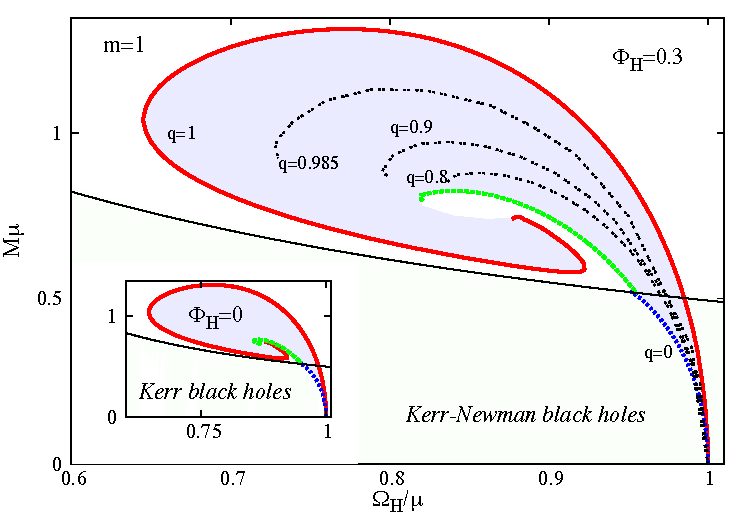
\includegraphics[width=0.497\textwidth]{papers/KerrNewman/BH-w-M}
     \includegraphics[width=0.497\textwidth]{papers/KerrNewman/zoom-w-M}
  \end{center}
  \caption{The $(\Omega_H,M)$ domain of existence for a sample of KNBHsUSH. (Main left panel) Diagram for $\Phi_H=0.3$ with the boson star envelope (red solid line), the existence line on the domain of KN BHs (blue dotted line) and the line of extremal KNBHsUSH (green dashed line). The black solid line corresponds to the extremal KN BHs; non-extremal solutions exist below. The black dotted lines have constant normalized Noether charge $q$. (Inset) diagram for $\Phi_H=0$, for comparison. (Right panel) Detail around the intersection of the existence lines with the extremal KNBHsUSH lines and the extremal KN lines for $\Phi_H=0,0.6$ and $0.8$.  
	}
  \label{fig:w-M}
\end{figure}
%%%%%%%%%%%%%%%%%%%%%%%%%%%%%%%%%%%%%%%%%%%%%%%%%%%%%%%%%%%
 
  
 In Fig.~\ref{fig:w-g} (left panel), we exhibit the ratio $ M^{\Psi}/M$, which gives another measure of hairiness
   as a function of $\Omega_H$,
for $\Phi_H=0.3$. The figure shows that small fractions of the total energy in the hair are only allowed for sufficiently large horizon angular velocity. When the angular velocity is small, equilibrium between the hair and the horizon is only possible for solutions with $q$ close to unity, $i.e.$, boson star-like. 
The inset in this figure shows the $(\Omega_H,Q_E)$ domain of existence of the KNBHsUSH solutions. It illustrates that the electric charge of the solutions, for fixed $\Omega_H$ between that of the Hod point and the maximum allowed frequency, $\Omega_H=\mu$, is maximized along the existence line (and in particular at the Hod point). But for lower values of the frequency, slightly larger charges than that found at the Hod point are possible, occurring along the extremal hairy BHs line.

 

 

%%%%%%%%%%%%%%%%%%%%%%%%%%%%%%%%%%%%%%
\subsubsection{Gyromagnetic ratio}
%%%%%%%%%%%%%%%%%%%%%%%%%%%%%%%%%%%%%%
Rotating charges give rise to a magnetic dipole moment, $\mu_M$. 
In classical electromagnetism, a generic relation of the form~\eqref{gyro}, 
between $\mu_M$ and the total angular momentum, mass and charge can be derived, 
for systems with constant ratio of charge to mass density, yielding $g=1$. 
When experiments such as that performed for Stern and Gerlach in the early XXth century, 
showed that the electron should have $g=2$, it became clear that a new fundamental description 
for the electron was necessary, beyond the scope of the non-relativistic quantum theory. 
Such a description appeared with the Dirac equation, which, from first principles predicts $g=2$, 
a value that is corrected by loop diagrams in Quantum Electrodynamics (QED), 
yielding the so called anomalous magnetic moment, whose agreement 
with experiment is one of the outstanding successes of QED.

In BH physics, Carter first observed that $g=2$ for the KN solution. 
Since then many other studies considered the gyromagnetic ratio of rotating charged BHs, 
for instance with different asymptotics and in higher dimensions (see $e.g.$~
\cite{Garfinkle:1990ib,Herdeiro:2000ap,Aliev:2004ec,Ortaggio:2006ng,Aliev:2006tt}). 
Here we show that the addition of scalar hair leads to a suppression of the gyromagnetic ratio, 
and of the corresponding magnetic dipole moment, 
with respect to that of a comparable KN BH.  
 A novel aspect is that $g$ 
can be smaller than 1, a rather unsual feature in other models of relativistic, 
charged and spinning compact objects, 
$cf.$~\cite{Novak:2003uj}. 


In Fig.~\ref{fig:w-g} (right panel), we exhibit the gyromagnetic ratio in a $(q,g)$-diagram, for KNBHsUSH with $\Phi_H=0.3$.
The diagram shows that the gyromagnetic ratio, $g$, of both the extremal and non-extremal hairy BH solutions, is always less than $2$.
As expected, it does approach $2$, for both cases, in the limit of vanishing hair.
Further insight is obtained by considering the quantity
\begin{eqnarray}
\Delta\equiv \frac{M^2}{Q_E^2+J^2/M^2} \ ,
\end{eqnarray}
which determines the KN bound $\Delta\geqslant 1$. Indeed, all KN BHs have $\Delta>1$. This bound is, however, violated by a large set of KNBHsUSH, in particular by those close to the BS limit. This is reminiscent of what has been found for KBHsSH - see the discussions in~\cite{Herdeiro:2014goa,Herdeiro:2015gia,Herdeiro:2015tia,Delgado:2016zxv}.  Our results show that
solutions with $g<1$ predominantly exhibit $\Delta<1$ and thus violate the KN bound -- $cf.$ the inset of Fig.~\ref{fig:w-g} (right panel).



%%%%%%%%%%%%%%%%%%%%%%%%%%%%%%%%%%%%%%%%%%%%
\begin{figure}[H]
  \begin{center}
    \includegraphics[width=0.497\textwidth]{papers/KerrNewman/Mpsi}
      \includegraphics[width=0.497\textwidth]{papers/KerrNewman/qg}
  \end{center}
  \caption{(Left panel) The ratio $M^\Psi/M$ is shown as a function of $\Omega_H$ for a sample of KNBHsUSH. The inset shows the electric charge as a function of $\Omega_H$, where the blue dotted line is the existence line. 
	(Right panel)  The $(q,g)$ space. The inset show $g$ as a function of $\Delta$, that determines the KN bound.
}
\label{fig:w-g} 
\end{figure}
%%%%%%%%%%%%%%%%%%%%%%%%%%%%%%%%%%%%%%%%%%%%

 
 


%%%%%%%%%%%%%%%%%%%%%%%%%%%%%%%%%%%%%%%%%%%%
\section{Gauged scalar field model}
\label{sec_mod_g}
%%%%%%%%%%%%%%%%%%%%%%%%%%%%%%%%%%%%%%%%%%%%




%%%%%%%%%%%%%%%%%%%%%%%%%%%%%%%%
\subsection{Main differences in the model}

%%%%%%%%%%%%%%%%%%%%%%%%%%%%%%%%

Let us now consider the model described in Section~\ref{sec_mod_u} but with a \textit{gauged} scalar field, 
that couples minimally to the electromagnetic field, with gauge coupling $q_E$. 
This coupling is implemented by replacing the partial derivatives of the scalar field in the action~\eqref{action} as
\begin{equation}
\partial_a \Psi \longrightarrow D_a\Psi=\partial_a \Psi + iq_E A_a \Psi \ .
\label{mc}
\end{equation}
The Einstein equations still take the form~\eqref{eom}, but with the substitution~\eqref{mc} 
in the scalar field energy-momentum tensor~\eqref{emt}. Then, the scalar and Maxwell equations of motion become
\begin{eqnarray}
\label{field-eqs}
D_{a}D^{a}\Psi=\mu^2 \Psi\ , \qquad 
\nabla_{b}F^{ba}=
iq_E \big [ (D^{a}\Psi^*) \Psi-\Psi^*(D^a \Psi) \big ] 
\equiv q_E j^a  \ .
\end{eqnarray}  
Physically, the scalar field is now electrically charged 
(its quanta, the scalar particles, carry a charge $q_E$), and thus the scalar field sources the Maxwell field.

This model is invariant under the $local$ U(1) gauge transformation 
\begin{eqnarray}
\label{gauge-transf}
\Psi \to \Psi e^{-i q_E \alpha}\ ,~~A_a\to A_a+\partial_a \alpha \ ,
\end{eqnarray}
where $\alpha$ is a real function. One consequence of this gauge invariance is that the $(t, \varphi)$-dependence of the scalar field ansatz~\eqref{scalar_ansatz}, 
can now be gauged away by applying the local $U(1)$ symmetry
(\ref{gauge-transf})
with $\alpha =  (m\varphi -w t)/q_E$.  This, however, also changes the gauge field, as $A_t\to A_t-w/q_E$,
$A_\varphi \to A_\varphi+m/q_E$. 
%
Consequently, the solutions cannot be constructed starting with the configurations in the
previous sections and increasing $q_E$.
%
Thus, in order
to be able to consider this approach, we  keep the $(t,\varphi)$-dependence in 
the scalar field ansatz and fix the corresponding gauge freedom by setting $A_t = A_\varphi = 0$ at infinity.

One major difference with respect to the case 
discussed in the previous section 
 is that the solitonic limit of the solutions carries now a nonzero electric charge.
Self-gravitating charged boson stars were first considered, in spherical symmetry, in~\cite{Jetzer:1989av} 
(see also the recent work  \cite{Pugliese:2013gsa}). 
To the best of our knowledge, no rotating generalizations of these static solutions have been reported\footnote{ 
Some properties of the spinning charged solitons, 
with a self-interacting ($Q$-ball type) scalar field model, were addressed in~\cite{Brihaye:2009dx}.
}.
The Noether charge $Q$ of the solitons, $i.e.$ the total
particle number, is now intrinsically related to the electric charge $Q_E$. 
The former can be computed as  
%
\begin{eqnarray}
\label{Q1}
Q= \int j^t \sqrt{-g} dr  d\theta d\varphi=
 4\pi \int_{0}^\infty dr \int_0^\pi d\theta  
~r^2\sin \theta ~e^{-F_0+2F_1+F_2}  (w-q_E A_t -mW)\phi^2 \ ,
\end{eqnarray}
%
whereas the latter is read from the asymptotics
 of the electric potential $A_t$, as given in  (\ref{asym-matter-fields}). 
A straightforward computation 
shows that both the Noether charge and the electric charge of the spinning \textit{solitons}
are proportional  to the total angular momentum,
\begin{eqnarray}
\label{JQ}
J= m Q=\frac{4 \pi m Q_E}{q_E}\ .
\end{eqnarray} 


%%%%%%%%%%%%%%%%%%%%%%%%%%%%%%%%%%%%%%%%%%%%%%%%%%%%%%%%%%%%%%%%%%
\subsection{Features of the gauged scalar field solutions}
\label{sec_results_g}
%%%%%%%%%%%%%%%%%%%%%%%%%%%%%%%%%%%%%%%%%%%%%%%%%%%%%%%%%%%%%%%%%%
 
The construction of the  gauged scalar field solutions is similar 
to that described above for the ungauged case ($q_E=0$ limit).
In particular, the KNBHsGSH are subject to the same set of 
boundary conditions  used in the ungauged case.
The synchronization condition, however, is different,   
\begin{equation}
\label{cond-new}
 w-q_E \Phi_H=m \Omega_H \ ,
\end{equation}
in agreement with the result found in the linear theory~\cite{Hod:2014baa,Benone:2014ssa}.



The electrically charged boson stars also form a part of the domain of existence of KNBHsGSH. 
Thus we have paid special attention to this limiting case.
These solutions  are obtained by considering the ansatz~\eqref{metric_ansatz}--\eqref{electric_ansatz} with $r_H=0$ 
and replacing the boundary conditions at the horizon~\eqref{bch1} 
by the following boundary conditions at the origin
\begin{eqnarray}
\label{bc0} 
\partial_r F_i|_{r=0}= 
W|_{r=0}=0\ ,~~
\phi| _{r =0}=0\ ,~~\partial_r A_t|_{r=0}=A_\varphi|_{r=0}=0\ .
\end{eqnarray}
% 

Some results of the numerical integration are shown in Fig.~\ref{fig:w-M-gauged} (left panel).
The basic properties of the spinning gauged boson stars solutions can be summarized as follows.
First, for all values of the gauge coupling considered so far, 
the frequency dependence of the solutions is qualitatively similar to the ungauged case.
The solutions 
exist for a limited range of frequencies
$0<w_{min}<w<\mu$. 
In particular, we observe that the minimal frequency increases with $q_E$. 
After this minimal frequency, a backbending towards larger values of $w$ occurs, yielding a second branch of solutions. 
A second backbending, towards
smaller values of $w$,  is observed as the frequency reaches a maximal value along the second branch, $w\to w_{max}$, whose value increases again with $q_E$. 
Then, similarly to the ungauged limit, a third branch of solutions develops -- not shown in Fig.~\ref{fig:w-M-gauged} (left panel).
Subsequently, we expect the existence of an inspiraling behaviour of the solutions, 
in analogy with uncharged boson stars, towards a limiting configuration.  


%%%%%%%%%%%%%%%%%%%%%%%%%%%%%%%%%%%%%%%%%%%%%%%%%%%%%%%%%%%
\begin{figure}[H]
  \begin{center}
    \includegraphics[width=0.497\textwidth]{papers/KerrNewman/BS-w-M-gauged}
      \includegraphics[width=0.497\textwidth]{papers/KerrNewman/BS-g-M-gauged}
  \end{center}
  \caption{
	(Left panel)
	The $(w,M)$ diagram for spinning boson stars with $q_E=0$ (red curve), $q_E/\mu=0.2, 0.3, 0.4, 0.5$
	and $0.6$ (top curve).  
		(Right panel)
	The mass $M$ is shown as a function of the gauge coupling constant $q_E$
	for several frequencies, $w/\mu=0.7, 0.8, 0.9$ and $0.95$ (as an inset).	}
  \label{fig:w-M-gauged}
\end{figure}
 %%%%%%%%%%%%%%%%%%%%%%%%%%%%%%%%%%%%%%%%%%%%%%%%%%%%%%%%%%%
Although only the mass is displayed in Fig.~\ref{fig:w-M-gauged} (left panel), the $J(w)$
diagram has a very similar shape.
Consequently,  the axially symmetric gauged boson stars do not possess
a static limit.  Observe also that the maximal mass of spinning gauged boson stars solutions increases with $q_E$.


As shown in Fig.~\ref{fig:w-M-gauged} (right panel), 
the solutions possess also a nontrivial dependence on 
the gauge coupling constant $q_E$.
For given values of $w$,
spinning solutions exist up to a maximal
value of the gauge coupling constant only, $q_E=(q_E)_{max}$.
The physics rationale behind this behaviour 
is similar to that discussed for the spherically symmetric case 
\cite{Jetzer:1989av,Pugliese:2013gsa}.
For $q_E>(q_E)_{max}$ the charge repulsion  becomes bigger than
  the scalar and gravitational attraction and localized solutions cease to exist  
(note that the maximal value of $q_E$
increases with frequency).
Also, as seen in Fig.~\ref{fig:w-M-gauged} (right panel),
all global charges stay finite as $q_E\to (q_E)_{max}$.
 

KNBHsGSH are obtained by adding a horizon at the center of the spinning gauged boson star  
we have just described, which can be done for  any such  solution.
One way to construct the BHs
  is to  start from  boson stars 
and slightly increase the horizon size via the parameter $r_H$.
In this approach, the other input parameters 
$\Omega_H$, $q_E$,  $\Phi_H$ and $m$
are kept fixed. 
We recall that for BHs, the frequency $w$ is fixed by the synchronization condition (\ref{cond-new}).
Then one finds three 
possible behaviours for
the resulting branches of BH solutions -- see Fig.~\ref{fig:q-AH-gauged} (left panel).
 First  ($i$), for small enough values of $\Omega_H$,
 the branch of BHs connects two different boson stars; 
as $r_H\to 0$ the horizon area vanishes, $q\to 1$, while the temperature
 diverges.
For intermediate values of  $\Omega_H$,
the branch of solutions ends in an extremal KNBHsGSH solution ($ii$). 
These limiting configurations have finite
horizon size   and global charges, $0<q<1$ and appear to possess 
a regular horizon.
Finally   ($iii$), for large values of $\Omega_H$,
the branch of  KNBHsGSH interpolates between 
a charged boson star and a set of critical KN solutions (with $q=0$ and $A_H>0$), which lies again 
on an {\it existence line}. 

 In Fig.~\ref{fig:q-AH-gauged} (right panel) we exhibit the (Komar) energy density and angular momentum density (in the inset) for an illustrative example of a KNBHGSH  with physical input parameters 
$r_H=0.24, w =0.86, q_E =0.2, \Phi_H=0.1$. 
These densities have a contribution from both the electromagnetic and the scalar field. The main feature we wish to emphasize is the composite structure revealed by the plots. KN BHs have an (electromagnetic) energy and angular momentum density that decays with the radial coordinate, whereas KBHsSH 
(and boson stars)
have toroidal-like distributions for the (scalar) energy and angular momentum densities. 
Consequently, KNBHsGSH exhibit a superposition of these two behaviours, with decaying densities from the horizon but which exhibit a local maximum, in the neighbourhood of the equatorial plane, at some finite radial coordinate. 
A similar energy and angular momentum distribution can be found for KNBHsUSH.  

The behaviours illustrated in Fig.~\ref{fig:q-AH-gauged} supports the expectation that the domain of existence of KNBHsGSH will fill in the domain delimited by the boson star curves exhibited in Fig.~\ref{fig:w-M-gauged} (left panel), together with the existence line of KN BHs and a line of extremal KNBHsGSH,  in a qualitatively similar fashion to that shown in Fig.~\ref{fig:w-M} (left panel). Having established these solutions exist, and that their domain of existence will be analogue to the case of KNBHsUSH, we will not enter further details here; its systematic and detailed study will be reported elsewhere.
Here we mention only that, similar to the ungauged case, 
the gyromagnetic ratio of  KNBHsGSH constructed so far is always smaller than $g=2$.


%%%%%%%%%%%%%%%%%%%%%%%%%%%%%%%%%%%%%%%%%%%%%%%%%%%%%%%%%%%
\begin{figure}[H]
  \begin{center}
    \includegraphics[width=0.497\textwidth]{papers/KerrNewman/BH-q-AH} 
      \includegraphics[width=0.497\textwidth]{papers/KerrNewman/energy-2d} 
  \end{center}
  \caption{ (Left panel) 
	The $(A_H,q)$ diagram is shown for three sets of KNBHsGSH solutions with fixed values of 
$\Omega_H$ and 
$q_E/\mu=0.2$, 
$\Phi_H=0.1$. (Right panel) 
 Energy density (and angular momentum density in the inset) along three different slices of constant $\theta$ for an illustrative example of a KNBHGSH.
	}
  \label{fig:q-AH-gauged}
\end{figure}
 %%%%%%%%%%%%%%%%%%%%%%%%%%%%%%%%%%%%%%%%%%%%%%%%%%%%%%%%%%%
 


%%%%%%%%%%%%%%%%%%%%%%
\section{Remarks}
\label{sec_remarks}
%%%%%%%%%%%%%%%%%%%%%%%

The Kerr solution~\cite{Kerr:1963ud}, which describes the paradigmatic BH geometry in General Relativity, allows a generalization with electric (or magnetic) charge~\cite{Newman:1965my}, discovered shortly after the Kerr metric. Much more recently, it was found that the Kerr solution also allows a generalizations with scalar~\cite{Herdeiro:2014goa,Herdeiro:2015gia,Kleihaus:2015iea,Herdeiro:2015tia,Chodosh:2015oma} or Proca hair~\cite{Herdeiro:2016tmi}. The former are known as Kerr BHs with scalar hair (KBHsSH). In this paper we have added electric charge to KBHsSH, both considering an ungauged and a gauged scalar field and analysed some basic properties of the solutions. In both cases, their domain of existence is qualitatively similar to the of the uncharged hairy BHs. In particular it is bounded by three curves, corresponding do the solitonic limit (boson stars), extremal hairy BHs, and bald (KN) BHs. In the gauged case, the solitonic limit corresponds to rotating charged boson stars, which hitherto have not been studied in the literature. 

As an example of a novel physical property of these solutions we have considered the gyromagnetic ratio, $g$. This quantity measures how a magnetic dipole moment is induced by the charge and angular momentum of the BH. It is well known the relativistic (Dirac) value holds for the KN BH, $g=2$~\cite{Carter:1968rr}. We have shown that the gyromagnetic ratio of these hairy charged BHs is always $g\leqslant 2$, with equality attained only in the ``bald" case. Thus, the scalar hair leads to a suppression of the magnetic dipole moment. Preliminary work (not reported herein), analysing the electromagnetic field lines of the BHs, suggests that the scalar hair also suppresses the higher electric multipole moments. We hope to give a detailed account of this behaviour in the near future.




There are other interesting applications for these solutions. As an example we mention testing the no-short hair conjecture. As originally stated~\cite{Nunez:1996xv}, this conjecture suggested that, when hair exists around a spherically symmetric BH, the `hair' should extend
beyond $3r_+/2$, where $r_+$ is the areal radius of the event horizon. This radius coincides with the location of the
circular null geodesic for the Schwarzschild solution, which led to an improved version of the conjecture that the hair must extend beyond the null circular orbit of the spacetime~\cite{Hod:2011aa}. For rotating BHs, an analysis of linearized hair suggested the no-short hair conjecture holds for uncharged BHs~\cite{Hod:2016dkn}, but may be violated for electrically charged ones~\cite{Hod:2014sha,Hod:2015ynd}. The latter possibility can be tested using the fully non-linear solutions of the Einstein-Maxwell-Klein-Gordon field equations reported in this paper. 








%%%%%%%%%%%%%%%%%%%%%%%%%%%%%%%%%%%%%%%%%%%%%%%%%%%%%%%%%%%%%%%%%%%%%%%%%%%%%%
\section*{Acknowledgements}
%%%%%%%%%%%%%%%%%%%%%%%%%%%%%%%%%%%%%%%%%%%%%%%%%%%%%%%%%%%%%%%%%%%%%%%%%%%%%%
C. H. and E. R. acknowledge funding from the FCT-IF programme. H.R. is supported by the grant PD/BD/109532/2015 under the MAP-Fis Ph.D. programme. This  work  was  partially  supported  by  the  H2020-MSCA-RISE-2015  Grant  No. StronGrHEP-690904,  and  by  the  CIDMA  project  UID/MAT/04106/2013.  Computations were performed at the BLAFIS cluster, in Aveiro University.
 \documentclass{article}
\usepackage{amsmath}
\usepackage{amssymb}
\usepackage{mathrsfs}
\usepackage{graphicx}
\usepackage{float}
\usepackage{caption}
\usepackage{subcaption}


\usepackage{epsfig}
\usepackage{amsmath}
\usepackage{amsfonts}
\usepackage{graphicx}


\usepackage[margin=2cm]{geometry}

\newcommand\scalemath[2]{\scalebox{#1}{\mbox{\ensuremath{\displaystyle #2}}}}

\begin{document}





\title{{\bf \Large Electrically charged \\ Kerr black holes with scalar hair}}

\vspace{0.5cm}

 \author{
 {\large Jorge F. M. Delgado}\footnote{jorgedelgado@ua.pt}, \
{\large Carlos A. R. Herdeiro}\footnote{herdeiro@ua.pt}, \
{\large Eugen Radu}\footnote{eugen.radu@ua.pt}  \ and
{\large Helgi R\'unarsson}\footnote{helgi.runarsson@ua.pt}
\\ 
\\
{\small Departamento de F\'\i sica da Universidade de Aveiro and} \\ 
{\small Center for Research and Development in Mathematics and Applications (CIDMA)} \\ 
{\small   Campus de Santiago, 3810-183 Aveiro, Portugal}
}


 
 
%%%%%%%%%%%%%%%%
%%%   DATE   %%%
%%%%%%%%%%%%%%%%

\date{August 2016}
\maketitle

%%%%%%%%%%%%%%%%%%%%
%%%   ABSTRACT   %%%
%%%%%%%%%%%%%%%%%%%%
\begin{abstract}
We construct electrically charged Kerr black holes (BHs) with scalar hair. 
Firstly, we take an uncharged scalar field, 
interacting with the electromagnetic field only indirectly,  via the background metric. 
The corresponding family of solutions, 
dubbed Kerr-Newman BHs with ungauged scalar hair, 
reduces to (a sub-family of) Kerr-Newman BHs in the limit of vanishing scalar hair 
and to uncharged rotating boson stars in the limit of vanishing horizon. 
It adds one extra parameter to the uncharged solutions: the total electric charge. 
This leading electromagnetic multipole moment is unaffected by the scalar hair 
and can be computed by using Gauss's law on any closed 2-surface surrounding  
(a spatial section of) the event horizon. 
By contrast, the first sub-leading electromagnetic multipole -- the magnetic dipole moment --, 
gets suppressed by the scalar hair, such that the gyromagnetic ratio is always smaller than the Kerr-Newman value ($g=2$).  
Secondly, we consider a gauged scalar field and obtain a family of Kerr-Newman BHs with gauged scalar hair. 
The  electrically charged scalar field now stores a part of the total electric charge, 
which can only be computed by applying Gauss' law at spatial infinity 
and introduces a new solitonic limit -- electrically charged rotating boson stars. 
In both cases, we analyse some physical properties of the solutions.
\end{abstract}


%\tableofcontents

%\newpage


%%%%%%%%%%%%%%
\section{Introduction}
%%%%%%%%%%%%%%
The Kerr metric~\cite{Kerr:1963ud} is the fundamental BH solution in General Relativity, believed to describe an untold number of BHs in (or near) equilibrium in the Cosmos. It is straightforward to generalize this solution to include an electric (or magnetic) charge, yielding the Kerr-Newman (KN) solution~\cite{Newman:1965my}. The latter is, perhaps, of a more limited astrophysical interest, as electric charge is expected to be residual in astrophysical BHs, due to efficient discharge mechanisms (but see the discussion in~\cite{Cardoso:2016olt}). Theoretically, however, the KN solution introduces some qualitatively new features, with respect to its vacuum counterpart, including: a (Komar) energy and angular momentum component outside the horizon~\cite{Delgado:2016zxv}; a more general extremal limit with different (including supersymmetric, when embedded in supergravity~\cite{Gibbons:1982fy,Tod:1983pm,Herdeiro:2000ap}) properties, depending on the electric charge; and a dipole magnetic moment, induced by the electric charge and the rotation. The corresponding gyromagnetic ratio turns out to have precisely the (non-anomalous) electron value, $g=2$~\cite{Carter:1968rr}. Moreover, the KN solution provides an arena for the study of the fully non-linear interplay between electromagnetism and gravity, in the framework of Einstein's theory, with often challenging properties, as for instance its stability -- see, $e.g.$, the discussions in~\cite{Pani:2013ija,Pani:2013wsa,Zilhao:2014wqa}.

\bigskip

As recently discovered, the Kerr solution admits also families of generalizations with scalar hair~\cite{Herdeiro:2014goa,Herdeiro:2015gia,Kleihaus:2015iea,Herdeiro:2015tia,Chodosh:2015oma} (and also Proca hair~\cite{Herdeiro:2016tmi}). In its simplest guise~\cite{Herdeiro:2014goa,Herdeiro:2015gia}, a non-trivial distribution of a complex, massive scalar field can be added to Kerr BHs, keeping them asymptotically flat and regular on and outside the event horizon. Such a scalar field carries a conserved Noether charge, but which, unlike the electric charge, is not associated to a Gauss law. As such, it cannot be computed as a flux integral at infinity; it must be evaluated by a volume integral, summing up the appropriate component(s) of the conserved Noether current, from infinity up to the horizon. These solutions have an intimate connection to the superradiant instability of Kerr BHs~\cite{Herdeiro:2014ima}, in the presence of a massive scalar field (see~\cite{Brito:2015oca} for a review). They bifurcate from Kerr for particular backgrounds that can support a stationary scalar cloud in the linear theory~\cite{Hod:2012px,Hod:2013zza,Herdeiro:2014goa,Benone:2014ssa,Hod:2015ota,Hod:2015goa}, and reduce to boson stars~\cite{Schunck:2003kk}, horizonless gravitating solitons, when the horizon area vanishes. Kerr BHs with scalar hair (KBHsSH) can have phenomenological properties distinct from Kerr, for instance their shadows~\cite{Cunha:2015yba}. This fact, in view of the various observations/experiments that promise to deliver detailed information on BH candidates and strong gravity in the near future, makes their analysis in the astrophysical context quite timely -- see~\cite{Vincent:2016sjq,Ni:2016rhz} for recent examples of such phenomenological studies.

\bigskip

It is expectable that KBHsSH, just like the Kerr solution, admit electrically charged generalizations. Again, the astrophysical interest of such solutions is, perhaps, more limited, but understanding their existence and their physical properties is of relevance to fully grasp the impact of this scalar (or other) hair on the paradigmatic BHs of General Relativity. The purpose of this paper is, precisely, to construct examples of such electrically charged generalizations of KBHsSH and to examine some of their physical properties. 

\bigskip

We shall focus on Einstein--Maxwell--(complex)Klein-Gordon theory, where the scalar field is massive and has no self-interactions. All couplings, moreover, are minimal. We start by considering an ungauged (hence electrically uncharged) scalar field. In this case, the family of solutions -- Kerr-Newman BHs with ungauged scalar hair (KNBHsUSH) -- is described by four continuous parameters (with one non-trivial constraint between them): $(1)$ the ADM mass, $M$, which can be split into the horizon and exterior matter/energy contribution (composed of the scalar $\Psi$ plus electromagnetic fields), $M=M_{\rm H}+M^\Psi+M^{\rm EM}$; $(2)$ the total angular momentum, $J$, which can also be split in a similar fashion, $J=J_{\rm H}+J^\Psi+J^{\rm EM}$; $(3)$ the  Noether charge, $Q$, associated to the global $U(1)$ invariance of the complex scalar field, which obeys $Q=mJ^\Psi$, where $m$ is the azimuthal winding number; $(4)$ and the total electric charge, $Q_E$. All electric charge is contained within the BH horizon, $Q_E=Q_E^{\rm H}$, whereas all Noether charge is contained outside the horizon. By Gauss's law the former can be computed by the flux of the electric field on any closed 2-surface surrounding the horizon, and is unaffected by $Q$. The magnetic dipole moment, on the other hand, which is induced by the electric charge in the rotating spacetime, is affected by the Noether charge, with respect  to the KN value. This is appropriately described by the gyromagnetic ratio, which is $g=2$ for KN and it is $g\leqslant 2$ for the hairy BHs. Thus, for the same amount of total mass, angular momentum and electric charge, KNBHsUSH have less magnetic dipole moment, a suppression of the magnetic dipole due to the scalar hair. The domain of existence of KNBHsUSH is bounded by (a particular set of) KN BHs, when $Q=0$; a set of extremal (zero temperature) BHs; and (electrically uncharged) rotating boson stars, when $Q_E=0$, for which $M=M^\Psi$ and $J=J^\Psi=mQ$.  As for the uncharged KBHsSH, there is no static limit for KNBHsUSH.

\bigskip

Gauging the scalar field, with a gauge coupling $q_E$, hence endowing the scalar particles with electric charge, leads to a family of KN BHs with gauged scalar hair (KNBHsGSH), which exhibits some changes with respect to the previously discussed KNBHsUSH. 
%
Firstly, as in the ungauged case,
both the mass and the angular momentum can be split  into the horizon and exterior contribution.
However, the corresponding parts for the electromagnetic and  the scalar $\Psi$ fields cannot be rigorously
separated since  here they interact directly, not only via the spacetime geometry.
Moreover this time  
the total electric charge has both a horizon and a contribution sourced by the scalar field,  $Q=Q^{\rm H}_E+Q^\Psi_E$,  
and needs to be calculated by the asymptotic flux.
$Q_E^\Psi$ is determined by the total Noether charge, which counts the number of the scalar particles, multiplied by their individual electric charge:  $Q_E^\Psi=q_E Q/(4 \pi)$. 
This redistribution of the electric charge, does not, however change the qualitative behaviour of the gyromagnetic ratio. 
For all solutions constructed so far we still observe that it is always $g\leqslant 2$, with equality attained for the KN case. 
The boundaries of the domain of existence of KNBHsGSH are sensitive to the gauging. 
Both the KN, extremal and solitonic limits are different. 
In particular, the latter is a set of rotating  boson stars with  $nonzero$ electric 
and magnetic fields, for which  $Q_E= q_E Q/(4\pi)= q_E J/(4 \pi m)$.  

 
\bigskip

This paper is organized as follows. In Section~\ref{sec_mod_u} we describe the ungauged scalar field model, the boundary conditions, physical quantities of interest and the numerical results for the domain of existence of the solutions, as well as some physical properties, including the gyromagnetic ratio. A similar, albeit less extensive analysis, is performed in Section~\ref{sec_mod_g} for the gauged case, emphasizing the differences with respect to the ungauged one. Finally, in Section~\ref{sec_remarks} we present some closing remarks.



%%%%%%%%%%%%%%%%%%%%%%%%%%%%%%%%
\section{The ungauged scalar field model}
\label{sec_mod_u}
%%%%%%%%%%%%%%%%%%%%%%%%%%%%%%%%


%%%%%%%%%%%%%%%%%%%%%%%%%%%%%%%%
\subsection{Action, equations of motion and ansatz}
\label{sec_mofrl}
%%%%%%%%%%%%%%%%%%%%%%%%%%%%%%%%
We start by considering Einstein--Maxwell theory, minimally coupled to a complex, massive (mass $\mu$)  ungauged scalar field $\Psi$.  The corresponding action is
%
%
\begin{eqnarray}
  \label{action}
 \mathcal{S} = \frac{1}{4\pi G}\int d^4x \sqrt{-g}\left[\frac{R}{4}- \frac{1}{4}F_{ab}F^{ab}- g^{ab}\Psi^*_{,a}\Psi_{,b} -\mu^2\Psi^*\Psi \right]\ ,  
\end{eqnarray}  
where $F_{ab}$ are the components of the Maxwell 2-form, $F$, related to the 1-form potential $A=A_adx^a$ as $F=dA$. The Einstein--Klein-Gordon--Maxwell equations, obtained by varying the action with respect to the metric, scalar field and electromagnetic field, are, respectively,
%
%
\begin{equation}
G_{ab}  = 2\left( T_{ab}^\Psi+T_{ab} ^{\rm EM} \right)\ , \qquad \Box \Psi =\mu^2\Psi \ , \qquad D_aF^a_{~b}=0 \ ,
\label{eom}
\end{equation}
where the two components of the energy-momentum tensor are
%
\begin{equation}
\label{emt}
T_{ab}^\Psi \equiv  
 \Psi_{ , a}^*\Psi_{,b}
+\Psi_{,b}^*\Psi_{,a} 
-g_{ab}  \left[ \frac{1}{2} g^{cd} 
 ( \Psi_{,c}^*\Psi_{,d}+
\Psi_{,d}^*\Psi_{,c} )+\mu^2 \Psi^*\Psi\right] \ , \qquad
 T_{ab}^{\rm EM} \equiv F_a^{~c}F_{bc} - \frac{1}{4}g_{ab}F_{cd}F^{cd} \ .
\end{equation}
This model is invariant under a \textit{global} transformation $\Psi\rightarrow \Psi e^{i\alpha}$, where $\alpha$ is constant.



KNBHsUSH are obtained using the metric, scalar field and electromagnetic potential ansatz given by
%
\begin{align}
  \label{metric_ansatz}
  ds^2 &= -e^{2F_0}Ndt^2 + e^{2F_1}\left( \frac{dr^2}{N} + r^2d\theta^2 \right) + e^{2F_2}r^2\sin^2\theta \left(d\varphi - Wdt \right)^2 \ ,\\
\label{scalar_ansatz}
\Psi &= \phi(r,\theta)e^{i(m\varphi-w t)}~, \\
 \label{electric_ansatz}
 A_adx^a &= \left( A_t - A_\varphi W\sin\theta \right)dt + A_\varphi\sin\theta d\varphi \ ,
\end{align}
where $N\equiv 1-r_H/r$ and $r_H$ is a constant describing the event horizon location in this coordinate system; the metric ansatz functions $F_i,W$, $i=0,1,2$, as well as $\phi$, $A_t$ and $A_\varphi$, depend on the spheroidal coordinates $r$ and $\theta$ only; $w\in \mathbb{R}^+$ is the scalar field frequency and $m=\pm 1,\pm 2$\dots is the azimuthal harmonic index. In the following we shall focus on the case $m=1$ as an illustrative set of solutions, and also nodeless solutions for the scalar field profile $\phi$. Solutions with nodes will also exist, corresponding to excited states with higher ADM mass. 




%%%%%%%%%%%%%%%%%%%%%%%%%%%%%%%%
\subsection{Boundary conditions}
\label{sec_bc}
%%%%%%%%%%%%%%%%%%%%%%%%%%%%%%%%
In order to find KNBHsUSH, we use the numerical strategy and code already discussed in some of our previous works (see, $e.g.$~\cite{Herdeiro:2015gia,Herdeiro:2016tmi}). To obtain these solutions, appropriate boundary conditions must be imposed, that we now summarize.
  
At spatial infinity, $r\rightarrow\infty$, we require that the solutions approach a Minkowski spacetime
with vanishing matter fields:
\begin{equation}
  \lim_{r\rightarrow \infty}{F_i}=\lim_{r\rightarrow \infty}{W}=\lim_{r\rightarrow \infty}{\phi}=\lim_{r\rightarrow\infty}A_\varphi=\lim_{r\rightarrow\infty}A_t=0\ .
\end{equation}
(Observe that the last equality could be changed to a constant, rather than zero, in a different gauge.) 
%
%\item[$\bullet$] 
On the symmetry axis, $i.e.$ at $\theta=0,\pi$, axial symmetry and regularity require that
\begin{equation}
\partial_\theta F_i = \partial_\theta W = \partial_\theta A_t = \phi = A_\varphi = 0\ .
\end{equation} 
%
Moreover, all solutions herein are invariant under a reflection in the equatorial plane ($\theta=\pi/2$).
The event horizon is located at a surface with constant radial variable, $r=r_H>0$.
By introducing a new radial coordinate $x=\sqrt{r^2-r_H^2}$ 
the boundary conditions and numerical treatment of the problem are simplified.
Then one can write an approximate form of the solution  near the horizon as a power series in $x$,
which implies the following boundary conditions
\begin{equation}
\partial_x F_i \big|_{x=0}= \partial_x \phi  \big|_{x=0} =  0,~~W \big|_{x=0}=\Omega_H,~~
%\frac{w}{m},~~
A_t \big|_{x=0} =  \Phi_H,~~ \partial_x A_\varphi \big|_{x=0}=0 ,
\label{bch1}
\end{equation}
where $\Omega_H $ is the horizon angular velocity
and $\Phi_H$ is the horizon electrostatic potential. 
Similarly to the uncharged case, the existence of a smooth solution imposes also the
\textit{synchronization condition}
%
\begin{eqnarray}
\label{cond}
w=m\Omega_H\ .
\end{eqnarray}
%
 


%%%%%%%%%%%%%%%%%%%%%%%%%%%%%%%%
\subsection{Physical quantities}
\label{sec_pq}
%%%%%%%%%%%%%%%%%%%%%%%%%%%%%%%%
Axi-symmetry and stationarity of the spacetime (\ref{metric_ansatz})
 guarantee the existence of two conserved global charges, the total mass $M$ and angular momentum $J$, 
which can be computed either as Komar integrals at spatial infinity or, equivalently, 
from the decay of the appropriate metric functions:
%
\begin{eqnarray}
\label{asym}
g_{tt} =-e^{2F_0}N+e^{2F_2}W^2r^2 \sin^2 \theta 
\to
 -1+\frac{2GM}{r}+\dots, ~~
g_{\varphi t}=-e^{2F_2}W r^2 \sin^2 \theta
\to 
\frac{2GJ}{r}\sin^2\theta+\nonumber \dots.  
\end{eqnarray}
%
These quantities can be split into the horizon contribution -- computed as a Komar integral on the horizon -- and the matter contributions, composed of the scalar field and electromagnetic parts, computed as the volume integrals of the appropriate energy-momentum tensor components: 
%
\begin{eqnarray}
\label{MH-hor}
M=M^\Psi+M^{\rm EM}+M_H\ , \qquad J=J^\Psi+J^{\rm EM}+J_H\ ,
%J=mQ+J^{\rm EM}+J_H\ ,
\end{eqnarray}
where $M_H$ and $J_H$  are the horizon mass and angular momentum.
$M^\Psi$ and $J^\Psi$ are the scalar field energy and angular momentum outside the horizon,
with  
\begin{align}
\label{Mpsi}
-M^\Psi\equiv  \int_{\Sigma} dS^a (2T_{ab}^\Psi \xi^b-T^\Psi\xi_a)
 = 4\pi \int_{r_H}^\infty dr \int_0^\pi d\theta~r^2\sin \theta ~e^{F_0+2F_1+F_2}
 \left(
 \mu^2-2 e^{-2F_0}\frac{w(w-mW)}{N}
 \right)\phi^2 ~~,
\end{align}
while $J^\Psi=mQ$,
where $Q$ is the Noether charge 
associated with the the $global$ $U(1)$ symmetry of the complex scalar field 
\begin{eqnarray}
\label{Q-int}
Q=4\pi \int_{r_H}^\infty dr \int_0^\pi d\theta 
~r^2\sin \theta ~e^{-F_0+2F_1+F_2}  \frac{(w-mW)}{N}\phi^2 ~.
\end{eqnarray}
To measure the hairiness of a BH, it is convenient 
to introduce the normalized Noether charge
\begin{eqnarray}
\label{q}
q=\frac{mQ}{J}~,
\end{eqnarray}
with $q=1$ for solitons and $q=0$ for KN BHs.
%
Also, $M^{\rm EM}$ and $J^{\rm EM}$ are the mass and angular momentum stored in the electromagnetic field
outside the horizon.  
The solutions possess also an electric charge $Q_E$ that can be computed using Gauss's law, 
on any closed 2-surface covering the horizon. 
Alternatively, $Q_E$ can be computed from the decay of the 4-potential, together with the magnetic dipole moment $\mu_M$:
%
 \begin{eqnarray}
 \label{asym-matter-fields}
A_t\sim 
\frac{Q_E}{r}+\dots \ , \qquad A_{\varphi}\sim \frac{\mu_M \sin \theta}{r}+\dots\
 .
 \end{eqnarray}
As with the KN BHs, the gyromagnetic ratio $g$ defines how the magnetic dipole moment 
is induced by the total angular momentum and charge, for a given total mass:
 \begin{equation}
 \mu_M=g\frac{Q_E}{2M}J \ .
 \label{gyro}
 \end{equation}
 %
The BH horizon introduces a temperature $T_H$ and an entropy $S={A_H}/({4G})$,
where 
%
\begin{eqnarray}
\label{THAH}
T_H=\frac{1}{4\pi r_H}e^{(F_0-F_1)|_{r_H}}\ ,
\qquad
A_H=2\pi r_H^2 \int_0^\pi d\theta \sin \theta~e^{(F_1+F_2)|_{r_H}} \ .
\end{eqnarray}
%
The various quantities above are related by a Smarr mass formula 
%
\begin{eqnarray}
\label{smarr}
M=2 T_H S +2\Omega_H (J-m Q) + \Phi_H Q_E+ M^\Psi,
\end{eqnarray}
The solutions satisfy also the 1st law 
%
\begin{eqnarray}
\label{first-law}
dM=T_H dS +\Omega_H dJ + \Phi_H dQ_E\ .
\end{eqnarray}
%
Finally, observe that from \eqref{smarr} and \eqref{MH-hor} are consistent with a different Smarr relation, only in terms of horizon quantities  
%
%
\begin{eqnarray} 
\label{rel-hor}
M_H=2T_H S+2 \Omega_H J_H~,
% + \Phi_H Q_E \ .
\end{eqnarray}
together with the electromagnetic relation $M^{\rm EM}=\Phi_HQ_E+2\Omega_HJ^{\rm EM}$.




%%%%%%%%%%%%%%%%%%%%%%%%%%%%%%%%%%%%%%%%%%%%
\subsection{The results }
\label{sec_results_u}
%%%%%%%%%%%%%%%%%%%%%%%%%%%%%%%%%%%%%%%%%%%%
As in the previous work \cite{Herdeiro:2015gia,Herdeiro:2016tmi}
the numerical integration is performed with 
dimensionless variables introduced by using natural units set by $\mu$ and $G$.
The global charges and all other quantities of interest are also
 expressed in units set by $\mu$ and $G$ 
(we set $G=1$ in what follows). 
In particular this means we set $\mu Q_E\rightarrow Q_E$; 
note that $\Phi_H$ is dimensionless (in units such that $4\pi \epsilon_0=1$). 

Let us start by getting an overview of the domain of existence of KNBHsUSH. 
This requires fixing the new degree of freedom, related to electric charge. 
An important observation here is that, similarly to the
KN case, no solitonic limit exists, for a nonzero $Q_E$.
Thus, for most of the numerical solutions we have chosen to fix the electrostatic potential on the horizon $\Phi_H$
and vary the remaining  input parameters $\Omega_H$ and $r_H$.
This allows these  two-dimensional sections of the full domain of existence to reach the solitonic limit, 
wherein the horizon area vanishes and the electrostatic potential becomes constant everywhere and pure gauge.


 In Fig.~\ref{fig:w-M} (left panel), 
we exhibit the $(\Omega_H,M)$ domain of existence of the solutions, where we have fixed the horizon electrostatic potential to be $\Phi_H=0.3$. Observe that the domain therein was obtained by extrapolating into the continuum
the results from discrete sets of around two thousand numerical solutions; we also remark that a qualitatively similar picture has been found for $\Phi_H=0.6$.
 As shown in the main panel (the inset is for $\Phi_H=0$), 
this domain of existence is bounded by boson stars (red solid line), 
the KN limit (blue dotted line -- dubbed \textit{existence line}) 
and the extremal KNBHsUSH limit (green dashed line). 
The last two limits vary with the electrostatic potential whereas the first one does not; 
this can be observed in the right panel, where part of the line of extremal KNBHsUSH is shown for $\Phi_H=0; 0.6$ and $0.8$, as well as the corresponding existence line and the line for extremal KN BHs (black solid lines). 
The trend is that the larger the electrostatic potential becomes, the lower the mass of the extremal KN BH is, along the existence line (henceforth dubbed as \textit{Hod point}, following~\cite{Herdeiro:2015tia}), whence the line of extremal KNBHsUSH starts. This is the expected result from the known behaviour of KN BHs. Another trend, illustrated by comparing the main left panel with the inset, is that for higher $\Phi_H$, there are extremal hairy BHs with lower horizon angular velocity.

%%%%%%%%%%%%%%%%%%%%%%%%%%%%%%%%%%%%%%%%%%%%%%%%%%%%%%%%%%%%%%%%%%%%%%%%%%
\begin{figure}[h!]
  \begin{center}
    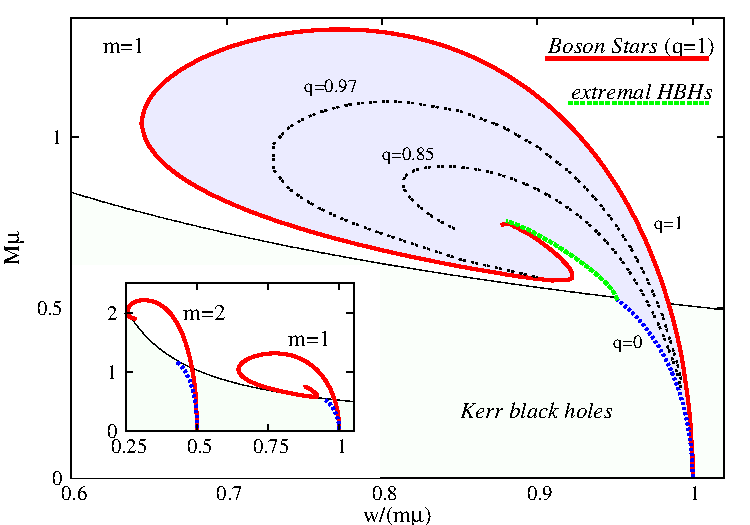
\includegraphics[width=0.497\textwidth]{BH-w-M}
     \includegraphics[width=0.497\textwidth]{zoom-w-M}
  \end{center}
  \caption{The $(\Omega_H,M)$ domain of existence for a sample of KNBHsUSH. (Main left panel) Diagram for $\Phi_H=0.3$ with the boson star envelope (red solid line), the existence line on the domain of KN BHs (blue dotted line) and the line of extremal KNBHsUSH (green dashed line). The black solid line corresponds to the extremal KN BHs; non-extremal solutions exist below. The black dotted lines have constant normalized Noether charge $q$. (Inset) diagram for $\Phi_H=0$, for comparison. (Right panel) Detail around the intersection of the existence lines with the extremal KNBHsUSH lines and the extremal KN lines for $\Phi_H=0,0.6$ and $0.8$.  
	}
  \label{fig:w-M}
\end{figure}
%%%%%%%%%%%%%%%%%%%%%%%%%%%%%%%%%%%%%%%%%%%%%%%%%%%%%%%%%%%
 
  
 In Fig.~\ref{fig:w-g} (left panel), we exhibit the ratio $ M^{\Psi}/M$, which gives another measure of hairiness
   as a function of $\Omega_H$,
for $\Phi_H=0.3$. The figure shows that small fractions of the total energy in the hair are only allowed for sufficiently large horizon angular velocity. When the angular velocity is small, equilibrium between the hair and the horizon is only possible for solutions with $q$ close to unity, $i.e.$, boson star-like. 
The inset in this figure shows the $(\Omega_H,Q_E)$ domain of existence of the KNBHsUSH solutions. It illustrates that the electric charge of the solutions, for fixed $\Omega_H$ between that of the Hod point and the maximum allowed frequency, $\Omega_H=\mu$, is maximized along the existence line (and in particular at the Hod point). But for lower values of the frequency, slightly larger charges than that found at the Hod point are possible, occurring along the extremal hairy BHs line.

 

 

%%%%%%%%%%%%%%%%%%%%%%%%%%%%%%%%%%%%%%
\subsubsection{Gyromagnetic ratio}
%%%%%%%%%%%%%%%%%%%%%%%%%%%%%%%%%%%%%%
Rotating charges give rise to a magnetic dipole moment, $\mu_M$. 
In classical electromagnetism, a generic relation of the form~\eqref{gyro}, 
between $\mu_M$ and the total angular momentum, mass and charge can be derived, 
for systems with constant ratio of charge to mass density, yielding $g=1$. 
When experiments such as that performed for Stern and Gerlach in the early XXth century, 
showed that the electron should have $g=2$, it became clear that a new fundamental description 
for the electron was necessary, beyond the scope of the non-relativistic quantum theory. 
Such a description appeared with the Dirac equation, which, from first principles predicts $g=2$, 
a value that is corrected by loop diagrams in Quantum Electrodynamics (QED), 
yielding the so called anomalous magnetic moment, whose agreement 
with experiment is one of the outstanding successes of QED.

In BH physics, Carter first observed that $g=2$ for the KN solution. 
Since then many other studies considered the gyromagnetic ratio of rotating charged BHs, 
for instance with different asymptotics and in higher dimensions (see $e.g.$~
\cite{Garfinkle:1990ib,Herdeiro:2000ap,Aliev:2004ec,Ortaggio:2006ng,Aliev:2006tt}). 
Here we show that the addition of scalar hair leads to a suppression of the gyromagnetic ratio, 
and of the corresponding magnetic dipole moment, 
with respect to that of a comparable KN BH.  
 A novel aspect is that $g$ 
can be smaller than 1, a rather unsual feature in other models of relativistic, 
charged and spinning compact objects, 
$cf.$~\cite{Novak:2003uj}. 


In Fig.~\ref{fig:w-g} (right panel), we exhibit the gyromagnetic ratio in a $(q,g)$-diagram, for KNBHsUSH with $\Phi_H=0.3$.
The diagram shows that the gyromagnetic ratio, $g$, of both the extremal and non-extremal hairy BH solutions, is always less than $2$.
As expected, it does approach $2$, for both cases, in the limit of vanishing hair.
Further insight is obtained by considering the quantity
\begin{eqnarray}
\Delta\equiv \frac{M^2}{Q_E^2+J^2/M^2} \ ,
\end{eqnarray}
which determines the KN bound $\Delta\geqslant 1$. Indeed, all KN BHs have $\Delta>1$. This bound is, however, violated by a large set of KNBHsUSH, in particular by those close to the BS limit. This is reminiscent of what has been found for KBHsSH - see the discussions in~\cite{Herdeiro:2014goa,Herdeiro:2015gia,Herdeiro:2015tia,Delgado:2016zxv}.  Our results show that
solutions with $g<1$ predominantly exhibit $\Delta<1$ and thus violate the KN bound -- $cf.$ the inset of Fig.~\ref{fig:w-g} (right panel).



%%%%%%%%%%%%%%%%%%%%%%%%%%%%%%%%%%%%%%%%%%%%
\begin{figure}[H]
  \begin{center}
    \includegraphics[width=0.497\textwidth]{Mpsi}
      \includegraphics[width=0.497\textwidth]{qg}
  \end{center}
  \caption{(Left panel) The ratio $M^\Psi/M$ is shown as a function of $\Omega_H$ for a sample of KNBHsUSH. The inset shows the electric charge as a function of $\Omega_H$, where the blue dotted line is the existence line. 
	(Right panel)  The $(q,g)$ space. The inset show $g$ as a function of $\Delta$, that determines the KN bound.
}
 \label{fig:w-g} 
\end{figure}
%%%%%%%%%%%%%%%%%%%%%%%%%%%%%%%%%%%%%%%%%%%%

 
 


%%%%%%%%%%%%%%%%%%%%%%%%%%%%%%%%%%%%%%%%%%%%
\section{Gauged scalar field model}
\label{sec_mod_g}
%%%%%%%%%%%%%%%%%%%%%%%%%%%%%%%%%%%%%%%%%%%%




%%%%%%%%%%%%%%%%%%%%%%%%%%%%%%%%
\subsection{Main differences in the model}

%%%%%%%%%%%%%%%%%%%%%%%%%%%%%%%%

Let us now consider the model described in Section~\ref{sec_mod_u} but with a \textit{gauged} scalar field, 
that couples minimally to the electromagnetic field, with gauge coupling $q_E$. 
This coupling is implemented by replacing the partial derivatives of the scalar field in the action~\eqref{action} as
\begin{equation}
\partial_a \Psi \longrightarrow D_a\Psi=\partial_a \Psi + iq_E A_a \Psi \ .
\label{mc}
\end{equation}
The Einstein equations still take the form~\eqref{eom}, but with the substitution~\eqref{mc} 
in the scalar field energy-momentum tensor~\eqref{emt}. Then, the scalar and Maxwell equations of motion become
\begin{eqnarray}
\label{field-eqs}
D_{a}D^{a}\Psi=\mu^2 \Psi\ , \qquad 
\nabla_{b}F^{ba}=
iq_E \big [ (D^{a}\Psi^*) \Psi-\Psi^*(D^a \Psi) \big ] 
\equiv q_E j^a  \ .
\end{eqnarray}  
Physically, the scalar field is now electrically charged 
(its quanta, the scalar particles, carry a charge $q_E$), and thus the scalar field sources the Maxwell field.

This model is invariant under the $local$ U(1) gauge transformation 
\begin{eqnarray}
\label{gauge-transf}
\Psi \to \Psi e^{-i q_E \alpha}\ ,~~A_a\to A_a+\partial_a \alpha \ ,
\end{eqnarray}
where $\alpha$ is a real function. One consequence of this gauge invariance is that the $(t, \varphi)$-dependence of the scalar field ansatz~\eqref{scalar_ansatz}, 
can now be gauged away by applying the local $U(1)$ symmetry
(\ref{gauge-transf})
with $\alpha =  (m\varphi -w t)/q_E$.  This, however, also changes the gauge field, as $A_t\to A_t-w/q_E$,
$A_\varphi \to A_\varphi+m/q_E$. 
%
Consequently, the solutions cannot be constructed starting with the configurations in the
previous sections and increasing $q_E$.
%
Thus, in order
to be able to consider this approach, we  keep the $(t,\varphi)$-dependence in 
the scalar field ansatz and fix the corresponding gauge freedom by setting $A_t = A_\varphi = 0$ at infinity.

One major difference with respect to the case 
discussed in the previous section 
 is that the solitonic limit of the solutions carries now a nonzero electric charge.
Self-gravitating charged boson stars were first considered, in spherical symmetry, in~\cite{Jetzer:1989av} 
(see also the recent work  \cite{Pugliese:2013gsa}). 
To the best of our knowledge, no rotating generalizations of these static solutions have been reported\footnote{ 
Some properties of the spinning charged solitons, 
with a self-interacting ($Q$-ball type) scalar field model, were addressed in~\cite{Brihaye:2009dx}.
}.
The Noether charge $Q$ of the solitons, $i.e.$ the total
particle number, is now intrinsically related to the electric charge $Q_E$. 
The former can be computed as  
%
\begin{eqnarray}
\label{Q1}
Q= \int j^t \sqrt{-g} dr  d\theta d\varphi=
 4\pi \int_{0}^\infty dr \int_0^\pi d\theta  
~r^2\sin \theta ~e^{-F_0+2F_1+F_2}  (w-q_E A_t -mW)\phi^2 \ ,
\end{eqnarray}
%
whereas the latter is read from the asymptotics
 of the electric potential $A_t$, as given in  (\ref{asym-matter-fields}). 
A straightforward computation 
shows that both the Noether charge and the electric charge of the spinning \textit{solitons}
are proportional  to the total angular momentum,
\begin{eqnarray}
\label{JQ}
J= m Q=\frac{4 \pi m Q_E}{q_E}\ .
\end{eqnarray} 


%%%%%%%%%%%%%%%%%%%%%%%%%%%%%%%%%%%%%%%%%%%%%%%%%%%%%%%%%%%%%%%%%%
\subsection{Features of the gauged scalar field solutions}
\label{sec_results_g}
%%%%%%%%%%%%%%%%%%%%%%%%%%%%%%%%%%%%%%%%%%%%%%%%%%%%%%%%%%%%%%%%%%
 
The construction of the  gauged scalar field solutions is similar 
to that described above for the ungauged case ($q_E=0$ limit).
In particular, the KNBHsGSH are subject to the same set of 
boundary conditions  used in the ungauged case.
The synchronization condition, however, is different,   
\begin{equation}
\label{cond-new}
 w-q_E \Phi_H=m \Omega_H \ ,
\end{equation}
in agreement with the result found in the linear theory~\cite{Hod:2014baa,Benone:2014ssa}.



The electrically charged boson stars also form a part of the domain of existence of KNBHsGSH. 
Thus we have paid special attention to this limiting case.
These solutions  are obtained by considering the ansatz~\eqref{metric_ansatz}--\eqref{electric_ansatz} with $r_H=0$ 
and replacing the boundary conditions at the horizon~\eqref{bch1} 
by the following boundary conditions at the origin
\begin{eqnarray}
\label{bc0} 
\partial_r F_i|_{r=0}= 
W|_{r=0}=0\ ,~~
\phi| _{r =0}=0\ ,~~\partial_r A_t|_{r=0}=A_\varphi|_{r=0}=0\ .
\end{eqnarray}
% 

Some results of the numerical integration are shown in Fig.~\ref{fig:w-M-gauged} (left panel).
The basic properties of the spinning gauged boson stars solutions can be summarized as follows.
First, for all values of the gauge coupling considered so far, 
the frequency dependence of the solutions is qualitatively similar to the ungauged case.
The solutions 
exist for a limited range of frequencies
$0<w_{min}<w<\mu$. 
In particular, we observe that the minimal frequency increases with $q_E$. 
After this minimal frequency, a backbending towards larger values of $w$ occurs, yielding a second branch of solutions. 
A second backbending, towards
smaller values of $w$,  is observed as the frequency reaches a maximal value along the second branch, $w\to w_{max}$, whose value increases again with $q_E$. 
Then, similarly to the ungauged limit, a third branch of solutions develops -- not shown in Fig.~\ref{fig:w-M-gauged} (left panel).
Subsequently, we expect the existence of an inspiraling behaviour of the solutions, 
in analogy with uncharged boson stars, towards a limiting configuration.  


%%%%%%%%%%%%%%%%%%%%%%%%%%%%%%%%%%%%%%%%%%%%%%%%%%%%%%%%%%%
\begin{figure}[H]
  \begin{center}
    \includegraphics[width=0.497\textwidth]{BS-w-M-gauged}
      \includegraphics[width=0.497\textwidth]{BS-g-M-gauged}
  \end{center}
  \caption{
	(Left panel)
	The $(w,M)$ diagram for spinning boson stars with $q_E=0$ (red curve), $q_E/\mu=0.2, 0.3, 0.4, 0.5$
	and $0.6$ (top curve).  
		(Right panel)
	The mass $M$ is shown as a function of the gauge coupling constant $q_E$
	for several frequencies, $w/\mu=0.7, 0.8, 0.9$ and $0.95$ (as an inset).	}
  \label{fig:w-M-gauged}
\end{figure}
 %%%%%%%%%%%%%%%%%%%%%%%%%%%%%%%%%%%%%%%%%%%%%%%%%%%%%%%%%%%
Although only the mass is displayed in Fig.~\ref{fig:w-M-gauged} (left panel), the $J(w)$
diagram has a very similar shape.
Consequently,  the axially symmetric gauged boson stars do not possess
a static limit.  Observe also that the maximal mass of spinning gauged boson stars solutions increases with $q_E$.


As shown in Fig.~\ref{fig:w-M-gauged} (right panel), 
the solutions possess also a nontrivial dependence on 
the gauge coupling constant $q_E$.
For given values of $w$,
spinning solutions exist up to a maximal
value of the gauge coupling constant only, $q_E=(q_E)_{max}$.
The physics rationale behind this behaviour 
is similar to that discussed for the spherically symmetric case 
\cite{Jetzer:1989av,Pugliese:2013gsa}.
For $q_E>(q_E)_{max}$ the charge repulsion  becomes bigger than
  the scalar and gravitational attraction and localized solutions cease to exist  
(note that the maximal value of $q_E$
increases with frequency).
Also, as seen in Fig.~\ref{fig:w-M-gauged} (right panel),
all global charges stay finite as $q_E\to (q_E)_{max}$.
 

KNBHsGSH are obtained by adding a horizon at the center of the spinning gauged boson star  
we have just described, which can be done for  any such  solution.
One way to construct the BHs
  is to  start from  boson stars 
and slightly increase the horizon size via the parameter $r_H$.
In this approach, the other input parameters 
$\Omega_H$, $q_E$,  $\Phi_H$ and $m$
are kept fixed. 
We recall that for BHs, the frequency $w$ is fixed by the synchronization condition (\ref{cond-new}).
Then one finds three 
possible behaviours for
the resulting branches of BH solutions -- see Fig.~\ref{fig:q-AH-gauged} (left panel).
 First  ($i$), for small enough values of $\Omega_H$,
 the branch of BHs connects two different boson stars; 
as $r_H\to 0$ the horizon area vanishes, $q\to 1$, while the temperature
 diverges.
For intermediate values of  $\Omega_H$,
the branch of solutions ends in an extremal KNBHsGSH solution ($ii$). 
These limiting configurations have finite
horizon size   and global charges, $0<q<1$ and appear to possess 
a regular horizon.
Finally   ($iii$), for large values of $\Omega_H$,
the branch of  KNBHsGSH interpolates between 
a charged boson star and a set of critical KN solutions (with $q=0$ and $A_H>0$), which lies again 
on an {\it existence line}. 

 In Fig.~\ref{fig:q-AH-gauged} (right panel) we exhibit the (Komar) energy density and angular momentum density (in the inset) for an illustrative example of a KNBHGSH  with physical input parameters 
$r_H=0.24, w =0.86, q_E =0.2, \Phi_H=0.1$. 
These densities have a contribution from both the electromagnetic and the scalar field. The main feature we wish to emphasize is the composite structure revealed by the plots. KN BHs have an (electromagnetic) energy and angular momentum density that decays with the radial coordinate, whereas KBHsSH 
(and boson stars)
have toroidal-like distributions for the (scalar) energy and angular momentum densities. 
Consequently, KNBHsGSH exhibit a superposition of these two behaviours, with decaying densities from the horizon but which exhibit a local maximum, in the neighbourhood of the equatorial plane, at some finite radial coordinate. 
A similar energy and angular momentum distribution can be found for KNBHsUSH.  

The behaviours illustrated in Fig.~\ref{fig:q-AH-gauged} supports the expectation that the domain of existence of KNBHsGSH will fill in the domain delimited by the boson star curves exhibited in Fig.~\ref{fig:w-M-gauged} (left panel), together with the existence line of KN BHs and a line of extremal KNBHsGSH,  in a qualitatively similar fashion to that shown in Fig.~\ref{fig:w-M} (left panel). Having established these solutions exist, and that their domain of existence will be analogue to the case of KNBHsUSH, we will not enter further details here; its systematic and detailed study will be reported elsewhere.
Here we mention only that, similar to the ungauged case, 
the gyromagnetic ratio of  KNBHsGSH constructed so far is always smaller than $g=2$.


%%%%%%%%%%%%%%%%%%%%%%%%%%%%%%%%%%%%%%%%%%%%%%%%%%%%%%%%%%%
\begin{figure}[H]
  \begin{center}
    \includegraphics[width=0.497\textwidth]{BH-q-AH} 
      \includegraphics[width=0.497\textwidth]{energy-2d} 
  \end{center}
  \caption{ (Left panel) 
	The $(A_H,q)$ diagram is shown for three sets of KNBHsGSH solutions with fixed values of 
$\Omega_H$ and 
$q_E/\mu=0.2$, 
$\Phi_H=0.1$. (Right panel) 
 Energy density (and angular momentum density in the inset) along three different slices of constant $\theta$ for an illustrative example of a KNBHGSH.
	}
  \label{fig:q-AH-gauged}
\end{figure}
 %%%%%%%%%%%%%%%%%%%%%%%%%%%%%%%%%%%%%%%%%%%%%%%%%%%%%%%%%%%
 


%%%%%%%%%%%%%%%%%%%%%%
\section{Remarks}
\label{sec_remarks}
%%%%%%%%%%%%%%%%%%%%%%%

The Kerr solution~\cite{Kerr:1963ud}, which describes the paradigmatic BH geometry in General Relativity, allows a generalization with electric (or magnetic) charge~\cite{Newman:1965my}, discovered shortly after the Kerr metric. Much more recently, it was found that the Kerr solution also allows a generalizations with scalar~\cite{Herdeiro:2014goa,Herdeiro:2015gia,Kleihaus:2015iea,Herdeiro:2015tia,Chodosh:2015oma} or Proca hair~\cite{Herdeiro:2016tmi}. The former are known as Kerr BHs with scalar hair (KBHsSH). In this paper we have added electric charge to KBHsSH, both considering an ungauged and a gauged scalar field and analysed some basic properties of the solutions. In both cases, their domain of existence is qualitatively similar to the of the uncharged hairy BHs. In particular it is bounded by three curves, corresponding do the solitonic limit (boson stars), extremal hairy BHs, and bald (KN) BHs. In the gauged case, the solitonic limit corresponds to rotating charged boson stars, which hitherto have not been studied in the literature. 

As an example of a novel physical property of these solutions we have considered the gyromagnetic ratio, $g$. This quantity measures how a magnetic dipole moment is induced by the charge and angular momentum of the BH. It is well known the relativistic (Dirac) value holds for the KN BH, $g=2$~\cite{Carter:1968rr}. We have shown that the gyromagnetic ratio of these hairy charged BHs is always $g\leqslant 2$, with equality attained only in the ``bald" case. Thus, the scalar hair leads to a suppression of the magnetic dipole moment. Preliminary work (not reported herein), analysing the electromagnetic field lines of the BHs, suggests that the scalar hair also suppresses the higher electric multipole moments. We hope to give a detailed account of this behaviour in the near future.




There are other interesting applications for these solutions. As an example we mention testing the no-short hair conjecture. As originally stated~\cite{Nunez:1996xv}, this conjecture suggested that, when hair exists around a spherically symmetric BH, the `hair' should extend
beyond $3r_+/2$, where $r_+$ is the areal radius of the event horizon. This radius coincides with the location of the
circular null geodesic for the Schwarzschild solution, which led to an improved version of the conjecture that the hair must extend beyond the null circular orbit of the spacetime~\cite{Hod:2011aa}. For rotating BHs, an analysis of linearized hair suggested the no-short hair conjecture holds for uncharged BHs~\cite{Hod:2016dkn}, but may be violated for electrically charged ones~\cite{Hod:2014sha,Hod:2015ynd}. The latter possibility can be tested using the fully non-linear solutions of the Einstein-Maxwell-Klein-Gordon field equations reported in this paper. 








%%%%%%%%%%%%%%%%%%%%%%%%%%%%%%%%%%%%%%%%%%%%%%%%%%%%%%%%%%%%%%%%%%%%%%%%%%%%%%
\section*{Acknowledgements}
%%%%%%%%%%%%%%%%%%%%%%%%%%%%%%%%%%%%%%%%%%%%%%%%%%%%%%%%%%%%%%%%%%%%%%%%%%%%%%
C. H. and E. R. acknowledge funding from the FCT-IF programme. H.R. is supported by the grant PD/BD/109532/2015 under the MAP-Fis Ph.D. programme. This  work  was  partially  supported  by  the  H2020-MSCA-RISE-2015  Grant  No. StronGrHEP-690904,  and  by  the  CIDMA  project  UID/MAT/04106/2013.  Computations were performed at the BLAFIS cluster, in Aveiro University.

\bigskip










\bibliography{bibtex_calculation}
\bibliographystyle{h-physrev4}

\end{document}% v2: 13 August 13
% v5: 15 Oct 13
%
 \documentclass{article}


\usepackage{epsfig} 
\usepackage{amsmath}
\usepackage{amsfonts}
\usepackage{graphicx}
%\usepackage{mathtools}
\usepackage{cite}
%\usepackage{tipa}

 

 \usepackage{amssymb}

\tolerance=10000
\pagenumbering{arabic}
\textheight 22.cm
\textwidth 16.5 cm
\oddsidemargin 0.5cm\evensidemargin 0.5cm
\topmargin=-1.cm
\hoffset -0.5cm
\date{\today} 
 
\newcommand{\bnabla}{\mbox{\boldmath $\nabla$}}
%\newcommand{\bomega}{\mbox{\boldmath $\omega$}}
\newcommand{\bOmega}{\mbox{\boldmath $\Omega$}}

\newcommand{\insertplot}[5]{\begin{figure}
 \hfill\hbox to 0.05in{\vbox to #5in{\vfill
 \inputplot{#1}{#4}{#5}}\hfill}
 \hfill\vspace{-.1in}
 \caption{#2}\label{#3}
 \end{figure}}
 \newcommand{\inputplot}[3]{\special{ps:: gsave #2 -36 mul 0 rmoveto
   currentpoint translate #2 7.0 div #3 5.0 div scale}
 \special{ps: plotfile #1}\special{ps:: grestore}}
\newcounter{fig}   \newcommand{\lbfig}[1]{\refstepcounter{fig}
\label{#1} }

\numberwithin{equation}{section}
 
\newcommand{\vphi}{\varphi}
\newcommand{\DS}{\displaystyle}
\newcommand{\pih}{\frac{\pi}{2}}
\newcommand{\sqdetg}{\sqrt{-g}}
\newcommand{\sqdetgi}{\frac{1}{\sqrt{-g}}}
\newcommand{\edil}{e^{2\kappa \phi}}
\newcommand{\bA}{\bar{A}}
\newcommand{\bF}{\bar{F}}
\newcommand{\bD}{\bar{D}}

\renewcommand{\a}{\alpha}
\renewcommand{\b}{\beta}
\renewcommand{\c}{\gamma}
\renewcommand{\d}{\delta}  
\newcommand{\g}{\nu}
\renewcommand{\l}{\lambda}
\renewcommand{\t}{\theta}
\newcommand{\rot}{\mbox{rot}}
\renewcommand{\div}{\mbox{div}}
\newcommand{\cosec}{\mbox{cosec}}

 

\newcommand{\ta}{\theta}
\newcommand{\Si}{\Sigma}
\newcommand{\vf}{\varphi}
\newcommand{\dd}{\mbox{d}}
\newcommand{\tr}{\mbox{tr}}
\newcommand{\la}{\lambda}
\newcommand{\ka}{\kappa}
\newcommand{\f}{\phi}
\newcommand{\al}{\alpha}
\newcommand{\ga}{\gamma}
\newcommand{\de}{\delta}
\newcommand{\si}{\sigma}
\newcommand{\bomega}{\mbox{\boldmath $\omega$}}
\newcommand{\bsi}{\mbox{\boldmath $\sigma$}}
\newcommand{\bchi}{\mbox{\boldmath $\chi$}}
\newcommand{\bal}{\mbox{\boldmath $\alpha$}}
\newcommand{\bpsi}{\mbox{\boldmath $\psi$}}
\newcommand{\brho}{\mbox{\boldmath $\varrho$}}
\newcommand{\beps}{\mbox{\boldmath $\varepsilon$}}
\newcommand{\bxi}{\mbox{\boldmath $\xi$}}
\newcommand{\bbeta}{\mbox{\boldmath $\beta$}}
\newcommand{\ee}{\end{equation}}
\newcommand{\eea}{\end{eqnarray}}
\newcommand{\be}{\begin{equation}}
\newcommand{\bea}{\begin{eqnarray}}

\newcommand{\ii}{\mbox{i}}
\newcommand{\e}{\mbox{e}}
\newcommand{\pa}{\partial}
\newcommand{\Om}{\Omega}
\newcommand{\vep}{\varepsilon}
%\newcommand{\bfR}{{\bf R}}
\newcommand{\bfph}{{\bf \phi}}
\newcommand{\lm}{\lambda}
\def\theequation{\arabic{equation}}
%\topmargin= -02cm\textheight= 23.cm\textwidth= 16.cm
%\oddsidemargin=-01cm\evensidemargin=-01cm \font\sqi=cmssq8
\renewcommand{\thefootnote}{\fnsymbol{footnote}}
\newcommand{\re}[1]{(\ref{#1})}
\newcommand{\R}{{\rm I \hspace{-0.52ex} R}}
\newcommand{\N}{{\sf N\hspace*{-1.0ex}\rule{0.15ex}%
{1.3ex}\hspace*{1.0ex}}}
\newcommand{\Q}{{\sf Q\hspace*{-1.1ex}\rule{0.15ex}%
{1.5ex}\hspace*{1.1ex}}}
\newcommand{\C}{{\sf C\hspace*{-0.9ex}\rule{0.15ex}%
{1.3ex}\hspace*{0.9ex}}}
\newcommand{\eins}{1\hspace{-0.56ex}{\rm I}}
\renewcommand{\thefootnote}{\arabic{footnote}}

\def\theequation{\thesection.\arabic{equation}}



\begin{document}

%%%%%%%%%%%%%%%%%
%%%   TITLE   %%%
%%%%%%%%%%%%%%%%%




\title{\bf \Large Kerr black holes with Proca hair}

 \author{
{\large Carlos Herdeiro}\footnote{herdeiro@ua.pt}, \
{\large Eugen Radu}\footnote{eugen.radu@ua.pt} \
and
{\large Helgi R\'unarsson}\footnote{helgi.runarsson@gmail.com}
\\ 
\\
{\small Departamento de F\'\i sica da Universidade de Aveiro and} \\ 
{\small Center for Research and Development in Mathematics and Applications (CIDMA)} \\ 
{\small   Campus de Santiago, 3810-183 Aveiro, Portugal}
}


 
 
%%%%%%%%%%%%%%%%
%%%   DATE   %%%
%%%%%%%%%%%%%%%%

\date{March 2016}
\maketitle

%%%%%%%%%%%%%%%%%%%%
%%%   ABSTRACT   %%%
%%%%%%%%%%%%%%%%%%%%
\begin{abstract}
Bekenstein proved that in Einstein's gravity minimally coupled to one (or many) real, Abelian, Proca field, stationary black holes (BHs) cannot have Proca hair. Dropping Bekenstein's assumption that matter inherits spacetime symmetries, we show this model admits asymptotically flat, stationary, axi-symmetric, regular on and outside an event horizon BHs with Proca hair, for an even number of real  (or an arbitrary number of complex) Proca fields. To establish it, we start by showing that a test, complex Proca field can form bound states, with real frequency, around Kerr BHs: \textit{stationary Proca  clouds}. These states exist at the threshold of superradiance.  It was conjectured in~\cite{Herdeiro:2014goa,Herdeiro:2014ima}, that the existence of such clouds at the linear level implies the existence of a new family of BH solutions at the non-linear level. We confirm this expectation and explicitly construct examples of such \textit{Kerr black holes with Proca hair} (KBHsPH). For a single complex Proca field, these  BHs form a countable number of families with three continuous parameters (ADM mass, ADM angular momentum and Noether charge). They branch off from the Kerr solutions that can support stationary Proca clouds and reduce to Proca stars~\cite{Brito:2015pxa} when the horizon size vanishes. We present the domain of existence of one family of KBHsPH, as well as its phase space in terms of ADM quantities. Some physical properties of the solutions are discussed; in particular, and in contrast with Kerr BHs with scalar hair, some spacetime regions can be counter-rotating with respect to the horizon. 
We further establish a no-Proca-hair theorem for static, spherically symmetric BHs but allowing the complex Proca field to have a harmonic time dependence, which shows BHs with Proca hair in this model require rotation and have no static limit. KBHsPH are also disconnected from Kerr-Newman BHs with a real, massless vector field.

\end{abstract}


%%%%%%%%%%%%%%%%
%%%   PACS   %%%
%%%%%%%%%%%%%%%%

%\pacs{
%04.20.Jb 	%Exact solutions
%04.40.-b 	%Self-gravitating systems; continuous media and classical fields in curved spacetime
%04.70.-s 	%Physics of black holes
%}


%%%%%%%%%%%%%%%%%%%%%%
%%%   MAKE TITLE   %%%
%%%%%%%%%%%%%%%%%%%%%%


%%%%%%%%%%%%%%%%%%%%%%%%%%%%%%%%%%%%%%%%%%%%%%%%%%%%%%%%%%%%%%%%%%%%%



%\tableofcontents
 
 \newpage

%%%%%%%%%%%%%%%%%%%%%%%%%%%%%%%%%%%%%%%%%%%%%%%%%%%%%%%%%%%%%%%%%%%%%%%%%%%%%%%
\section{Introduction}
%%%%%%%%%%%%%%%%%%%%%%%%%%%%%%%%%%%%%%%%%%%%%%%%%%%%%%%%%%%%%%%%%%%%%%%%%%%%%%%
 
In vacuum General Relativity (GR) black holes (BH) are remarkably simple. The Carter-Robinson theorem~\cite{Carter:1971zc,Robinson:1975bv}, supplemented by the rigidity theorem~\cite{Hawking:1971vc,Racz:1995nh}, established that asymptotically flat, stationary, non-singular (on and outside an event horizon)  \textit{vacuum} BHs of GR have \textit{only} 
two degrees of freedom -- see~\cite{Chrusciel:2012jk} for a review.  

The most general BH solution in this context is the Kerr metric~\cite{Kerr:1963ud} and the two degrees of freedom are the ADM mass, $M$, and angular momentum, $J$, both of which can be determined by an observer at infinity. 

The natural question of how this result generalizes in the presence of matter led to the \textit{no-hair} hypothesis~\cite{Ruffini:1971bza}: regardless of the matter involved, the end-point of gravitational collapse -- in GR and in an astrophysical context -- is characterized solely by conserved charges associated to Gauss laws, including $M,J$, and no further parameters (\textit{hair}). Thus, an observer at infinity should be able to fully compute all relevant ``charges" of an equilibrium BH.

Evidence in favour of this hypothesis has been presented in terms of \textit{no-hair theorems} for particular matter models in GR. A collection of such theorems for the much studied case of scalar matter can be found in the recent review~\cite{Herdeiro:2015waa}. Of relevance for the present paper, Bekenstein established a no-Proca hair theorem for stationary BH solutions of Einstein's gravity minimally coupled to one (or more) real, Abelian Proca field~\cite{Bekenstein:1971hc,Bekenstein:1972ky}, which will be reviewed in Section~\ref{sec_nohair1}. 



Evidence against the no-hair hypothesis in asymptotically flat spacetimes, on the other hand, has been presented in the form of hairy BH solutions, starting with the pioneering examples in Yang-Mills theory~\cite{Volkov:1998cc} (see also the reviews~\cite{Bizon:1994dh,Bekenstein:1996pn,Herdeiro:2015waa,Volkov:2016ehx}). 
Such counter-examples, however, typically either 
1) violate some energy condition ($e.g.$~\cite{Nucamendi:1995ex,Bechmann:1995sa,Anabalon:2013qua,Anabalon:2012ih,Cadoni:2015gfa}); or 
2) have non-minimal couplings between matter and geometry ($e.g.$~\cite{Bekenstein:1975ts,Bekenstein:1974sf,BBM,Sotiriou:2014pfa,Sotiriou:2013qea,Babichev:2013cya}); or 
3) have non-canonical/non-linear kinetic terms ($e.g.$~\cite{Luckock:1986tr,Luckock,Bronnikov:2005gm,Radu:2011uj}); or 
4) the hair is not independent of other fields, such as an electromagnetic field (secondary hair, $e.g.$~\cite{Gibbons:1987ps,Gibbons:1982ih}); or 
5) involve higher curvature terms 
($e.g$~\cite{Kanti:1995vq,Ayzenberg:2014aka,Kleihaus:2011tg,Kleihaus:2015aje,Pani:2011gy,Pani:2009wy,Alexander:2009tp,Yunes:2009hc}); or 
6) several of the above. It is unclear, moreover, if any of these counter-examples violates the \textit{dynamical spirit} of the no-hair hypothesis; that is, if there are dynamically stable hairy BHs that can be the end-point (or be sufficiently long lived) in a dynamical evolution.

\bigskip

In a qualitatively novel development, a class of BH solutions with scalar hair was found in 2014 bifurcating from the Kerr metric~\cite{Herdeiro:2014goa}: \textit{Kerr BHs with scalar hair} (KBHsSH).
%
 These are solutions of the simple model
 \begin{equation}
\label{actionscalar}
S=\int  d^4x \sqrt{-g}\left[ \frac{R}{16\pi G}
   -\frac{g^{\alpha\beta}}{2} \left( \Psi_{, \, \alpha}^* \Psi_{, \, \beta} + \Psi _
{, \, \beta}^* \Psi _{, \, \alpha} \right) - \mu^2 \Psi^*\Psi
%( \left| \Phi \right|) 
 \right]  \ ,
\end{equation}
that 1) obey all energy conditions; 2) have minimal couplings with the geometry; 3) have canonical kinetic terms; 4) have an independent (primary) hair; 5) exist in GR, without higher curvature terms. KBHsSH, moreover, are asymptotically flat, regular on and outside the event horizon, reduce to (specific) Kerr solutions in the limit of vanishing hair, and to gravitating solitons known as \textit{boson stars}~\cite{Schunck:2003kk,Liebling:2012fv} in the limit of vanishing horizon. The scalar hair is described by an independent  conserved Noether charge \textit{but without} an associated Gauss law. Thus, an observer at infinity cannot determine this charge -- which must be computed by a volume integral -- and hence does not have access to all the relevant spacetime charges.  

The matter content for the original example in~\cite{Herdeiro:2014goa} (see also~\cite{Herdeiro:2015gia}) was a massive complex scalar field, $cf.$~\eqref{actionscalar}. In GR minimally coupled to this type of matter the Kerr BH is a solution, together with a vanishing scalar field, but it is \textit{unstable} against superradiance~\cite{Press:1972zz,Damour:1976kh,Brito:2015oca}. At the threshold of the instability, there are bound states of the scalar field on the Kerr background, found in a test field analysis, corresponding to linear hair. The existence of these \textit{stationary scalar clouds}~\cite{Hod:2012px,Hod:2013zza,Herdeiro:2014goa,Hod:2014baa,Benone:2014ssa,Hod:2014npa,Hod:2015ota} determines the bifurcation point of the hairy solutions from vacuum Kerr. Moreover, since the latter solution is unstable against superradiant scalar perturbations, there is an expectation that the BHs of~\cite{Herdeiro:2014goa} play a role in the non-linear development of the instability and can effectively form dynamically, thus providing a true counter-example to the physical implications of the no-hair hypothesis -- see~\cite{Sanchis-Gual:2015lje,Bosch:2016vcp} for recent discussions of the non-linear development of superradiant instabilities into hairy BHs. 

\bigskip

The connection between KBHsSH and superradiance led to the suggestion that, underlying the example of KBHsSH, there is a more general mechanism~\cite{Herdeiro:2014goa,Herdeiro:2014ima} (see also~\cite{Herdeiro:2015waa,Herdeiro:2015gia}): 
\newpage
{\bf Conjecture:}
\begin{description}
\item[1)] If a ``hairless" stationary BH spacetime $(\mathcal{M}_0,{\bf g_0})$ is afflicted by superradiant instabilities triggered by a given test field $\mathcal{F}$;
\item[2)] If the field modes at the threshold of the instability (zero modes), $\mathcal{F}_t$, yield an energy-momentum tensor $\mathcal{T}(\mathcal{F}_t,\mathcal{F}_t)$ which is time-independent $\mathcal{L}_{\bf k}\mathcal{T}(\mathcal{F}_t,\mathcal{F}_t)=0$, where ${\bf k}$ is the time-like Killing vector field (at infinity) that preserves the metric $\mathcal{L}_{\bf k}{\bf g_0}=0$;
\item[Then:] there is a new family of stationary BH ``hairy solutions" bifurcating from $(\mathcal{M}_0,{\bf g_0})$, denoted by $(\mathcal{M}_\mathcal{F},{\bf g_\mathcal{F}})$. Actually, $(\mathcal{M}_\mathcal{F},{\bf g_\mathcal{F}})$ may be a countable set of families.
\end{description}
In the case of KBHsSH, one encounters a family with three continuous and two discrete degrees of freedom. The former are the ADM mass and angular momentum $(M,J)$ and the Noether charge $Q$; the latter, which define a countable set of families, are the node number, $n\in \mathbb{N}_0$ and the azimuthal harmonic index, $m\in \mathbb{Z}$ of the scalar field. A formal proof of the existence of these solutions was recently reported in~\cite{Chodosh:2015oma}. KBHsSH were generalized to include self-interactions of the scalar field in~\cite{Herdeiro:2015tia} and to scalar-tensor gravity in~\cite{Kleihaus:2015iea}.

\bigskip

As further evidence for the above conjecture we consider, in this paper, 
Einstein's gravity minimally coupled to Abelian Proca fields, hereafter referred simply as Proca fields\footnote{Gravitating \textit{non-Abelian} ($SU(2)$) Proca fields have been studied in \cite{Greene:1992fw}, wherein spherically symmetric solitons and BHs have been discussed. The properties of these solutions are rather distinct from the solutions discussed in this paper and, moreover, the former have not been generalized to include rotation.}. 
Massive Proca fields trigger, in much the same way as massive scalar fields, 
superradiant instabilities of Kerr BHs -- see~\cite{Pani:2012vp,Pani:2012bp,Witek:2012tr} 
for recent studies of Proca-induced superradiant instabilities in asymptotically flat BHs. 
Firstly, we shall perform a test field analysis of a Proca field on the Kerr background. We observe that, at the threshold of the unstable modes, one can find \textit{stationary Proca clouds}. 
If the Proca field is complex, moreover, the energy-momentum tensor sourced by these stationary clouds is time-independent. Hence, we are in the conditions of the above conjecture. Secondly, we address the fully non-linear system of a complex-Proca field minimally coupled to GR and construct stationary BH solutions which are the non-linear realization of the aforementioned stationary Proca clouds: \textit{Kerr BHs with Proca hair} (KBHsPH). When the horizon of these BHs vanishes, the solutions reduce to the rotating Proca stars recently constructed in~\cite{Brito:2015pxa}. These are vector boson stars which share many of the properties of the scalar boson stars that have been studied for decades~\cite{Schunck:2003kk,Liebling:2012fv}.

\bigskip

The introduction of the mass term for the vector fields is central for the existence of KBHsPH, since it is crucial for both the existence of the stationary Proca clouds and Proca stars. In the (Proca field) massless limit these BHs trivialize; they are not connected to Kerr-Newman BHs. The presence of such mass terms implies that there is no Gauss law associated to the vector field;  massive fields have no Gauss law since there is no flux conservation. Indeed, in asymptotically flat spacetimes, a massive field which decays towards spatial infinity will do so exponentially. Thus, the integral of its flux density over a sphere at infinity will necessarily vanish. 

This does not mean, however, that massive fields cannot be \textit{locally} conserved. Both the complex Proca field and the complex, massive scalar field enjoy a $U(1)$ global symmetry which implies a conserved current and a conserved Noether charge. There is a local continuity equation, but no Gauss law. Thus, according to the no-hair hypothesis there should be no Proca hair around stationary BHs. Here, however, we show that there can be. And again, an observer at infinity does not have access to all relevant spacetime charges.

\bigskip

This paper is organized as follows. In Section~\ref{sec_model} we exhibit the Einstein--complex-Proca model and its basic properties. In Section~\ref{sec_nohair} we review the classic no-Proca-hair theorem by Bekenstein~\cite{Bekenstein:1971hc,Bekenstein:1972ky} and also present a novel no-Proca-hair theorem applying to \textit{spherically symmetric} solutions and allowing the Proca field to have a harmonic time dependence. The latter is a generalization of the theorem presented in~\cite{Pena:1997cy} for the scalar case and it establishes that rotation is crucial for the existence of KBHsPH. In Section~\ref{sec_clouds} we consider the construction of stationary Proca clouds around Kerr and obtain one existence line for a particular set of ``quantum" numbers. In Section~\ref{sec_stars} we shall briefly review some of the main features of Proca stars, that form a limiting case of KBHsPH, and discuss some of their physical properties in the rotating case. In Section~\ref{sec_kbhsph} we finally construct KBHsPH, discussing the ansatz, boundary conditions and solving numerically the field equations. Then we exhibit the domain of existence and phase space of one family of solutions, we discuss the Proca energy spacetime distribution and some other physical features of these BHs. We close with a discussion of the results of this paper and some of the open directions for future related research.  In the Appendices we provide some technical results, including the explicit expression for the Einstein tensor, Proca energy-momentum tensor and Proca field equations.







 %%%%%%%%%%%%%%%%%%%%%%%%%%%%%%%%%%%%%%%%%%%%%%%%%%%%%%%%%%%%%%%%%%%%%%%%%%%%%%%
\section{Einstein--complex-Proca model}
\label{sec_model}
%%%%%%%%%%%%%%%%%%%%%%%%%%%%%%%%%%%%%%%%%%%%%%%%%%%%%%%%%%%%%%%%%%%%%%%%%%%%%%% 
The field equations for a massive vector field were introduced by A. Proca~\cite{Proca} in the 1930s. Much more recently, gravitating Proca fields have been discussed by various authors -- see $e.g.$~\cite{Rosen:1994rq,Obukhov:1999ed,Toussaint:1999zz}. Here, we shall consider  two real Proca fields, both with mass $\mu$, but our discussion can be easily generalized to an arbitrary even number of real Proca fields (or an arbitrary number of complex ones). 
The two fields are described by the potential 1-forms $A^{(i)}$, $i=1,2$, and field strengths $F^{(i)}=dA^{(i)}$. It is convenient to organize them into a single complex Proca field:
\begin{equation}
\mathcal{A}=A^{(1)}+iA^{(2)} \ , \qquad \mathcal{F}=F^{(1)}+iF^{(2)} \ .
\end{equation}
We denote the complex conjugate by an overbar,
\begin{equation}
\bar{\mathcal{A}}=A^{(1)}-iA^{(2)} \ , \qquad \bar{\mathcal{F}}=F^{(1)}-iF^{(2)} \ .
\end{equation}
Considering that the two Proca fields do not couple to each other and couple minimally to gravity, one obtains the minimal Einstein--complex-Proca model, which is  
described by the action:
\begin{equation}
\label{action}
\mathcal{S}=\int d^4x \sqrt{-g}\left(\frac{1}{16 \pi  G}R
-\frac{1}{4}\mathcal{F}_{\alpha\beta}\bar{\mathcal{F}}^{\alpha\beta}
-\frac{1}{2}\mu^2\mathcal{A}_\alpha\bar{\mathcal{A}}^\alpha\right) \ .
\end{equation}
This (or its version with $A_\alpha$ real) 
is the action considered by previous studies of the Einstein-Proca model, see
$e.g.$ refs. \cite{Rosen:1994rq,Vuille:2002qz}.\footnote{We remark that these works did not succeed in finding regular particle-like solutions or BHs with Proca hair.}



Varying  (\ref{action}) $w.r.t.$ the potential $A_\alpha$ yields the Proca field equations
\begin{equation}
\nabla_\alpha\mathcal{F}^{\alpha\beta}=\mu^2 \mathcal{A}^\beta \ .
\label{procafe}
\end{equation}
Observe that these equations \textit{completely} determine $ \mathcal{A}^\beta$ once $\mathcal{F}^{\alpha\beta}$ is known. Thus, the Proca potential is not subject to gauge transformations, unlike the Maxwell potential, and it is as physical as the field strength. In particular \eqref{procafe} imply the Lorentz condition, thus a dynamical requirement, rather than a gauge choice:
\begin{equation}
\nabla_\alpha\mathcal{A}^\alpha = 0 \ .
\label{lorentz}
\end{equation}


As usual, the Einstein equations are found by taking the variation of
(\ref{action}) $w.r.t.$ the metric tensor $g_{\alpha \beta}$
\begin{equation}
R_{\alpha \beta}-\frac{1}{2}R g_{\alpha \beta}=8 \pi G T_{\alpha \beta} \ ,
\label{Einstein-eqs}
\end{equation}
where the energy-momentum tensor reads:
\begin{eqnarray}
T_{\alpha\beta}=\frac{1}{2}
( \mathcal{F}_{\alpha \sigma }\bar{\mathcal{F}}_{\beta \gamma}
+\bar{\mathcal{F}}_{\alpha \sigma } \mathcal{F}_{\beta \gamma}
)g^{\sigma \gamma}
-\frac{1}{4}g_{\alpha\beta}\mathcal{F}_{\sigma\tau}\bar{\mathcal{F}}^{\sigma\tau}+\frac{1}{2}\mu^2\left[  
\mathcal{A}_{\alpha}\bar{\mathcal{A}}_{\beta}
+\bar{\mathcal{A}}_{\alpha}\mathcal{A}_{\beta}
-g_{\alpha\beta} \mathcal{A}_\sigma\bar{\mathcal{A}}^\sigma\right]\ . \ \ \ \ \ \ \  \ 
\label{procaemt}
\end{eqnarray}

The action possesses a global $U(1)$ symmetry, since it is invariant under the transformation 
$\mathcal{A}_\beta\rightarrow e^{i\chi}\mathcal{A}_\beta$, with $\chi$ constant; 
this implies the existence of a  4-current, 
%
\begin{equation}
\label{j}
j^\alpha=\frac{i}{2}\left[\bar{\mathcal{F}}^{\alpha \beta}\mathcal{A}_\beta-\mathcal{F}^{\alpha\beta}\bar{\mathcal{A}}_\beta\right] \ ,
\end{equation}
which is conserved by virtue of the field equations (\ref{procafe}): $\nabla_\alpha j^\alpha=0$. Consequently, there exists a Noether charge, $Q$, obtained integrating the temporal component of the 4-current on a space-like slice $\Sigma$:
\begin{equation}
Q=\int_\Sigma d^3x j^0 \ .
\label{q}
\end{equation}
We emphasize that unlike the massless limit of the theory, wherein the global symmetry becomes local, the last integral cannot be converted into a surface integral. In other words, there is no Gauss law.


 
 %%%%%%%%%%%%%%%%%%%%%%%%%%%%%%%%%%%%%%%%%%%%%%%%%%%%%%%%%%%%%%%%%%%%%%%%%%%%%%%
\section{No Proca-hair theorems}
\label{sec_nohair}
%%%%%%%%%%%%%%%%%%%%%%%%%%%%%%%%%%%%%%%%%%%%%%%%%%%%%%%%%%%%%%%%%%%%%%%%%%%%
If one considers Maxwell's equations for a test field with a spherically symmetric ansatz (a purely radial electric field) on the Schwarzschild background one finds a regular solution on and outside the Schwarzschild horizon ($cf.$ Section 2.1 in~\cite{Herdeiro:2015waa}). This is a smoking gun that a spherically symmetric field can be added, non-linearly, to the Schwarzschild solution, which indeed yields the well-known Reissner-Nordstr\"om BH. 
Adding a mass term to the Maxwell field -- hence converting it into a Proca field -- drastically alters the behaviour of the test field solution: it is not possible to find a solution which is both finite at the horizon and at spatial infinity, no matter how small $\mu$ is. 
In particular, for the asymptotically (exponentially) decaying solution, the Proca potential squared diverges at the horizon~\cite{Gottlieb:1984jg} - see Section~\ref{sec_nohair2}. Thus, requiring any amount of Proca field in equilibrium outside the horizon implies an infinite pile up of Proca invariants at the horizon. This behaviour parallels that of a scalar field (massless or massive) discussed in~\cite{Herdeiro:2015waa} and it is intimately connected with the existence/absence of a Gauss law for the Maxwell/Proca field. Moreover, it shows one cannot find a regular, spherically symmetric BH solution with Proca (time-independent) hair bifurcating from the Schwarzschild solution.

We shall review in~Section \ref{sec_nohair1} a more robust argument for the inexistence of stationary BHs with Proca hair, due to Bekenstein~\cite{Bekenstein:1971hc,Bekenstein:1972ky}, and that applies to our model~\eqref{action}. A fundamental assumption in the argument is that the Proca field and the background share the same symmetries. This \textit{symmetry inheritance} of the spacetime symmetries by the matter fields is precisely the assumption that  the KBHsPH presented later in this paper will violate. Then, in Section \ref{sec_nohair2}, we show that even dropping the symmetry inheritance assumption one can establish a no-hair theorem, for \textit{spherically symmetric} BHs. This is compatible with the KBHsPH solutions presented here, which are stationary and axi-symmetric, and shows that these solutions cannot have a static limit. This fact is in agreement with the domain of existence of KBHsPH, $cf.$ Section~\ref{subsec_III}.


%%%%%%%%%%%%%%%%%%%%%%%%%%%%%%%%%%%
\subsection{Bekenstein's theorem}
\label{sec_nohair1}
%%%%%%%%%%%%%%%%%%%%%%%%%%%%%%%%%%%%%%%%%%%%%%%%%%%%%%%%%%%%%%%%%%%%%%%%%%%%
Following Bekenstein~\cite{Bekenstein:1971hc,Bekenstein:1972ky}, we consider a rotating, stationary, asymptotically flat BH spacetime. For matter obeying the null energy condition, the rigidity theorem implies that the spacetime is also axi-symmetric~\cite{Hawking:1971vc}. We write the spacetime metric in coordinates adapted to these symmetries $(t,r,\theta,\phi)$, so that the two Killing vector fields read ${\bf k}=\partial_t$, ${\bf m}=\partial_\phi$.


For simplicity we consider the Proca field to be real. But the proof generalizes straightforwardly for an arbitrary number of real Proca fields, and in particular for a complex Proca field. We denote the real Proca potential and field strength as $A_\alpha$ and $F_{\alpha\beta}$, respectively. We assume that this field inherits the spacetime symmetries. In particular for the coordinates chosen above 
this means that: 
\begin{equation}
\mathcal{L}_{\bf k} A_\alpha=\mathcal{L}_{\bf m} A_\alpha=0=\mathcal{L}_{\bf k} F_{\alpha\beta}=\mathcal{L}_{\bf m} F_{\alpha\beta} \ .
\label{symmetriesaf}
\end{equation}

The proof proceeds as follows. We contract the Proca equation $\nabla_\alpha F^{\alpha\beta}=\mu^2 A^\beta$ with $A_\beta$ and integrate over the BH exterior space-time:
\begin{equation}
\int d^4x\sqrt{-g}\left[A_\beta\nabla_\alpha F^{\alpha\beta}-\mu^2 A_\beta A^\beta\right]=0 \ .
\end{equation}
Next, integrating the first term by parts:
\begin{equation}
\int d^4x\sqrt{-g}\left[\frac{F_{\alpha\beta} F^{\alpha\beta}}{2}+\mu^2 A_\beta A^\beta\right]-\int_{\mathcal{H}}d^3\sigma n^\alpha A_\beta F_{\alpha}^{\ \beta}=0 \ ,
\label{bek1}
\end{equation}
where the boundary term is computed on the (spatial section of the) horizon, $\mathcal{H}$, and the other boundary term (at infinity) vanishes since the Proca field falls off exponentially fast.

Now we argue that the boundary term in  \eqref{bek1} is zero. To do so, we first observe that defining $b_\alpha\equiv A_\beta F_{\alpha}^{\ \beta}$, then $b_t=0=b_\phi$. This results from the symmetries imposed, which imply $A_r=A_\theta=F_{r\theta}=F_{t\phi}=0$.\footnote{$F_{t\phi}=0$ follows immediately from~\eqref{symmetriesaf}. Non-vanishing $A_r,A_\theta,F_{r\theta}$ would imply non vanishing components $T_{tr}$ and $T_{t\theta}$ of the energy momentum tensor~\eqref{procaemt}, which are incompatible with the symmetries of the problem.} 
Since, the event horizon of a stationary, asymptotically flat spacetime is a Killing horizon, the normal to $\mathcal{H}$, $n^\alpha$, 
is a linear combination of the Killing vector fields. Then $n^\alpha A_\beta F_{\alpha}^{\ \beta}=0$. 
%
We conclude that\footnote{We are implicitly assuming that $d^3\sigma$ and $A_\alpha,F_{\alpha\beta}$ are finite on $\mathcal{H}$. This assumption actually breaks down for the massless case (Maxwell field) due to gauge invariance.}
\begin{equation}
\int d^4x\sqrt{-g}\left[\frac{F_{\alpha\beta} F^{\alpha\beta}}{2}+\mu^2 A_\beta A^\beta\right]=0 \ .
\label{bek3}
\end{equation}

Contrary to the scalar field case (see $e.g.$~\cite{Herdeiro:2015waa}) this integrand is not positive definite. Thus, a further argument is necessary, which can be constructed by using an orthonormal basis, which we denote as $\{ {\bf e}^{\underline{t}},{\bf e}^{\underline{r}},{\bf e}^{\underline{\theta}},{\bf e}^{\underline{\phi}}\}$. Flat (underlined) indices are raised and lowered with the standard Cartesian Minkowski metric. Taking into account the allowed components by symmetry of the Proca potential and field strength, \eqref{bek3} becomes:
\begin{equation}
\begin{array}{l}
\displaystyle{\int d^4x\sqrt{-g}\left[(F_{\underline{t}\underline{r}})^2+(F_{\underline{t}\underline{\theta}})^2+(A_{\underline{t}})^2\right]} \displaystyle{=\int d^4x\sqrt{-g}\left[(F_{\underline{\phi}\underline{r}})^2+(F_{\underline{\phi}\underline{\theta}})^2+(A_{\underline{\phi}})^2\right]} \ .
\end{array}
\label{procaproof}
\end{equation}
Analysing the time-reversal invariance of the Proca equation, shows that $\{F_{\underline{t}\underline{r}},F_{\underline{t}\underline{\theta}},A_{\underline{t}}\}$ are even, whereas $\{F_{\underline{\phi}\underline{r}},F_{\underline{\phi}\underline{\theta}},A_{\underline{\phi}}\}$ are odd, under time-reversal. Thus, expanding the Proca potential and field strength in a power series of the angular momentum of the background, the first (second) set of field/potential components contains only even (odd) powers. The zeroth order terms only get contributions from the left hand side of \eqref{procaproof}; since the corresponding integrand is strictly positive and the integral is zero, the zeroth order terms must vanish. Then, the first order terms only get contributions from the right hand side of \eqref{procaproof}; since the corresponding integrand is strictly positive and the integral is zero, the first order terms must vanish. In this way one shows iteratively that the Proca field/potential must vanish, and hence there is no Proca hair. 
Observe that this theorem did not use the Einstein equations.

A different proof of the no Proca-hair theorem, possibly including a cosmological constant  and making use of the Einstein equations, 
has been given in \cite{Bhattacharya:2011dq}.




 %%%%%%%%%%%%%%%%%%%%%%%%%%%%%%%%%%%%%%%%%%%%%%%%%%%%%%%%%%%%%%%%%%%%%%%%%%%%%%%
\subsection{A modified Pe\~{n}a--Sudarsky theorem}
\label{sec_nohair2}
%%%%%%%%%%%%%%%%%%%%%%%%%%%%%%%%%%%%%%%%%%%%%%%%%%%%%%%%%%%%%%%%%%%%%%%%%%%%
The theorem of the previous subsection relied on the symmetry inheritance of the spacetime isometries by the Proca field. In particular the stationarity of the geometry implied a time-independence of the Proca potential/field. Recently, however, gravitating solitons composed by self-gravitating Proca fields were found by allowing the complex Proca field to have a \textit{harmonic time dependence}: Proca stars~\cite{Brito:2015pxa}. This time-dependence vanishes at the level of the energy momentum tensor and it is therefore compatible with a stationary geometry (see~\cite{Smolic:2015txa} for recent discussions of symmetry inheritance). Thus one may wonder if allowing the Proca field to have such harmonic time dependence allows for BHs with Proca hair. 

The situation just described parallels closely the well-known picture for complex scalar fields. The existence of scalar boson stars led Pe\~{n}a and Sudarsky to consider the possibility of spherically symmetric BH geometries with a scalar field possessing a harmonic time dependence. In this setup it was possible to establish a no-scalar-hair theorem, ruling out BHs with scalar hair even if the hair has such harmonic time-dependence~\cite{Pena:1997cy}. In the following we shall establish a no-Proca-hair theorem, allowing the complex Proca field to have a harmonic time dependence, for the case of spherical symmetry, by using a modified version of the arguments in~\cite{Pena:1997cy}. 

We consider a spherically symmetric line element with the parametrization (see $e.g.$~\cite{Brito:2015pxa}):
%
\begin{equation}
ds^2=-\sigma^2(r)N(r)dt^2+\frac{dr^2}{N(r)}+r^2d\Omega_2 \ ,  \qquad \ N(r)\equiv 1-\frac{2m(r)}{r} \ .
\label{ansatz1}
\end{equation}
%
The Ansatz we consider for the complex Proca potential is also the one introduced in \cite{Brito:2015pxa} for discussing spherical Proca stars and it is the most general one compatible with spherical symmetry and staticity:
%
\begin{equation}
\mathcal{A}=e^{-iwt}\left[f(r)dt+ig(r)dr \right] \ .
\label{ansatz2}
\end{equation}
%
In the above relations, $\sigma(r),m(r),f(r),g(r)$ 
are all real functions of the radial coordinate only and $w$ is the frequency parameter, which we take to
be positive without any loss of generality. 

 %
 The Proca field equations~\eqref{procafe} yield 
 \begin{equation}
 \frac{d}{dr}\left\{\frac{r^2[f'(r)-wg(r)]}{\sigma(r)}\right\}=\frac{\mu^2r^2f(r)}{\sigma(r)N(r)} \ ,
 \label{proca1}
 \end{equation}
 %
 and
 \begin{equation}
 %wg(r)-f'(r)=\frac{\mu^2\sigma^2(r)N(r)g(r)}{w} \ .
 f'(r)=wg(r) \left (1-\frac{\mu^2\sigma^2(r)N(r) }{w^2} \right) \ ,
 \label{eq1}
 \end{equation}
 where ``prime" denotes radial derivative. The Lorentz condition, \eqref{lorentz}, determines $f(r)$ in terms of the other functions:
 %
\begin{equation}
f(r)=-\frac{\sigma(r)N(r)}{wr^2}\frac{d}{dr}\left[r^2\sigma(r)N(r)g(r)\right] \ ;
\label{lor}
\end{equation} 
this can be rewritten as
\begin{equation}
\frac{d}{dr}\left[r^2\sigma(r)N(r)g(r)\right] =-\frac{wr^2 f(r)}{\sigma(r)N(r)}\ .
\label{eq2}
\end{equation} 
 Observe that (\ref{proca1})-(\ref{eq1}) imply (\ref{eq2}), as they should. 
 %
%
 %
The essential Einstein equations, \eqref{Einstein-eqs}, read (there is a further Einstein equation which is a differential consequence of these)
\begin{eqnarray}
\label{Einstein-eqs1}
&&
m'=4\pi G r^2
\left[
\frac{(f'-wg)^2}{2\sigma^2}
+\frac{1}{2}\mu^2 \left(g^2N+\frac{f^2}{N\sigma^2}\right)
\right], \nonumber 
\\
&&\frac{\sigma'}{\sigma}=4\pi G r  \mu^2
\left(g^2+\frac{f^2}{N^2\sigma^2} \right).
\end{eqnarray} 
%
We also note that the $T_t^t$ component of the energy-momentum tensor -- the
energy density -- reads
 \begin{equation}
\label{ro}
-T^t_t=
 \frac{(f'-wg)^2}{2\sigma^2}
+\frac{1}{2}\mu^2 \left(g^2N+\frac{f^2}{N\sigma^2} \right)\ .
\end{equation}
 

To establish the no-Proca-hair theorem, let us assume the existence of a regular BH solution of the above  equations. Then the geometry would possess a non-extremal horizon at, say, 
$r=r_H>0$, which requires that 
 \begin{equation}
N(r_H)=0 \ ,
\end{equation}
since $r=r_H$ is a null surface. Since we are assuming that there are no more exterior horizons, then $r>r_H=$constant are timelike surfaces and $N'(r_H)>0$. Also, we can choose without loss of generality that $\sigma(r_H)>0$, since the equations of motion are invariant under $\sigma\rightarrow -\sigma$. It follows that $N(r)$ and $\sigma(r)$ are strictly positive functions for any $r>r_H$, as a consequence of the Einstein equations~\eqref{Einstein-eqs1} and the assumption that there are no further more exterior horizons.

The regularity of the horizon implies that the energy density of the Proca field
is finite there.
From (\ref{ro}) one can see that this implies
 \begin{equation}
f(r_H)=0\ .
\end{equation}
Then the function $f(r)$ starts from zero at the horizon 
and remains strictly positive (or negative) for some $r$-interval.
Now, let us assume $f'(r)>0$ for 
$r_H<r<r_1$. Thus $f(r)$, in this interval, is a strictly increasing (and positive) function 
(the case $f'(r)<0$ can  be discussed in a similar way).

Next, we consider the expression (which appears in~\eqref{eq1}) 
 \begin{equation}
P(r)\equiv 1-\frac{\mu^2\sigma^2(r)N(r) }{w^2}\ .
\end{equation}
One can see that $P(r_H)=1$; actually $P$  
becomes negative for large $r$, since $N\to 1$, $\sigma\to 1$ as $r\to \infty$, while $\mu>w$, which is a bound state condition necessary for an exponential decay of the Proca field at infinity. But the important point is the existence of an $r-$interval
$r_H<r<r_2$ where $P$ is a strictly positive function.


Let $r_c$ be the minimum between $r_1$ and $r_2$.
Then   
  we observe that (\ref{eq2}) implies
\begin{equation}
 r^2\sigma(r)N(r)g(r)  =-w\int_{r_H}^r\ dx \frac{x^2}{\sigma(x)N(x)} f(x)<0 
\label{eq21}
\end{equation} 
for  any $r$ in the interval $r_H<r<r_c$. Consequently, $g(r)<0$ in this interval, since $\sigma,N$ are positive everywhere outside the horizon.

The last conclusion implies a contradiction: $g(r)<0$ is not compatible with $f'(r)>0$, in that interval. In fact, $f'(r)>0$ together with $P>0$ and $w>0$, from (\ref{eq1}), that $g(r)>0$. 
%The above assumptions imply
%$wg(r) \left (1-\frac{\mu^2\sigma^2(r)N(r) }{w^2} \right)<0$ (since $P>0$, $w>0$, $g<0$)  and therefore $f'(r)<0$.
Thus we conclude that $f(r)=g(r)=0$ is the only solution compatible with a BH geometry ($q.e.d.$). 


One final observation concerning static fields ($w=0$). In such cases, one has only an electric potential, $g(r)=0$.
Then, the Proca equations  on a Schwarzschild
background -- $i.e.$ taking the line element (\ref{ansatz1}) 
with $\sigma(r)=1$, $N(r)=1-2M/r$, --
can be solved in closed form by taking the ansatz~\cite{Gottlieb:1984jg}
\begin{equation}
f(r)=\frac{e^{-\mu r}}{r}S(r) \ ,
\label{eqs1}
\end{equation} 
where $S(r)$ is a solution of the Kummer equation~\cite{Abramowitz} 
\begin{equation}
z\frac{d^2 S(z)}{dz^2}-z \frac{d S(z)}{dz}-M \mu S(z)=0\ ,~~{\rm with}~~z\equiv 2\mu(r-2M) \ .
\label{eqs2}
\end{equation} 
This equation possesses a solution which is regular on and outside the  horizon.
In particular, $S(z)$ takes a constant nonzero value at $z=0$ ($i.e.$ $r=2M$).
This implies, however, that the invariant $A_\mu A^\mu=-f^2(r)/(1-2M/r)$
diverges at the horizon.



 %%%%%%%%%%%%%%%%%%%%%%%%%%%%%%%%%%%%%%%%%%%%%%%%%%%%%%%%%%%%%%%%%%%%%%%%%%%%%%%
%\subsection{Other no Proca-hair theorem arguments}
%\label{sec_nohair3}
%%%%%%%%%%%%%%%%%%%%%%%%%%%%%%%%%%%%%%%%%%%%%%%%%%%%%%%%%%%%%%%%%%%%%%%%%%%%


 


 %%%%%%%%%%%%%%%%%%%%%%%%%%%%%%%%%%%%%%%%%%%%%%%%%%%%%%%%%%%%%%%%%%%%%%%%%%%%%%%
\section{Stationary Proca clouds around Kerr}
\label{sec_clouds}
%%%%%%%%%%%%%%%%%%%%%%%%%%%%%%%%%%%%%%%%%%%%%%%%%%%%%%%%%%%%%%%%%%%%%%%%%%%%%%% 
The theorem of subsection~\ref{sec_nohair2} leaves open the possibility that \textit{stationary} (rather than static and spherically symmetric) BHs with Proca hair, possessing a harmonic time dependence, may exist. There is, moreover, a new physical ingredient in the stationary case which, indeed, makes their existence not only possible, but also natural: \textit{superradiance}. 

Sufficiently low frequency modes of a test Proca field, are amplified when scattering off a co-rotating Kerr BH, by extracting rotational energy and angular momentum from the BH, in a purely classical process. This process was studied in the slow rotation limit of Kerr in~\cite{Pani:2012vp,Pani:2012bp}, where it was used for placing bounds on the photon mass. Sufficiently high frequency modes, on the other hand (or any non-co-rotating mode), are partly absorbed in a similar scattering. 

The same two behaviours occur for gravitationally bound modes, with frequency lower than the Proca mass. These modes are generically \textit{quasi-bound} states, $i.e$ they have a complex frequency. Then, the amplified modes become an instability of the background. Moreover, at the threshold between the two behaviours (growing and decaying modes), one finds bound states with a real frequency, which we dub \textit{stationary Proca clouds around Kerr BHs}. We shall now sketch the study of the Proca bound states around Kerr BHs in a way suitable for the computation of KBHsPH. A more detailed account of stationary Proca clouds will appear elsewhere. 

We use the parametrization of the Kerr metric  introduced in~\cite{Herdeiro:2015gia}: 
\begin{eqnarray}
 ds^2=-e^{2F_0}N dt^2+e^{2F_1}\left(\frac{dr^2}{N}+r^2 d\theta^2\right) + e^{2F_2}r^2 \sin^2\theta \left(d\varphi-W dt\right)^2 \ ,
 \label{kerrnc}
\end{eqnarray}
%
%
where 
\begin{equation}
N\equiv 1 -\frac{r_H}{r} \ ,
\label{n}
\end{equation} 
and  $F_i,W$ are functions of the spheroidal coordinates $(r,\theta)$, which read, explicitly,\footnote{The parameters $b$ (here) and $c_t$ (in~\cite{Herdeiro:2015gia}) relate as $b=-c_t$.}
%
\begin{eqnarray}
\nonumber
&&
e^{2F_1}=\left(1+\frac{b}{r}\right)^2+b(b+r_H)\frac{\cos^2\theta}{r^2}\ ,
\\
\nonumber
%\label{Kerr1}
&&
e^{2F_2}=e^{-2F_1}
\left\{
          \left[
\left(1+\frac{b}{r}\right)^2+\frac{b(b+r_H)}{r^2}
          \right]^2-b(b+r_H)\left(1-\frac{r_H}{r}\right)\frac{\sin^2\theta}{r^2}
\right\}\ ,
\\
\nonumber
&&
F_0=-F_2 \ , \\
&&
\label{functionsKerr}
\displaystyle{W=e^{-2(F_1+F_2)}
\sqrt{b(b+r_H)}(r_H+2b)
\frac{(1+\frac{b}{r})}{r^3}} \ .
\end{eqnarray}
The relation between these coordinates $(t,r,\theta,\varphi)$ and the standard Boyer-Lindquist coordinates $(t,R,\theta,\varphi)$ is simply a radial shift:
\begin{equation}
r=R-\frac{a^2}{R_H} \ , 
\end{equation}
where $R_H$ is the event horizon Boyer-Lindquist radial coordinate,  $R_H\equiv M+\sqrt{M^2-a^2}$, for a Kerr BH with mass $M$ and angular momentum $J=aM$. In the new coordinate system $(t,r,\theta,\varphi)$, the Kerr solution is parameterized by $r_H$ and $b$, which relate to the Boyer-Lindquist parameters as
\begin{equation}
r_H=R_H-\frac{a^2}{R_H} \ , \qquad b=\frac{a^2}{R_H} \ .
\end{equation}
Clearly, $r_H$ fixes the event horizon radius; $b$ is a spheroidal prolateness parameter (see Appendix \ref{prolatecoordinates}), and can be taken as a measure of non-staticity, since $b=0$ yields the Schwarzschild limit.

The ADM mass, ADM angular momentum and horizon angular velocity read, in terms of the parameters $r_H,b$ (we set $G=1=c$)
\begin{equation}
\begin{array}{c}
M=\frac{1}{2}(r_H+2b) \ , \ \ \ 
J=\frac{1}{2}\sqrt{b(b+r_H)}(r_H+2b) \ , \ \ \
%\nonumber
%&&
%A_H=4\pi (r_H-c_t)(r_H-2c_t),
%\\
%\nonumber
%&&
%T_H=\frac{r_H}{4\pi (r_H-c_t)(r_H-2c_t)},
%\\
\label{Kerr2}
\displaystyle{\Omega_H=\frac{1}{r_H+2b}\sqrt{\frac{b}{r_H+b}}} \ .
\end{array}
\end{equation}
The choice $r_H=-2b\neq 0$
yields Minkowski spacetime expressed in spheroidal prolate coordinates (Appendix \ref{prolatecoordinates}). Extremality occurs when $r_H=0$.



One considers the Proca field equations \eqref{procafe} on the background~\eqref{kerrnc}, using an ansatz given in terms of four functions $(H_i,V)$, all of which depends on $r,\theta$, and with a harmonic time and azimuthal dependence, which introduce a (positive) frequency, $w>0$, and the azimuthal harmonic index, $m\in \mathbb{Z}$:\footnote{We recall that in the scalar field case, the anstaz was  
 $\Psi=e^{i(m\varphi-wt)}R(r)S(\theta)$ 
%\begin{eqnarray}
%\nonumber
%\Psi=e^{i(m\varphi-wt)}R(r)S(\theta)
%\end{eqnarray}
for the stationary scalar clouds~\cite{Hod:2012px,Benone:2014ssa} and 
 $\Psi=e^{i(m\varphi-wt)}\phi(r,\theta)$ 
%\begin{eqnarray}
%\nonumber
%\Psi=e^{i(m\varphi-wt)}\phi(r,\theta)
%\end{eqnarray}
for the fully non-linear solutions~\cite{Herdeiro:2014goa}. In this case the test field analysis admits separation of variables, which does not occur for the Proca case.}
%
\begin{equation}
\mathcal{A}=e^{i(m\varphi-w t)}\left(
 iV dt  +H_1dr+H_2d\theta+i H_3 \sin \theta d\varphi 
\right) \ .
\label{procaclouds}
\end{equation}

Here we shall only address the case with $m=1$. The corresponding Proca equations are given in Appendix~\ref{appendixb}. These equations are solved with the following set of boundary conditions:
\begin{description}
%
\item[i)] at infinity, 
\begin{eqnarray}
  H_i|_{r=\infty}=V|_{r=\infty}=0\ ;
  \label{bccloudslarge}
\end{eqnarray}
\item[ii)] on the symmetry axis, 
%
\begin{equation}
H_1|_{\theta=0,\pi}
 = \partial_\theta H_2\big|_{\theta=0,\pi}=\partial_\theta H_3\big|_{\theta=0,\pi}=V|_{\theta=0,\pi}=0 \ ;
 \label{bccloudsaxis}
\end{equation}
\item[iii)]?at the event horizon $(r=r_H)$ the boundary conditions become simpler by introducing a new radial coordinate $x\equiv \sqrt{r^2-r_H^2}$, such that the horizon is located at $x=0$.
Then one imposes
\begin{eqnarray}
 H_1|_{x=0}=\partial_x H_2|_{x=0}=\partial_x H_3|_{x=0}= 0 \ , \qquad  \left(V+\frac{w}{m}H_3\sin\theta\right)|_{x=0}=0  
\label{bccloudshorizon} \ . 
\end{eqnarray}
\end{description}
%
These boundary conditions are compatible with an approximate construction of the $m=1$ solutions
on the boundary of the domain of integration. 
%
All such solutions we have constructed so far are symmetric $w.r.t.$ a reflection along the equatorial plane. This symmetry is imposed by taking
 \begin{equation}
 \partial_\theta H_1|_{\theta=\pi/2}=
  H_2\big|_{\theta=\pi/2}=\partial_\theta H_3\big|_{\theta=\pi/2}= \partial_\theta  V|_{\theta=\pi/2}=0\ .
\end{equation}
We remark, however, that odd-parity composite configurations are also likely to exist.
%
Moreover, we observe that for $m>1$ the boundary conditions satisfied 
by some of the gauge potentials
at $\theta=0,\pi$ are different.

 
We have solved the equations for $H_i,V$, with the above boundary  conditions, for
a fixed Kerr BH background, by using the numerical approach described $e.g.$ in \cite{Herdeiro:2014pka}
for non-linear stationary scalar clouds.
The input parameters are $w,m$ for the Proca functions and $r_H,b$ for the geometry.
Regularity of the Proca fields at the horizon imposes the \textit{synchronization condition} (see the discussions in~\cite{Benone:2014ssa,Brihaye:2014nba})
 \begin{eqnarray}
w=m\Omega_H~,
\label{synchronization} 
\end{eqnarray}
which precisely means the scalar clouds are modes at the threshold of the superradiant instability (unstable modes obey $w<m\Omega_H$).  Observe that with~\eqref{synchronization}, the last condition in~\eqref{bccloudshorizon} becomes
\begin{equation}
\label{condA}
\xi^\alpha \mathcal{A}_\alpha\big|_{r_H}=0 \ ,
\end{equation}
%
where $\xi^\alpha\partial_\alpha=\partial_t+\Omega_H\partial_\varphi$ is the event horizon null generator.\footnote{Observe that for a \textit{massless} vector field, $i.e.$ a Maxwell field, $\xi^\alpha \mathcal{A}_\alpha\big|_{r_H}$ corresponds 
to $\Phi_H$ --the co-rotating electric potential on the horizon, which is non-zero in a gauge where the gauge potential vanishes asymptotically~\cite{Townsend:1997ku}.}
Observe also that  $\mathcal{A}$ is preserved by the action of $\xi$: $\mathcal{L}_\xi\mathcal{A}_\alpha=0$. 
This is analogous to what occurs in the scalar case ($\mathcal{L}_\xi\Psi=0$), but it is in contrast to the assumptions of Bekenstein's theorem, where it is required that the components of the Proca potential are invariant under $\partial_t$ and $\partial_\varphi$ separately, $cf.$~\eqref{symmetriesaf}.


For a fixed $m$ ($m=1$ for the case here), for a given $w$ in some interval $w_{min}<w<\mu$, one finds a solution,  $i.e.$ the numerical iteration converges,  for a single value of $r_H$. Since $\Omega_H$ is determined by~\eqref{synchronization}, the corresponding mass is determined by~\eqref{Kerr2}. In other words, the regularity of the bound state implies a quantization condition of the background parameters; for each $m$, there is an \textit{existence line} in a $(M,\Omega_H)$ diagram representation of Kerr BHs, corresponding to a 1-dimensional subspace of the 2-dimensional Kerr parameter space. In Fig.~\ref{clouds} we exhibit the $m=1$ existence line (blue dotted line), which forms one of the boundaries of the domain of existence of KBHsPH. As we shall see in Section~\ref{subsec_III}, this line is one of the boundaries of the domain of existence of KBHsPH, which demonstrates that in the limit of small Proca field, KBHsPH reduce to the Kerr solutions that can support stationary Proca clouds, and hence that they are the non-linear realization of the clouds we have just discussed. 

\begin{figure}[h!]
  \begin{center}
    \includegraphics[width=9.0cm]{wM-m1-comparison.pdf}
  \end{center}
 \caption{Existence line for Proca stationary clouds with $m=1$ (blue dotted line) and the comparable existence line for scalar stationary clouds (with $m=1=\ell$, $n=0$, $cf.$~\cite{Benone:2014ssa}, black double dotted line), in an ADM mass $vs.$ frequency $w/m=\Omega_H$ diagram of Kerr BHs. Both axes are shown in units of the scalar/Proca field mass $\mu$. The black solid line corresponds to extremal Kerr BHs and non-extremal solutions exist below that line. Two red lines describing scalar boson stars (dotted) and Proca stars (solid) are also shown, that will be described in the next section.}
  \label{clouds}
\end{figure}

It is interesting to compare the location of the existence lines for the Proca and scalar case in the Kerr $(M,\Omega_H)$ diagram, Fig.~\ref{clouds}. Comparing the $m=1$ existence line for stationary Proca clouds with the $m=\ell=1$ existence line for stationary scalar clouds,\footnote{The stationary scalar clouds are labelled by 3 quantum numbers $(\ell,m,n)$. The $n=0$, $\ell=m=1$ line is the one with smaller values of $\Omega_H$ for fixed $M$ for all possible values of $\ell,n$ and $m=1$~\cite{Benone:2014ssa}.} one observes that the former has smaller values of $\Omega_H$ for the same mass. This means, in particular, that there are Kerr BHs that are superradiantly stable against all $m=1$ scalar perturbations but are superradiantly unstable against $m=1$ Proca modes. A similar feature has been observed comparing the existence lines for \textit{Maxwell} and scalar stationary clouds in Kerr-AdS~\cite{Wang:2015fgp}. Finally let us remark that it was observed in~\cite{Herdeiro:2014pka} that including certain classes of self-interactions in the scalar field model, stationary scalar clouds can exist in an open set of the $(M,\Omega_H)$, rather than just a 1-dimensional line.  It is likely a similar result applies to self-interacting Proca fields, in view of the results in~\cite{Loginov:2015rya}.




We close this section by commenting on the node number of these stationary Proca clouds. 
In the scalar case, the number of nodes $n$ of the radial function defining the scalar field profile, 
is $n=0$ for fundamental states and $n\in \mathbb{N}$ for excited states. 
This issue becomes more subtle for Proca clouds (and Proca stars), 
since one has more than one potential component. Nevertheless, we remark that the all states we have obtained so far have always (only)
one node for the temporal component of the Proca potential  $V$, and thus are likely to represent the fundamental
modes of the problem.\footnote{The electric potential of the $m=0$ 
spherically symmetric Proca stars necessarily possesses at least one node \cite{Brito:2015pxa}.
Although the proof there cannot be generalized to the axially symmetric case,
we could not find any numerical indication for the existence of $m\geq 1$ nodeless solutions. 
}

 

%%%%%%%%%%%%%%%%%%%%%%%%%%%%%%%%%%%%%%%%%%%%%%%%%%%%%%%%%%%%%%%%%%%%%%%%%%%%%%
\section{Spinning Proca stars} 
\label{sec_stars}
%%%%%%%%%%%%%%%%%%%%%%%%%%%%%%%%%%%%%%%%%%%%%%%%%%%%%%%%%%%%%%%%%%%%%%%%%%%%%%
The stationary Proca clouds described in the previous section form one of the central ingredients to understand KBHsPH. They also form a part of the boundary of the domain of existence of these BHs, as we shall see in the next section. The other central ingredient corresponds to Proca stars, which again will form a part of the boundary of the domain of existence of KBHsPH. We shall now briefly review the relevant properties of these solutions, recently found in~\cite{Brito:2015pxa}, for understanding KBHsPH.

Proca stars can be either spherically symmetric and static or axially symmetric and stationary. The former are found by taking the ansatz~\eqref{ansatz1} for the line element and~\eqref{ansatz2} for the Proca field. With this ansatz, however, there are no BH solutions as shown in subsection~\ref{sec_nohair2}. The latter are found by taking a metric ansatz of the form~\eqref{kerrnc}, with $r_H=0$, with unspecified functions $F_0,F_1,F_2$ and the Proca potential ansatz~\eqref{procaclouds}, with unspecified functions $V,H_2,H_3$.  The remaining two (unspecified) functions are replaced as
\begin{equation}
W\rightarrow \frac{{W}}{r} \ , \qquad H_1\rightarrow \frac{{H_1}}{r} \ . 
\label{ww}
\end{equation}
We find it preferable to work with the new ${W},{H_1}$ when dealing with stars, due to their boundary conditions at the origin (rather than at a horizon). In the remaining of this section we shall always refer to these new functions. Solving the corresponding field equations with the following boundary conditions:
\begin{description}
\item[i)] at infinity,~\eqref{bccloudslarge}, together with
\begin{equation}
F_i\big|_{r=\infty}={W}\big|_{r=\infty}=0 \ , 
\label{bcstarslarge}
\end{equation}
\item[ii)] on the symmetry axis,~\eqref{bccloudsaxis}, together with 
\begin{equation}
 \partial_\theta F_i\big|_{\theta=0,\pi}=\partial_\theta {W}\big|_{\theta=0,\pi}=0
 \label{bcstarsaxis}
 \end{equation}
 \item[iii)] at the origin, 
 \begin{equation}
 \partial_r F_i\big|_{r=0}={W}\big|_{r=0}=H_i|_{r=0}=V|_{r=0}=0 \ .
 \end{equation}
\end{description} 
 %
 Then, one finds a countable number of families of rotating Proca stars, labelled by $m\in \mathbb{Z}$, of which the cases with $m=1,2,3$ were discussed in~\cite{Brito:2015pxa}.  Therein, it was also found that, as for the scalar rotating boson stars, the ADM angular momentum and the Noether charge obey the simple relation 
 %
 \begin{equation}
 J=mQ \ .
\label{amnc}
 \end{equation}
%
In Appendix~\ref{appendixc} we give a detailed derivation and discussion of this relation, which is more subtle in the case of Proca stars than for scalar boson stars.  Thus, following~\cite{Herdeiro:2014goa}, we define the normalized Noether charge, $q$, as 
 \begin{equation}
 q\equiv \frac{mQ}{J} \ ,
 \label{jq}
 \end{equation}
 which is obviously $q=1$ for all Proca stars, but will be $q\in [0,1]$ for KBHsPH.
 
 For $m=1$, the case in which we focus here, the Proca star solutions 
appear to form a spiral in an ADM mass, $M$, $vs.$ Proca field frequency, $w$, diagram, starting from $M=0$ for $w=\mu$, in which limit the Proca field becomes very diluted and the solution trivializes. 
At some intermediate frequency, a maximal ADM mass is attained. For $m=1$ this frequency is $w_{\rm max}/\mu=0.839$ and the maximal mass is $\mu M_{\rm max}=1.568$, a slightly larger value than for the corresponding scalar rotating boson star (for which $\mu M_{\rm max}=1.315$)~\cite{Brito:2015pxa}. 
 
 In Fig.~\ref{clouds}, we display the $m=1$ Proca star and scalar boson star curves (red solid and dotted lines). Comparing them, we observe: $(i)$ the slightly larger maximal mass for the Proca stars; $(ii)$ that the backbending of the inspiraling curve occurs, for Proca stars, for a larger value of the frequency parameter, and hence they exist in a narrower frequency interval; $(iii)$ that whereas for scalar boson stars with $m=1$ it was possible to obtain a third branch of solutions (after the second backbending) numerics become very difficult for Proca stars already on the second branch;\footnote{In the spherically symmetric case, 
the results in \cite{Brito:2015pxa} show the existence of a very similar picture for both 
  Proca stars and scalar boson stars, with the occurance  of secondary branches (together with the corresponding
spiral in a $(w,M)$-diagram) also in the former case.} for example, 
the function $F_0$ takes very large, negative values.
Finally, in complete analogy with the scalar boson star case, the Proca star line yields the second boundary of the domain of existence of KBHsPH; the latter reduce to Proca stars when the horizon size vanishes, as will be seen in the next section. 

Although spinning Proca stars are quite similar to spinning scalar boson stars in many aspects, the energy and angular momentum density of the former exhibit novel features with respect to the latter. Spinning scalar boson stars for generic $m\geqslant 1$ are often described as an effective mass torus in general relativity~\cite{Schunck:1996he}, since surfaces of constant energy density present a toroidal topology sufficiently close to the centre of the star (see $e.g.$ the plots in~\cite{Herdeiro:2014ima}).  Spinning Proca stars, on the other hand, have a different structure for $m=1$ and $m>1$ as shown in Figs.~\ref{PS1}--\ref{3D} for illustrative cases (with $w=0.8$ and along the first branch for all examples). For $m=1$ the Proca star's energy density has a maximum at the origin and a second maximum (smaller) at some radial distance, thus presenting a composite-like structure, $cf.$ Fig.~\ref{PS1} (top left panel): instead of being toroidal some constant energy surfaces are \textit{Saturn-like} - Fig.~\ref{3D} (left panel). The angular momentum density, on the other hand, is zero at the origin and has two local positive maxima at some radii and one local negative minimum between them -- Fig.~\ref{PS1} (top right panel); in particular this means there is a counter-rotating toroidal-like region. For $m>1$ the Proca star's energy density vanishes at the origin and two local maxima arise at different radial values, $cf.$ Fig.~\ref{PS2} (top left panel). Thus some constant energy density surfaces are \textit{di-ring-like} - Fig.~\ref{3D} (right panel). The angular momentum density is similar to the $m=1$ case -- Fig.~\ref{PS2} (top right panel).


\begin{figure}[h!]
  \begin{center}
    \includegraphics[width=8.1cm]{PS-ro-m1.pdf}
       \includegraphics[width=8.1cm]{PS-T34-m1.pdf}   
        \includegraphics[width=8.1cm]{BS-ro-m1.pdf}
      \includegraphics[width=8.1cm]{BS-T34-m1.pdf}
  \end{center}
 \caption{Radial variation of the energy density, $cf.$~\eqref{ed} (left panel), and angular momentum density, $cf.$~\eqref{amd}  (right panel),  of the Proca field, for different constant $\theta$ sections of a spinning Proca star with $m=1$ (top panels) and a spinning scalar boson star with $m=1$ (bottom panels). Both solutions have $w=0.8$ and are marked with a bullet in Fig.~\ref{clouds}. The Proca star has $\mu M= 1.526$,  $\mu^2J= 1.575$, while the scalar boson star has $\mu M=1.308$, $\mu^2J=1.372$.}
  \label{PS1}
\end{figure}



\begin{figure}[h!]
  \begin{center}
    \includegraphics[width=8.1cm]{PS-ro-m2.pdf}
       \includegraphics[width=8.1cm]{PS-T34-m2.pdf}   
        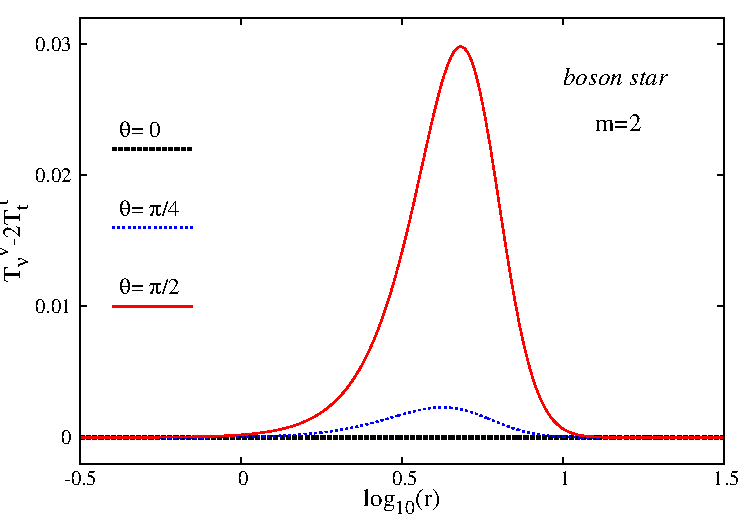
\includegraphics[width=8.1cm]{BS-ro-m2.pdf}
      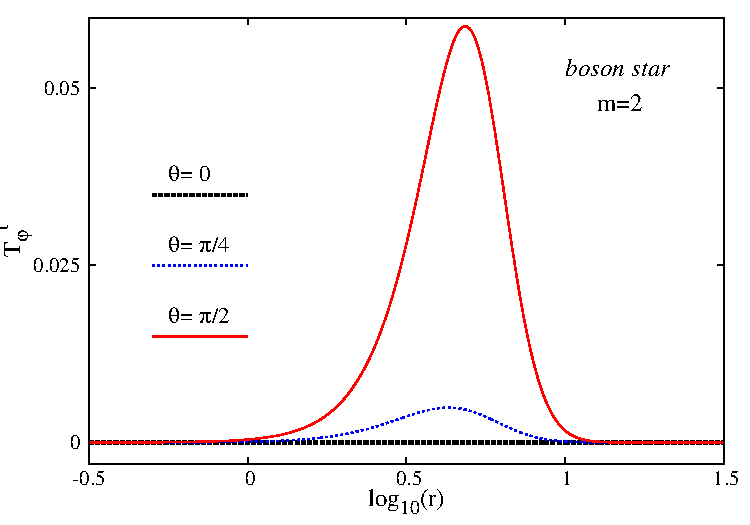
\includegraphics[width=8.1cm]{BS-T34-m2.pdf}
  \end{center}
 \caption{Same as in Fig.~\ref{PS1} but for $m=2$. Both solutions have $w=0.8$. The Proca star has $\mu M=2.319$, 
$\mu^2J=4.873$ whereas the scalar boson star has $\mu M=2.016$, $\mu^2J=4.272$.}
  \label{PS2}
\end{figure}


\begin{figure}[h!]
  \begin{center}
    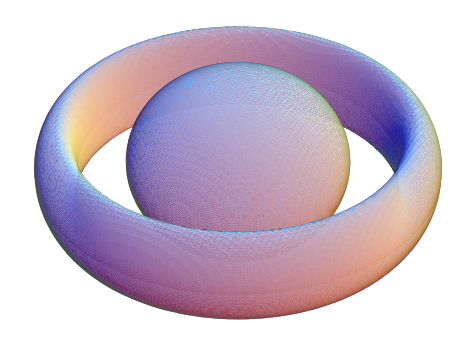
\includegraphics[width=6.1cm]{3DPS1-m=1-v2.pdf} \qquad \qquad 
       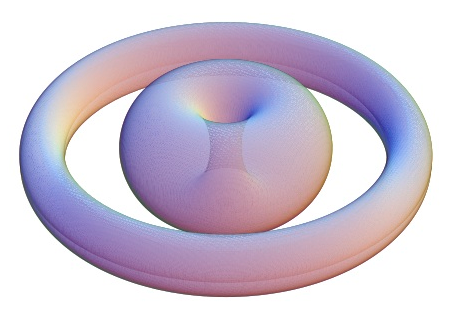
\includegraphics[width=6.1cm]{3DPS1-m=2-v2.pdf}   
         \end{center}
 \caption{Left (right) panel: Saturn-like (di-ring-like) surfaces of constant energy density for the $m=1$ ($m=2$) Proca star exhibited in Fig.~\ref{PS1} (Fig.~\ref{PS2}). The corresponding energy density is $0.011$ ($0.008$). We emphasize these are not embedding diagrams; rather we defined Cartesian coordinates regarding the $r,\theta,\varphi$ coordinate system used here as standard spherical coordinates.}
  \label{3D}
\end{figure}

Finally, we discuss how `compact' these Proca stars are. Proca stars, like their scalar cousins, have no surface, $i.e.$ the Proca field decays exponentially towards infinity. Thus, there is no unique definition of the Proca star's `radius'. To obtain an estimate we follow the discussion in~\cite{AmaroSeoane:2010qx,Herdeiro:2015gia}. Using the `perimeteral' radius, $i.e.$, a radial coordinate $R$ such that a circumference along the equatorial plane has perimeter $\simeq 2\pi R$,  we compute $R_{99}$, the perimeteral radius containing 99\% of the Proca star mass, $M_{99}$. Then, we define the inverse compactness by comparing $R_{99}$ with the Schwarzschild radius associated to 99\% of the Proca star's mass, $R_{Schw}=2M_{99}$:
%
\begin{equation}
{\rm Compactness}^{-1}\equiv  \frac{R_{99}}{2M_{99}} \ .
\label{compactness}
\end{equation}
%
The result for the inverse compactness of Proca stars with $m=1$ is exhibited in Figure~\ref{compactnessfig}. With this measure, the inverse compactness is always greater than unity; $i.e.$, Proca stars are less compact than BHs, as one would expect, but they are also less compact than comparable scalar boson stars.


\begin{figure}[h!]
  \begin{center}
    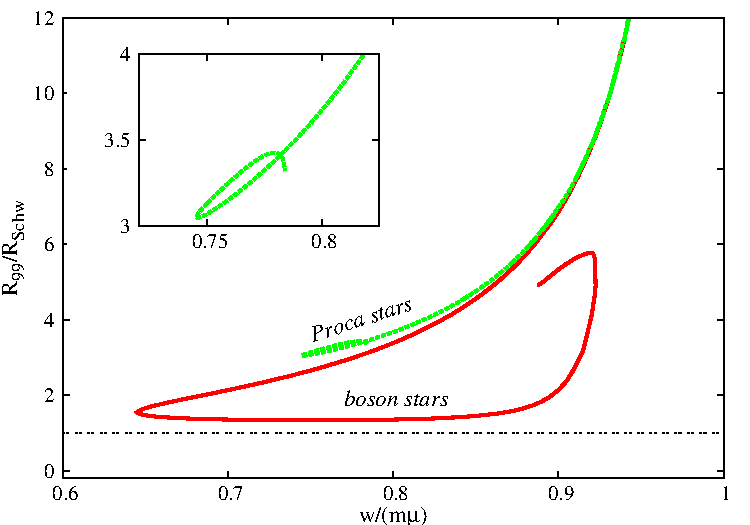
\includegraphics[width=8.1cm]{w-Comp-Schw.pdf}  
         \end{center}
 \caption{Inverse compactness of Proca stars compared to that of the scalar boson stars with $m=1$, defined in~\eqref{compactness}. The inset shows a detail of the Proca stars curve.}
  \label{compactnessfig}
\end{figure}




%%%%%%%%%%%%%%%%%%%%%%%%%%%%%%%%%%%%%%%%%%%%%%%%%%%%%%%%%%%%%%%%%%%%%%%%%%%%%%
\section{Kerr BHs with Proca Hair} 
\label{sec_kbhsph}
%%%%%%%%%%%%%%%%%%%%%%%%%%%%%%%%%%%%%%%%%%%%%%%%%%%%%%%%%%%%%%%%%%%%%%%%%%%%%%
We are now finally ready to tackle KBHsPH. The parallelism with the scalar case for both the stationary clouds and the solitonic limit is striking and one anticipates a high degree of similarity also at the level of the hairy BH solutions. 

The metric ansatz for constructing KBHsPH is the same as it was used for KBHsSH in~\cite{Herdeiro:2014goa}, and is precisely of the form~\eqref{kerrnc} with~\eqref{n}, where now 
all four (unspecified) functions $F_0,F_1,F_2,W$ depend on $(r,\theta)$ and, again, $r_H$ is a constant. If $F_2$ is finite, then $r={\rm constant}$ surfaces are timelike for $r>r_H$ and become null for $r=r_H$. Thus, $r=r_H$ is the location of the event horizon if the metric is regular therein.

For $r_H=0$, this ansatz reduces to the one discussed in the previous section for Proca stars, except for the replacement~\eqref{ww}. The line element form used for Proca stars is useful to tackle the behaviour at the origin, whereas the one used for BHs is useful to tackle the behaviour on a rotating horizon wherein $W$ reduces to the horizon angular velocity, $\Omega_H$. Indeed, following null geodesic generators ($ds^2=0$) on the horizon ($r=r_H$), assuming $F_2$ is finite therein, implies $d\varphi=W(r_H)dt$ and thus $W(r_H)=\Omega_H$, the angular velocity as measured by the observer at infinity.

The Proca field ansatz is the same as for the stationary Proca clouds (and Proca stars up to the replacement~\eqref{ww}),~\eqref{procaclouds}. This, again, introduces two parameters: $w>0$, $m\in \mathbb{Z}$. As for Proca stars we shall focus here on $m=1$, and take the sychronization condition~\eqref{synchronization} that we can rewrite in this context as (for general $m$)
\begin{equation}
\frac{w}{m}=W(r_H) =\Omega_H\ . 
\label{synchronization2}
\end{equation}
This condition was deduced in the context of a test field on the Kerr background and can be related to the threshold of superradiance. But it also has a different origin. In Appendix~\ref{appendixb}, we present the Einstein tensor and the Proca energy-momentum tensor associated to the ansatz discussed in this section. A careful inspection of the components of the energy-momentum tensor that have inverse powers of $N$,\footnote{A similar analysis can be made at the level of the components in an orthonormal frame, with similar conclusions.} and hence may diverge at the horizon, shows that, taking into account~\eqref{bccloudshorizon}, finiteness of the energy-momentum tensor components presented at $r=r_H$ \textit{requires}
\begin{equation}
\frac{w-mW(r_H)}{N(r_H)} 
\end{equation}
to be finite and hence it requires \eqref{synchronization2} (the same can be observed in the Einstein equations presented in~\cite{Herdeiro:2015gia}). It is interesting to remark that this finiteness condition~\eqref{synchronization2} is not necessarily related to superradiance, as the higher dimensional examples in~\cite{Brihaye:2014nba,Herdeiro:2015kha} illustrate. 




The Einstein-Proca equations are solved with the following boundary conditions (which again we have found to be compatible with an approximate construction of the solutions
on the boundary of the domain of integration):  
\begin{description}
\item[i)] at infinity, the same as for Proca stars,~\eqref{bccloudslarge} and~\eqref{bcstarslarge};
\item[ii)] on the symmetry axis, the same as for Proca stars,~\eqref{bccloudsaxis} and~\eqref{bcstarsaxis};
 
\item[iii)] at the horizon, using again the new radial coordinate $x=\sqrt{r^2-r_H^2}$, a power series expansion near $x=0$ implies~\eqref{bccloudshorizon}, together with
\begin{equation}
\partial_x F_i\big|_{x=0}=0 \ , \qquad W\big|_{x=0}=\Omega_H \ .
\end{equation}
\end{description}
 % 
 
The Einstein-Proca equations for KBHsPH are quite involved (Appendix B). They are solved numerically, subject to the above boundary conditions, by  using the elliptic PDE solver \textsc{fidisol/cadsol}~\cite{schoen} 
based on a finite differences method in conjunction with the Newton-Raphson procedure. 
A description of the method for the case of KBHsSH can be found in~\cite{Herdeiro:2015gia}. 
The procedure in the case at hand is analogous. 

 


%%%%%%%%%%%%%%%%%%%%%%%%%%%%%%%%%%%%%%%%%%%%%%%%%%%%%%%%%%%%%%%%%%%%%%%%%%%%%%%
\subsection{Physical Quantities}
\label{subsec_II}
%%%%%%%%%%%%%%%%%%%%%%%%%%%%%%%%%%%%%%%%%%%%%%%%%%%%%%%%%%%%%%%%%%%%%%%%%%%%%%% 
In the following we shall describe some physical quantities that will be monitored from the numerical solutions we have obtained.  The ADM mass, $M$, and ADM angular momentum, $J$, are read off from the asymptotic expansion of the appropriate metric components:
%
\begin{equation}
\label{asym}
g_{tt} =-1+\frac{2M}{r}+\dots \ ,\qquad ~~g_{\varphi t}=-\frac{2J}{r}\sin^2\theta+\dots \ . \ \ \ 
\end{equation}
%
We also compute the horizon mass and angular momentum by using the appropriate Komar integrals associated to the corresponding Killing vector fields ${\bf k}$ and ${\bf m}$:
\begin{equation}
M_H=-\frac{1}{8\pi}\oint_{\mathcal{H}}dS_{\alpha\beta}D^\alpha k^\beta \ , \qquad 
J_H=\frac{1}{16\pi}\oint_{\mathcal{H}}dS_{\alpha\beta}D^\alpha m^\beta \ .
\end{equation}
%
%
Of course, $M$ and $J$ can also be computed as Komar integrals at infinity. Then, applying Gauss's law, one obtains a relation with $M_H$ and $J_H$ together with volume integrals on a spacelike surface with a boundary at the (spatial section of the) horizon. By making use of the Killing identity and the Einstein equations one obtains:
\begin{equation}
M=M_H-2\int_{\Sigma}dS_{\alpha}\left(T^\alpha_\beta k^\beta-\frac{1}{2}Tk^\alpha\right) \equiv M_H+M^{(\mathcal{P})}
\end{equation}
This defines the energy stored in the Proca field (outside the horizon):
\begin{equation}
M^{({\cal P})}\equiv - \int_{\Sigma} dr d\theta d\varphi(2T_t^t-T_\alpha^\alpha) \sqrt{-g} \ .
\label{ed}
\end{equation}
%
Proceeding similarly for the angular momentum one obtains:
\begin{equation}
J=J_H+J^{(\mathcal{P})} \ , \ \qquad  J^{({\cal P})}\equiv  \int_{\Sigma} dr d\theta d\varphi T^t_\varphi \sqrt{-g} \ ,
\label{amd}
\end{equation}
which defines the angular momentum stored in the Proca field. At this point, an interesting distinction arises, with respect to the scalar case. 
 Whereas for KBHsSH the angular momentum stored in the scalar field relates to the Noether charge in precisely the same way as for rotating scalar boson stars $J^{(\Psi)}=mQ$, for KBHsPH the relation between $J^{(\mathcal{P})} $ and  the Noether charge~\eqref{q} includes an extra boundary term (see Appendix~\ref{appendixc} and eq.~\eqref{JQBHs})
\begin{equation}
\label{nr1}
J^{(\mathcal{P})}=mQ+ \oint_\mathcal{H}  ({\mathcal{A}}_\varphi \bar{ {\mathcal{F}}}^{r t}+\bar{\mathcal{A}}_\varphi { {\mathcal{F}}}^{r t}  ) dS_r \ ,
\end{equation}
which generalizes relation~\eqref{amnc} to the case of hairy BHs. 
A similar relation can be written for $M^{({\cal P})}$ (see Appendix \ref{appendixc}
and eq. (\ref{sup1}))
\begin{equation}
\label{nr2}
M^{({\cal P})}=2w Q
-\mu^2  {\cal U}
+ \oint_\mathcal{H}  
\left[
\frac{1}{2} 
\left(
{\mathcal{A}}_\beta \bar{ {\mathcal{F}}}^{r \beta}+\bar{\mathcal{A}}_\beta { {\mathcal{F}}}^{r \beta}
\right)
-\left({\mathcal{A}}_t \bar{ {\mathcal{F}}}^{r t}+\bar{\mathcal{A}}_t { {\mathcal{F}}}^{r t}
\right)  
\right] dS_r \ ,
\end{equation}
with
\begin{equation}
\label{U}
{\cal U}\equiv \int _\Sigma  dr d\theta d\varphi  {\mathcal{A}}_\alpha \bar {\mathcal{A}}^\alpha \sqrt{-g}\ .
\end{equation}


The horizon temperature and event horizon area of the KBHsPH solutions are computed by standard relations, that specialize to: 
\begin{eqnarray}
\label{THAH}
T_H=\frac{1}{4\pi r_H}e^{(F_0-F_1)|_{r=r_H}} \ , \qquad
 A_H=2\pi r_H^2 \int_0^\pi d\theta \sin \theta  e^{(F_1+F_2)|_{r=r_H}}\ . 
 \end{eqnarray}
Then, the ADM quantities $M,J$ are related with $T_H,S,Q,M^{({\cal P})}$, where $S=A_H/4$ is the horizon entropy, through a Smarr formula  
%
\begin{eqnarray}
\label{smarr} 
M=2 T_H S +2\Omega_H J_H+ M^{({\cal P})} \ .
% \nonumber
%\\
%- \int_{\Sigma} dr d\theta d\varphi(2T_t^t-T_a^a) \sqrt{-g},
\end{eqnarray}
Also, the variation of $M$ can be expressed by the first law:
\begin{equation}
\label{fl}
dM=T_H dS +\Omega_H dJ \ .
%= T_H dS +\Omega_HdJ_H+wdQ \ .
\end{equation}
We note that
by making use of the relations
(\ref{nr1})
and
(\ref{nr2}),
 the Smarr formula (\ref{smarr})
can be written in a Kerr-like form
\begin{eqnarray}
\label{smarr-new1} 
M=2 T_H S +2\Omega_H J-\mu^2 {\cal U} \ ,
\end{eqnarray}
which renders explicit the fact that the solutions are supported by
a nonzero mass term of the Proca field.

Finally, we observe that Proca stars
satisfy a simple relation, which results again from 
(\ref{nr1}),
(\ref{nr2}):\footnote{One can similarly show that KBHsSH and scalar boson stars satisfy relations analogous to
(\ref{smarr-new1}) and  (\ref{smarr-new2}), respectively.} 
\begin{eqnarray}
\label{smarr-new2} 
M=2 w Q-\mu^2 {\cal U}=2\frac{w}{m} J-\mu^2 {\cal U}\ .
\end{eqnarray}



%%%%%%%%%%%%%%%%%%%%%%%%%%%%%%%%%%%%%%%%%%%%%%%%%%%%%%%%%%%%%%%%%%%%%%%%%%%%%%%
\subsection{The domain of existence and phase space}
\label{subsec_III}
%%%%%%%%%%%%%%%%%%%%%%%%%%%%%%%%%%%%%%%%%%%%%%%%%%%%%%%%%%%%%%%%%%%%%%%%%%%%%%% 
We have scanned the domain of existence of KBHsPH by varying $r_H$ for fixed $w$ lines (or vice-versa), 
in between the minimum frequency 
$w_{\rm min}/\mu=0.7453$ and the maximal one $w=\mu$. 
The result for the $m=1$ family of KBHsPH is shown in Fig.~\ref{figdomain} (left panel), 
together with the analogous family of KBHsSH (right panel), the former obtained from over five thousand numerical points. 


%
\begin{figure}[h!]
  \begin{center}
    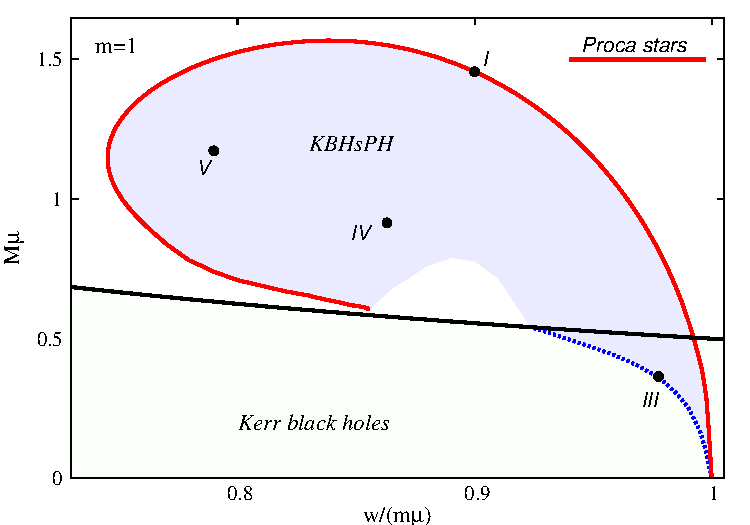
\includegraphics[width=8.1cm]{BH-w-M-with-points.pdf}
      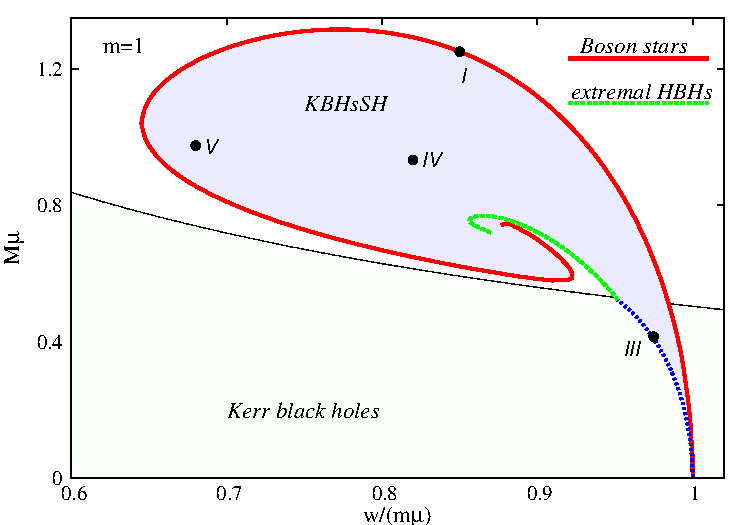
\includegraphics[width=8.1cm]{scalar-BH-w-M.pdf}
  \end{center}
  \caption{ADM mass $vs.$ frequency $w$ diagram for $m=1$ KBHsPH (left panel) and KBHsSH (right panel). The red solid lines correspond to the solitonic limit (Proca stars and scalar boson stars, respectively, already shown in Fig.~\ref{clouds}). The blue dotted lines are the Kerr limit, also shown in Fig.~\ref{clouds}. Kerr solutions exist below the black solid line, which corresponds to extremal Kerr solutions. The hairy BHs exist in the blue shaded region. Points I,III,IV,V, in each case, correspond to specific solutions for which the numerical data is publicly available~\cite{datakbhph,datakbhsh}. The right panel also shows the extremal hairy BHs (green dashed) line.}
  \label{figdomain}
\end{figure}
%


Based on the discussions of KBHsSH~\cite{Herdeiro:2014goa,Herdeiro:2015gia,Herdeiro:2015tia}, and as already partly discussed, the domain of existence of KBHsPH should be bounded by three lines: the Proca clouds existence line discussed in Section~\ref{sec_clouds}, the Proca star line discussed in Section~\ref{sec_stars} and the line of extremal KBHsPH ($i.e.$ zero temperature). So far, the last of the three were only obtained by extrapolating to $T_H=0$ the non-extremal solutions, as our attempts to construct the extremal KBHsPH solutions by directly solving the Einstein-Proca field equations were unsuccessful (unlike the scalar case, as reported in~\cite{Herdeiro:2015gia}). For this reason we have chosen not to display this line in Fig.~\ref{figdomain}, for the Proca case.  Another technical difficulty arises in trying to connect the set of (extrapolated) extremal solutions with the set of Proca stars. As for the case of KBHsSH, these two curves are likely to meet in a critical point at the center of the 
Proca stars spiral; however, validation of this hypothesis is a numerical challenge (also for KBHsSH).

Concerning numerical errors, the PDE solver we have used provides error estimates for each unknown function, which allows judging the quality of the computed solution. The numerical error for the solutions reported in
this work is estimated to be typically $<10^{-3}$. As a further check of the numerical procedure, we have verified that the families of solutions  satisfy with a very good accuracy the first law of thermodynamics and also the Smarr relation, typically at that same order. We have also monitored the violation of the gauge condition together with the constraint Einstein equations; typically, these provide much lower estimates for the numerical errors. As a comparative comment, the overall quality of the solutions is, however,  not as high for KBHsPH as for KBHsSH.
Additionally, the source of the difficulties we have encountered in constructing extremal and close to extremal solutions are absent in the scalar case. Typically, for the Proca case, the solver stops to converge in the near extremal case,
 although the error estimates for the last solutions is still small. It is likely that another metric parametrization is required to tackle this issue. We also remark that  there may be a more involved landscape of excited solutions in view of the four vector potentials.\footnote{ 
In fact, we have observed that the solver frequently ``jumps"  to one of these excited configurations 
which is not too far in the parameter space.}

In Fig.~\ref{figdomain} we have singled out four particular solutions for each case, denoted I,III,IV and V. The numerical data for these four solutions, together with the data for a vacuum Kerr solution with the same ADM mass and angular momentum as that of configuration III, for each case, has been made publicly available for community use~\cite{datakbhph,datakbhsh}. The corresponding parameters are detailed in Appendix~\ref{appendixd}.

In Fig.~\ref{fig2} we exhibit the phase space, $i.e.$ ADM mass $vs.$ ADM angular momentum diagram for $m=1$ solutions of KBHsPH (left panel) and as a comparison, the corresponding diagram for KBHsSH (right panel). The two plots are quite similar and the features we wish to emphasize is that, as for the scalar case, one observes violation of the Kerr bound (in terms of ADM quantities) and non-uniqueness, $i.e$ there are both hairy and vacuum Kerr BHs with the same ADM mass and angular momentum ($cf.$ Appendix~\ref{appendixd}). 


%\begin{widetext}
%
\begin{figure}[h!]
  \begin{center}
    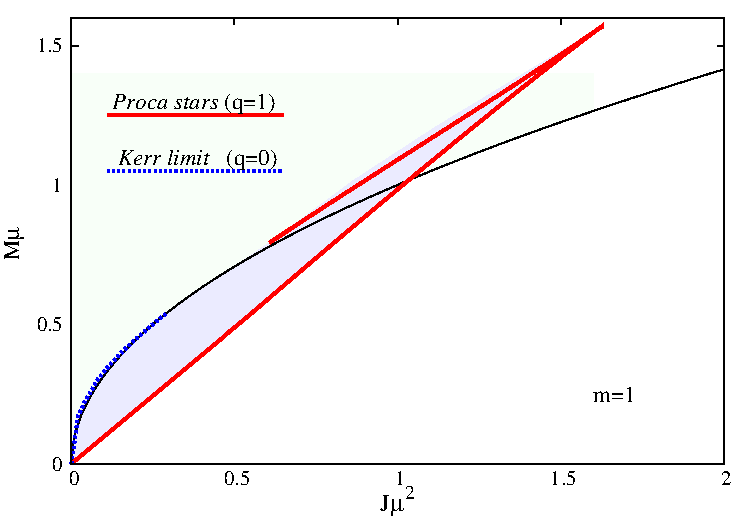
\includegraphics[width=8.1cm]{BH-J-M.pdf}
      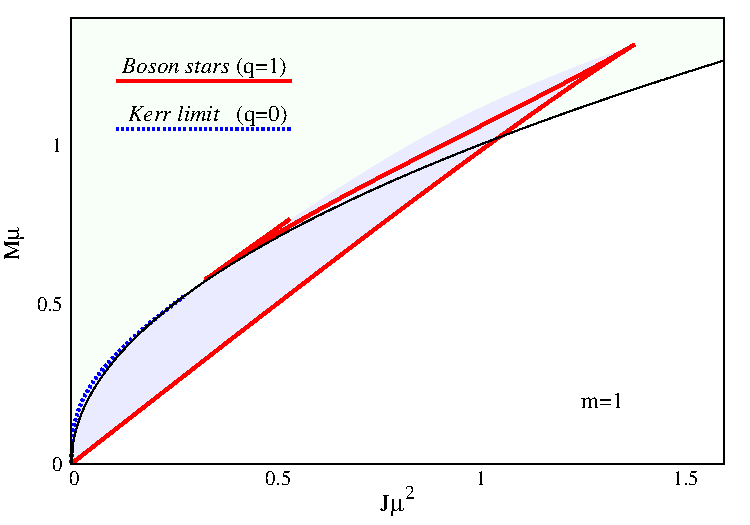
\includegraphics[width=8.1cm]{scalar-BH-J-M.pdf}
  \end{center}
  \caption{ADM mass $vs.$ ADM angular momentum diagram for $m=1$ KBHsPH (left panel) and KBHsSH (right panel), in units of the field mass. The black solid line corresponds to extremal Kerr solutions; non extremal BHs exist above this line. The red solid line is for Proca (scalar boson) stars in the left (right) panel. The blued dotted line is the existence line, denoting Kerr BHs that support Proca (scalar) clouds. The blue shaded region is the domain of existence of KBHsPH (KBHsSH).}
  \label{fig2}
\end{figure}
 

The violation of the Kerr bound also occurs in terms of \textit{horizon} quantities, as shown in Fig.~\ref{vconjecture} (right panel). For these solutions the conjecture put forward in~\cite{Herdeiro:2015moa} concerning the horizon linear velocity $v_H$, as defined therein, holds: despite violating the Kerr bound both in terms of ADM and horizon quantities, $v_H$ never exceeds the speed of light.  We recall $v_H$ is defined as follows, for asymptotically flat, stationary and axi-symmetric spacetimes. On a spatial section of the event horizon one computes the proper length of all closed orbits of ${\bf m}$. Let $L_{\rm max}$ be the maximum of all such proper lengths; the corresponding circumferencial radius, $R_c$, is $R_c\equiv {L_{\rm max}}/({2\pi})$. 
The horizon linear velocity is $v_H \equiv R_c \Omega_H$ \cite{Herdeiro:2015moa}.
 





\begin{figure}[h!]
  \begin{center}
    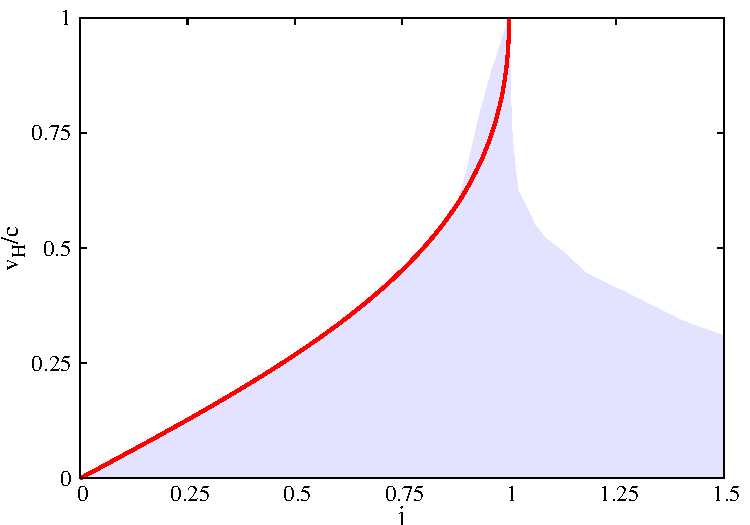
\includegraphics[width=8.1cm]{ProcaBH-j-v-bound.pdf}
      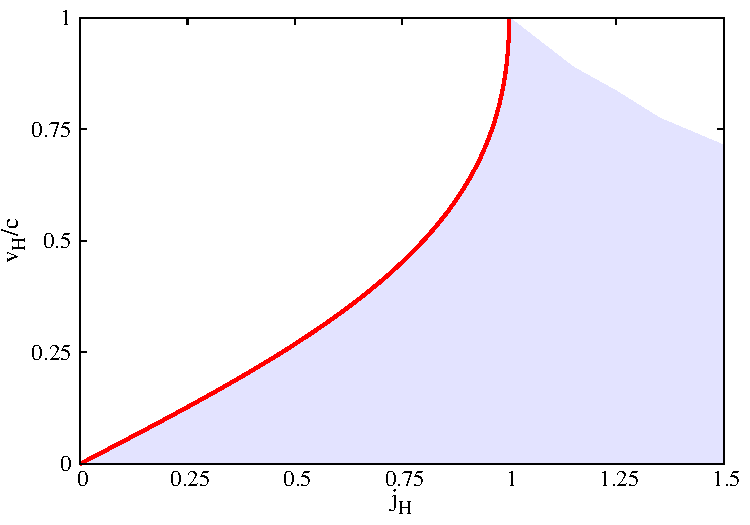
\includegraphics[width=8.1cm]{ProcaBH-jKv-bound.pdf}
  \end{center}
 \caption{Linear velocity of the horizon normalized to the speed of light, $v_H$, versus:  (left panel)  the ADM dimensionless spin parameter $j\equiv Jc/GM^2$, where $M,J$ are the ADM mass and angular momentum; (right panel) the horizon dimensionless spin parameter $j_H\equiv J_Hc/GM_H^2$, where $M_H,J_H$ are the horizon mass and angular momentum. Here we have reinstated $c,G$. The red solid line corresponds to vacuum Kerr and the shaded area is filled by KBHsPH.}
  \label{vconjecture}
\end{figure}







%%%%%%%%%%%%%%%%%%%%%%%%%%%%%%%%%%%%%%%%%%%%%%%%%%%%%%%%%%%%%%%%%%%%%%%%%%%%%%%
\subsection{Energy distribution and horizon quantities}
\label{subsec_IV}
%%%%%%%%%%%%%%%%%%%%%%%%%%%%%%%%%%%%%%%%%%%%%%%%%%%%%%%%%%%%%%%%%%%%%%%%%%%%%%%
As for their scalar cousins, KBHsPH can be thought of as a bound state of a horizon with a Proca star. Thus, the matter energy density distribution around the horizon will resemble that of (some) Proca stars. In~Fig.~\ref{figenergybhs}  we exhibit the energy density and the angular momentum density as a function of the radial coordinate for different angular sections for an example of KBHPH. As for the Proca stars, both the energy density and the angular momentum density can have more than one maximum outside the horizon and the latter can also have regions with a different sign. Thus, outside KBHsPH there are counter-rotating regions. In Fig.~\ref{fig3Dbh} a constant Proca energy density surface is exhbited in a 3D plot. The behaviour of the energy density and angular momentum density on the horizon is more clearly seen in Fig.~\ref{horizoned}.


\begin{figure}[h!]
  \begin{center}
    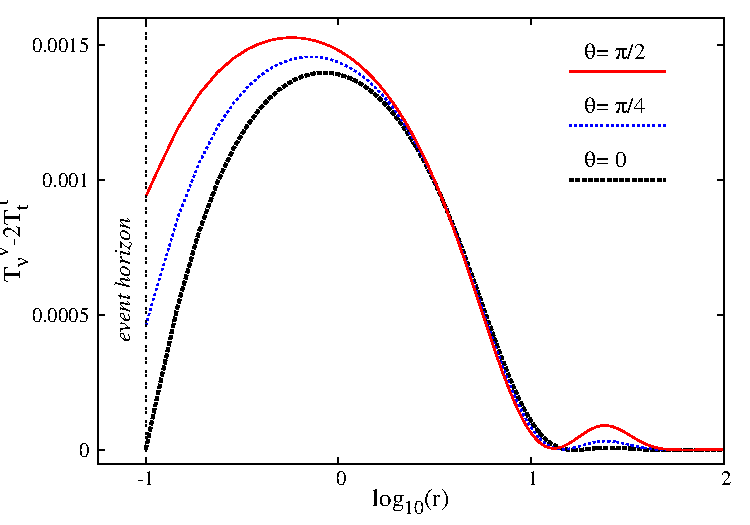
\includegraphics[width=8.1cm]{BH-ro-m1.pdf}
      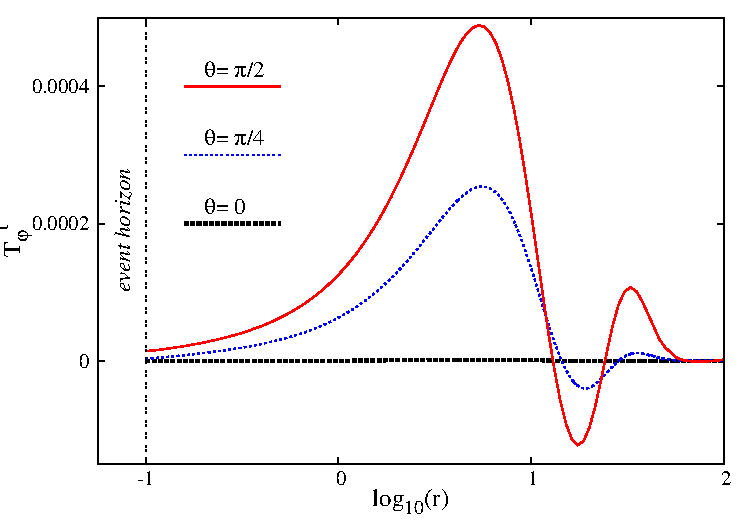
\includegraphics[width=8.1cm]{BH-T34.pdf}
  \end{center}
  \caption{Radial variation of the energy density, $cf.$~\eqref{ed} (left panel), and angular momentum density, $cf.$~\eqref{amd}  (right panel),  of the Proca field, for different constant $\theta$ sections of a KBHPH with $m=1$, $w=0.98\mu$, $r_H=0.1$,  $\mu M=0.701$ and $\mu^2J=0.652$.}
  \label{figenergybhs}
\end{figure}



\begin{figure}[h!]
  \begin{center}
    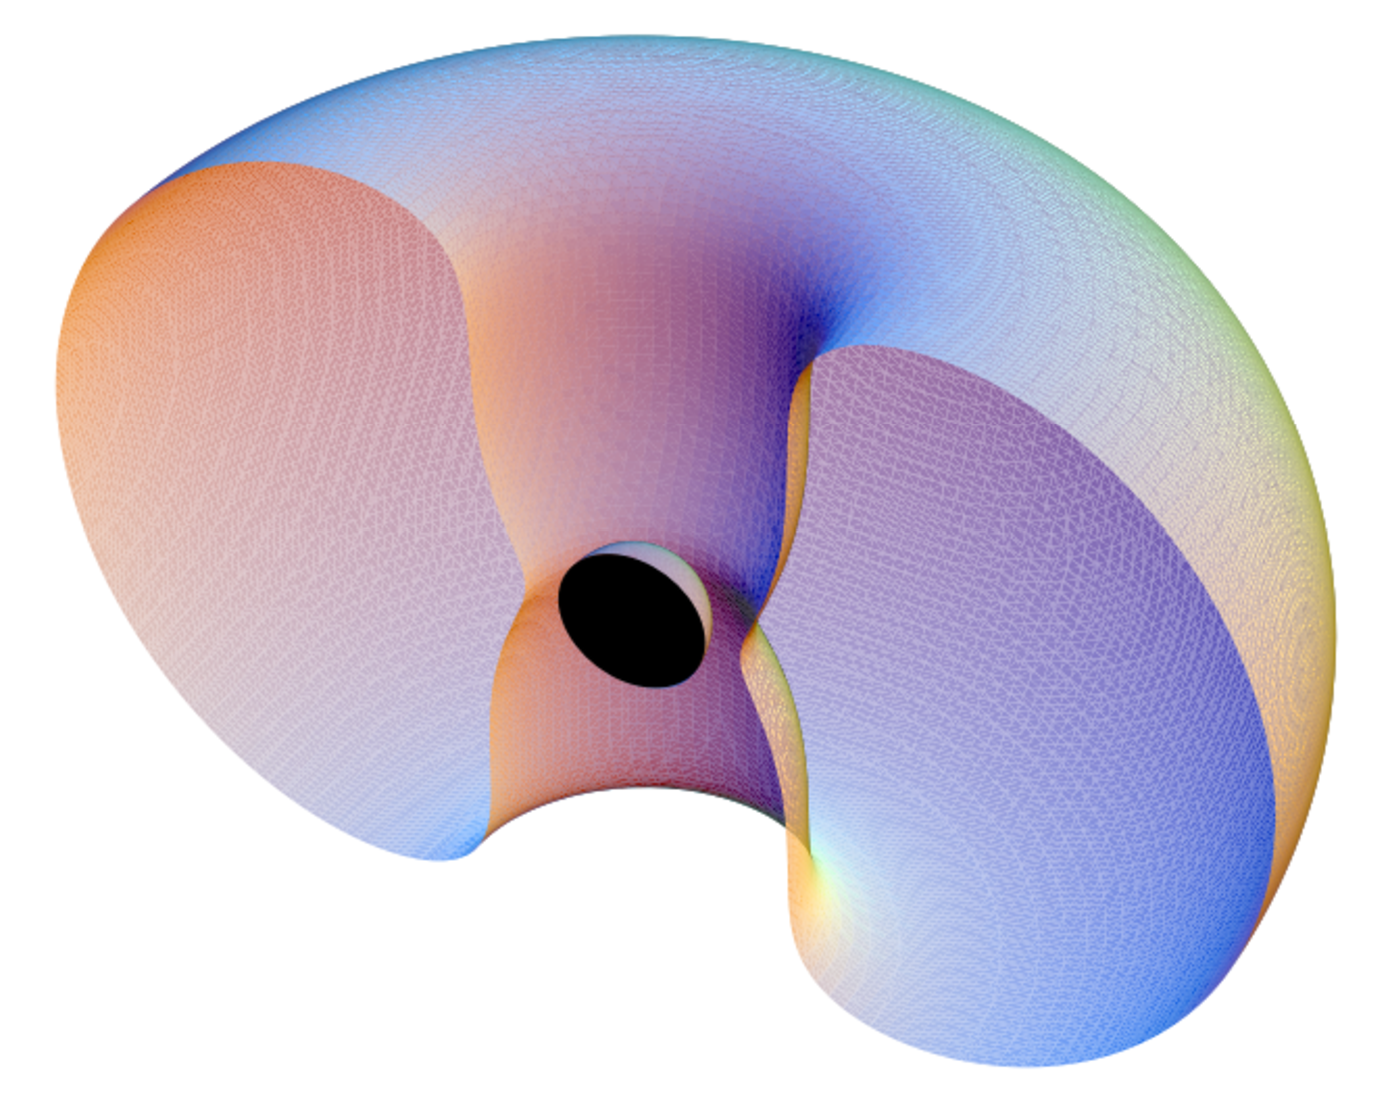
\includegraphics[width=6.1cm]{3Dbh.pdf}
  \end{center}
  \caption{One toroidal-like surface of constant energy density (corresponding to $0.00142$) for the same KBHPH displayed in Fig.~\ref{figenergybhs}. We also plot the spatial section of the event horizon in these coordinates (half-sphere with the black cross section).}
  \label{fig3Dbh}
\end{figure}


\begin{figure}[h!]
  \begin{center}
    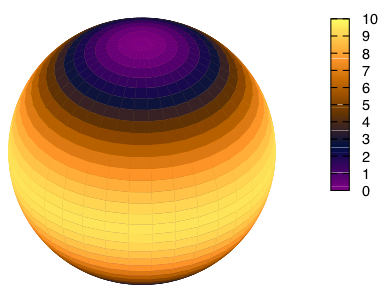
\includegraphics[width=5.5cm]{Ttr-horizon.pdf}\qquad \qquad 
      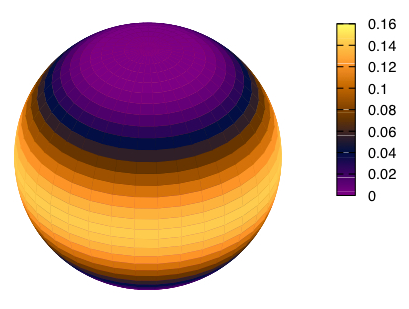
\includegraphics[width=6.0cm]{T34-horizon.pdf}
  \end{center}
  \caption{Energy density, $cf.$~\eqref{ed} (left panel), and angular momentum density, $cf.$~\eqref{amd}  (right panel),  of the Proca field on the horizon for the same example of a KBHPH displayed in Fig.~\ref{figenergybhs}. The corresponding values were multiplied by $10^4$ for better visualization.}
  \label{horizoned}
\end{figure}


Finally, in Fig.~\ref{temperature} we exhibit the variation of the horizon area with the horizon temperature along sequences of solutions with constant horizon angular velocity (or frequency). For both KBHsPH (left panel) and KBHsSH (right panel) one can see three different types of behaviour, which are easy to interpret referring back to Fig.~\ref{figdomain}. For large values of $\Omega_H$, the solutions interpolate between the Kerr existence line and the corresponding (Proca or scalar boson) star line (for which $T_H\rightarrow \infty$). For intermediate values of $\Omega_H$, the solutions interpolate between the extremal BHs line (for which $T_H\rightarrow 0$) and the corresponding star line. Finally, for sufficiently small values of $\Omega_H$, the solutions interpolate between two stars, and thus start and end for $T_H\rightarrow \infty$.


\begin{figure}[h!]
  \begin{center}
    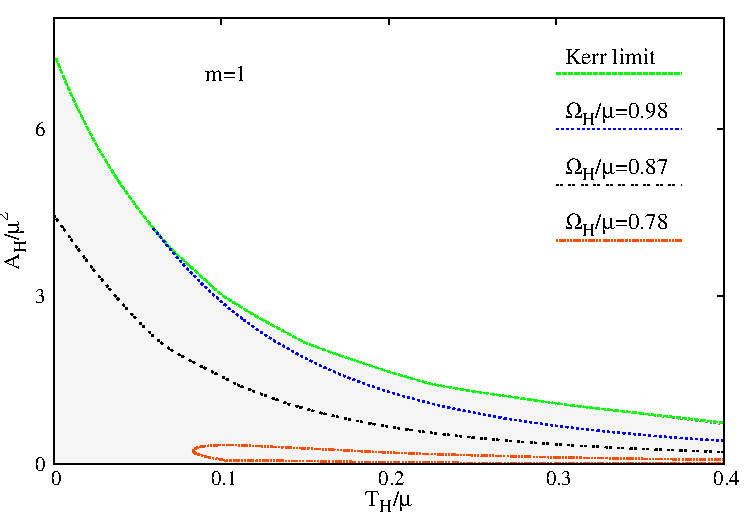
\includegraphics[width=8.1cm]{BH-TH-AH.pdf}
      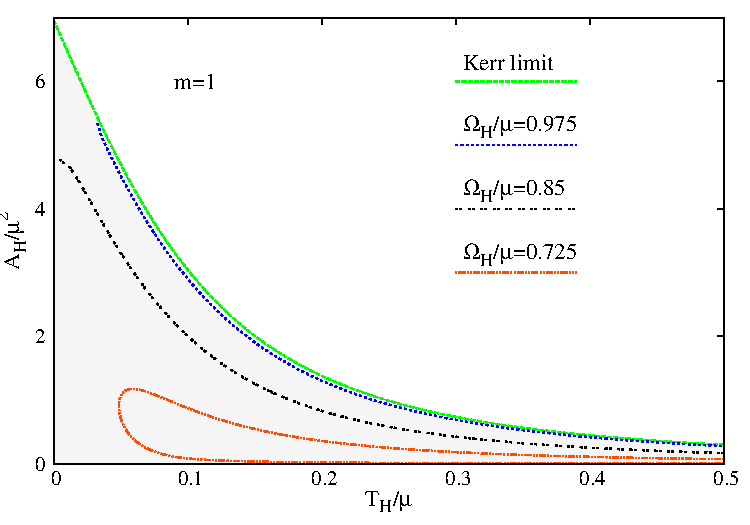
\includegraphics[width=8.1cm]{scalar-BH-TH-AH.pdf}
  \end{center}
 \caption{Event horizon area $vs.$ temperature for KBHsPH (left panel) and KBHsSH (right panel), in units of $\mu$, for different constant angular velocity sets of solutions.}
  \label{temperature}
\end{figure}






%%%%%%%%%%%%%%%%%%%%%%%%%%%%%%%%%%%%%%%%%%%%%%%%%%%%%%%%%%%%%%%%%%%%%%%%%
\section{Discussion}
\label{sec_discussion}
%%%%%%%%%%%%%%%%%%%%%%%%%%%%%%%%%%%%%%%%%%%%%%%%%%%%%%%%%%%%%%%%%%%%%%%%%%%%%%%
It has long been established that stationary, asymptotically flat BHs in Einstein's gravity minimally coupled to one or many real, Abelian Proca fields cannot have Proca hair. The basic theorem supporting this idea, due to Bekenstein~\cite{Bekenstein:1971hc,Bekenstein:1972ky}, assumes, however, that the Proca field inherits the spacetime isometries. In this paper we have shown that dropping this assumption Kerr BHs with Proca hair exist under two conditions:
\begin{description}
\item[i)] The Proca field is complex, or equivalently there are two real Proca fields with the same mass. Solutions in this paper can be, moreover, generalized to an arbitrary number of complex Proca fields (any even number of real Proca fields), without mutual interactions, and all of them minimally coupled to gravity. Here, however, we focus on a model with a single complex Proca field. 
\item[ii)] The complex Proca field has a harmonic time dependence, as in the ansatz~\eqref{procaclouds}, with the frequency and azimuthal harmonic index obeying the synchronization condition~\eqref{synchronization}.
\end{description}
These two assumptions, together, allow the two real Proca fields to oscillate, with the same frequency but opposite phases, hence cancelling out gravitational radiation emission (as well as Proca radiation emission). It remains as an open question if the same could be achieved with a single real Proca field, especially in view of the result in~\cite{Wang:2015fgp}, since such real Proca field already has two independent modes. 

\bigskip

The existence of  KBHsPH -- to the best of our knowledge the first example of (fully non-linear)   
BHs with (Abelian) vector hair -- is anchored  in the synchronization/superradiance zero mode condition
($i.e.$ the field should co-rotate with the  black hole horizon). 
%
All previously constructed examples which employed this mechanism have scalar hair, 
both in four spacetime dimensions~\cite{Herdeiro:2014goa,Herdeiro:2015gia,Kleihaus:2015iea,Herdeiro:2015tia} and in higher dimensions~\cite{Brihaye:2014nba,Herdeiro:2015kha}, 
including the example in five dimensional asymptotically Anti-de-Sitter space found in~\cite{Dias:2011at}. 
This further shows the generality of the mechanism and lends support to the conjecture in~\cite{Herdeiro:2014goa,Herdeiro:2014ima}.

We also remark that  the Proca model considered here can be regarded as a proxy 
for more realistic models with a gauged scalar field, where the gauge fields acquire a mass \textit{dynamically}, via the Higgs mechanism. A familiar example in this direction is the non-Abelian Proca model,
whose solutions contain already all basic properties of the Yang-Mills--Higgs sphalerons
% which arise dynamically from  Yang-Mills---Higgs solutions 
in the Standard Model \cite{Greene:1992fw}. 
%
As such, the results in this work suggest that one should
reconsider the no-hair theorem for the Abelian-Higgs model~\cite{Adler:1978dp}.


\bigskip

Several direct generalizations/applications of these solutions are possible. 
At the level of constructing further 
solutions, we anticipate that 
$(i)$ self-interacting Proca hair will lead to new solutions, 
which, if the scalar field case is a good guide~\cite{Herdeiro:2015tia}, can have a much larger ADM mass (but not horizon mass)
and
$(ii)$ hybrid solutions with scalar plus Proca hair are possible. 
At the level of possible astrophysics phenomenology, 
it would be interesting to look in detail to the geodesic flow, 
in particular to the frequency at the innermost stable circular orbit (ISCO), 
quadrupoles as well as to the lensing and shadows of these new BHs,
following~\cite{Cunha:2015yba} (see also the review~\cite{Johannsen:2015mdd}). 
Work in this direction is underway.

\bigskip

 Finally, it is still a common place to find in the current literature statements that stationary BHs in GR are described solely by mass, angular momentum and charge. We want to emphasize that the examples of Kerr BHs with scalar and Proca hair show that this is \textit{not true as a generic statement for GR, even if physical matter -- i.e. obeying all energy conditions -- is required.} These examples show that Noether charges, rather than charges associated to Gauss laws, are also permitted in non-pathological stationary, asymptotically flat, BH solutions. The main outstanding questions is if in a real dynamical process these Noether charges can survive.
 
 

\vspace{0.5cm} 
 %%%%%%%%%%%%%%%%%%%%%%%%%%%%%%%%%%%%%%%%%%%%%%%%%%%%%%%%%%%%%%%%%%%
\noindent
\section*{Acknowledgements}
We would like to thank Richard Brito and Vitor Cardoso for a fruitful collaboration on Proca stars. We also thank J. Rosa, M. Sampaio and M. Wang for discussions on Proca fields. C. H. and E. R. acknowledge funding from the FCT-IF programme. H.R. is supported by the grant PD/BD/109532/2015 under the MAP-Fis Ph.D. programme. This work was partially supported by  the  H2020-MSCA-RISE-2015 Grant No.  StronGrHEP-690904, and by the CIDMA project UID/MAT/04106/2013. Computations were performed at the Blafis cluster, in Aveiro University.
 
 \bigskip
 
\appendix

%\newpage
%%%%%%%%%%%%%%%%%%%%%%%%%%%%%%%%%%%%%%%%%%%%%%%%%%%%%%%%%%%%%%%%%%%%%%%%
\section{Spheroidal prolate coordinates for Kerr}
\label{prolatecoordinates}
%%%%%%%%%%%%%%%%%%%%%%%%%%%%%%%%%%%%%%%%%%%%%%%%%%%%%%%%%%%%%%%%%%%%%%%%
The new coordinate system for Kerr~\eqref{kerrnc}, with the functions~\eqref{functionsKerr}, first introduced in~\cite{Herdeiro:2015gia}, actually reduce to spheroidal \textit{prolate} coordinates in the Minkowski space limit, but with a non-standard radial coordinate. To see this, we observe that, from~\eqref{Kerr2}, $M=0$ occurs when $r_H=-2b$. Then, from the expressions~\eqref{functionsKerr}, the metric~\eqref{kerrnc} becomes
\begin{eqnarray}
ds^2=-dt^2+\left[N(r)+\frac{b^2}{r^2}\sin^2\theta\right]\left[\frac{dr^2}{N(r)}+r^2d\theta^2\right]
+N(r)r^2\sin^2\theta d\varphi^2 \ , \qquad N(r)\equiv 1+\frac{2b}{r} \ .
\end{eqnarray}
This can be converted to the standard Minkowski Cartesian quadratic form $ds^2=-dt^2+dx^2+dy^2+dz^2$ by the spatial coordinate transformation
\begin{equation}
\left\{
\begin{array}{l}
x=r\sqrt{N(r)}\sin\theta\cos\varphi \ , \\
y=r\sqrt{N(r)}\sin\theta\sin\varphi \ , \\
z=(r+b)\cos\theta \ .
\end{array}
\right.
\end{equation}
A surface with $r=$constant is, in Cartesian coordinates,
\begin{equation}
\frac{x^2+y^2}{\bar{r}^2}+\frac{z^2}{\bar{r}^2+b^2}=1 \ ,
\end{equation}
where $\bar{r}=r\sqrt{N(r)}$. This is a prolate spheroid. It is interesting that KBHsSH and KBHsPH seem to prefer prolate spheroidal coordinates rather than the oblate spheroidal coordinates so well adapted to Kerr (in the Boyer-Lindquist form).





\section{Einstein-Proca equations of motion}
\label{appendixb}



Here we provide explicit expressions for the equations of motion solved by KBHsPH. The components of the Einstein tensor for the ansatz~\eqref{kerrnc} are:



\begin{eqnarray}
&&  4r^2  e^{2F_1}{\bf G_{tt}}= 4 
N \left[r^2 ({F_1}_{,rr}+ {F_2}_{,r}^2+
{F_2}_{,rr})
+r( 
{F_1}_{,r}+3  {F_2}_{,r})+1\right] + 2 r N'  \left(r 
{F_1}_{,r}+r {F_2}_{,r}+2\right)+4 {F_1}_{,\theta\theta}\nonumber \\
%
&& +4  
{F_2}_{,\theta}^2+4  {F_2}_{,\theta\theta}
%
+8
\cot \theta {F_2}_{,\theta}-4 
%
 +r^4 \sin ^2\theta e^{2 ({F_2}-F_0)} 
 \left\{
 \frac{2W W_{,r}}{r}(- r {F_0}_{,r} +3r{F_2}_{,r}+4 )
 +W_{,r}^2+2W W_{,rr} 
 \right. \nonumber \\ 
%
&& \left. + \frac{2 W \left[W_{,\theta} \left(- 
{F_0}_{,\theta}+3 {F_2}_{,\theta}+3 \cot\theta\right)+ W_{,\theta\theta}\right]+ W_{,\theta}^2}{r^2N} \right\},
\end{eqnarray}

\begin{equation}
\frac{2Ne^{2(F_0+F_1-F_2)}}{\sin^2\theta}{\bf G_{t\phi }}=   W_{,\theta} \left[ {F_0}_{,\theta}-3 \left( 
{F_2}_{,\theta}+\cot\theta\right)\right]- \left\{r N 
\left[W_{,r} \left(-r {F_0}_{,r}+3 r 
{F_2}_{,r}+4\right)+r 
W_{,rr}\right]+W_{,\theta\theta}\right\}  ,
\end{equation}



\begin{eqnarray}
&&  \frac{e^{2F_1}}{N}{\bf G_{rr}}= \frac{({F_0}_{,\theta}+\cot\theta)({F_0}_{,\theta}-{F_1}_{,\theta}+
{F_2}_{,\theta})+{F_2}_{,\theta}({F_2}_{,\theta}-{F_1}_{,\theta})
+{F_0}_{,\theta\theta}+{F_2}_{,\theta\theta}-1+[Nr]'}{r^2 N}+{F_1}_{,r} {F_2}_{,r}\nonumber \\
&& 
%2{F_0}_{,r} +{F_1}_{,r}+{F_2}_{,r}
%
+\frac{2{F_0}_{,r}+{F_1}_{,r}+{F_2}_{,r}}{r}(1+r)+\frac{e^{2(
{F_2}- {F_0})} \sin ^2\theta (r^2W_{,r}^2N-W_{,\theta}^2 ) }{4 N^2} 
%
+\frac{N'( 
{F_1}_{,r}+{F_2}_{,r})}{2N},
\end{eqnarray}


\begin{eqnarray}
 && e^{2F_1}r^2{\bf G_{r\theta}}=
 %
\cot\theta (
{F_1}_{,r} -{F_2}_{,r} )-{F_0}_{,r\theta}-{F_2}_{,r\theta}+\frac{{F_0}_{,\theta}+{F_1}_{,\theta}}{r}+\frac{r^2 \sin ^2\theta 
W_{,\theta} W_{,r} e^{2( {F_2}- {F_0})}-N'( {F_0}_{,\theta}-{F_1}_{,\theta})}{2 
N} \nonumber \\ 
&& + {F_0}_{,r} ({F_1}_{,\theta}-{F_0}_{,\theta})+
{F_1}_{,r}({F_0}_{,\theta}+{F_2}_{,\theta} )+{F_2}_{,r}( {F_1}_{,\theta}- {F_2}_{,\theta} ),
\end{eqnarray}




\begin{eqnarray}
&&  e^{2F_1}r^2{\bf G_{\theta\theta}}=r^2 N\left[ {F_0}_{,r}({F_0}_{,r}- 
{F_1}_{,r}+{F_2}_{,r}) + {F_0}_{,rr}+
{F_2}_{,rr}+ {F_2}_{,r}^2-{F_1}_{,r} {F_2}_{,r} \right]
%
+{F_0}_{,\theta}( {F_1}_{,\theta}+ 
{F_2}_{,\theta})+{F_1}_{,\theta} \
{F_2}_{,\theta}
%
 \nonumber \\
&& +\cot \theta( {F_0}_{,\theta}+ {F_1}_{,\theta})+\frac{r^2 \sin ^2\theta 
 e^{2( {F_2}- {F_0})}\left(W_{,\theta}^2-Nr^2  W_{,r}^2\right)}{4 N}+r^2 N' \left(\frac{3}{2} {F_0}_{,r}-\frac{1}{2}  {F_1}_{,r}+
{F_2}_{,r}+\frac{1}{r}\right)+\frac{1}{2} r^2 \
N''
 \nonumber \\
&&
+r N(
{F_0}_{,r}-
{F_1}_{,r}+2 {F_2}_{,r}),
\end{eqnarray}



\begin{eqnarray}
&& 4r^2e^{2F_1}{\bf G_{\phi\phi}}= 2 r N'  \left(3 r {F_0}_{,r}+r 
{F_1}_{,r}+2\right)+4 (
{F_0}_{,\theta}^2  +4{F_0}_{,\theta\theta}+ {F_1}_{,\theta\theta}) +2 r^2 N''  \nonumber \\
%
&& 
%
+4 r N  \left[r \left({F_0}_{,rr}+{F_1}_{,rr}\right)+r 
{F_0}_{,r}^2+{F_0}_{,r}+{F_1}_{,r}\right] +r^4 \sin ^2\theta e^{2 ({F_2}-F_0)}\left\{ W W_{,r}\left(2  {F_0}_{,r}-6 {F_2}_{,r}-\frac{8}{r}\right)-3  W_{,r}^2\right. \nonumber \\
%
&&
\left.-2 WW_{,rr}- \frac{\left\{2 W \left[W_{,\theta} \left(- {F_0}_{,\theta}
+3 {F_2}_{,\theta}+3 \cot \theta\right)+ W_{,\theta\theta}\right]+3 W_{,\theta}^2\right\}}{Nr^2}\right\} .
\end{eqnarray}






The components of the Proca energy-momentum tensor~\eqref{procaemt}, for the ansatz~\eqref{procaclouds} and the geometry~\eqref{kerrnc} are also involved because of the four extra functions in the Proca ansatz, and the three new parameters $m,w,\mu$; but they can still be presented in a fairly compact form:

\begin{eqnarray}
&& 2e^{2F_0+2F_1+2F_2}{\bf T_{tt}}=e^{2F_2}\left[ W^2(m{H_1}  
- \sin\theta  
{H_3}_{,r} )^2
-(wH_1+V_{,r})^2\right] \nonumber \\
% 
&&
-\frac{N e^{2 ({F_0}-F_1)}}{r^2} \left\{e^{2 {F_1}}\left[ {\mu^2} r^2 {H_1}^2 e^{2 {F_2}}
+({m} \csc \theta  {H_1}
-{H_3}_{,r})^2\right] +e^{2
{F_2}}\left( {H_1}_{,\theta}- 
{H_2}_{,r}\right)^2\right\}
\nonumber \\
%
&&
- \frac{e^{2 F_0}}{r^4} \left[{\mu^2} 
r^2( {H_3}^2 e^{2 {F_1}}+ {H_2}^2 e^{2
{F_2}}) + ({H_3}_{,\theta}+ \cot
\theta  {H_3}-mH_2\csc\theta)^2\right]  \nonumber \\
%
%
&&
+\frac{ e^{2 (F_1+{F_2})} {\mu^2} r^2\left({H_3}^2  W^2 \sin ^2\theta  - V^2\right) -e^{2 {F_1}}\left(
{m} \csc\theta 
 V +w{H_3}  \right)^2  +e^{2 {F_2}}\left\{W^2[(H_3\sin\theta)_{,\theta}-mH_2]^2-[V_{,\theta}+wH_2]^2\right\}}{r^2N}, \nonumber \\
 && 
%
%\left[{H_3} \cos \theta+\sin \theta  {H_3}_{,\theta} \right]^2-2 {H_2} 
%\left({m} \sin \theta {H_3}_{,\theta} W^2+{m} \cos\theta 
%{H_3} W^2+w V_{,\theta}\right)- 
%{H_2}^2 \left(w^2-{m}^2 W^2\right)- 
%V_{,\theta}^2\right]\right\} \nonumber
\end{eqnarray}


\begin{eqnarray}
&&  e^{2F_0+2F_1}{\bf T_{t\phi}}=\frac{[mH_2-(\sin\theta H_3)_{,\theta}][V_{,\theta}+W(H_3\sin\theta)_{,\theta}+H_2(w-mW)]-{\mu^2}r^2 \sin\theta {H_3} e^{2 {F_1}} \left[ 
V+WH_3 \sin\theta\right]}{r^2N}\nonumber \\ 
%
&&
- \left({m} {H_1}-\sin\theta 
{H_3}_{,r}\right) \left[{H_1} ({m} W-w)-\sin \theta {H_3}_{,r} W-V_{,r}\right],
\end{eqnarray}






\begin{eqnarray}
&& 2r^4e^{2(F_0+F_1+F_2)}{\bf T_{rr}}=
r^2 N e^{2 {F_0}} \left[
e^{2 F_2} {H_1}^2 {\mu^2} r^2
+\left( {m H_1} \csc\theta- {H_3}_{,r}\right)^2+e^{2 ({F_2}-F_1)}( {H_1}_{,\theta}-
{H_2}_{,r})^2\right] \nonumber \\ 
%
&&
-{\mu^2} r^2e^{2 {F_0}}( {H_3}^2 e^{2 {F_1}}+{H_2}^2e^{2F_2})-e^{2 {F_0}}\csc\theta\left[(\sin\theta{H_3})_{,\theta}-mH_2\right]^2  \nonumber \\
%
&&
-r^4 e^{2 {F_2}} \left[ {H_1} (w-{m} W) + \sin\theta  {H_3}_{,r} W+  
V_{,r}\right]^2
%
%
+\frac{r^2}{N} \left\{e^{2 {F_1}}({m} \csc\theta 
 V+{H_3}w)^2 +{\mu^2} r^2e^{2 ({F_1}+F_2)}[V+ {H_3} W \sin\theta]^2 
 \right. \nonumber \\
%
&&
\left.
+e^{2 {F_2}}\left[
V_{,\theta}+ (\sin\theta  
{H_3})_{,\theta} W+ 
{H_2} (w-{m} W)\right]^2\right\},
%
\end{eqnarray}
  
 



\begin{eqnarray}
&&  r^2e^{2F_1}{\bf T_{r\theta}}= \frac{ \csc ^2\theta e^{-2 {F_2}}}{r^2} \left({m} {H_1}-\sin \theta {H_3}_{,r}\right) 
 \left[{m} {H_2}-(\sin\theta 
{H_3})_{,\theta}\right] +{\mu^2}  {H_1} 
{H_2}
 \nonumber \\
%
&&
+\frac{e^{-2 {F_0}}}{N} \left\{[ (w-{m}W) {H_1}+V_{,r}+ W{H_3}_{,r}\sin\theta ] \left[(w-{m}W) {H_2}+V_{,\theta}+W
(\sin\theta{H_3})_{,\theta}\right]
\right\},
\end{eqnarray}
  
  
 






\begin{eqnarray}
&& 2r^4e^{2(F_0+F_1+F_2)}{\bf T_{\theta\theta}}=-r^2 N e^{2 {F_0}} \left[e^{2 F_2} {H_1}^2 
{\mu^2} r^2 +( m\csc\theta H_1-{H_3}_{,r})^2  -e^{2( {F_2}-F_1)}( {H_1}_{,\theta}- 
{H_2}_{,r})^2\right] \nonumber \\
%
&&
-{\mu^2} r^2e^{2 {F_0}}({H_3}^2 e^{2 {F_1}}-{H_2}^2e^{F_2})
+e^{2 {F_0}} \left(\cot \theta {H_3}-m{H_2} \csc\theta+ {H_3}_{,\theta}\right)^2
 \nonumber \\
%
&&
+ r^4 e^{2 {F_2}} \left[
 {H_1} (w-{m} W)+ \sin\theta  {H_3}_{,r} W+
V_{,r} \right]^2
%
+\frac{r^2}{N} \left\{e^{2 {F_1}}({m} \csc\theta 
 V+{H_3}w)^2 +{\mu^2} r^2e^{2 ({F_1}+F_2)}[V+ {H_3} W \sin\theta]^2 
 \right. \nonumber \\
%
&&
\left.
-e^{2 {F_2}}\left[
V_{,\theta}+ (\sin\theta  
{H_3})_{,\theta} W+ 
{H_2} (w-{m} W)\right]^2\right\},
\end{eqnarray}
  
  
  
  
  

  
  
  
  %%%%%%%%%%%%%%%%%
  
 \begin{eqnarray}
&& 2e^{2F_0+2F_1+2F_2}{\bf T_{\phi\phi}}=e^{2F_2}\left[ -W^2(m{H_1}  
- \sin\theta  
{H_3}_{,r} )^2
+(wH_1+V_{,r})^2\right] \nonumber \\
% 
&&
-\frac{N e^{2 {F_0}}}{r^2} \left\{\left[ {\mu^2} r^2 {H_1}^2 e^{2 {F_2}}
-({m} \csc \theta  {H_1}
-{H_3}_{,r})^2\right] +e^{2(
{F_2}-F_1)}\left( {H_1}_{,\theta}- 
{H_2}_{,r}\right)^2\right\}
\nonumber \\
%
&&
+ \frac{e^{2 F_0}}{r^4} \left[{\mu^2} 
r^2( {H_3}^2 e^{2 {F_1}}- {H_2}^2 e^{2
{F_2}}) + ({H_3}_{,\theta}+ \cot
\theta  {H_3}-mH_2\csc\theta)^2\right]  \nonumber \\
%
%
&&
+\frac{- e^{2 (F_1+{F_2})} {\mu^2} r^2\left({H_3}^2  W^2 \sin ^2\theta  - V^2\right) -e^{2 {F_1}}\left(
{m} \csc\theta 
 V +w{H_3}  \right)^2  -e^{2 {F_2}}\left\{W^2[(H_3\sin\theta)_{,\theta}-mH_2]^2-[V_{,\theta}+wH_2]^2\right\}}{r^2N} .
\nonumber \\
 && 
\end{eqnarray}  
  %%%%%%%%%%%%%%%%%%
  
  

The four  Proca potentials satisfy the equations\footnote{In deriving this form, we have used
the Proca field equations~\eqref{procafe} together with the Lorentz condition (\ref{lorentz}).}:
\begin{eqnarray}
&&
( r^2 N'-2rN)  W( mH_1
- \sin \theta   {H_3}_{,r} )
-r^2 w N'  {H_1}+\frac{e^{2( {F_1}-F_0)}}{N} V \left[r^2 
(w-{m} W)^2-N e^{2 {F_0}} 
\left({\mu^2} r^2 +{m}^2 \csc 
^2\theta e^{-2F_2}\right)\right]
 \nonumber \\
%
&&
+[2 (\sin \theta {H_3})_{,\theta} W+V_{,\theta}-2mWH_2)] 
(-{F_0}_{,\theta}+{F_2}_{,\theta}+\cot\theta) -{H_2} 
\left[
2 w {F_0}_{,\theta}+{m} W_{,\theta}\right] +(\sin \theta  {H_3})_{,\theta} W_{,\theta}
+ V_{,\theta\theta}
 \nonumber \\
%
&&
+r N  \left\{
 [2 W(mH_1- \sin \theta   {H_3}_{,r})-V_{,r}] \left(r {F_0}_{,r}-r 
{F_2}_{,r}\right)
-rH_1 \left(2 w {F_0}_{,r}+{m} 
W_{,r}\right)
+r \sin \theta {H_3}_{,r} W_{,r}+2 
V_{,r}+r V_{,rr}\right\}
 \nonumber \\
%
&&
+r^2 \sin ^2\theta e^{2 ({F_2}-F_0)}
W\left\{
 W_{,\theta} \frac{\left[{H_2} (w-{m} W)+(\sin \theta
{H_3})_{,\theta} W+V_{,\theta}\right]}{N}+r^2 W_{,r}[
H_1(w-{m}  W) 
+ \sin\theta  {H_3}_{,r} W
+ V_{,r} ]
\right\}
=0, \nonumber \\
&&
\end{eqnarray}


\begin{eqnarray}
&&  r^3 [{H_1} N]'' + r^2 [{H_1} N]'  \left(r {F_0}_{,r}-2 r {F_1}_{,r}+r 
{F_2}_{,r}+2\right)
-r N  {H_1} \left[2 r {F_1}_{,r} \left(r 
{F_0}_{,r}+r {F_2}_{,r}+2\right)-r^2( 
{F_0}_{,rr}+ {F_2}_{,rr})+2\right]\nonumber \\
%
&&
+[r {H_1}_{,\theta}-2 {H_2}\left(r {F_1}_{,r}+1\right)] ( {F_0}_{,\theta}+ {F_2}_{,\theta}+\cot\theta )
+rH_2( {F_0}_{,r\theta}+
 {F_2}_{,r\theta})
 -r {H_1}e^{2 {F_1}} \left({\mu^2} r^2 +e^{-2F_2}{m}^2 \csc ^2\theta\right)
   \nonumber \\
%
&&
%-2 r {F_1}_{,\theta} {H_1}_{,\theta}
-2( r {F_1}_{,r}+1) {H_2}_{,\theta}
+2 r {F_1}_{,\theta} ({H_2}_{,r} -{H_1}_{,\theta})
+r  {H_1}_{,\theta\theta} 
+2 {m}  \csc\theta e^{2 
({F_1}-F_2)}{H_3} (r {F_2}_{,r}+1) 
%
 \nonumber \\
%
&&
+\frac{r^3  e^{2 
({F_1}-F_0)}}{N} \left\{
\left(2{F_0}_{,r}+\frac{N'}{N}\right)(w-mW)(V+\sin \theta {H_3} 
W )
+W_{,r}[ \sin \theta {H_3}  
(W {m}-w)+m(V+\sin\theta H_3W)] 
\right\} =0, \nonumber \\
&&
\end{eqnarray}
  
  
 %%%%%%%%%%%%%%%%%%%%%%%%%%%%%%% 
  
\begin{eqnarray}   
&& 
r^2 [N {H_2}_{,r}]'
-2 r^2 {F_1}_{,\theta} [N{H_1}]'
+{H_2}_{,\theta\theta}
+ {H_2}_{,\theta} \left({F_0}_{,\theta}-2 {F_1}_{,\theta}+{F_2}_{,\theta}+\cot\theta\right)
+2 {m} \csc \theta e^{2 ({F_1}-F_2)} {H_3} \left({F_2}_{,\theta}
+\cot \theta\right) \nonumber \\
%
&&
+r^2 N {H_2}_{,r} \left[{F_0}_{,r} 
-2 {F_1}_{,r} 
+{F_2}_{,r} \right]
-rN{H_1} \left[2 {F_1}_{,\theta} \left(r {F_0}_{,r}+r {F_2}_{,r}+2\right) 
-r \left({F_0}_{,r\theta}+{F_2}_{,r\theta}\right)\right]
+2rN \left(r {F_1}_{,r}+1\right) {H_1}_{,\theta}
\nonumber \\
%
&&
- H_2 \left[2 {F_1}_{,\theta} 
\left({F_0}_{,\theta}+{F_2}_{,\theta}+\cot \theta\right)
-{F_0}_{,\theta\theta} +{\mu^2} r^2 e^{2 
{F_1}}+{m}^2 \csc ^2\theta e^{2( 
{F_1}-F_2)}- {F_2}_{,\theta\theta}+\csc ^2\theta \right] \nonumber \\
%
&&
+\frac{r^2 e^{2 ({F_1}-F_0)} }{N}
\left\{ {H_2} (w-{m} W)^2 
+2{F_0}_{,\theta}(w-mW)(V+\sin\theta H_3W)+W_{,\theta}[\sin \theta {H_3}(Wm-w)+m(V+\sin \theta {H_3}W)]\right\} =0,  \nonumber \\
&&
\end{eqnarray}
   
   
   
   
\begin{eqnarray}
&&
r^2 [N  {H_3}_{,r}]'
+{H_3}_{,\theta\theta}+ {H_3} 
 \left[
  \cot \theta ({F_0}_{,\theta} -{F_2}_{,\theta})
 - {\mu^2} r^2 e^{2 {F_1}}
 - {m}^2 \csc ^2\theta e^{2( 
{F_1}-F_2)}
-\csc ^2\theta 
\right] 
+{H_3}_{,\theta} \left({F_0}_{,\theta}-{F_2}_{,\theta}+\cot \theta\right)
  \nonumber \\
%
&&
+\sin\theta r^4e^{2 ({F_2}-F_0)}W_{,r}[
   {H_1}(m W 
- w)   
-( \sin \theta  {H_3}_{,r} W 
+ V_{,r}) ]
+2 {m} \csc \theta [
{H_2} 
\left({F_2}_{,\theta}+\cot \theta\right) 
+ rN 
\left(r {F_2}_{,r}+1\right) {H_1}]
\nonumber \\
%
&&
+ r^2N{H_3}_{,r} \left({F_0}_{,r} 
-{F_2}_{,r}\right)
+\frac{ r^2e^{-2F_0} }{N} 
\left\{
{H_3}e^{2 {F_1}} \left({m}  W-w \right)^2 
- e^{2 {F_2}}\sin\theta W_{,\theta} [
 {H_2} (w-{m} W)+(\sin \theta
{H_3})_{,\theta} W+V_{,\theta}]\right\}=0 .
\nonumber \\
&&
\end{eqnarray}

For completeness, we also exhibit the gauge condition~\eqref{lorentz}, which reads:


\begin{eqnarray}
&&
e^{-2 {F_1}} \left\{r^2 N{H_1}( {F_0}_{,r}+ {F_2}_{,r})
+({F_0}_{,\theta} + {F_2}_{,\theta} ){H_2}
+[r^2 H  {H_1}]'
+ {H_2}_{,\theta}
+\cot \theta {H_2}
\right\}
 \nonumber \\
%
&&
+\frac{r^2e^{-2 {F_0}}}{N}
 (\sin \theta  {H_3} W+  V)(mW-w)
-{m} \csc \theta e^{-2 {F_2}} {H_3}=0 \ .
\end{eqnarray}


%%%%%%%%%%%%%%%%%%%%%%%%%%%%%%%%%%%%%%%%%%%%%%%%%%%%%%%%%%%%%%%%
\section{Angular momentum -- Noether charge relation and 
a simplified Smarr formula}
\label{appendixc}
%%%%%%%%%%%%%%%%%%%%%%%%%%%%%%%%%%%%%%%%%%%%%%%%%%%%%%%%%%%%%%%%
As discussed in the main text, the relation $J = m Q$ [equation~\eqref{amnc}] holds for Proca stars, in analogy with the case of scalar boson stars. In contrast with the latter, however, the angular momentum \textit{density} and Noether charge \textit{density} are $not$ proportional; the proportionality only holds at the level of the integrated quantities, but with the further subtlety of a possible boundary term if a horizon is present. This is an interesting distinction between the two types of stars (and hairy BHs) which could not be anticipated.

To prove the relation~\eqref{amnc}, one starts with the  expression of the angular momentum density:
\begin{eqnarray}
\label{s1}
T_\varphi^t=\frac{1}{2}
\left [
 {\mathcal{F}}_{\alpha \varphi} \bar{\mathcal{F}}^{\alpha t}+\bar{\mathcal{F}}_{\alpha \varphi}  {\mathcal{F}}^{\alpha t}
 +\mu^2 (
\mathcal{A}_{\varphi} \bar{\mathcal{A}}^{t}
 +\bar{\mathcal{A}}_{\varphi}\mathcal{A}^{t}
)
\right ]  \ ,
\end{eqnarray}
where one introduces the expressions  
\begin{eqnarray}
\label{s2}
 {\mathcal{F}}_{\alpha \varphi} =\partial_\alpha {\mathcal{A}}_{\varphi}-i m {\mathcal{A}}_{\alpha}\ , \qquad 
\bar{ {\mathcal{F}}}_{\alpha \varphi} =\partial_\alpha \bar{{\mathcal{A}}}_{\varphi}+i m \bar{{\mathcal{A}}}_{\alpha} \ .
\end{eqnarray}
Thus
\begin{eqnarray}
\label{s3}
T_\varphi^t  
=\frac{1}{2}
\left\{
\frac{1}{\sqrt{-g}}\partial_\alpha \left[ ({\mathcal{A}}_\varphi \bar{ {\mathcal{F}}}^{\alpha t}+\bar{\mathcal{A}}_\varphi { {\mathcal{F}}}^{\alpha t}  )\sqrt{-g} \right]
-i m 
(
\mathcal{A}_{\alpha} \bar{ {\mathcal{F}}}^{\alpha t}
- 
 \bar{\mathcal{A}}_{\alpha}{ {\mathcal{F}}}^{\alpha t}
)
\right.
\nonumber 
\\
\left. - \frac{1}{\sqrt{-g}}\left[{\mathcal{A}}_\varphi\partial_\alpha( \bar{ {\mathcal{F}}}^{\alpha t}\sqrt{-g})
+\bar{\mathcal{A}}_\varphi \partial_\alpha({ {\mathcal{F}}}^{\alpha t} \sqrt{-g}) \right] 
+\mu^2 (
\mathcal{A}_{\varphi} \bar{\mathcal{A}}^{t}
 +\bar{\mathcal{A}}_{\varphi}\mathcal{A}^{t}
)
\right\} \ .
\end{eqnarray}
The above expression can be simplified by using the Proca equations (\ref{procafe}).
Then the second line is identically zero and one arrives at the expression
[with $j^t$ defined  in (\ref{j})]
\begin{eqnarray}
\label{s4}
T_\varphi^t  =m j^t 
+ \nabla_\alpha P^\alpha \ ,
\end{eqnarray}
with
\begin{eqnarray}
\label{s5}
  P^\alpha= {\mathcal{A}}_\varphi \bar{ {\mathcal{F}}}^{\alpha t}+\bar{\mathcal{A}}_\varphi { {\mathcal{F}}}^{\alpha t}   \ .
\end{eqnarray}
Thus, the angular momentum density and Noether charge density (multiplied by the azimuthal harmonic index $m$) differ by a total divergence. We have checked that $\nabla_\alpha P^\alpha$ is locally nonzero, as illustrated in Fig.~\ref{fignc}. 

%%%%%%%%%%%%%%%%%%%%%%%%%%%%%%%%%%%%%%%%%%%%%%%%%
\begin{figure}[h!]
  \begin{center}
    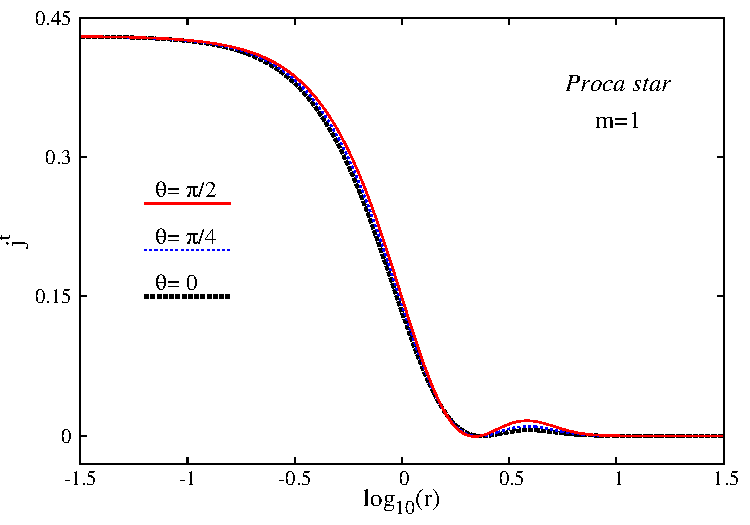
\includegraphics[width=8.1cm]{PS-jt-m1.pdf}
      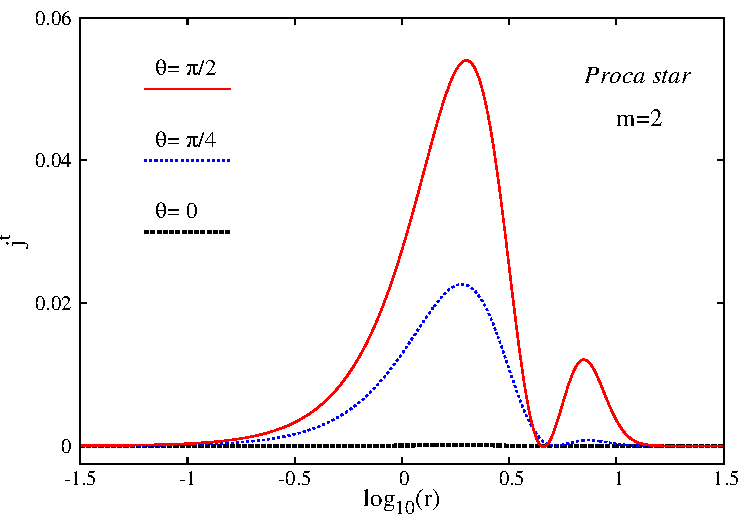
\includegraphics[width=8.1cm]{PS-jt-m2.pdf}
  \end{center}
  \caption{Radial variation of the Noether charge density, $cf.$~\eqref{j}, for different constant $\theta$ sections of the Proca stars exhibited in Fig.~\ref{PS1} (left panel) and Fig.~\ref{PS2} (right panel). One can clearly observe the differences with the angular momentum density.}
  \label{fignc}
\end{figure}
%
For BHs, on the other hand, there is also a horizon contribution which, in general is non-zero:
\begin{equation}
J^{(\mathcal{P})}=mQ+ \oint_\mathcal{H}  P^r dS_r\ .
\label{JQBHs}
\end{equation}  
%%%%%%%%%%%%%%%%%%%%%%%%%%%%%%%%%%%%%%%%%%%%%%%%%


This result  contrasts with that for the scalar boson star case, wherein $T_\varphi^t =m j^t $. The total angular momentum and Noether charge, however, are equal in both cases, for stars. This follows from integrating (\ref{s4}) over a spacelike surface and using the Gauss's theorem:
\begin{eqnarray}
\label{s6}
\int T_\varphi^t \sqrt{-g} d^3 x =m \int j^t \sqrt{-g} d^3 x
+ \oint_\infty  P^r dS_r\ .
\end{eqnarray}
Since the Proca field decays exponentially, the contribution from the $P^r$ term 
is zero and one arrives at (\ref{amnc}).



By using a similar approach, one can easily prove the following identity, where use again the Proca equations (\ref{procafe}) together with
the expressions 
$ {\mathcal{F}}_{\alpha t} =\partial_\alpha {\mathcal{A}}_{t}+i w {\mathcal{A}}_{t}$,
$ \bar{\mathcal{F}}_{\alpha t} =\partial_\alpha \bar{\mathcal{A}}_{t}-i w \bar {\mathcal{A}}_{t}$:
 \begin{equation}
\label{sup1}
T^{\alpha}_\alpha-2T_t^t=
2w j^t - \mu^2 {\mathcal{A}}_\alpha \bar{\mathcal{A}}^\alpha+
\nabla_\alpha U^\alpha,
\end{equation} 
 with
\begin{eqnarray}
\label{sup2}
 U^\alpha=\frac{1}{2} 
\left(
{\mathcal{A}}_\beta \bar{ {\mathcal{F}}}^{\alpha \beta}+\bar{\mathcal{A}}_\beta { {\mathcal{F}}}^{\alpha \beta}
\right)
-\left({\mathcal{A}}_t \bar{ {\mathcal{F}}}^{\alpha t}+\bar{\mathcal{A}}_t { {\mathcal{F}}}^{\alpha t}
\right)  ~.
\end{eqnarray}
For Proca stars,
the integration of the relation (\ref{sup1}) 
over a spacelike surface 
implies the Smarr formula (\ref{smarr-new2}). Here we use again the fact that the Proca field decays exponentially, while the contribution from  $U^r$ at $r=0$ vanishes.

For BHs, however, $U^r$ gives a nontrivial horizon contribution. Then, a combination of (\ref{s4}) and (\ref{sup1}) leads to the simple relation
\begin{eqnarray}
\label{sup3}
\nonumber
&&T^{\alpha}_\alpha-2T_t^t-2\Omega_H T_\varphi^t =	 2(w-\Omega_H m) j^t - \mu^2 {\mathcal{A}}_\alpha \bar{\mathcal{A}}^\alpha \ \ \ \ \ \ \ \ \ \ \ 
\\
&&+
\frac{1}{\sqrt{-g}}
\partial_\alpha 
\bigg[\left(\frac{1}{2} 
\left(
{\mathcal{A}}_\beta \bar{ {\mathcal{F}}}^{\alpha \beta}+\bar{\mathcal{A}}_\beta { {\mathcal{F}}}^{\alpha \beta}
\right)
-\left(
({\mathcal{A}}_t +\Omega_H {\mathcal{A}}_\varphi)\bar{ {\mathcal{F}}}^{\alpha t}
                +
(\bar{\mathcal{A}}_t +\Omega_H \bar{\mathcal{A}}_\varphi){ {\mathcal{F}}}^{\alpha t}
\right)
\right)  
\sqrt{-g} 
\bigg] \ .
\end{eqnarray}
The integration of this identity leads to the simplified 
Smarr formula (\ref{smarr-new1}). Here one uses also the synchronization 
condition (\ref{synchronization}), 
together with  the boundary conditions (\ref{bccloudshorizon}).  


%%%%%%%%%%%%%%%%%%%%%%%%%%%%%%%%%%%%%%%%%%%%%%%%%%%%%%%%%%%%%%%%
\section{Numerical data made available}
\label{appendixd}
%%%%%%%%%%%%%%%%%%%%%%%%%%%%%%%%%%%%%%%%%%%%%%%%%%%%%%%%%%%%%%%%
The following tables detail the information about the four solutions singled out in Fig.~\ref{figdomain}, for each case (Proca and scalar), plus a vacuum Kerr solution that possesses the same ADM mass and angular momentum as configuration III. The numerical data, together with an explanation of its format, is given in  \cite{datakbhph} for the Proca case and in \cite{datakbhsh} for the scalar case.

\bigskip

\begin{center}
\begin{tabular}{|c||c|c|c|c|c|c|c|c|}
\hline
Left panel Fig.~\ref{figdomain} & $w/\mu$  & $r_H/\mu$ & $\mu M_{ADM}$ & $\mu^2J_{ADM}$ & $\mu M_{H}$ & $\mu^2J_{H}$ & $\mu M^{(\mathcal{P})}$ & $\mu^2J^{(\mathcal{P})}$   \\ \hline\hline
I - Proca star  & 0.9 & 0 & 1.456 & 1.45 & 0 & 0 & 1.456 & 1.45 
\\ \hline
II - Vacuum Kerr  & 1.0432 & 0.1945 & 0.365 & 0.128 & 0.365 & 0.128 & 0 & 0
\\ \hline
III - KBHPH & 0.9775 & 0.2475 & 0.365 & 0.128 & 0.354 & 0.117 & 0.011 & 0.011
\\ \hline
IV - KBHPH & 0.863& 0.09 & 0.915 & 0.732 & 0.164 & 0.070 & 0.751 & 0.662
\\ \hline
V - KBHPH & 0.79& 0.06 & 1.173 & 1.079 & 0.035 & 0.006 & 1.138 & 1.073
\\ \hline 
\end{tabular}\\ \bigskip
Table I - Configurations in data publicly available for the Proca case~\cite{datakbhph}.
\end{center}

\bigskip

\begin{center}
\begin{tabular}{|c||c|c|c|c|c|c|c|c|}
\hline
Left panel Fig.~\ref{figdomain} & $w/\mu$  & $r_H/\mu$ & $\mu M_{ADM}$ & $\mu^2J_{ADM}$ & $\mu M_{H}$ & $\mu^2J_{H}$ & $\mu M^{(\Psi)}$ & $\mu^2J^{(\Psi)}$   \\ \hline\hline
I - Scalar boson star  & 0.85 & 0 & 1.25 & 1.30 & 0 & 0 & 1.25 & 1.30 
\\ \hline
II - Vacuum Kerr  & 1.1112 & 0.0663 & 0.415 & 0.172 & 0.415 & 0.172 & 0 & 0
\\ \hline
III - KBHSH & 0.975 & 0.2 & 0.415 & 0.172 & 0.393 & 0.150 & 0.022 & 0.022
\\ \hline
IV - KBHSH & 0.82& 0.1 & 0.933 & 0.739 & 0.234 & 0.114 & 0.699 & 0.625
\\ \hline
V - KBHSH & 0.68& 0.04 & 0.975 & 0.850 & 0.018 & 0.002 & 0.957 & 0.848
\\ \hline 
\end{tabular}\\ \bigskip
Table II - Configurations in data publicly available for the scalar case~\cite{datakbhsh}.
\end{center}


%%%%%%%%%%%%%%%%%%%%%%%%%%%%%%%%%%%%%%%%%%%%%%%%%%%%%%%%%%%%%%%%%%%%%%%%%%%%%%  
\begin{small}
\begin{thebibliography}{99}
%%%%%%%%%%%%%%%%%%%%%%%%%%%%%%%%%%%%%%%%%%%%%%%%%%%%%%%%%%%%%%%%%%%%%%%%%%%%%%  

%\cite{Herdeiro:2014goa}
\bibitem{Herdeiro:2014goa}
  C.~A.~R.~Herdeiro and E.~Radu,
  ``Kerr black holes with scalar hair,''
  Phys.\ Rev.\ Lett.\  {\bf 112} (2014) 221101
  [arXiv:1403.2757 [gr-qc]].
  %%CITATION = ARXIV:1403.2757;%%
  %11 citations counted in INSPIRE as of 21 Jun 2014 
%%%%%%%%%%%%%%%%%%%%%%%%%%%%%%%%%%%%%%%%%%%%%%%%%%%%%%%%%%%%%%%%%%%%%    
  %\cite{Herdeiro:2014ima}
\bibitem{Herdeiro:2014ima}
  C.~A.~R.~Herdeiro and E.~Radu,
  ``A new spin on black hole hair,''
  Int.\ J.\ Mod.\ Phys.\ D {\bf 23} (2014) 12,  1442014
  [arXiv:1405.3696 [gr-qc]].
  %%CITATION = ARXIV:1405.3696;%%
  %17 citations counted in INSPIRE as of 19 Mar 2015
%%%%%%%%%%%%%%%%%%%%%%%%%%%%%%%%%%%%%%%%%%%%%%%%%%%%%%%%%%%%%%%%%%%%%  
%\cite{Brito:2015pxa}
\bibitem{Brito:2015pxa}
  R.~Brito, V.~Cardoso, C.~A.~R.~Herdeiro and E.~Radu,
  ``Proca stars: Gravitating Bose-Einstein condensates of massive spin 1 particles,''
  Phys.\ Lett.\ B {\bf 752} (2016) 291
%  doi:10.1016/j.physletb.2015.11.051
  [arXiv:1508.05395 [gr-qc]].
  %%CITATION = doi:10.1016/j.physletb.2015.11.051;%%
  %3 citations counted in INSPIRE as of 25 Jan 2016
%%%%%%%%%%%%%%%%%%%%%%%%%%%%%%%%%%%%%%%%%%%%%%%%%%%%%%%%%%%%%%%%%%%%%  
%\cite{Carter:1971zc}
\bibitem{Carter:1971zc}
  B.~Carter,
  ``Axisymmetric Black Hole Has Only Two Degrees of Freedom,''
  Phys.\ Rev.\ Lett.\  {\bf 26} (1971) 331.
%  doi:10.1103/PhysRevLett.26.331
  %%CITATION = doi:10.1103/PhysRevLett.26.331;%%
  %444 citations counted in INSPIRE as of 25 Jan 2016
 %%%%%%%%%%%%%%%%%%%%%%%%%%%%%%%%%%%%%%%%%%%%%%%%%%%%%%%%%%%%%%%%%%%%%   
  %\cite{Robinson:1975bv}
\bibitem{Robinson:1975bv}
  D.~C.~Robinson,
  ``Uniqueness of the Kerr black hole,''
  Phys.\ Rev.\ Lett.\  {\bf 34} (1975) 905.
%  doi:10.1103/PhysRevLett.34.905
  %%CITATION = doi:10.1103/PhysRevLett.34.905;%%
  %350 citations counted in INSPIRE as of 25 Jan 2016
 %%%%%%%%%%%%%%%%%%%%%%%%%%%%%%%%%%%%%%%%%%%%%%%%%%%%%%%%%%%%%%%%%%%%%   
  %\cite{Hawking:1971vc}
\bibitem{Hawking:1971vc}
  S.~W.~Hawking,
  ``Black holes in general relativity,''
  Commun.\ Math.\ Phys.\  {\bf 25} (1972) 152.
%  doi:10.1007/BF01877517
  %%CITATION = doi:10.1007/BF01877517;%%
  %587 citations counted in INSPIRE as of 25 janv. 2016
%%%%%%%%%%%%%%%%%%%%%%%%%%%%%%%%%%%%%%%%%%%%%%%%%%%%%%%%%%%%%%%%%%%%%  
%\cite{Racz:1995nh}
\bibitem{Racz:1995nh}
  I.~Racz and R.~M.~Wald,
  ``Global extensions of space-times describing asymptotic final states of black holes,''
  Class.\ Quant.\ Grav.\  {\bf 13} (1996) 539
%  doi:10.1088/0264-9381/13/3/017
  [gr-qc/9507055].
  %%CITATION = doi:10.1088/0264-9381/13/3/017;%%
  %76 citations counted in INSPIRE as of 25 janv. 2016
 %%%%%%%%%%%%%%%%%%%%%%%%%%%%%%%%%%%%%%%%%%%%%%%%%%%%%%%%%%%%%%%%%%%%%   
  %\cite{Robinson:2004zz}
%\bibitem{Robinson:2004zz}
 % D.~Robinson,
%  ``Four decades of black holes uniqueness theorems,''
  %%CITATION = INSPIRE-673719;%%
  %3 citations counted in INSPIRE as of 25 janv. 2016

  %%%%%%%%%%%%%%%%%%%%%%%%%%%%%%%%%%%%%%%%%%%%%%%%%%%%%
%\cite{Chrusciel:2012jk}
\bibitem{Chrusciel:2012jk}
  P.~T.~Chrusciel, J.~L.~Costa and M.~Heusler,
  ``Stationary Black Holes: Uniqueness and Beyond,''
  Living Rev.\ Rel.\  {\bf 15} (2012) 7
%  doi:10.12942/lrr-2012-7
  [arXiv:1205.6112 [gr-qc]].
  %%CITATION = doi:10.12942/lrr-2012-7;%%
  %80 citations counted in INSPIRE as of 25 janv. 2016
   %%%%%%%%%%%%%%%%%%%%%%%%%%%%%%%%%%%%%%%%%%%%%%%%%%%%% 
  %\cite{Kerr:1963ud}
\bibitem{Kerr:1963ud}
  R.~P.~Kerr,
  ``Gravitational field of a spinning mass as an example of algebraically special metrics,''
  Phys.\ Rev.\ Lett.\  {\bf 11} (1963) 237.
%  doi:10.1103/PhysRevLett.11.237
  %%CITATION = doi:10.1103/PhysRevLett.11.237;%%
  %870 citations counted in INSPIRE as of 25 Jan 2016
   %%%%%%%%%%%%%%%%%%%%%%%%%%%%%%%%%%%%%%%%%%%%%%%%%%%%% 
  %\cite{Ruffini:1971bza}
\bibitem{Ruffini:1971bza}
  R.~Ruffini and J.~A.~Wheeler,
  ``Introducing the black hole,''
  Phys.\ Today {\bf 24} (1971) 1,  30.
%  doi:10.1063/1.3022513
  %%CITATION = doi:10.1063/1.3022513;%%
  %178 citations counted in INSPIRE as of 25 Jan 2016
  %%%%%%%%%%%%%%%%%%%%%%%%%%%%%%%%%%%%%%%%%%%%%%%%%%%%%
%\cite{Herdeiro:2015waa}
\bibitem{Herdeiro:2015waa}
  C.~A.~R.~Herdeiro and E.~Radu,
  ``Asymptotically flat black holes with scalar hair: a review,''
  Int.\ J.\ Mod.\ Phys.\ D {\bf 24} (2015) 09,  1542014
%  doi:10.1142/S0218271815420146
  [arXiv:1504.08209 [gr-qc]].
  %%CITATION = doi:10.1142/S0218271815420146;%%
  %24 citations counted in INSPIRE as of 25 janv. 2016
    %%%%%%%%%%%%%%%%%%%%%%%%%%%%%%%%%%%%%%%%%%%%%%%%%%%%%
  %\cite{Bekenstein:1971hc}
\bibitem{Bekenstein:1971hc}
  J.~D.~Bekenstein,
  ``Nonexistence of baryon number for static black holes,''
  Phys.\ Rev.\ D {\bf 5} (1972) 1239.
%  doi:10.1103/PhysRevD.5.1239
  %%CITATION = doi:10.1103/PhysRevD.5.1239;%%
  %321 citations counted in INSPIRE as of 25 janv. 2016
  %%%%%%%%%%%%%%%%%%%%%%%%%%%%%%%%%%%%%%%%%%%%%%%%%%%%%
%\cite{Bekenstein:1972ky}
\bibitem{Bekenstein:1972ky}
  J.~D.~Bekenstein,
  ``Nonexistence of baryon number for black holes. ii,''
  Phys.\ Rev.\ D {\bf 5} (1972) 2403.
%  doi:10.1103/PhysRevD.5.2403
  %%CITATION = doi:10.1103/PhysRevD.5.2403;%%
  %168 citations counted in INSPIRE as of 25 janv. 2016
  
  %%%%%%%%%%%%%%%%%%%%%%%%%%%%%%%%%%%%%%%%%%%%%%%%%%%%%
%\cite{Volkov:1998cc}
\bibitem{Volkov:1998cc}
  M.~S.~Volkov and D.~V.~Gal'tsov,
  ``Gravitating non-Abelian solitons and black holes with Yang-Mills fields,''
  Phys.\ Rept.\  {\bf 319} (1999) 1
  [hep-th/9810070].
  %%CITATION = HEP-TH/9810070;%%
  %239 citations counted in INSPIRE as of 11 Apr 2015
  %%%%%%%%%%%%%%%%%%%  

%\cite{Bizon:1994dh}
\bibitem{Bizon:1994dh}
  P.~Bizon,
  ``Gravitating solitons and hairy black holes,''
  Acta Phys.\ Polon.\ B {\bf 25} (1994) 877
  [gr-qc/9402016].
  %%CITATION = GR-QC/9402016;%%
  %42 citations counted in INSPIRE as of 25 janv. 2016
  %%%%%%%%%%%%%%%%%%%%%%%%%%%%%%%%%%%%%%%%%%%%%%%%%%%%%
%\cite{Bekenstein:1996pn}
\bibitem{Bekenstein:1996pn}
  J.~D.~Bekenstein,
  ``Black hole hair: 25 - years after,''
  In "`Moscow 1996, 2nd International A.D. Sakharov Conference on physics"', pp. 216-219
  [gr-qc/9605059].
  %%CITATION = GR-QC/9605059;%%
  %83 citations counted in INSPIRE as of 25 janv. 2016
  %%%%%%%%%%%%%%%%%%%%%%%%%%%%%%%%%%%%%%%%%%%%%%%%%%%%%
%\cite{Volkov:2016ehx}
\bibitem{Volkov:2016ehx}
  M.~S.~Volkov,
  ``Hairy black holes in the XX-th and XXI-st centuries,''
  arXiv:1601.08230 [gr-qc].
  %%CITATION = ARXIV:1601.08230;%%
  %%%%%%%%%%%%%%%%%%%%%%%%%%%%%%%%%%%%%%%%%%%%%%%%%%%%%
 
%\cite{Nucamendi:1995ex}
\bibitem{Nucamendi:1995ex}
  U.~Nucamendi and M.~Salgado,
  ``Scalar hairy black holes and solitons in asymptotically flat space-times,''
  Phys.\ Rev.\ D {\bf 68} (2003) 044026
  [gr-qc/0301062].
  %%CITATION = GR-QC/0301062;%%
  %38 citations counted in INSPIRE as of 31 Mar 2015  
  %%%%%%%%%%%%%%%%%%%%%%%%%%%%%%%%%%%%%%%%%%%%%%%%%%%%%

%\cite{Bechmann:1995sa}
\bibitem{Bechmann:1995sa}
  O.~Bechmann and O.~Lechtenfeld,
  ``Exact black hole solution with selfinteracting scalar field,''
  Class.\ Quant.\ Grav.\  {\bf 12} (1995) 1473
  [gr-qc/9502011].
  %%CITATION = GR-QC/9502011;%%
  %28 citations counted in INSPIRE as of 31 Mar 2015
  %%%%%%%%%%%%%%%%%%%%%%%%%%%%%%%%%%%%%%%%%%%%%%%%%%%%%
%\cite{Anabalon:2013qua}
\bibitem{Anabalon:2013qua}
  A.~Anabalon, D.~Astefanesei and R.~Mann,
  ``Exact asymptotically flat charged hairy black holes with a dilaton potential,''
  JHEP {\bf 1310} (2013) 184
  [arXiv:1308.1693 [hep-th]].
  %%CITATION = ARXIV:1308.1693;%%
  %14 citations counted in INSPIRE as of 31 Mar 2015
 %%%%%%%%%%%%%%%%%%%%%%%%%%%%%%%%%%%%%%%%%%%%%%%%%%%%%
%\cite{Anabalon:2012ih}
\bibitem{Anabalon:2012ih}
  A.~Anabalon and J.~Oliva,
  ``Exact Hairy Black Holes and their Modification to the Universal Law of Gravitation,''
  Phys.\ Rev.\ D {\bf 86} (2012) 107501
  [arXiv:1205.6012 [gr-qc]].
  %%CITATION = ARXIV:1205.6012;%%
  %15 citations counted in INSPIRE as of 31 Mar 2015  
 %%%%%%%%%%%%%%%%%%%%%%%%%%%%%%%%%%%%%%%%%%%%%%%%%%%%%
%\cite{Cadoni:2015gfa}
\bibitem{Cadoni:2015gfa}
  M.~Cadoni and E.~Franzin,
  ``Asymptotically flat black holes sourced by a massless scalar field,''
  arXiv:1503.04734 [gr-qc].
  %%CITATION = ARXIV:1503.04734;%%  

 %%%%%%%%%%%%%%%%%%%%%%%%%%%%%%%%%%%%%%%%%%%%%%%%%%%%%

%\cite{Bekenstein:1975ts}
\bibitem{Bekenstein:1975ts}
  J.~D.~Bekenstein,
  ``Black Holes with Scalar Charge,''
  Annals Phys.\  {\bf 91} (1975) 75.
  %%CITATION = APNYA,91,75;%%
  %103 citations counted in INSPIRE as of 26 mar 2015

 %%%%%%%%%%%%%%%%%%%%%%%%%%%%%%%%%%%%%%%%%%%%%%%%%%%%%
%\cite{Bekenstein:1974sf}
\bibitem{Bekenstein:1974sf}
  J.~D.~Bekenstein,
  ``Exact solutions of Einstein conformal scalar equations,''
  Annals Phys.\  {\bf 82} (1974) 535.
  %%CITATION = APNYA,82,535;%%
  %231 citations counted in INSPIRE as of 26 Mar 2015
 %%%%%%%%%%%%%%%%%%%%%%%%%%%%%%%%%%%%%%%%%%%%%%%%%%%%%
\bibitem{BBM}
N.~M.~Bocharova, K.~A.~Bronnikov, V.~N.~Melnikov,
Vestn. Mosk. Univ. Fiz. Astron. {\bf 6} (1970) 706. 
 %%%%%%%%%%%%%%%%%%%%%%%%%%%%%%%%%%%%%%%%%%%%%%%%%%%%%
%\cite{Sotiriou:2014pfa}
\bibitem{Sotiriou:2014pfa}
  T.~P.~Sotiriou and S.~Y.~Zhou,
  ``Black hole hair in generalized scalar-tensor gravity: An explicit example,''
  Phys.\ Rev.\ D {\bf 90} (2014) 12,  124063
  [arXiv:1408.1698 [gr-qc]].
  %%CITATION = ARXIV:1408.1698;%%
  %7 citations counted in INSPIRE as of 30 Mar 2015
 %%%%%%%%%%%%%%%%%%%%%%%%%%%%%%%%%%%%%%%%%%%%%%%%%%%%%
%\cite{Sotiriou:2013qea}
\bibitem{Sotiriou:2013qea}
  T.~P.~Sotiriou and S.~Y.~Zhou,
  ``Black hole hair in generalized scalar-tensor gravity,''
  Phys.\ Rev.\ Lett.\  {\bf 112} (2014) 251102
  [arXiv:1312.3622 [gr-qc]].
  %%CITATION = ARXIV:1312.3622;%%
  %19 citations counted in INSPIRE as of 30 Mar 2015
   %%%%%%%%%%%%%%%%%%%%%%%%%%%%%%%%%%%%%%%%%%%%%%%%%%%%%
  %\cite{Babichev:2013cya}
\bibitem{Babichev:2013cya}
  E.~Babichev and C.~Charmousis,
  ``Dressing a black hole with a time-dependent Galileon,''
  JHEP {\bf 1408} (2014) 106
  [arXiv:1312.3204 [gr-qc]].
  %%CITATION = ARXIV:1312.3204;%%
  %23 citations counted in INSPIRE as of 30 Mar 2015
   %%%%%%%%%%%%%%%%%%%%%%%%%%%%%%%%%%%%%%%%%%%%%%%%%%%%%
  %\cite{Luckock:1986tr}
\bibitem{Luckock:1986tr}
  H.~Luckock and I.~Moss,
  ``Black Holes Have Skyrmion Hair,''
  Phys.\ Lett.\ B {\bf 176} (1986) 341.
  %%CITATION = PHLTA,B176,341;%%
  %52 citations counted in INSPIRE as of 31 Mar 2015   
 %%%%%%%%%%%%%%%%%%%%%%%%%%%%%%%%%%%%%%%%%%%%%%%%%%%%%
%\cite{Luckock}
\bibitem{Luckock}
H. Luckock, {\it Black hole skyrmions}, in H.J. De Vega and N. Sanches, editors,
{\it String Theory, Quantum Cosmology and Quantum Gravity, Integrable and
Conformal Integrable Theories} pp. 455, World Scientific, 1987. 

 %%%%%%%%%%%%%%%%%%%%%%%%%%%%%%%%%%%%%%%%%%%%%%%%%%%%%
%\cite{Bronnikov:2005gm}
\bibitem{Bronnikov:2005gm}
  K.~A.~Bronnikov and J.~C.~Fabris,
  ``Regular phantom black holes,''
  Phys.\ Rev.\ Lett.\  {\bf 96} (2006) 251101
  [gr-qc/0511109].
  %%CITATION = GR-QC/0511109;%%
 %%%%%%%%%%%%%%%%%%%%%%%%%%%%%%%%%%%%%%%%%%%%%%%%%%%%%	
	%\cite{Radu:2011uj}
\bibitem{Radu:2011uj}
  E.~Radu, Y.~Shnir and D.~H.~Tchrakian,
  ``Scalar hairy black holes and solitons in a gravitating Goldstone model,''
  Phys.\ Lett.\ B {\bf 703} (2011) 386
 % doi:10.1016/j.physletb.2011.08.032
  [arXiv:1106.5066 [gr-qc]].
  %%CITATION = doi:10.1016/j.physletb.2011.08.032;%%
  %2 citations counted in INSPIRE as of 05 Mar 2016
	
 %%%%%%%%%%%%%%%%%%%%%%%%%%%%%%%%%%%%%%%%%%%%%%%%%%%%%
%\cite{Gibbons:1987ps}
\bibitem{Gibbons:1987ps}
  G.~W.~Gibbons and K.~i.~Maeda,
  ``Black Holes and Membranes in Higher Dimensional Theories with Dilaton Fields,''
  Nucl.\ Phys.\ B {\bf 298} (1988) 741.
  %%CITATION = NUPHA,B298,741;%%
  %938 citations counted in INSPIRE as of 26 mar 2015
 %%%%%%%%%%%%%%%%%%%%%%%%%%%%%%%%%%%%%%%%%%%%%%%%%%%%%
%\cite{Gibbons:1982ih}
\bibitem{Gibbons:1982ih}
  G.~W.~Gibbons,
  ``Antigravitating Black Hole Solitons with Scalar Hair in N=4 Supergravity,''
  Nucl.\ Phys.\ B {\bf 207} (1982) 337.
  %%CITATION = NUPHA,B207,337;%%
  %337 citations counted in INSPIRE as of 26 Mar 2015
%%%%%%%%%%%%%%%%%%%%%%%%%%%%%%%%%%%%%%%%%%%%%%%%%%%%%%%%%%%%%%%%%%%%%%%%

%\cite{Kanti:1995vq}Ayzenberg:2014aka}Kleihaus:2011tg}Pani:2011gy}Pani:2009wy}Alexander:2009tp}{Yunes:2009hc}
\bibitem{Kanti:1995vq}
  P.~Kanti, N.~E.~Mavromatos, J.~Rizos, K.~Tamvakis and E.~Winstanley,
  ``Dilatonic black holes in higher curvature string gravity,''
  Phys.\ Rev.\ D {\bf 54} (1996) 5049
  [hep-th/9511071].
  %%CITATION = HEP-TH/9511071;%%
  %112 citations counted in INSPIRE as of 31 Mar 2015
 %%%%%%%%%%%%%%%%%%%%%%%%%%%%%%%%%%%%%%%%%%%%%%%%%%%%%
%\cite{Ayzenberg:2014aka}
\bibitem{Ayzenberg:2014aka}
  D.~Ayzenberg and N.~Yunes,
  ``Slowly-Rotating Black Holes in Einstein-Dilaton-Gauss-Bonnet Gravity: Quadratic Order in Spin Solutions,''
  Phys.\ Rev.\ D {\bf 90} (2014) 044066
   [Erratum-ibid.\ D {\bf 91} (2015) 6,  069905]
  [arXiv:1405.2133 [gr-qc]].
  %%CITATION = ARXIV:1405.2133;%%
  %7 citations counted in INSPIRE as of 31 Mar 2015  
 %%%%%%%%%%%%%%%%%%%%%%%%%%%%%%%%%%%%%%%%%%%%%%%%%%%%%
%\cite{Kleihaus:2011tg}
\bibitem{Kleihaus:2011tg}
  B.~Kleihaus, J.~Kunz and E.~Radu,
  ``Rotating Black Holes in Dilatonic Einstein-Gauss-Bonnet Theory,''
  Phys.\ Rev.\ Lett.\  {\bf 106} (2011) 151104
  [arXiv:1101.2868 [gr-qc]].
  %%CITATION = ARXIV:1101.2868;%%
  %22 citations counted in INSPIRE as of 31 Mar 2015  
 %%%%%%%%%%%%%%%%%%%%%%%%%%%%%%%%%%%%%%%%%%%%%%%%%%%%%
%\cite{Kleihaus:2015aje}
\bibitem{Kleihaus:2015aje}
  B.~Kleihaus, J.~Kunz, S.~Mojica and E.~Radu,
  ``Spinning black holes in Einstein?Gauss-Bonnet?dilaton theory: Nonperturbative solutions,''
  Phys.\ Rev.\ D {\bf 93} (2016) 4,  044047
  %doi:10.1103/PhysRevD.93.044047
  [arXiv:1511.05513 [gr-qc]].
  %%CITATION = doi:10.1103/PhysRevD.93.044047;%%
  %4 citations counted in INSPIRE as of 05 Mar 2016
 %%%%%%%%%%%%%%%%%%%%%%%%%%%%%%%%%%%%%%%%%%%%%%%%%%%%%

%\cite{Pani:2011gy}
\bibitem{Pani:2011gy}
  P.~Pani, C.~F.~B.~Macedo, L.~C.~B.~Crispino and V.~Cardoso,
  ``Slowly rotating black holes in alternative theories of gravity,''
  Phys.\ Rev.\ D {\bf 84} (2011) 087501
  [arXiv:1109.3996 [gr-qc]].
  %%CITATION = ARXIV:1109.3996;%%
  %29 citations counted in INSPIRE as of 24 Apr 2015
 %%%%%%%%%%%%%%%%%%%%%%%%%%%%%%%%%%%%%%%%%%%%%%%%%%%%%
%\cite{Pani:2009wy}
\bibitem{Pani:2009wy}
  P.~Pani and V.~Cardoso,
  ``Are black holes in alternative theories serious astrophysical candidates? The Case for Einstein-Dilaton-Gauss-Bonnet black holes,''
  Phys.\ Rev.\ D {\bf 79} (2009) 084031
  [arXiv:0902.1569 [gr-qc]].
  %%CITATION = ARXIV:0902.1569;%%
  %43 citations counted in INSPIRE as of 24 Apr 2015
 %%%%%%%%%%%%%%%%%%%%%%%%%%%%%%%%%%%%%%%%%%%%%%%%%%%%%
%\cite{Alexander:2009tp}
\bibitem{Alexander:2009tp}
  S.~Alexander and N.~Yunes,
  ``Chern-Simons Modified General Relativity,''
  Phys.\ Rept.\  {\bf 480} (2009) 1
  [arXiv:0907.2562 [hep-th]].
  %%CITATION = ARXIV:0907.2562;%%
  %143 citations counted in INSPIRE as of 31 Mar 2015
 %%%%%%%%%%%%%%%%%%%%%%%%%%%%%%%%%%%%%%%%%%%%%%%%%%%%%

%\cite{Yunes:2009hc}
\bibitem{Yunes:2009hc}
  N.~Yunes and F.~Pretorius,
  ``Dynamical Chern-Simons Modified Gravity. I. Spinning Black Holes in the Slow-Rotation Approximation,''
  Phys.\ Rev.\ D {\bf 79} (2009) 084043
  [arXiv:0902.4669 [gr-qc]].
  %%CITATION = ARXIV:0902.4669;%%
  %96 citations counted in INSPIRE as of 31 Mar 2015  
 %%%%%%%%%%%%%%%%%%%%%%%%%%%%%%%%%%%%%%%%%%%%%%%%%%%%%
 
  %\cite{Schunck:2003kk}
\bibitem{Schunck:2003kk}
  F.~E.~Schunck and E.~W.~Mielke,
  ``General relativistic boson stars,''
  Class.\ Quant.\ Grav.\  {\bf 20} (2003) R301
  [arXiv:0801.0307 [astro-ph]].
  %%CITATION = ARXIV:0801.0307;%%
  %125 citations counted in INSPIRE as of 17 Mar 2015
 %%%%%%%%%%%%%%%%%%%%%%%%%%%%%%%%%%%%%%%%%%%%%%%%%%%%%
%\cite{Liebling:2012fv}
\bibitem{Liebling:2012fv}
  S.~L.~Liebling and C.~Palenzuela,
  ``Dynamical Boson Stars,''
  Living Rev.\ Rel.\  {\bf 15} (2012) 6
  [arXiv:1202.5809 [gr-qc]].
  %%CITATION = ARXIV:1202.5809;%%
  %12 citations counted in INSPIRE as of 18 Jun 2013 
   %%%%%%%%%%%%%%%%%%%%%%%%%%%%%%%%%%%%%%%%%%%%%%%%%%%%%
  %\cite{Herdeiro:2015gia}
\bibitem{Herdeiro:2015gia}
  C.~Herdeiro and E.~Radu,
  ``Construction and physical properties of Kerr black holes with scalar hair,''
  Class.\ Quant.\ Grav.\  {\bf 32} (2015) 14,  144001
  [arXiv:1501.04319 [gr-qc]].
  %%CITATION = ARXIV:1501.04319;%%
  %23 citations counted in INSPIRE as of 26 ao?t 2015
   %%%%%%%%%%%%%%%%%%%%%%%%%%%%%%%%%%%%%%%%%%%%%%%%%%%%%
  %\cite{Press:1972zz}
\bibitem{Press:1972zz}
  W.~H.~Press and S.~A.~Teukolsky,
  ``Floating Orbits, Superradiant Scattering and the Black-hole Bomb,''
  Nature {\bf 238} (1972) 211.
%  doi:10.1038/238211a0
  %%CITATION = doi:10.1038/238211a0;%%
  %224 citations counted in INSPIRE as of 25 Jan 2016
 %%%%%%%%%%%%%%%%%%%%%%%%%%%%%%%%%%%%%%%%%%%%%%%%%%%%%
%\cite{Damour:1976kh}
\bibitem{Damour:1976kh}
  T.~Damour, N.~Deruelle and R.~Ruffini,
  ``On Quantum Resonances in Stationary Geometries,''
  Lett.\ Nuovo Cim.\  {\bf 15} (1976) 257.
 % doi:10.1007/BF02725534
  %%CITATION = doi:10.1007/BF02725534;%%
  %116 citations counted in INSPIRE as of 25 janv. 2016
 %%%%%%%%%%%%%%%%%%%%%%%%%%%%%%%%%%%%%%%%%%%%%%%%%%%%%
%\cite{Brito:2015oca}
\bibitem{Brito:2015oca}
  R.~Brito, V.~Cardoso and P.~Pani,
  ``Superradiance,''
  Lect.\ Notes Phys.\  {\bf 906} (2015) pp.1
%  doi:10.1007/978-3-319-19000-6
  [arXiv:1501.06570 [gr-qc]].
  %%CITATION = doi:10.1007/978-3-319-19000-6;%%
  %44 citations counted in INSPIRE as of 25 Jan 2016
 %%%%%%%%%%%%%%%%%%%%%%%%%%%%%%%%%%%%%%%%%%%%%%%%%%%%%
  
  %\cite{Hod:2012px}Hod:2013zza}Hod:2014baa}Benone:2014ssa}Hod:2014npa}Hod:2015ota}
\bibitem{Hod:2012px}
  S.~Hod,
  ``Stationary Scalar Clouds Around Rotating Black Holes,''
  Phys.\ Rev.\ D {\bf 86} (2012) 104026
   [Erratum-ibid.\ D {\bf 86} (2012) 129902]
  [arXiv:1211.3202 [gr-qc]].
  %%CITATION = ARXIV:1211.3202;%%
  %30 citations counted in INSPIRE as of 19 mar 2015
  %%%%%%%%%%%%%%%%%%%%%%%%%%%%%%%%%%%%%%%%%%%%%%%%%%%%% 
  %\cite{Hod:2013zza}
\bibitem{Hod:2013zza}
  S.~Hod,
  ``Stationary resonances of rapidly-rotating Kerr black holes,''
  Eur.\ Phys.\ J.\ C {\bf 73} (2013) 4,  2378
  [arXiv:1311.5298 [gr-qc]].
  %%CITATION = ARXIV:1311.5298;%%
  %19 citations counted in INSPIRE as of 19 mar 2015
  %%%%%%%%%%%%%%%%%%%%%%%%%%%%%%%%%%%%%%%%%%%%%%%%%%%%% 
  %\cite{Hod:2014baa}
\bibitem{Hod:2014baa}
  S.~Hod,
  ``Kerr-Newman black holes with stationary charged scalar clouds,''
  Phys.\ Rev.\ D {\bf 90} (2014) 2,  024051
  [arXiv:1406.1179 [gr-qc]].
  %%CITATION = ARXIV:1406.1179;%%
  %10 citations counted in INSPIRE as of 19 Mar 2015
 %%%%%%%%%%%%%%%%%%%%%%%%%%%%%%%%%%%%%%%%%%%%%%%%%%%%%
%\cite{Benone:2014ssa}
\bibitem{Benone:2014ssa}
  C.~L.~Benone, L.~C.~B.~Crispino, C.~Herdeiro and E.~Radu,
  ``Kerr-Newman scalar clouds,''
  Phys.\ Rev.\ D {\bf 90} (2014) 10,  104024
  [arXiv:1409.1593 [gr-qc]].
  %%CITATION = ARXIV:1409.1593;%%
  %8 citations counted in INSPIRE as of 19 Mar 2015
   %%%%%%%%%%%%%%%%%%%%%%%%%%%%%%%%%%%%%%%%%%%%%%%%%%%%%
  %\cite{Hod:2014npa}
\bibitem{Hod:2014npa}
  S.~Hod,
  ``Rotating black holes can have short bristles,''
  Phys.\ Lett.\ B {\bf 739} (2014) 196
  [arXiv:1411.2609 [gr-qc]].
  %%CITATION = ARXIV:1411.2609;%%
  %5 citations counted in INSPIRE as of 19 Mar 2015
   %%%%%%%%%%%%%%%%%%%%%%%%%%%%%%%%%%%%%%%%%%%%%%%%%%%%%
  %\cite{Hod:2015ota}
\bibitem{Hod:2015ota}
  S.~Hod,
  ``The large-mass limit of cloudy black holes,''
  Class.\ Quant.\ Grav.\  {\bf 32} (2015) 13,  134002.
  %%CITATION = CQGRD,32,134002;%%

 %%%%%%%%%%%%%%%%%%%%%%%%%%%%%%%%%%%%%%%%%%%%%%%%%%%%%
  
  %\cite{Sanchis-Gual:2015lje}
\bibitem{Sanchis-Gual:2015lje}
  N.~Sanchis-Gual, J.~C.~Degollado, P.~J.~Montero, J.~A.~Font and C.~Herdeiro,
  ``Explosion and final state of the charged black hole bomb,''
  arXiv:1512.05358 [gr-qc].
  %%CITATION = ARXIV:1512.05358;%%
  %1 citations counted in INSPIRE as of 25 Jan 2016
 %%%%%%%%%%%%%%%%%%%%%%%%%%%%%%%%%%%%%%%%%%%%%%%%%%%%%
%\cite{Bosch:2016vcp}
\bibitem{Bosch:2016vcp}
  P.~Bosch, S.~R.~Green and L.~Lehner,
  ``Nonlinear evolution and final fate of (charged) superradiant instability,''
  arXiv:1601.01384 [gr-qc].
  %%CITATION = ARXIV:1601.01384;%%
 %%%%%%%%%%%%%%%%%%%%%%%%%%%%%%%%%%%%%%%%%%%%%%%%%%%%%
%\cite{Chodosh:2015oma}
\bibitem{Chodosh:2015oma}
  O.~Chodosh and Y.~Shlapentokh-Rothman,
  ``Time-Periodic Einstein-Klein-Gordon Bifurcations of Kerr,''
  arXiv:1510.08025 [gr-qc].
  %%CITATION = ARXIV:1510.08025;%%
  %1 citations counted in INSPIRE as of 25 Jan 2016

 %%%%%%%%%%%%%%%%%%%%%%%%%%%%%%%%%%%%%%%%%%%%%%%%%%%%%
%\cite{Herdeiro:2015tia}
\bibitem{Herdeiro:2015tia}
  C.~A.~R.~Herdeiro, E.~Radu and H.~R?narsson,
  ``Kerr black holes with self-interacting scalar hair: hairier but not heavier,''
  Phys.\ Rev.\ D {\bf 92} (2015) 8,  084059
%  doi:10.1103/PhysRevD.92.084059
  [arXiv:1509.02923 [gr-qc]].
  %%CITATION = doi:10.1103/PhysRevD.92.084059;%%
  %3 citations counted in INSPIRE as of 06 Dec 2015
   %%%%%%%%%%%%%%%%%%%%%%%%%%%%%%%%%%%%%%%%%%%%%%%%%%%%%
  %\cite{Kleihaus:2015iea}
\bibitem{Kleihaus:2015iea}
  B.~Kleihaus, J.~Kunz and S.~Yazadjiev,
  ``Scalarized Hairy Black Holes,''
  Phys.\ Lett.\ B {\bf 744} (2015) 406
%  doi:10.1016/j.physletb.2015.04.014
  [arXiv:1503.01672 [gr-qc]].
  %%CITATION = doi:10.1016/j.physletb.2015.04.014;%%
  %6 citations counted in INSPIRE as of 25 janv. 2016
 %%%%%%%%%%%%%%%%%%%%%%%%%%%%%%%%%%%%%%%%%%%%%%%%%%%%%

%\cite{Pani:2012vp}
\bibitem{Pani:2012vp}
  P.~Pani, V.~Cardoso, L.~Gualtieri, E.~Berti and A.~Ishibashi,
  ``Black hole bombs and photon mass bounds,''
  Phys.\ Rev.\ Lett.\  {\bf 109} (2012) 131102
  [arXiv:1209.0465 [gr-qc]].
  %%CITATION = ARXIV:1209.0465;%%
  %63 citations counted in INSPIRE as of 25 Oct 2015
   %%%%%%%%%%%%%%%%%%%%%%%%%%%%%%%%%%%%%%%%%%%%%%%%%%%%%
  %\cite{Pani:2012bp}
\bibitem{Pani:2012bp}
  P.~Pani, V.~Cardoso, L.~Gualtieri, E.~Berti and A.~Ishibashi,
  ``Perturbations of slowly rotating black holes: massive vector fields in the Kerr metric,''
  Phys.\ Rev.\ D {\bf 86} (2012) 104017
%  doi:10.1103/PhysRevD.86.104017
  [arXiv:1209.0773 [gr-qc]].
  %%CITATION = doi:10.1103/PhysRevD.86.104017;%%
  %41 citations counted in INSPIRE as of 25 Jan 2016

   %%%%%%%%%%%%%%%%%%%%%%%%%%%%%%%%%%%%%%%%%%%%%%%%%%%%%
  %\cite{Witek:2012tr}
\bibitem{Witek:2012tr}
  H.~Witek, V.~Cardoso, A.~Ishibashi and U.~Sperhake,
  ``Superradiant instabilities in astrophysical systems,''
  Phys.\ Rev.\ D {\bf 87} (2013) 4,  043513
%  doi:10.1103/PhysRevD.87.043513
  [arXiv:1212.0551 [gr-qc]].
  %%CITATION = doi:10.1103/PhysRevD.87.043513;%%
  %64 citations counted in INSPIRE as of 25 Jan 2016 
%%%%%%%%%%%%%%%%%%%%%%%%%%%%%%%%%%%%%%%%%%%%%%%%%%%%%%%%%%%%
%\cite{Greene:1992fw}
\bibitem{Greene:1992fw}
  B.~R.~Greene, S.~D.~Mathur and C.~M.~O'Neill,
  ``Eluding the no hair conjecture: Black holes in spontaneously broken gauge theories,''
  Phys.\ Rev.\ D {\bf 47} (1993) 2242
%  doi:10.1103/PhysRevD.47.2242
  [hep-th/9211007].
  %%CITATION = doi:10.1103/PhysRevD.47.2242;%%
  %90 citations counted in INSPIRE as of 17 Feb 2016
 %%%%%%%%%%%%%%%%%%%%%%%%%%%%%%%%%%%%%%%%%%%%%%%%%%%%% 
%\cite{Pena:1997cy}
\bibitem{Pena:1997cy}
  I.~Pena and D.~Sudarsky,
  ``Do collapsed boson stars result in new types of black holes?,''
  Class.\ Quant.\ Grav.\  {\bf 14} (1997) 3131.
  %%CITATION = CQGRD,14,3131;%%
  %31 citations counted in INSPIRE as of 25 Oct 2015
 %%%%%%%%%%%%%%%%%%%%%%%%%%%%%%%%%%%%%%%%%%%%%%%%%%%%%
  \bibitem{Proca}
A.~Proca,   
``Th\'eorie non relativiste des particules  \'a spin entier,''
J. Phys. Radium 9 (1938) 61.
 %%%%%%%%%%%%%%%%%%%%%%%%%%%%%%%%%%%%%%%%%%%%%%%%%%%%%
\bibitem{Rosen:1994rq}
  N.~Rosen,
  ``A Classical Proca particle,''
  Found.\ Phys.\  {\bf 24} (1994) 1689.
  %%CITATION = FNDPA,24,1689;%%
  %4 citations counted in INSPIRE as of 28 Sep 2015
 %%%%%%%%%%%%%%%%%%%%%%%%%%%%%%%%%%%%%%%%%%%%%%%%%%%%%
  %\cite{Obukhov:1999ed} 
\bibitem{Obukhov:1999ed}
  Y.~N.~Obukhov and E.~J.~Vlachynsky,
  ``Einstein-Proca model: Spherically symmetric solutions,''
  Annals Phys.\  {\bf 8} (1999) 497
  [gr-qc/0004081].
  %%CITATION = GR-QC/0004081;%%
  %7 citations counted in INSPIRE as of 28 Sep 2015 
  %%%%%%%%%%%%%%%%%%%%%%%%%%%%%%%%%%%%%%%%%%%%%%%%%%%%%	
%\cite{Toussaint:1999zz}
\bibitem{Toussaint:1999zz}
  M.~Toussaint,
  ``A numeric solution for Einstein's gravitational theory with Proca matter and metric-affine gravity,''
  Gen.\ Rel.\ Grav.\  {\bf 32} (2000) 1689
  [gr-qc/9910042].
  %%CITATION = GR-QC/9910042;%%
  %3 citations counted in INSPIRE as of 28 Sep 2015	
 %%%%%%%%%%%%%%%%%%%%%%%%%%%%%%%%%%%%%%%%%%%%%%%%%%%%%
%\cite{Vuille:2002qz}
\bibitem{Vuille:2002qz}
  C.~Vuille, J.~Ipser and J.~Gallagher,
  ``Einstein-Proca model, micro black holes, and naked singularities,''
  Gen.\ Rel.\ Grav.\  {\bf 34} (2002) 689.
  %%CITATION = GRGVA,34,689;%%
  %5 citations counted in INSPIRE as of 28 Sep 2015	
 %%%%%%%%%%%%%%%%%%%%%%%%%%%%%%%%%%%%%%%%%%%%%%%%%%%%%
 %\cite{Gottlieb:1984jg}
\bibitem{Gottlieb:1984jg}
  D.~Gottlieb, R.~Hojman, L.~H.~Rodriguez and N.~Zamorano,
  ``Yukawa Potential In A Schwarzschild Background,''
  Nuovo Cim.\ B {\bf 80} (1984) 62.
  %doi:10.1007/BF02899373
  %%CITATION = doi:10.1007/BF02899373;%%
  %1 citations counted in INSPIRE as of 08 Mar 2016
%%%%%%%%%%%%%%%%%%%%%%%%%%%%%%%%%%%%%%%%%%%%%%%%%%%%%
	%\cite{Bhattacharya:2011dq}
\bibitem{Bhattacharya:2011dq}
  S.~Bhattacharya and A.~Lahiri,
   ``No hair theorems for stationary axisymmetric black holes,''
  Phys.\ Rev.\ D {\bf 83} (2011) 124017
 % doi:10.1103/PhysRevD.83.124017
  [arXiv:1102.0053 [gr-qc]].
  %%CITATION = doi:10.1103/PhysRevD.83.124017;%%
  %5 citations counted in INSPIRE as of 05 Mar 2016
	 %%%%%%%%%%%%%%%%%%%%%%%%%%%%%%%%%%%%%%%%%%%%%%%%%%%%%
  %\cite{Smolic:2015txa}
\bibitem{Smolic:2015txa}
  I.~Smolic,
  ``Symmetry inheritance of scalar fields,''
  Class.\ Quant.\ Grav.\  {\bf 32} (2015) 14,  145010
 % doi:10.1088/0264-9381/32/14/145010
  [arXiv:1501.04967 [gr-qc]].
  %%CITATION = doi:10.1088/0264-9381/32/14/145010;%%
  %6 citations counted in INSPIRE as of 03 f?vr. 2016
 %%%%%%%%%%%%%%%%%%%%%%%%%%%%%%%%%%%%%%%%%%%%%%%%%%%%%
\bibitem{Abramowitz}
M.~Abramowitz and I.~Stegun,
Handbook of Mathematical Functions, Dover Publications, 1965.
  %%%%%%%%%%%%%%%%%%%%%%%%%%%%%%%%%%%%%%%%%%%%%%%%%%%%%
%\cite{Townsend:1997ku}
\bibitem{Townsend:1997ku}
  P.~K.~Townsend,
  ``Black holes: Lecture notes,''
  gr-qc/9707012.
  %%CITATION = GR-QC/9707012;%%
  %142 citations counted in INSPIRE as of 06 Mar 2016
	%\cite{Herdeiro:2014pka}
\bibitem{Herdeiro:2014pka}
  C.~Herdeiro, E.~Radu and H.~Runarsson,
  ``Non-linear $Q$-clouds around Kerr black holes,''
  Phys.\ Lett.\ B {\bf 739} (2014) 302
  [arXiv:1409.2877 [gr-qc]].
  %%CITATION = ARXIV:1409.2877;%%
  %14 citations counted in INSPIRE as of 12 Nov 2015
 %%%%%%%%%%%%%%%%%%%%%%%%%%%%%%%%%%%%%%%%%%%%%%%%%%%%%
  %\cite{Brihaye:2014nba}
\bibitem{Brihaye:2014nba}
  Y.~Brihaye, C.~Herdeiro and E.~Radu,
  ``Myers-Perry black holes with scalar hair and a mass gap,''
  Phys.\ Lett.\ B {\bf 739} (2014) 1
  [arXiv:1408.5581 [gr-qc]].
  %%CITATION = ARXIV:1408.5581;%%
  %13 citations counted in INSPIRE as of 25 Oct 2015
 %%%%%%%%%%%%%%%%%%%%%%%%%%%%%%%%%%%%%%%%%%%%%%%%%%%%%
%\cite{Wang:2015fgp}
\bibitem{Wang:2015fgp}
  M.~Wang and C.~Herdeiro,
  ``Maxwell perturbations on Kerr-anti-de Sitter: quasinormal modes, superradiant instabilities and vector clouds,''
  arXiv:1512.02262 [gr-qc].
  %%CITATION = ARXIV:1512.02262;%%
 %%%%%%%%%%%%%%%%%%%%%%%%%%%%%%%%%%%%%%%%%%%%%%%%%%%%%
%\cite{Loginov:2015rya}
\bibitem{Loginov:2015rya}
  A.~Y.~Loginov,
  ``Nontopological solitons in the model of the self-interacting complex vector field,''
  Phys.\ Rev.\ D {\bf 91} (2015) 10,  105028.
 % doi:10.1103/PhysRevD.91.105028
  %%CITATION = doi:10.1103/PhysRevD.91.105028;%%
  %1 citations counted in INSPIRE as of 27 janv. 2016
 %%%%%%%%%%%%%%%%%%%%%%%%%%%%%%%%%%%%%%%%%%%%%%%%%%%%%
%\cite{Schunck:1996he}
\bibitem{Schunck:1996he}
  F.~E.~Schunck and E.~W.~Mielke,
  ``Rotating boson star as an effective mass torus in general relativity,''
  Phys.\ Lett.\ A {\bf 249} (1998) 389.
%  doi:10.1016/S0375-9601(98)00778-6
  %%CITATION = doi:10.1016/S0375-9601(98)00778-6;%%
  %34 citations counted in INSPIRE as of 19 Feb 2016
   %%%%%%%%%%%%%%%%%%%%%%%%%%%%%%%%%%%%%%%%%%%%%%%%%%%%%
  %\cite{AmaroSeoane:2010qx}
\bibitem{AmaroSeoane:2010qx}
  P.~Amaro-Seoane, J.~Barranco, A.~Bernal and L.~Rezzolla,
  ``Constraining scalar fields with stellar kinematics and collisional dark matter,''
  JCAP {\bf 1011} (2010) 002
%  doi:10.1088/1475-7516/2010/11/002
  [arXiv:1009.0019 [astro-ph.CO]].
  %%CITATION = doi:10.1088/1475-7516/2010/11/002;%%
  %15 citations counted in INSPIRE as of 19 Feb 2016
 %%%%%%%%%%%%%%%%%%%%%%%%%%%%%%%%%%%%%%%%%%%%%%%%%%%%%

\bibitem{schoen}
 W. Sch\"onauer and R. Wei\ss ,
 J. Comput. Appl. Math. 27, 279 (1989) 279;
 \\
 M. Schauder, R. Wei\ss\ and W. Sch\"onauer,
 The CADSOL Program Package,
 Universit\"at Karlsruhe, Interner Bericht Nr. 46/92 (1992).  
 %%%%%%%%%%%%%%%%%%%%%%%%%%%%%%%%%%%%%%%%%%%%%%%%%%%%%
\bibitem{datakbhph}
 URL: http://gravitation.web.ua.pt/index.php?q=node/515
  %%%%%%%%%%%%%%%%%%%%%%%%%%%%%%%%%%%%%%%%%%%%%%%%%%%%%
 \bibitem{datakbhsh}
URL: http://gravitation.web.ua.pt/index.php?q=node/416
  %%%%%%%%%%%%%%%%%%%%%%%%%%%%%%%%%%%%%%%%%%%%%%%%%%%%%
  %\cite{Herdeiro:2015moa}
\bibitem{Herdeiro:2015moa}
  C.~A.~R.~Herdeiro and E.~Radu,
  ``How fast can a black hole rotate?,''
  Int.\ J.\ Mod.\ Phys.\ D {\bf 24} (2015) 12,  1544022
%  doi:10.1142/S0218271815440228
  [arXiv:1505.04189 [gr-qc]].
  %%CITATION = doi:10.1142/S0218271815440228;%%
  %6 citations counted in INSPIRE as of 19 Feb 2016

 %%%%%%%%%%%%%%%%%%%%%%%%%%%%%%%%%%%%%%%%%%%%%%%%%%%%%
  %\cite{Herdeiro:2015kha}
\bibitem{Herdeiro:2015kha}
  C.~Herdeiro, J.~Kunz, E.~Radu and B.~Subagyo,
  ``Myers-Perry black holes with scalar hair and a mass gap: Unequal spins,''
  Phys.\ Lett.\ B {\bf 748} (2015) 30
  [arXiv:1505.02407 [gr-qc]].
  %%CITATION = ARXIV:1505.02407;%% 
%%%%%%%%%%%%%%%%%%%%%%%%%%%%%%%%%%%%%%%%%%%%%%%%%%%%%%%%%%%%%%%%%%%%%  
%\cite{Dias:2011at}
\bibitem{Dias:2011at}
  O.~J.~C.~Dias, G.~T.~Horowitz and J.~E.~Santos,
  ``Black holes with only one Killing field,''
  JHEP {\bf 1107} (2011) 115
  [arXiv:1105.4167 [hep-th]].
   %%CITATION = ARXIV:1105.4167;%%
  %19 citations counted in INSPIRE as of 06 Jun 2013    
%%%%%%%%%%%%%%%%%%%%%%%%%%%%%%%%%%%%%%%%%%%%%%%%%%%%%%%%%%%% 


%\cite{Cunha:2015yba}
\bibitem{Cunha:2015yba}
  P.~V.~P.~Cunha, C.~A.~R.~Herdeiro, E.~Radu and H.~F.~Runarsson,
  ``Shadows of Kerr black holes with scalar hair,''
  Phys.\ Rev.\ Lett.\  {\bf 115} (2015) 21,  211102
%  doi:10.1103/PhysRevLett.115.211102
  [arXiv:1509.00021 [gr-qc]].
  %%CITATION = doi:10.1103/PhysRevLett.115.211102;%%
  %7 citations counted in INSPIRE as of 30 Jan 2016




%%%%%%%%%%%%%%%%%%%%%%%%%%%%%%%%%%%%%%%%%%%%%%%%%%%%%%%%%%%%  
%\cite{Adler:1978dp}
\bibitem{Adler:1978dp}
  S.~L.~Adler and R.~B.~Pearson,
  ``'No Hair' Theorems for the Abelian Higgs and Goldstone Models,''
  Phys.\ Rev.\ D {\bf 18} (1978) 2798.
%  doi:10.1103/PhysRevD.18.2798
  %%CITATION = doi:10.1103/PhysRevD.18.2798;%%
  %55 citations counted in INSPIRE as of 17 f?vr. 2016
 %%%%%%%%%%%%%%%%%%%%%%%%%%%%%%%%%%%%%%%%%%%%%%%%%%%%%
%\cite{Johannsen:2015mdd}
\bibitem{Johannsen:2015mdd}
  T.~Johannsen,
  ``Sgr A* and General Relativity,''
  arXiv:1512.03818 [astro-ph.GA].
  %%CITATION = ARXIV:1512.03818;%%
  %3 citations counted in INSPIRE as of 24 Feb 2016
 %%%%%%%%%%%%%%%%%%%%%%%%%%%%%%%%%%%%%%%%%%%%%%%%%%%%%


\end{thebibliography}

 \end{small}

\end{document}


 
%%%%%%%%%%%%%%%%%%%%%%%%%%%%%%%%%%%%%%%%%%%%%%%%%%%%%%%%%%%%%%%%%%%%%%%%%%%%%%%
\section{Introduction}
%%%%%%%%%%%%%%%%%%%%%%%%%%%%%%%%%%%%%%%%%%%%%%%%%%%%%%%%%%%%%%%%%%%%%%%%%%%%%%%
 
In vacuum General Relativity (GR) black holes (BH) are remarkably simple. The Carter-Robinson theorem~\cite{Carter:1971zc,Robinson:1975bv}, supplemented by the rigidity theorem~\cite{Hawking:1971vc,Racz:1995nh}, established that asymptotically flat, stationary, non-singular (on and outside an event horizon)  \textit{vacuum} BHs of GR have \textit{only} 
two degrees of freedom -- see~\cite{Chrusciel:2012jk} for a review.  

The most general BH solution in this context is the Kerr metric~\cite{Kerr:1963ud} and the two degrees of freedom are the ADM mass, $M$, and angular momentum, $J$, both of which can be determined by an observer at infinity. 

The natural question of how this result generalizes in the presence of matter led to the \textit{no-hair} hypothesis~\cite{Ruffini:1971bza}: regardless of the matter involved, the end-point of gravitational collapse -- in GR and in an astrophysical context -- is characterized solely by conserved charges associated to Gauss laws, including $M,J$, and no further parameters (\textit{hair}). Thus, an observer at infinity should be able to fully compute all relevant ``charges" of an equilibrium BH.

Evidence in favour of this hypothesis has been presented in terms of \textit{no-hair theorems} for particular matter models in GR. A collection of such theorems for the much studied case of scalar matter can be found in the recent review~\cite{Herdeiro:2015waa}. Of relevance for the present paper, Bekenstein established a no-Proca hair theorem for stationary BH solutions of Einstein's gravity minimally coupled to one (or more) real, Abelian Proca field~\cite{Bekenstein:1971hc,Bekenstein:1972ky}, which will be reviewed in Section~\ref{sec_nohair1}. 



Evidence against the no-hair hypothesis in asymptotically flat spacetimes, on the other hand, has been presented in the form of hairy BH solutions, starting with the pioneering examples in Yang-Mills theory~\cite{Volkov:1998cc} (see also the reviews~\cite{Bizon:1994dh,Bekenstein:1996pn,Herdeiro:2015waa,Volkov:2016ehx}). 
Such counter-examples, however, typically either 
1) violate some energy condition ($e.g.$~\cite{Nucamendi:1995ex,Bechmann:1995sa,Anabalon:2013qua,Anabalon:2012ih,Cadoni:2015gfa}); or 
2) have non-minimal couplings between matter and geometry ($e.g.$~\cite{Bekenstein:1975ts,Bekenstein:1974sf,BBM,Sotiriou:2014pfa,Sotiriou:2013qea,Babichev:2013cya}); or 
3) have non-canonical/non-linear kinetic terms ($e.g.$~\cite{Luckock:1986tr,Luckock,Bronnikov:2005gm,Radu:2011uj}); or 
4) the hair is not independent of other fields, such as an electromagnetic field (secondary hair, $e.g.$~\cite{Gibbons:1987ps,Gibbons:1982ih}); or 
5) involve higher curvature terms 
($e.g$~\cite{Kanti:1995vq,Ayzenberg:2014aka,Kleihaus:2011tg,Kleihaus:2015aje,Pani:2011gy,Pani:2009wy,Alexander:2009tp,Yunes:2009hc}); or 
6) several of the above. It is unclear, moreover, if any of these counter-examples violates the \textit{dynamical spirit} of the no-hair hypothesis; that is, if there are dynamically stable hairy BHs that can be the end-point (or be sufficiently long lived) in a dynamical evolution.

\bigskip

In a qualitatively novel development, a class of BH solutions with scalar hair was found in 2014 bifurcating from the Kerr metric~\cite{Herdeiro:2014goa}: \textit{Kerr BHs with scalar hair} (KBHsSH).
%
 These are solutions of the simple model
 \begin{equation}
\label{actionscalar}
S=\int  d^4x \sqrt{-g}\left[ \frac{R}{16\pi G}
   -\frac{g^{\alpha\beta}}{2} \left( \Psi_{, \, \alpha}^* \Psi_{, \, \beta} + \Psi _
{, \, \beta}^* \Psi _{, \, \alpha} \right) - \mu^2 \Psi^*\Psi
%( \left| \Phi \right|) 
 \right]  \ ,
\end{equation}
that 1) obey all energy conditions; 2) have minimal couplings with the geometry; 3) have canonical kinetic terms; 4) have an independent (primary) hair; 5) exist in GR, without higher curvature terms. KBHsSH, moreover, are asymptotically flat, regular on and outside the event horizon, reduce to (specific) Kerr solutions in the limit of vanishing hair, and to gravitating solitons known as \textit{boson stars}~\cite{Schunck:2003kk,Liebling:2012fv} in the limit of vanishing horizon. The scalar hair is described by an independent  conserved Noether charge \textit{but without} an associated Gauss law. Thus, an observer at infinity cannot determine this charge -- which must be computed by a volume integral -- and hence does not have access to all the relevant spacetime charges.  

The matter content for the original example in~\cite{Herdeiro:2014goa} (see also~\cite{Herdeiro:2015gia}) was a massive complex scalar field, $cf.$~\eqref{actionscalar}. In GR minimally coupled to this type of matter the Kerr BH is a solution, together with a vanishing scalar field, but it is \textit{unstable} against superradiance~\cite{Press:1972zz,Damour:1976kh,Brito:2015oca}. At the threshold of the instability, there are bound states of the scalar field on the Kerr background, found in a test field analysis, corresponding to linear hair. The existence of these \textit{stationary scalar clouds}~\cite{Hod:2012px,Hod:2013zza,Herdeiro:2014goa,Hod:2014baa,Benone:2014ssa,Hod:2014npa,Hod:2015ota} determines the bifurcation point of the hairy solutions from vacuum Kerr. Moreover, since the latter solution is unstable against superradiant scalar perturbations, there is an expectation that the BHs of~\cite{Herdeiro:2014goa} play a role in the non-linear development of the instability and can effectively form dynamically, thus providing a true counter-example to the physical implications of the no-hair hypothesis -- see~\cite{Sanchis-Gual:2015lje,Bosch:2016vcp} for recent discussions of the non-linear development of superradiant instabilities into hairy BHs. 

\bigskip

The connection between KBHsSH and superradiance led to the suggestion that, underlying the example of KBHsSH, there is a more general mechanism~\cite{Herdeiro:2014goa,Herdeiro:2014ima} (see also~\cite{Herdeiro:2015waa,Herdeiro:2015gia}): 
\newpage
{\bf Conjecture:}
\begin{description}
\item[1)] If a ``hairless" stationary BH spacetime $(\mathcal{M}_0,{\bf g_0})$ is afflicted by superradiant instabilities triggered by a given test field $\mathcal{F}$;
\item[2)] If the field modes at the threshold of the instability (zero modes), $\mathcal{F}_t$, yield an energy-momentum tensor $\mathcal{T}(\mathcal{F}_t,\mathcal{F}_t)$ which is time-independent $\mathcal{L}_{\bf k}\mathcal{T}(\mathcal{F}_t,\mathcal{F}_t)=0$, where ${\bf k}$ is the time-like Killing vector field (at infinity) that preserves the metric $\mathcal{L}_{\bf k}{\bf g_0}=0$;
\item[Then:] there is a new family of stationary BH ``hairy solutions" bifurcating from $(\mathcal{M}_0,{\bf g_0})$, denoted by $(\mathcal{M}_\mathcal{F},{\bf g_\mathcal{F}})$. Actually, $(\mathcal{M}_\mathcal{F},{\bf g_\mathcal{F}})$ may be a countable set of families.
\end{description}
In the case of KBHsSH, one encounters a family with three continuous and two discrete degrees of freedom. The former are the ADM mass and angular momentum $(M,J)$ and the Noether charge $Q$; the latter, which define a countable set of families, are the node number, $n\in \mathbb{N}_0$ and the azimuthal harmonic index, $m\in \mathbb{Z}$ of the scalar field. A formal proof of the existence of these solutions was recently reported in~\cite{Chodosh:2015oma}. KBHsSH were generalized to include self-interactions of the scalar field in~\cite{Herdeiro:2015tia} and to scalar-tensor gravity in~\cite{Kleihaus:2015iea}.

\bigskip

As further evidence for the above conjecture we consider, in this paper, 
Einstein's gravity minimally coupled to Abelian Proca fields, hereafter referred simply as Proca fields\footnote{Gravitating \textit{non-Abelian} ($SU(2)$) Proca fields have been studied in \cite{Greene:1992fw}, wherein spherically symmetric solitons and BHs have been discussed. The properties of these solutions are rather distinct from the solutions discussed in this paper and, moreover, the former have not been generalized to include rotation.}. 
Massive Proca fields trigger, in much the same way as massive scalar fields, 
superradiant instabilities of Kerr BHs -- see~\cite{Pani:2012vp,Pani:2012bp,Witek:2012tr} 
for recent studies of Proca-induced superradiant instabilities in asymptotically flat BHs. 
Firstly, we shall perform a test field analysis of a Proca field on the Kerr background. We observe that, at the threshold of the unstable modes, one can find \textit{stationary Proca clouds}. 
If the Proca field is complex, moreover, the energy-momentum tensor sourced by these stationary clouds is time-independent. Hence, we are in the conditions of the above conjecture. Secondly, we address the fully non-linear system of a complex-Proca field minimally coupled to GR and construct stationary BH solutions which are the non-linear realization of the aforementioned stationary Proca clouds: \textit{Kerr BHs with Proca hair} (KBHsPH). When the horizon of these BHs vanishes, the solutions reduce to the rotating Proca stars recently constructed in~\cite{Brito:2015pxa}. These are vector boson stars which share many of the properties of the scalar boson stars that have been studied for decades~\cite{Schunck:2003kk,Liebling:2012fv}.

\bigskip

The introduction of the mass term for the vector fields is central for the existence of KBHsPH, since it is crucial for both the existence of the stationary Proca clouds and Proca stars. In the (Proca field) massless limit these BHs trivialize; they are not connected to Kerr-Newman BHs. The presence of such mass terms implies that there is no Gauss law associated to the vector field;  massive fields have no Gauss law since there is no flux conservation. Indeed, in asymptotically flat spacetimes, a massive field which decays towards spatial infinity will do so exponentially. Thus, the integral of its flux density over a sphere at infinity will necessarily vanish. 

This does not mean, however, that massive fields cannot be \textit{locally} conserved. Both the complex Proca field and the complex, massive scalar field enjoy a $U(1)$ global symmetry which implies a conserved current and a conserved Noether charge. There is a local continuity equation, but no Gauss law. Thus, according to the no-hair hypothesis there should be no Proca hair around stationary BHs. Here, however, we show that there can be. And again, an observer at infinity does not have access to all relevant spacetime charges.

\bigskip

This paper is organized as follows. In Section~\ref{sec_model} we exhibit the Einstein--complex-Proca model and its basic properties. In Section~\ref{sec_nohair} we review the classic no-Proca-hair theorem by Bekenstein~\cite{Bekenstein:1971hc,Bekenstein:1972ky} and also present a novel no-Proca-hair theorem applying to \textit{spherically symmetric} solutions and allowing the Proca field to have a harmonic time dependence. The latter is a generalization of the theorem presented in~\cite{Pena:1997cy} for the scalar case and it establishes that rotation is crucial for the existence of KBHsPH. In Section~\ref{sec_clouds} we consider the construction of stationary Proca clouds around Kerr and obtain one existence line for a particular set of ``quantum" numbers. In Section~\ref{sec_stars} we shall briefly review some of the main features of Proca stars, that form a limiting case of KBHsPH, and discuss some of their physical properties in the rotating case. In Section~\ref{sec_kbhsph} we finally construct KBHsPH, discussing the ansatz, boundary conditions and solving numerically the field equations. Then we exhibit the domain of existence and phase space of one family of solutions, we discuss the Proca energy spacetime distribution and some other physical features of these BHs. We close with a discussion of the results of this paper and some of the open directions for future related research.  In the Appendices we provide some technical results, including the explicit expression for the Einstein tensor, Proca energy-momentum tensor and Proca field equations.







 %%%%%%%%%%%%%%%%%%%%%%%%%%%%%%%%%%%%%%%%%%%%%%%%%%%%%%%%%%%%%%%%%%%%%%%%%%%%%%%
\section{Einstein--complex-Proca model}
\label{sec_model}
%%%%%%%%%%%%%%%%%%%%%%%%%%%%%%%%%%%%%%%%%%%%%%%%%%%%%%%%%%%%%%%%%%%%%%%%%%%%%%% 
The field equations for a massive vector field were introduced by A. Proca~\cite{Proca} in the 1930s. Much more recently, gravitating Proca fields have been discussed by various authors -- see $e.g.$~\cite{Rosen:1994rq,Obukhov:1999ed,Toussaint:1999zz}. Here, we shall consider  two real Proca fields, both with mass $\mu$, but our discussion can be easily generalized to an arbitrary even number of real Proca fields (or an arbitrary number of complex ones). 
The two fields are described by the potential 1-forms $A^{(i)}$, $i=1,2$, and field strengths $F^{(i)}=dA^{(i)}$. It is convenient to organize them into a single complex Proca field:
\begin{equation}
\mathcal{A}=A^{(1)}+iA^{(2)} \ , \qquad \mathcal{F}=F^{(1)}+iF^{(2)} \ .
\end{equation}
We denote the complex conjugate by an overbar,
\begin{equation}
\bar{\mathcal{A}}=A^{(1)}-iA^{(2)} \ , \qquad \bar{\mathcal{F}}=F^{(1)}-iF^{(2)} \ .
\end{equation}
Considering that the two Proca fields do not couple to each other and couple minimally to gravity, one obtains the minimal Einstein--complex-Proca model, which is  
described by the action:
\begin{equation}
\label{action}
\mathcal{S}=\int d^4x \sqrt{-g}\left(\frac{1}{16 \pi  G}R
-\frac{1}{4}\mathcal{F}_{\alpha\beta}\bar{\mathcal{F}}^{\alpha\beta}
-\frac{1}{2}\mu^2\mathcal{A}_\alpha\bar{\mathcal{A}}^\alpha\right) \ .
\end{equation}
This (or its version with $A_\alpha$ real) 
is the action considered by previous studies of the Einstein-Proca model, see
$e.g.$ refs. \cite{Rosen:1994rq,Vuille:2002qz}.\footnote{We remark that these works did not succeed in finding regular particle-like solutions or BHs with Proca hair.}



Varying  (\ref{action}) $w.r.t.$ the potential $A_\alpha$ yields the Proca field equations
\begin{equation}
\nabla_\alpha\mathcal{F}^{\alpha\beta}=\mu^2 \mathcal{A}^\beta \ .
\label{procafe}
\end{equation}
Observe that these equations \textit{completely} determine $ \mathcal{A}^\beta$ once $\mathcal{F}^{\alpha\beta}$ is known. Thus, the Proca potential is not subject to gauge transformations, unlike the Maxwell potential, and it is as physical as the field strength. In particular \eqref{procafe} imply the Lorentz condition, thus a dynamical requirement, rather than a gauge choice:
\begin{equation}
\nabla_\alpha\mathcal{A}^\alpha = 0 \ .
\label{lorentz}
\end{equation}


As usual, the Einstein equations are found by taking the variation of
(\ref{action}) $w.r.t.$ the metric tensor $g_{\alpha \beta}$
\begin{equation}
R_{\alpha \beta}-\frac{1}{2}R g_{\alpha \beta}=8 \pi G T_{\alpha \beta} \ ,
\label{Einstein-eqs}
\end{equation}
where the energy-momentum tensor reads:
\begin{eqnarray}
T_{\alpha\beta}=\frac{1}{2}
( \mathcal{F}_{\alpha \sigma }\bar{\mathcal{F}}_{\beta \gamma}
+\bar{\mathcal{F}}_{\alpha \sigma } \mathcal{F}_{\beta \gamma}
)g^{\sigma \gamma}
-\frac{1}{4}g_{\alpha\beta}\mathcal{F}_{\sigma\tau}\bar{\mathcal{F}}^{\sigma\tau}+\frac{1}{2}\mu^2\left[  
\mathcal{A}_{\alpha}\bar{\mathcal{A}}_{\beta}
+\bar{\mathcal{A}}_{\alpha}\mathcal{A}_{\beta}
-g_{\alpha\beta} \mathcal{A}_\sigma\bar{\mathcal{A}}^\sigma\right]\ . \ \ \ \ \ \ \  \ 
\label{procaemt}
\end{eqnarray}

The action possesses a global $U(1)$ symmetry, since it is invariant under the transformation 
$\mathcal{A}_\beta\rightarrow e^{i\chi}\mathcal{A}_\beta$, with $\chi$ constant; 
this implies the existence of a  4-current, 
%
\begin{equation}
\label{j}
j^\alpha=\frac{i}{2}\left[\bar{\mathcal{F}}^{\alpha \beta}\mathcal{A}_\beta-\mathcal{F}^{\alpha\beta}\bar{\mathcal{A}}_\beta\right] \ ,
\end{equation}
which is conserved by virtue of the field equations (\ref{procafe}): $\nabla_\alpha j^\alpha=0$. Consequently, there exists a Noether charge, $Q$, obtained integrating the temporal component of the 4-current on a space-like slice $\Sigma$:
\begin{equation}
Q=\int_\Sigma d^3x j^0 \ .
\label{q}
\end{equation}
We emphasize that unlike the massless limit of the theory, wherein the global symmetry becomes local, the last integral cannot be converted into a surface integral. In other words, there is no Gauss law.


 
 %%%%%%%%%%%%%%%%%%%%%%%%%%%%%%%%%%%%%%%%%%%%%%%%%%%%%%%%%%%%%%%%%%%%%%%%%%%%%%%
\section{No Proca-hair theorems}
\label{sec_nohair}
%%%%%%%%%%%%%%%%%%%%%%%%%%%%%%%%%%%%%%%%%%%%%%%%%%%%%%%%%%%%%%%%%%%%%%%%%%%%
If one considers Maxwell's equations for a test field with a spherically symmetric ansatz (a purely radial electric field) on the Schwarzschild background one finds a regular solution on and outside the Schwarzschild horizon ($cf.$ Section 2.1 in~\cite{Herdeiro:2015waa}). This is a smoking gun that a spherically symmetric field can be added, non-linearly, to the Schwarzschild solution, which indeed yields the well-known Reissner-Nordstr\"om BH. 
Adding a mass term to the Maxwell field -- hence converting it into a Proca field -- drastically alters the behaviour of the test field solution: it is not possible to find a solution which is both finite at the horizon and at spatial infinity, no matter how small $\mu$ is. 
In particular, for the asymptotically (exponentially) decaying solution, the Proca potential squared diverges at the horizon~\cite{Gottlieb:1984jg} - see Section~\ref{sec_nohair2}. Thus, requiring any amount of Proca field in equilibrium outside the horizon implies an infinite pile up of Proca invariants at the horizon. This behaviour parallels that of a scalar field (massless or massive) discussed in~\cite{Herdeiro:2015waa} and it is intimately connected with the existence/absence of a Gauss law for the Maxwell/Proca field. Moreover, it shows one cannot find a regular, spherically symmetric BH solution with Proca (time-independent) hair bifurcating from the Schwarzschild solution.

We shall review in~Section \ref{sec_nohair1} a more robust argument for the inexistence of stationary BHs with Proca hair, due to Bekenstein~\cite{Bekenstein:1971hc,Bekenstein:1972ky}, and that applies to our model~\eqref{action}. A fundamental assumption in the argument is that the Proca field and the background share the same symmetries. This \textit{symmetry inheritance} of the spacetime symmetries by the matter fields is precisely the assumption that  the KBHsPH presented later in this paper will violate. Then, in Section \ref{sec_nohair2}, we show that even dropping the symmetry inheritance assumption one can establish a no-hair theorem, for \textit{spherically symmetric} BHs. This is compatible with the KBHsPH solutions presented here, which are stationary and axi-symmetric, and shows that these solutions cannot have a static limit. This fact is in agreement with the domain of existence of KBHsPH, $cf.$ Section~\ref{subsec_III}.


%%%%%%%%%%%%%%%%%%%%%%%%%%%%%%%%%%%
\subsection{Bekenstein's theorem}
\label{sec_nohair1}
%%%%%%%%%%%%%%%%%%%%%%%%%%%%%%%%%%%%%%%%%%%%%%%%%%%%%%%%%%%%%%%%%%%%%%%%%%%%
Following Bekenstein~\cite{Bekenstein:1971hc,Bekenstein:1972ky}, we consider a rotating, stationary, asymptotically flat BH spacetime. For matter obeying the null energy condition, the rigidity theorem implies that the spacetime is also axi-symmetric~\cite{Hawking:1971vc}. We write the spacetime metric in coordinates adapted to these symmetries $(t,r,\theta,\phi)$, so that the two Killing vector fields read ${\bf k}=\partial_t$, ${\bf m}=\partial_\phi$.


For simplicity we consider the Proca field to be real. But the proof generalizes straightforwardly for an arbitrary number of real Proca fields, and in particular for a complex Proca field. We denote the real Proca potential and field strength as $A_\alpha$ and $F_{\alpha\beta}$, respectively. We assume that this field inherits the spacetime symmetries. In particular for the coordinates chosen above 
this means that: 
\begin{equation}
\mathcal{L}_{\bf k} A_\alpha=\mathcal{L}_{\bf m} A_\alpha=0=\mathcal{L}_{\bf k} F_{\alpha\beta}=\mathcal{L}_{\bf m} F_{\alpha\beta} \ .
\label{symmetriesaf}
\end{equation}

The proof proceeds as follows. We contract the Proca equation $\nabla_\alpha F^{\alpha\beta}=\mu^2 A^\beta$ with $A_\beta$ and integrate over the BH exterior space-time:
\begin{equation}
\int d^4x\sqrt{-g}\left[A_\beta\nabla_\alpha F^{\alpha\beta}-\mu^2 A_\beta A^\beta\right]=0 \ .
\end{equation}
Next, integrating the first term by parts:
\begin{equation}
\int d^4x\sqrt{-g}\left[\frac{F_{\alpha\beta} F^{\alpha\beta}}{2}+\mu^2 A_\beta A^\beta\right]-\int_{\mathcal{H}}d^3\sigma n^\alpha A_\beta F_{\alpha}^{\ \beta}=0 \ ,
\label{bek1}
\end{equation}
where the boundary term is computed on the (spatial section of the) horizon, $\mathcal{H}$, and the other boundary term (at infinity) vanishes since the Proca field falls off exponentially fast.

Now we argue that the boundary term in  \eqref{bek1} is zero. To do so, we first observe that defining $b_\alpha\equiv A_\beta F_{\alpha}^{\ \beta}$, then $b_t=0=b_\phi$. This results from the symmetries imposed, which imply $A_r=A_\theta=F_{r\theta}=F_{t\phi}=0$.\footnote{$F_{t\phi}=0$ follows immediately from~\eqref{symmetriesaf}. Non-vanishing $A_r,A_\theta,F_{r\theta}$ would imply non vanishing components $T_{tr}$ and $T_{t\theta}$ of the energy momentum tensor~\eqref{procaemt}, which are incompatible with the symmetries of the problem.} 
Since, the event horizon of a stationary, asymptotically flat spacetime is a Killing horizon, the normal to $\mathcal{H}$, $n^\alpha$, 
is a linear combination of the Killing vector fields. Then $n^\alpha A_\beta F_{\alpha}^{\ \beta}=0$. 
%
We conclude that\footnote{We are implicitly assuming that $d^3\sigma$ and $A_\alpha,F_{\alpha\beta}$ are finite on $\mathcal{H}$. This assumption actually breaks down for the massless case (Maxwell field) due to gauge invariance.}
\begin{equation}
\int d^4x\sqrt{-g}\left[\frac{F_{\alpha\beta} F^{\alpha\beta}}{2}+\mu^2 A_\beta A^\beta\right]=0 \ .
\label{bek3}
\end{equation}

Contrary to the scalar field case (see $e.g.$~\cite{Herdeiro:2015waa}) this integrand is not positive definite. Thus, a further argument is necessary, which can be constructed by using an orthonormal basis, which we denote as $\{ {\bf e}^{\underline{t}},{\bf e}^{\underline{r}},{\bf e}^{\underline{\theta}},{\bf e}^{\underline{\phi}}\}$. Flat (underlined) indices are raised and lowered with the standard Cartesian Minkowski metric. Taking into account the allowed components by symmetry of the Proca potential and field strength, \eqref{bek3} becomes:
\begin{equation}
\begin{array}{l}
\displaystyle{\int d^4x\sqrt{-g}\left[(F_{\underline{t}\underline{r}})^2+(F_{\underline{t}\underline{\theta}})^2+(A_{\underline{t}})^2\right]} \displaystyle{=\int d^4x\sqrt{-g}\left[(F_{\underline{\phi}\underline{r}})^2+(F_{\underline{\phi}\underline{\theta}})^2+(A_{\underline{\phi}})^2\right]} \ .
\end{array}
\label{procaproof}
\end{equation}
Analysing the time-reversal invariance of the Proca equation, shows that $\{F_{\underline{t}\underline{r}},F_{\underline{t}\underline{\theta}},A_{\underline{t}}\}$ are even, whereas $\{F_{\underline{\phi}\underline{r}},F_{\underline{\phi}\underline{\theta}},A_{\underline{\phi}}\}$ are odd, under time-reversal. Thus, expanding the Proca potential and field strength in a power series of the angular momentum of the background, the first (second) set of field/potential components contains only even (odd) powers. The zeroth order terms only get contributions from the left hand side of \eqref{procaproof}; since the corresponding integrand is strictly positive and the integral is zero, the zeroth order terms must vanish. Then, the first order terms only get contributions from the right hand side of \eqref{procaproof}; since the corresponding integrand is strictly positive and the integral is zero, the first order terms must vanish. In this way one shows iteratively that the Proca field/potential must vanish, and hence there is no Proca hair. 
Observe that this theorem did not use the Einstein equations.

A different proof of the no Proca-hair theorem, possibly including a cosmological constant  and making use of the Einstein equations, 
has been given in \cite{Bhattacharya:2011dq}.




 %%%%%%%%%%%%%%%%%%%%%%%%%%%%%%%%%%%%%%%%%%%%%%%%%%%%%%%%%%%%%%%%%%%%%%%%%%%%%%%
\subsection{A modified Pe\~{n}a--Sudarsky theorem}
\label{sec_nohair2}
%%%%%%%%%%%%%%%%%%%%%%%%%%%%%%%%%%%%%%%%%%%%%%%%%%%%%%%%%%%%%%%%%%%%%%%%%%%%
The theorem of the previous subsection relied on the symmetry inheritance of the spacetime isometries by the Proca field. In particular the stationarity of the geometry implied a time-independence of the Proca potential/field. Recently, however, gravitating solitons composed by self-gravitating Proca fields were found by allowing the complex Proca field to have a \textit{harmonic time dependence}: Proca stars~\cite{Brito:2015pxa}. This time-dependence vanishes at the level of the energy momentum tensor and it is therefore compatible with a stationary geometry (see~\cite{Smolic:2015txa} for recent discussions of symmetry inheritance). Thus one may wonder if allowing the Proca field to have such harmonic time dependence allows for BHs with Proca hair. 

The situation just described parallels closely the well-known picture for complex scalar fields. The existence of scalar boson stars led Pe\~{n}a and Sudarsky to consider the possibility of spherically symmetric BH geometries with a scalar field possessing a harmonic time dependence. In this setup it was possible to establish a no-scalar-hair theorem, ruling out BHs with scalar hair even if the hair has such harmonic time-dependence~\cite{Pena:1997cy}. In the following we shall establish a no-Proca-hair theorem, allowing the complex Proca field to have a harmonic time dependence, for the case of spherical symmetry, by using a modified version of the arguments in~\cite{Pena:1997cy}. 

We consider a spherically symmetric line element with the parametrization (see $e.g.$~\cite{Brito:2015pxa}):
%
\begin{equation}
ds^2=-\sigma^2(r)N(r)dt^2+\frac{dr^2}{N(r)}+r^2d\Omega_2 \ ,  \qquad \ N(r)\equiv 1-\frac{2m(r)}{r} \ .
\label{ansatz1}
\end{equation}
%
The Ansatz we consider for the complex Proca potential is also the one introduced in \cite{Brito:2015pxa} for discussing spherical Proca stars and it is the most general one compatible with spherical symmetry and staticity:
%
\begin{equation}
\mathcal{A}=e^{-iwt}\left[f(r)dt+ig(r)dr \right] \ .
\label{ansatz2}
\end{equation}
%
In the above relations, $\sigma(r),m(r),f(r),g(r)$ 
are all real functions of the radial coordinate only and $w$ is the frequency parameter, which we take to
be positive without any loss of generality. 

 %
 The Proca field equations~\eqref{procafe} yield 
 \begin{equation}
 \frac{d}{dr}\left\{\frac{r^2[f'(r)-wg(r)]}{\sigma(r)}\right\}=\frac{\mu^2r^2f(r)}{\sigma(r)N(r)} \ ,
 \label{proca1}
 \end{equation}
 %
 and
 \begin{equation}
 %wg(r)-f'(r)=\frac{\mu^2\sigma^2(r)N(r)g(r)}{w} \ .
 f'(r)=wg(r) \left (1-\frac{\mu^2\sigma^2(r)N(r) }{w^2} \right) \ ,
 \label{eq1}
 \end{equation}
 where ``prime" denotes radial derivative. The Lorentz condition, \eqref{lorentz}, determines $f(r)$ in terms of the other functions:
 %
\begin{equation}
f(r)=-\frac{\sigma(r)N(r)}{wr^2}\frac{d}{dr}\left[r^2\sigma(r)N(r)g(r)\right] \ ;
\label{lor}
\end{equation} 
this can be rewritten as
\begin{equation}
\frac{d}{dr}\left[r^2\sigma(r)N(r)g(r)\right] =-\frac{wr^2 f(r)}{\sigma(r)N(r)}\ .
\label{eq2}
\end{equation} 
 Observe that (\ref{proca1})-(\ref{eq1}) imply (\ref{eq2}), as they should. 
 %
%
 %
The essential Einstein equations, \eqref{Einstein-eqs}, read (there is a further Einstein equation which is a differential consequence of these)
\begin{eqnarray}
\label{Einstein-eqs1}
&&
m'=4\pi G r^2
\left[
\frac{(f'-wg)^2}{2\sigma^2}
+\frac{1}{2}\mu^2 \left(g^2N+\frac{f^2}{N\sigma^2}\right)
\right], \nonumber 
\\
&&\frac{\sigma'}{\sigma}=4\pi G r  \mu^2
\left(g^2+\frac{f^2}{N^2\sigma^2} \right).
\end{eqnarray} 
%
We also note that the $T_t^t$ component of the energy-momentum tensor -- the
energy density -- reads
 \begin{equation}
\label{ro}
-T^t_t=
 \frac{(f'-wg)^2}{2\sigma^2}
+\frac{1}{2}\mu^2 \left(g^2N+\frac{f^2}{N\sigma^2} \right)\ .
\end{equation}
 

To establish the no-Proca-hair theorem, let us assume the existence of a regular BH solution of the above  equations. Then the geometry would possess a non-extremal horizon at, say, 
$r=r_H>0$, which requires that 
 \begin{equation}
N(r_H)=0 \ ,
\end{equation}
since $r=r_H$ is a null surface. Since we are assuming that there are no more exterior horizons, then $r>r_H=$constant are timelike surfaces and $N'(r_H)>0$. Also, we can choose without loss of generality that $\sigma(r_H)>0$, since the equations of motion are invariant under $\sigma\rightarrow -\sigma$. It follows that $N(r)$ and $\sigma(r)$ are strictly positive functions for any $r>r_H$, as a consequence of the Einstein equations~\eqref{Einstein-eqs1} and the assumption that there are no further more exterior horizons.

The regularity of the horizon implies that the energy density of the Proca field
is finite there.
From (\ref{ro}) one can see that this implies
 \begin{equation}
f(r_H)=0\ .
\end{equation}
Then the function $f(r)$ starts from zero at the horizon 
and remains strictly positive (or negative) for some $r$-interval.
Now, let us assume $f'(r)>0$ for 
$r_H<r<r_1$. Thus $f(r)$, in this interval, is a strictly increasing (and positive) function 
(the case $f'(r)<0$ can  be discussed in a similar way).

Next, we consider the expression (which appears in~\eqref{eq1}) 
 \begin{equation}
P(r)\equiv 1-\frac{\mu^2\sigma^2(r)N(r) }{w^2}\ .
\end{equation}
One can see that $P(r_H)=1$; actually $P$  
becomes negative for large $r$, since $N\to 1$, $\sigma\to 1$ as $r\to \infty$, while $\mu>w$, which is a bound state condition necessary for an exponential decay of the Proca field at infinity. But the important point is the existence of an $r-$interval
$r_H<r<r_2$ where $P$ is a strictly positive function.


Let $r_c$ be the minimum between $r_1$ and $r_2$.
Then   
  we observe that (\ref{eq2}) implies
\begin{equation}
 r^2\sigma(r)N(r)g(r)  =-w\int_{r_H}^r\ dx \frac{x^2}{\sigma(x)N(x)} f(x)<0 
\label{eq21}
\end{equation} 
for  any $r$ in the interval $r_H<r<r_c$. Consequently, $g(r)<0$ in this interval, since $\sigma,N$ are positive everywhere outside the horizon.

The last conclusion implies a contradiction: $g(r)<0$ is not compatible with $f'(r)>0$, in that interval. In fact, $f'(r)>0$ together with $P>0$ and $w>0$, from (\ref{eq1}), that $g(r)>0$. 
%The above assumptions imply
%$wg(r) \left (1-\frac{\mu^2\sigma^2(r)N(r) }{w^2} \right)<0$ (since $P>0$, $w>0$, $g<0$)  and therefore $f'(r)<0$.
Thus we conclude that $f(r)=g(r)=0$ is the only solution compatible with a BH geometry ($q.e.d.$). 


One final observation concerning static fields ($w=0$). In such cases, one has only an electric potential, $g(r)=0$.
Then, the Proca equations  on a Schwarzschild
background -- $i.e.$ taking the line element (\ref{ansatz1}) 
with $\sigma(r)=1$, $N(r)=1-2M/r$, --
can be solved in closed form by taking the ansatz~\cite{Gottlieb:1984jg}
\begin{equation}
f(r)=\frac{e^{-\mu r}}{r}S(r) \ ,
\label{eqs1}
\end{equation} 
where $S(r)$ is a solution of the Kummer equation~\cite{Abramowitz} 
\begin{equation}
z\frac{d^2 S(z)}{dz^2}-z \frac{d S(z)}{dz}-M \mu S(z)=0\ ,~~{\rm with}~~z\equiv 2\mu(r-2M) \ .
\label{eqs2}
\end{equation} 
This equation possesses a solution which is regular on and outside the  horizon.
In particular, $S(z)$ takes a constant nonzero value at $z=0$ ($i.e.$ $r=2M$).
This implies, however, that the invariant $A_\mu A^\mu=-f^2(r)/(1-2M/r)$
diverges at the horizon.



 %%%%%%%%%%%%%%%%%%%%%%%%%%%%%%%%%%%%%%%%%%%%%%%%%%%%%%%%%%%%%%%%%%%%%%%%%%%%%%%
%\subsection{Other no Proca-hair theorem arguments}
%\label{sec_nohair3}
%%%%%%%%%%%%%%%%%%%%%%%%%%%%%%%%%%%%%%%%%%%%%%%%%%%%%%%%%%%%%%%%%%%%%%%%%%%%


 


 %%%%%%%%%%%%%%%%%%%%%%%%%%%%%%%%%%%%%%%%%%%%%%%%%%%%%%%%%%%%%%%%%%%%%%%%%%%%%%%
\section{Stationary Proca clouds around Kerr}
\label{sec_clouds}
%%%%%%%%%%%%%%%%%%%%%%%%%%%%%%%%%%%%%%%%%%%%%%%%%%%%%%%%%%%%%%%%%%%%%%%%%%%%%%% 
The theorem of subsection~\ref{sec_nohair2} leaves open the possibility that \textit{stationary} (rather than static and spherically symmetric) BHs with Proca hair, possessing a harmonic time dependence, may exist. There is, moreover, a new physical ingredient in the stationary case which, indeed, makes their existence not only possible, but also natural: \textit{superradiance}. 

Sufficiently low frequency modes of a test Proca field, are amplified when scattering off a co-rotating Kerr BH, by extracting rotational energy and angular momentum from the BH, in a purely classical process. This process was studied in the slow rotation limit of Kerr in~\cite{Pani:2012vp,Pani:2012bp}, where it was used for placing bounds on the photon mass. Sufficiently high frequency modes, on the other hand (or any non-co-rotating mode), are partly absorbed in a similar scattering. 

The same two behaviours occur for gravitationally bound modes, with frequency lower than the Proca mass. These modes are generically \textit{quasi-bound} states, $i.e$ they have a complex frequency. Then, the amplified modes become an instability of the background. Moreover, at the threshold between the two behaviours (growing and decaying modes), one finds bound states with a real frequency, which we dub \textit{stationary Proca clouds around Kerr BHs}. We shall now sketch the study of the Proca bound states around Kerr BHs in a way suitable for the computation of KBHsPH. A more detailed account of stationary Proca clouds will appear elsewhere. 

We use the parametrization of the Kerr metric  introduced in~\cite{Herdeiro:2015gia}: 
\begin{eqnarray}
 ds^2=-e^{2F_0}N dt^2+e^{2F_1}\left(\frac{dr^2}{N}+r^2 d\theta^2\right) + e^{2F_2}r^2 \sin^2\theta \left(d\varphi-W dt\right)^2 \ ,
 \label{kerrnc}
\end{eqnarray}
%
%
where 
\begin{equation}
N\equiv 1 -\frac{r_H}{r} \ ,
\label{n}
\end{equation} 
and  $F_i,W$ are functions of the spheroidal coordinates $(r,\theta)$, which read, explicitly,\footnote{The parameters $b$ (here) and $c_t$ (in~\cite{Herdeiro:2015gia}) relate as $b=-c_t$.}
%
\begin{eqnarray}
\nonumber
&&
e^{2F_1}=\left(1+\frac{b}{r}\right)^2+b(b+r_H)\frac{\cos^2\theta}{r^2}\ ,
\\
\nonumber
%\label{Kerr1}
&&
e^{2F_2}=e^{-2F_1}
\left\{
          \left[
\left(1+\frac{b}{r}\right)^2+\frac{b(b+r_H)}{r^2}
          \right]^2-b(b+r_H)\left(1-\frac{r_H}{r}\right)\frac{\sin^2\theta}{r^2}
\right\}\ ,
\\
\nonumber
&&
F_0=-F_2 \ , \\
&&
\label{functionsKerr}
\displaystyle{W=e^{-2(F_1+F_2)}
\sqrt{b(b+r_H)}(r_H+2b)
\frac{(1+\frac{b}{r})}{r^3}} \ .
\end{eqnarray}
The relation between these coordinates $(t,r,\theta,\varphi)$ and the standard Boyer-Lindquist coordinates $(t,R,\theta,\varphi)$ is simply a radial shift:
\begin{equation}
r=R-\frac{a^2}{R_H} \ , 
\end{equation}
where $R_H$ is the event horizon Boyer-Lindquist radial coordinate,  $R_H\equiv M+\sqrt{M^2-a^2}$, for a Kerr BH with mass $M$ and angular momentum $J=aM$. In the new coordinate system $(t,r,\theta,\varphi)$, the Kerr solution is parameterized by $r_H$ and $b$, which relate to the Boyer-Lindquist parameters as
\begin{equation}
r_H=R_H-\frac{a^2}{R_H} \ , \qquad b=\frac{a^2}{R_H} \ .
\end{equation}
Clearly, $r_H$ fixes the event horizon radius; $b$ is a spheroidal prolateness parameter (see Appendix \ref{prolatecoordinates}), and can be taken as a measure of non-staticity, since $b=0$ yields the Schwarzschild limit.

The ADM mass, ADM angular momentum and horizon angular velocity read, in terms of the parameters $r_H,b$ (we set $G=1=c$)
\begin{equation}
\begin{array}{c}
M=\frac{1}{2}(r_H+2b) \ , \ \ \ 
J=\frac{1}{2}\sqrt{b(b+r_H)}(r_H+2b) \ , \ \ \
%\nonumber
%&&
%A_H=4\pi (r_H-c_t)(r_H-2c_t),
%\\
%\nonumber
%&&
%T_H=\frac{r_H}{4\pi (r_H-c_t)(r_H-2c_t)},
%\\
\label{Kerr2}
\displaystyle{\Omega_H=\frac{1}{r_H+2b}\sqrt{\frac{b}{r_H+b}}} \ .
\end{array}
\end{equation}
The choice $r_H=-2b\neq 0$
yields Minkowski spacetime expressed in spheroidal prolate coordinates (Appendix \ref{prolatecoordinates}). Extremality occurs when $r_H=0$.



One considers the Proca field equations \eqref{procafe} on the background~\eqref{kerrnc}, using an ansatz given in terms of four functions $(H_i,V)$, all of which depends on $r,\theta$, and with a harmonic time and azimuthal dependence, which introduce a (positive) frequency, $w>0$, and the azimuthal harmonic index, $m\in \mathbb{Z}$:\footnote{We recall that in the scalar field case, the anstaz was  
 $\Psi=e^{i(m\varphi-wt)}R(r)S(\theta)$ 
%\begin{eqnarray}
%\nonumber
%\Psi=e^{i(m\varphi-wt)}R(r)S(\theta)
%\end{eqnarray}
for the stationary scalar clouds~\cite{Hod:2012px,Benone:2014ssa} and 
 $\Psi=e^{i(m\varphi-wt)}\phi(r,\theta)$ 
%\begin{eqnarray}
%\nonumber
%\Psi=e^{i(m\varphi-wt)}\phi(r,\theta)
%\end{eqnarray}
for the fully non-linear solutions~\cite{Herdeiro:2014goa}. In this case the test field analysis admits separation of variables, which does not occur for the Proca case.}
%
\begin{equation}
\mathcal{A}=e^{i(m\varphi-w t)}\left(
 iV dt  +H_1dr+H_2d\theta+i H_3 \sin \theta d\varphi 
\right) \ .
\label{procaclouds}
\end{equation}

Here we shall only address the case with $m=1$. The corresponding Proca equations are given in Appendix~\ref{appendixb}. These equations are solved with the following set of boundary conditions:
\begin{description}
%
\item[i)] at infinity, 
\begin{eqnarray}
  H_i|_{r=\infty}=V|_{r=\infty}=0\ ;
  \label{bccloudslarge}
\end{eqnarray}
\item[ii)] on the symmetry axis, 
%
\begin{equation}
H_1|_{\theta=0,\pi}
 = \partial_\theta H_2\big|_{\theta=0,\pi}=\partial_\theta H_3\big|_{\theta=0,\pi}=V|_{\theta=0,\pi}=0 \ ;
 \label{bccloudsaxis}
\end{equation}
\item[iii)]?at the event horizon $(r=r_H)$ the boundary conditions become simpler by introducing a new radial coordinate $x\equiv \sqrt{r^2-r_H^2}$, such that the horizon is located at $x=0$.
Then one imposes
\begin{eqnarray}
 H_1|_{x=0}=\partial_x H_2|_{x=0}=\partial_x H_3|_{x=0}= 0 \ , \qquad  \left(V+\frac{w}{m}H_3\sin\theta\right)|_{x=0}=0  
\label{bccloudshorizon} \ . 
\end{eqnarray}
\end{description}
%
These boundary conditions are compatible with an approximate construction of the $m=1$ solutions
on the boundary of the domain of integration. 
%
All such solutions we have constructed so far are symmetric $w.r.t.$ a reflection along the equatorial plane. This symmetry is imposed by taking
 \begin{equation}
 \partial_\theta H_1|_{\theta=\pi/2}=
  H_2\big|_{\theta=\pi/2}=\partial_\theta H_3\big|_{\theta=\pi/2}= \partial_\theta  V|_{\theta=\pi/2}=0\ .
\end{equation}
We remark, however, that odd-parity composite configurations are also likely to exist.
%
Moreover, we observe that for $m>1$ the boundary conditions satisfied 
by some of the gauge potentials
at $\theta=0,\pi$ are different.

 
We have solved the equations for $H_i,V$, with the above boundary  conditions, for
a fixed Kerr BH background, by using the numerical approach described $e.g.$ in \cite{Herdeiro:2014pka}
for non-linear stationary scalar clouds.
The input parameters are $w,m$ for the Proca functions and $r_H,b$ for the geometry.
Regularity of the Proca fields at the horizon imposes the \textit{synchronization condition} (see the discussions in~\cite{Benone:2014ssa,Brihaye:2014nba})
 \begin{eqnarray}
w=m\Omega_H~,
\label{synchronization} 
\end{eqnarray}
which precisely means the scalar clouds are modes at the threshold of the superradiant instability (unstable modes obey $w<m\Omega_H$).  Observe that with~\eqref{synchronization}, the last condition in~\eqref{bccloudshorizon} becomes
\begin{equation}
\label{condA}
\xi^\alpha \mathcal{A}_\alpha\big|_{r_H}=0 \ ,
\end{equation}
%
where $\xi^\alpha\partial_\alpha=\partial_t+\Omega_H\partial_\varphi$ is the event horizon null generator.\footnote{Observe that for a \textit{massless} vector field, $i.e.$ a Maxwell field, $\xi^\alpha \mathcal{A}_\alpha\big|_{r_H}$ corresponds 
to $\Phi_H$ --the co-rotating electric potential on the horizon, which is non-zero in a gauge where the gauge potential vanishes asymptotically~\cite{Townsend:1997ku}.}
Observe also that  $\mathcal{A}$ is preserved by the action of $\xi$: $\mathcal{L}_\xi\mathcal{A}_\alpha=0$. 
This is analogous to what occurs in the scalar case ($\mathcal{L}_\xi\Psi=0$), but it is in contrast to the assumptions of Bekenstein's theorem, where it is required that the components of the Proca potential are invariant under $\partial_t$ and $\partial_\varphi$ separately, $cf.$~\eqref{symmetriesaf}.


For a fixed $m$ ($m=1$ for the case here), for a given $w$ in some interval $w_{min}<w<\mu$, one finds a solution,  $i.e.$ the numerical iteration converges,  for a single value of $r_H$. Since $\Omega_H$ is determined by~\eqref{synchronization}, the corresponding mass is determined by~\eqref{Kerr2}. In other words, the regularity of the bound state implies a quantization condition of the background parameters; for each $m$, there is an \textit{existence line} in a $(M,\Omega_H)$ diagram representation of Kerr BHs, corresponding to a 1-dimensional subspace of the 2-dimensional Kerr parameter space. In Fig.~\ref{clouds} we exhibit the $m=1$ existence line (blue dotted line), which forms one of the boundaries of the domain of existence of KBHsPH. As we shall see in Section~\ref{subsec_III}, this line is one of the boundaries of the domain of existence of KBHsPH, which demonstrates that in the limit of small Proca field, KBHsPH reduce to the Kerr solutions that can support stationary Proca clouds, and hence that they are the non-linear realization of the clouds we have just discussed. 

\begin{figure}[h!]
  \begin{center}
    \includegraphics[width=9.0cm]{papers/Proca/wM-m1-comparison.pdf}
  \end{center}
 \caption{Existence line for Proca stationary clouds with $m=1$ (blue dotted line) and the comparable existence line for scalar stationary clouds (with $m=1=\ell$, $n=0$, $cf.$~\cite{Benone:2014ssa}, black double dotted line), in an ADM mass $vs.$ frequency $w/m=\Omega_H$ diagram of Kerr BHs. Both axes are shown in units of the scalar/Proca field mass $\mu$. The black solid line corresponds to extremal Kerr BHs and non-extremal solutions exist below that line. Two red lines describing scalar boson stars (dotted) and Proca stars (solid) are also shown, that will be described in the next section.}
  \label{clouds}
\end{figure}

It is interesting to compare the location of the existence lines for the Proca and scalar case in the Kerr $(M,\Omega_H)$ diagram, Fig.~\ref{clouds}. Comparing the $m=1$ existence line for stationary Proca clouds with the $m=\ell=1$ existence line for stationary scalar clouds,\footnote{The stationary scalar clouds are labelled by 3 quantum numbers $(\ell,m,n)$. The $n=0$, $\ell=m=1$ line is the one with smaller values of $\Omega_H$ for fixed $M$ for all possible values of $\ell,n$ and $m=1$~\cite{Benone:2014ssa}.} one observes that the former has smaller values of $\Omega_H$ for the same mass. This means, in particular, that there are Kerr BHs that are superradiantly stable against all $m=1$ scalar perturbations but are superradiantly unstable against $m=1$ Proca modes. A similar feature has been observed comparing the existence lines for \textit{Maxwell} and scalar stationary clouds in Kerr-AdS~\cite{Wang:2015fgp}. Finally let us remark that it was observed in~\cite{Herdeiro:2014pka} that including certain classes of self-interactions in the scalar field model, stationary scalar clouds can exist in an open set of the $(M,\Omega_H)$, rather than just a 1-dimensional line.  It is likely a similar result applies to self-interacting Proca fields, in view of the results in~\cite{Loginov:2015rya}.




We close this section by commenting on the node number of these stationary Proca clouds. 
In the scalar case, the number of nodes $n$ of the radial function defining the scalar field profile, 
is $n=0$ for fundamental states and $n\in \mathbb{N}$ for excited states. 
This issue becomes more subtle for Proca clouds (and Proca stars), 
since one has more than one potential component. Nevertheless, we remark that the all states we have obtained so far have always (only)
one node for the temporal component of the Proca potential  $V$, and thus are likely to represent the fundamental
modes of the problem.\footnote{The electric potential of the $m=0$ 
spherically symmetric Proca stars necessarily possesses at least one node \cite{Brito:2015pxa}.
Although the proof there cannot be generalized to the axially symmetric case,
we could not find any numerical indication for the existence of $m\geq 1$ nodeless solutions. 
}

 

%%%%%%%%%%%%%%%%%%%%%%%%%%%%%%%%%%%%%%%%%%%%%%%%%%%%%%%%%%%%%%%%%%%%%%%%%%%%%%
\section{Spinning Proca stars} 
\label{sec_stars}
%%%%%%%%%%%%%%%%%%%%%%%%%%%%%%%%%%%%%%%%%%%%%%%%%%%%%%%%%%%%%%%%%%%%%%%%%%%%%%
The stationary Proca clouds described in the previous section form one of the central ingredients to understand KBHsPH. They also form a part of the boundary of the domain of existence of these BHs, as we shall see in the next section. The other central ingredient corresponds to Proca stars, which again will form a part of the boundary of the domain of existence of KBHsPH. We shall now briefly review the relevant properties of these solutions, recently found in~\cite{Brito:2015pxa}, for understanding KBHsPH.

Proca stars can be either spherically symmetric and static or axially symmetric and stationary. The former are found by taking the ansatz~\eqref{ansatz1} for the line element and~\eqref{ansatz2} for the Proca field. With this ansatz, however, there are no BH solutions as shown in subsection~\ref{sec_nohair2}. The latter are found by taking a metric ansatz of the form~\eqref{kerrnc}, with $r_H=0$, with unspecified functions $F_0,F_1,F_2$ and the Proca potential ansatz~\eqref{procaclouds}, with unspecified functions $V,H_2,H_3$.  The remaining two (unspecified) functions are replaced as
\begin{equation}
W\rightarrow \frac{{W}}{r} \ , \qquad H_1\rightarrow \frac{{H_1}}{r} \ . 
\label{ww}
\end{equation}
We find it preferable to work with the new ${W},{H_1}$ when dealing with stars, due to their boundary conditions at the origin (rather than at a horizon). In the remaining of this section we shall always refer to these new functions. Solving the corresponding field equations with the following boundary conditions:
\begin{description}
\item[i)] at infinity,~\eqref{bccloudslarge}, together with
\begin{equation}
F_i\big|_{r=\infty}={W}\big|_{r=\infty}=0 \ , 
\label{bcstarslarge}
\end{equation}
\item[ii)] on the symmetry axis,~\eqref{bccloudsaxis}, together with 
\begin{equation}
 \partial_\theta F_i\big|_{\theta=0,\pi}=\partial_\theta {W}\big|_{\theta=0,\pi}=0
 \label{bcstarsaxis}
 \end{equation}
 \item[iii)] at the origin, 
 \begin{equation}
 \partial_r F_i\big|_{r=0}={W}\big|_{r=0}=H_i|_{r=0}=V|_{r=0}=0 \ .
 \end{equation}
\end{description} 
 %
 Then, one finds a countable number of families of rotating Proca stars, labelled by $m\in \mathbb{Z}$, of which the cases with $m=1,2,3$ were discussed in~\cite{Brito:2015pxa}.  Therein, it was also found that, as for the scalar rotating boson stars, the ADM angular momentum and the Noether charge obey the simple relation 
 %
 \begin{equation}
 J=mQ \ .
\label{amnc}
 \end{equation}
%
In Appendix~\ref{appendixc} we give a detailed derivation and discussion of this relation, which is more subtle in the case of Proca stars than for scalar boson stars.  Thus, following~\cite{Herdeiro:2014goa}, we define the normalized Noether charge, $q$, as 
 \begin{equation}
 q\equiv \frac{mQ}{J} \ ,
 \label{jq}
 \end{equation}
 which is obviously $q=1$ for all Proca stars, but will be $q\in [0,1]$ for KBHsPH.
 
 For $m=1$, the case in which we focus here, the Proca star solutions 
appear to form a spiral in an ADM mass, $M$, $vs.$ Proca field frequency, $w$, diagram, starting from $M=0$ for $w=\mu$, in which limit the Proca field becomes very diluted and the solution trivializes. 
At some intermediate frequency, a maximal ADM mass is attained. For $m=1$ this frequency is $w_{\rm max}/\mu=0.839$ and the maximal mass is $\mu M_{\rm max}=1.568$, a slightly larger value than for the corresponding scalar rotating boson star (for which $\mu M_{\rm max}=1.315$)~\cite{Brito:2015pxa}. 
 
 In Fig.~\ref{clouds}, we display the $m=1$ Proca star and scalar boson star curves (red solid and dotted lines). Comparing them, we observe: $(i)$ the slightly larger maximal mass for the Proca stars; $(ii)$ that the backbending of the inspiraling curve occurs, for Proca stars, for a larger value of the frequency parameter, and hence they exist in a narrower frequency interval; $(iii)$ that whereas for scalar boson stars with $m=1$ it was possible to obtain a third branch of solutions (after the second backbending) numerics become very difficult for Proca stars already on the second branch;\footnote{In the spherically symmetric case, 
the results in \cite{Brito:2015pxa} show the existence of a very similar picture for both 
  Proca stars and scalar boson stars, with the occurance  of secondary branches (together with the corresponding
spiral in a $(w,M)$-diagram) also in the former case.} for example, 
the function $F_0$ takes very large, negative values.
Finally, in complete analogy with the scalar boson star case, the Proca star line yields the second boundary of the domain of existence of KBHsPH; the latter reduce to Proca stars when the horizon size vanishes, as will be seen in the next section. 

Although spinning Proca stars are quite similar to spinning scalar boson stars in many aspects, the energy and angular momentum density of the former exhibit novel features with respect to the latter. Spinning scalar boson stars for generic $m\geqslant 1$ are often described as an effective mass torus in general relativity~\cite{Schunck:1996he}, since surfaces of constant energy density present a toroidal topology sufficiently close to the centre of the star (see $e.g.$ the plots in~\cite{Herdeiro:2014ima}).  Spinning Proca stars, on the other hand, have a different structure for $m=1$ and $m>1$ as shown in Figs.~\ref{PS1}--\ref{3D} for illustrative cases (with $w=0.8$ and along the first branch for all examples). For $m=1$ the Proca star's energy density has a maximum at the origin and a second maximum (smaller) at some radial distance, thus presenting a composite-like structure, $cf.$ Fig.~\ref{PS1} (top left panel): instead of being toroidal some constant energy surfaces are \textit{Saturn-like} - Fig.~\ref{3D} (left panel). The angular momentum density, on the other hand, is zero at the origin and has two local positive maxima at some radii and one local negative minimum between them -- Fig.~\ref{PS1} (top right panel); in particular this means there is a counter-rotating toroidal-like region. For $m>1$ the Proca star's energy density vanishes at the origin and two local maxima arise at different radial values, $cf.$ Fig.~\ref{PS2} (top left panel). Thus some constant energy density surfaces are \textit{di-ring-like} - Fig.~\ref{3D} (right panel). The angular momentum density is similar to the $m=1$ case -- Fig.~\ref{PS2} (top right panel).


\begin{figure}[h!]
  \begin{center}
    \includegraphics[width=8.1cm]{papers/Proca/PS-ro-m1.pdf}
       \includegraphics[width=8.1cm]{papers/Proca/PS-T34-m1.pdf}   
        \includegraphics[width=8.1cm]{papers/Proca/BS-ro-m1.pdf}
      \includegraphics[width=8.1cm]{papers/Proca/BS-T34-m1.pdf}
  \end{center}
 \caption{Radial variation of the energy density, $cf.$~\eqref{ed} (left panel), and angular momentum density, $cf.$~\eqref{amd}  (right panel),  of the Proca field, for different constant $\theta$ sections of a spinning Proca star with $m=1$ (top panels) and a spinning scalar boson star with $m=1$ (bottom panels). Both solutions have $w=0.8$ and are marked with a bullet in Fig.~\ref{clouds}. The Proca star has $\mu M= 1.526$,  $\mu^2J= 1.575$, while the scalar boson star has $\mu M=1.308$, $\mu^2J=1.372$.}
  \label{PS1}
\end{figure}



\begin{figure}[h!]
  \begin{center}
    \includegraphics[width=8.1cm]{papers/Proca/PS-ro-m2.pdf}
       \includegraphics[width=8.1cm]{papers/Proca/PS-T34-m2.pdf}   
        \includegraphics[width=8.1cm]{papers/Proca/BS-ro-m2.pdf}
      \includegraphics[width=8.1cm]{papers/Proca/BS-T34-m2.pdf}
  \end{center}
 \caption{Same as in Fig.~\ref{PS1} but for $m=2$. Both solutions have $w=0.8$. The Proca star has $\mu M=2.319$, 
$\mu^2J=4.873$ whereas the scalar boson star has $\mu M=2.016$, $\mu^2J=4.272$.}
  \label{PS2}
\end{figure}


\begin{figure}[h!]
  \begin{center}
    \includegraphics[width=6.1cm]{papers/Proca/3DPS1-m=1-v2.pdf} \qquad \qquad 
       \includegraphics[width=6.1cm]{papers/Proca/3DPS1-m=2-v2.pdf}   
         \end{center}
 \caption{Left (right) panel: Saturn-like (di-ring-like) surfaces of constant energy density for the $m=1$ ($m=2$) Proca star exhibited in Fig.~\ref{PS1} (Fig.~\ref{PS2}). The corresponding energy density is $0.011$ ($0.008$). We emphasize these are not embedding diagrams; rather we defined Cartesian coordinates regarding the $r,\theta,\varphi$ coordinate system used here as standard spherical coordinates.}
  \label{3D}
\end{figure}

Finally, we discuss how `compact' these Proca stars are. Proca stars, like their scalar cousins, have no surface, $i.e.$ the Proca field decays exponentially towards infinity. Thus, there is no unique definition of the Proca star's `radius'. To obtain an estimate we follow the discussion in~\cite{AmaroSeoane:2010qx,Herdeiro:2015gia}. Using the `perimeteral' radius, $i.e.$, a radial coordinate $R$ such that a circumference along the equatorial plane has perimeter $\simeq 2\pi R$,  we compute $R_{99}$, the perimeteral radius containing 99\% of the Proca star mass, $M_{99}$. Then, we define the inverse compactness by comparing $R_{99}$ with the Schwarzschild radius associated to 99\% of the Proca star's mass, $R_{Schw}=2M_{99}$:
%
\begin{equation}
{\rm Compactness}^{-1}\equiv  \frac{R_{99}}{2M_{99}} \ .
\label{compactness}
\end{equation}
%
The result for the inverse compactness of Proca stars with $m=1$ is exhibited in Figure~\ref{compactnessfig}. With this measure, the inverse compactness is always greater than unity; $i.e.$, Proca stars are less compact than BHs, as one would expect, but they are also less compact than comparable scalar boson stars.


\begin{figure}[h!]
  \begin{center}
    \includegraphics[width=8.1cm]{papers/Proca/w-Comp-Schw.pdf}  
         \end{center}
 \caption{Inverse compactness of Proca stars compared to that of the scalar boson stars with $m=1$, defined in~\eqref{compactness}. The inset shows a detail of the Proca stars curve.}
  \label{compactnessfig}
\end{figure}




%%%%%%%%%%%%%%%%%%%%%%%%%%%%%%%%%%%%%%%%%%%%%%%%%%%%%%%%%%%%%%%%%%%%%%%%%%%%%%
\section{Kerr BHs with Proca Hair} 
\label{sec_kbhsph}
%%%%%%%%%%%%%%%%%%%%%%%%%%%%%%%%%%%%%%%%%%%%%%%%%%%%%%%%%%%%%%%%%%%%%%%%%%%%%%
We are now finally ready to tackle KBHsPH. The parallelism with the scalar case for both the stationary clouds and the solitonic limit is striking and one anticipates a high degree of similarity also at the level of the hairy BH solutions. 

The metric ansatz for constructing KBHsPH is the same as it was used for KBHsSH in~\cite{Herdeiro:2014goa}, and is precisely of the form~\eqref{kerrnc} with~\eqref{n}, where now 
all four (unspecified) functions $F_0,F_1,F_2,W$ depend on $(r,\theta)$ and, again, $r_H$ is a constant. If $F_2$ is finite, then $r={\rm constant}$ surfaces are timelike for $r>r_H$ and become null for $r=r_H$. Thus, $r=r_H$ is the location of the event horizon if the metric is regular therein.

For $r_H=0$, this ansatz reduces to the one discussed in the previous section for Proca stars, except for the replacement~\eqref{ww}. The line element form used for Proca stars is useful to tackle the behaviour at the origin, whereas the one used for BHs is useful to tackle the behaviour on a rotating horizon wherein $W$ reduces to the horizon angular velocity, $\Omega_H$. Indeed, following null geodesic generators ($ds^2=0$) on the horizon ($r=r_H$), assuming $F_2$ is finite therein, implies $d\varphi=W(r_H)dt$ and thus $W(r_H)=\Omega_H$, the angular velocity as measured by the observer at infinity.

The Proca field ansatz is the same as for the stationary Proca clouds (and Proca stars up to the replacement~\eqref{ww}),~\eqref{procaclouds}. This, again, introduces two parameters: $w>0$, $m\in \mathbb{Z}$. As for Proca stars we shall focus here on $m=1$, and take the sychronization condition~\eqref{synchronization} that we can rewrite in this context as (for general $m$)
\begin{equation}
\frac{w}{m}=W(r_H) =\Omega_H\ . 
\label{synchronization2}
\end{equation}
This condition was deduced in the context of a test field on the Kerr background and can be related to the threshold of superradiance. But it also has a different origin. In Appendix~\ref{appendixb}, we present the Einstein tensor and the Proca energy-momentum tensor associated to the ansatz discussed in this section. A careful inspection of the components of the energy-momentum tensor that have inverse powers of $N$,\footnote{A similar analysis can be made at the level of the components in an orthonormal frame, with similar conclusions.} and hence may diverge at the horizon, shows that, taking into account~\eqref{bccloudshorizon}, finiteness of the energy-momentum tensor components presented at $r=r_H$ \textit{requires}
\begin{equation}
\frac{w-mW(r_H)}{N(r_H)} 
\end{equation}
to be finite and hence it requires \eqref{synchronization2} (the same can be observed in the Einstein equations presented in~\cite{Herdeiro:2015gia}). It is interesting to remark that this finiteness condition~\eqref{synchronization2} is not necessarily related to superradiance, as the higher dimensional examples in~\cite{Brihaye:2014nba,Herdeiro:2015kha} illustrate. 




The Einstein-Proca equations are solved with the following boundary conditions (which again we have found to be compatible with an approximate construction of the solutions
on the boundary of the domain of integration):  
\begin{description}
\item[i)] at infinity, the same as for Proca stars,~\eqref{bccloudslarge} and~\eqref{bcstarslarge};
\item[ii)] on the symmetry axis, the same as for Proca stars,~\eqref{bccloudsaxis} and~\eqref{bcstarsaxis};
 
\item[iii)] at the horizon, using again the new radial coordinate $x=\sqrt{r^2-r_H^2}$, a power series expansion near $x=0$ implies~\eqref{bccloudshorizon}, together with
\begin{equation}
\partial_x F_i\big|_{x=0}=0 \ , \qquad W\big|_{x=0}=\Omega_H \ .
\end{equation}
\end{description}
 % 
 
The Einstein-Proca equations for KBHsPH are quite involved (Appendix B). They are solved numerically, subject to the above boundary conditions, by  using the elliptic PDE solver \textsc{fidisol/cadsol}~\cite{schoen} 
based on a finite differences method in conjunction with the Newton-Raphson procedure. 
A description of the method for the case of KBHsSH can be found in~\cite{Herdeiro:2015gia}. 
The procedure in the case at hand is analogous. 

 


%%%%%%%%%%%%%%%%%%%%%%%%%%%%%%%%%%%%%%%%%%%%%%%%%%%%%%%%%%%%%%%%%%%%%%%%%%%%%%%
\subsection{Physical Quantities}
\label{subsec_II}
%%%%%%%%%%%%%%%%%%%%%%%%%%%%%%%%%%%%%%%%%%%%%%%%%%%%%%%%%%%%%%%%%%%%%%%%%%%%%%% 
In the following we shall describe some physical quantities that will be monitored from the numerical solutions we have obtained.  The ADM mass, $M$, and ADM angular momentum, $J$, are read off from the asymptotic expansion of the appropriate metric components:
%
\begin{equation}
\label{asym}
g_{tt} =-1+\frac{2M}{r}+\dots \ ,\qquad ~~g_{\varphi t}=-\frac{2J}{r}\sin^2\theta+\dots \ . \ \ \ 
\end{equation}
%
We also compute the horizon mass and angular momentum by using the appropriate Komar integrals associated to the corresponding Killing vector fields ${\bf k}$ and ${\bf m}$:
\begin{equation}
M_H=-\frac{1}{8\pi}\oint_{\mathcal{H}}dS_{\alpha\beta}D^\alpha k^\beta \ , \qquad 
J_H=\frac{1}{16\pi}\oint_{\mathcal{H}}dS_{\alpha\beta}D^\alpha m^\beta \ .
\end{equation}
%
%
Of course, $M$ and $J$ can also be computed as Komar integrals at infinity. Then, applying Gauss's law, one obtains a relation with $M_H$ and $J_H$ together with volume integrals on a spacelike surface with a boundary at the (spatial section of the) horizon. By making use of the Killing identity and the Einstein equations one obtains:
\begin{equation}
M=M_H-2\int_{\Sigma}dS_{\alpha}\left(T^\alpha_\beta k^\beta-\frac{1}{2}Tk^\alpha\right) \equiv M_H+M^{(\mathcal{P})}
\end{equation}
This defines the energy stored in the Proca field (outside the horizon):
\begin{equation}
M^{({\cal P})}\equiv - \int_{\Sigma} dr d\theta d\varphi(2T_t^t-T_\alpha^\alpha) \sqrt{-g} \ .
\label{ed}
\end{equation}
%
Proceeding similarly for the angular momentum one obtains:
\begin{equation}
J=J_H+J^{(\mathcal{P})} \ , \ \qquad  J^{({\cal P})}\equiv  \int_{\Sigma} dr d\theta d\varphi T^t_\varphi \sqrt{-g} \ ,
\label{amd}
\end{equation}
which defines the angular momentum stored in the Proca field. At this point, an interesting distinction arises, with respect to the scalar case. 
 Whereas for KBHsSH the angular momentum stored in the scalar field relates to the Noether charge in precisely the same way as for rotating scalar boson stars $J^{(\Psi)}=mQ$, for KBHsPH the relation between $J^{(\mathcal{P})} $ and  the Noether charge~\eqref{q} includes an extra boundary term (see Appendix~\ref{appendixc} and eq.~\eqref{JQBHs})
\begin{equation}
\label{nr1}
J^{(\mathcal{P})}=mQ+ \oint_\mathcal{H}  ({\mathcal{A}}_\varphi \bar{ {\mathcal{F}}}^{r t}+\bar{\mathcal{A}}_\varphi { {\mathcal{F}}}^{r t}  ) dS_r \ ,
\end{equation}
which generalizes relation~\eqref{amnc} to the case of hairy BHs. 
A similar relation can be written for $M^{({\cal P})}$ (see Appendix \ref{appendixc}
and eq. (\ref{sup1}))
\begin{equation}
\label{nr2}
M^{({\cal P})}=2w Q
-\mu^2  {\cal U}
+ \oint_\mathcal{H}  
\left[
\frac{1}{2} 
\left(
{\mathcal{A}}_\beta \bar{ {\mathcal{F}}}^{r \beta}+\bar{\mathcal{A}}_\beta { {\mathcal{F}}}^{r \beta}
\right)
-\left({\mathcal{A}}_t \bar{ {\mathcal{F}}}^{r t}+\bar{\mathcal{A}}_t { {\mathcal{F}}}^{r t}
\right)  
\right] dS_r \ ,
\end{equation}
with
\begin{equation}
\label{U}
{\cal U}\equiv \int _\Sigma  dr d\theta d\varphi  {\mathcal{A}}_\alpha \bar {\mathcal{A}}^\alpha \sqrt{-g}\ .
\end{equation}


The horizon temperature and event horizon area of the KBHsPH solutions are computed by standard relations, that specialize to: 
\begin{eqnarray}
\label{THAH}
T_H=\frac{1}{4\pi r_H}e^{(F_0-F_1)|_{r=r_H}} \ , \qquad
 A_H=2\pi r_H^2 \int_0^\pi d\theta \sin \theta  e^{(F_1+F_2)|_{r=r_H}}\ . 
 \end{eqnarray}
Then, the ADM quantities $M,J$ are related with $T_H,S,Q,M^{({\cal P})}$, where $S=A_H/4$ is the horizon entropy, through a Smarr formula  
%
\begin{eqnarray}
\label{smarr} 
M=2 T_H S +2\Omega_H J_H+ M^{({\cal P})} \ .
% \nonumber
%\\
%- \int_{\Sigma} dr d\theta d\varphi(2T_t^t-T_a^a) \sqrt{-g},
\end{eqnarray}
Also, the variation of $M$ can be expressed by the first law:
\begin{equation}
\label{fl}
dM=T_H dS +\Omega_H dJ \ .
%= T_H dS +\Omega_HdJ_H+wdQ \ .
\end{equation}
We note that
by making use of the relations
(\ref{nr1})
and
(\ref{nr2}),
 the Smarr formula (\ref{smarr})
can be written in a Kerr-like form
\begin{eqnarray}
\label{smarr-new1} 
M=2 T_H S +2\Omega_H J-\mu^2 {\cal U} \ ,
\end{eqnarray}
which renders explicit the fact that the solutions are supported by
a nonzero mass term of the Proca field.

Finally, we observe that Proca stars
satisfy a simple relation, which results again from 
(\ref{nr1}),
(\ref{nr2}):\footnote{One can similarly show that KBHsSH and scalar boson stars satisfy relations analogous to
(\ref{smarr-new1}) and  (\ref{smarr-new2}), respectively.} 
\begin{eqnarray}
\label{smarr-new2} 
M=2 w Q-\mu^2 {\cal U}=2\frac{w}{m} J-\mu^2 {\cal U}\ .
\end{eqnarray}



%%%%%%%%%%%%%%%%%%%%%%%%%%%%%%%%%%%%%%%%%%%%%%%%%%%%%%%%%%%%%%%%%%%%%%%%%%%%%%%
\subsection{The domain of existence and phase space}
\label{subsec_III}
%%%%%%%%%%%%%%%%%%%%%%%%%%%%%%%%%%%%%%%%%%%%%%%%%%%%%%%%%%%%%%%%%%%%%%%%%%%%%%% 
We have scanned the domain of existence of KBHsPH by varying $r_H$ for fixed $w$ lines (or vice-versa), 
in between the minimum frequency 
$w_{\rm min}/\mu=0.7453$ and the maximal one $w=\mu$. 
The result for the $m=1$ family of KBHsPH is shown in Fig.~\ref{figdomain} (left panel), 
together with the analogous family of KBHsSH (right panel), the former obtained from over five thousand numerical points. 


%
\begin{figure}[h!]
  \begin{center}
    \includegraphics[width=8.1cm]{papers/Proca/BH-w-M-with-points.pdf}
      \includegraphics[width=8.1cm]{papers/Proca/scalar-BH-w-M.pdf}
  \end{center}
  \caption{ADM mass $vs.$ frequency $w$ diagram for $m=1$ KBHsPH (left panel) and KBHsSH (right panel). The red solid lines correspond to the solitonic limit (Proca stars and scalar boson stars, respectively, already shown in Fig.~\ref{clouds}). The blue dotted lines are the Kerr limit, also shown in Fig.~\ref{clouds}. Kerr solutions exist below the black solid line, which corresponds to extremal Kerr solutions. The hairy BHs exist in the blue shaded region. Points I,III,IV,V, in each case, correspond to specific solutions for which the numerical data is publicly available~\cite{datakbhph,datakbhsh}. The right panel also shows the extremal hairy BHs (green dashed) line.}
  \label{figdomain}
\end{figure}
%


Based on the discussions of KBHsSH~\cite{Herdeiro:2014goa,Herdeiro:2015gia,Herdeiro:2015tia}, and as already partly discussed, the domain of existence of KBHsPH should be bounded by three lines: the Proca clouds existence line discussed in Section~\ref{sec_clouds}, the Proca star line discussed in Section~\ref{sec_stars} and the line of extremal KBHsPH ($i.e.$ zero temperature). So far, the last of the three were only obtained by extrapolating to $T_H=0$ the non-extremal solutions, as our attempts to construct the extremal KBHsPH solutions by directly solving the Einstein-Proca field equations were unsuccessful (unlike the scalar case, as reported in~\cite{Herdeiro:2015gia}). For this reason we have chosen not to display this line in Fig.~\ref{figdomain}, for the Proca case.  Another technical difficulty arises in trying to connect the set of (extrapolated) extremal solutions with the set of Proca stars. As for the case of KBHsSH, these two curves are likely to meet in a critical point at the center of the 
Proca stars spiral; however, validation of this hypothesis is a numerical challenge (also for KBHsSH).

Concerning numerical errors, the PDE solver we have used provides error estimates for each unknown function, which allows judging the quality of the computed solution. The numerical error for the solutions reported in
this work is estimated to be typically $<10^{-3}$. As a further check of the numerical procedure, we have verified that the families of solutions  satisfy with a very good accuracy the first law of thermodynamics and also the Smarr relation, typically at that same order. We have also monitored the violation of the gauge condition together with the constraint Einstein equations; typically, these provide much lower estimates for the numerical errors. As a comparative comment, the overall quality of the solutions is, however,  not as high for KBHsPH as for KBHsSH.
Additionally, the source of the difficulties we have encountered in constructing extremal and close to extremal solutions are absent in the scalar case. Typically, for the Proca case, the solver stops to converge in the near extremal case,
 although the error estimates for the last solutions is still small. It is likely that another metric parametrization is required to tackle this issue. We also remark that  there may be a more involved landscape of excited solutions in view of the four vector potentials.\footnote{ 
In fact, we have observed that the solver frequently ``jumps"  to one of these excited configurations 
which is not too far in the parameter space.}

In Fig.~\ref{figdomain} we have singled out four particular solutions for each case, denoted I,III,IV and V. The numerical data for these four solutions, together with the data for a vacuum Kerr solution with the same ADM mass and angular momentum as that of configuration III, for each case, has been made publicly available for community use~\cite{datakbhph,datakbhsh}. The corresponding parameters are detailed in Appendix~\ref{appendixd}.

In Fig.~\ref{fig2} we exhibit the phase space, $i.e.$ ADM mass $vs.$ ADM angular momentum diagram for $m=1$ solutions of KBHsPH (left panel) and as a comparison, the corresponding diagram for KBHsSH (right panel). The two plots are quite similar and the features we wish to emphasize is that, as for the scalar case, one observes violation of the Kerr bound (in terms of ADM quantities) and non-uniqueness, $i.e$ there are both hairy and vacuum Kerr BHs with the same ADM mass and angular momentum ($cf.$ Appendix~\ref{appendixd}). 


%\begin{widetext}
%
\begin{figure}[h!]
  \begin{center}
    \includegraphics[width=8.1cm]{papers/Proca/BH-J-M.pdf}
      \includegraphics[width=8.1cm]{papers/Proca/scalar-BH-J-M.pdf}
  \end{center}
  \caption{ADM mass $vs.$ ADM angular momentum diagram for $m=1$ KBHsPH (left panel) and KBHsSH (right panel), in units of the field mass. The black solid line corresponds to extremal Kerr solutions; non extremal BHs exist above this line. The red solid line is for Proca (scalar boson) stars in the left (right) panel. The blued dotted line is the existence line, denoting Kerr BHs that support Proca (scalar) clouds. The blue shaded region is the domain of existence of KBHsPH (KBHsSH).}
  \label{fig2}
\end{figure}
 

The violation of the Kerr bound also occurs in terms of \textit{horizon} quantities, as shown in Fig.~\ref{vconjecture} (right panel). For these solutions the conjecture put forward in~\cite{Herdeiro:2015moa} concerning the horizon linear velocity $v_H$, as defined therein, holds: despite violating the Kerr bound both in terms of ADM and horizon quantities, $v_H$ never exceeds the speed of light.  We recall $v_H$ is defined as follows, for asymptotically flat, stationary and axi-symmetric spacetimes. On a spatial section of the event horizon one computes the proper length of all closed orbits of ${\bf m}$. Let $L_{\rm max}$ be the maximum of all such proper lengths; the corresponding circumferencial radius, $R_c$, is $R_c\equiv {L_{\rm max}}/({2\pi})$. 
The horizon linear velocity is $v_H \equiv R_c \Omega_H$ \cite{Herdeiro:2015moa}.
 





\begin{figure}[h!]
  \begin{center}
    \includegraphics[width=8.1cm]{papers/Proca/ProcaBH-j-v-bound.pdf}
      \includegraphics[width=8.1cm]{papers/Proca/ProcaBH-jKv-bound.pdf}
  \end{center}
 \caption{Linear velocity of the horizon normalized to the speed of light, $v_H$, versus:  (left panel)  the ADM dimensionless spin parameter $j\equiv Jc/GM^2$, where $M,J$ are the ADM mass and angular momentum; (right panel) the horizon dimensionless spin parameter $j_H\equiv J_Hc/GM_H^2$, where $M_H,J_H$ are the horizon mass and angular momentum. Here we have reinstated $c,G$. The red solid line corresponds to vacuum Kerr and the shaded area is filled by KBHsPH.}
  \label{vconjecture}
\end{figure}







%%%%%%%%%%%%%%%%%%%%%%%%%%%%%%%%%%%%%%%%%%%%%%%%%%%%%%%%%%%%%%%%%%%%%%%%%%%%%%%
\subsection{Energy distribution and horizon quantities}
\label{subsec_IV}
%%%%%%%%%%%%%%%%%%%%%%%%%%%%%%%%%%%%%%%%%%%%%%%%%%%%%%%%%%%%%%%%%%%%%%%%%%%%%%%
As for their scalar cousins, KBHsPH can be thought of as a bound state of a horizon with a Proca star. Thus, the matter energy density distribution around the horizon will resemble that of (some) Proca stars. In~Fig.~\ref{figenergybhs}  we exhibit the energy density and the angular momentum density as a function of the radial coordinate for different angular sections for an example of KBHPH. As for the Proca stars, both the energy density and the angular momentum density can have more than one maximum outside the horizon and the latter can also have regions with a different sign. Thus, outside KBHsPH there are counter-rotating regions. In Fig.~\ref{fig3Dbh} a constant Proca energy density surface is exhbited in a 3D plot. The behaviour of the energy density and angular momentum density on the horizon is more clearly seen in Fig.~\ref{horizoned}.


\begin{figure}[h!]
  \begin{center}
    \includegraphics[width=8.1cm]{papers/Proca/BH-ro-m1.pdf}
      \includegraphics[width=8.1cm]{papers/Proca/BH-T34.pdf}
  \end{center}
  \caption{Radial variation of the energy density, $cf.$~\eqref{ed} (left panel), and angular momentum density, $cf.$~\eqref{amd}  (right panel),  of the Proca field, for different constant $\theta$ sections of a KBHPH with $m=1$, $w=0.98\mu$, $r_H=0.1$,  $\mu M=0.701$ and $\mu^2J=0.652$.}
  \label{figenergybhs}
\end{figure}



\begin{figure}[h!]
  \begin{center}
    \includegraphics[width=6.1cm]{papers/Proca/3Dbh.pdf}
  \end{center}
  \caption{One toroidal-like surface of constant energy density (corresponding to $0.00142$) for the same KBHPH displayed in Fig.~\ref{figenergybhs}. We also plot the spatial section of the event horizon in these coordinates (half-sphere with the black cross section).}
  \label{fig3Dbh}
\end{figure}


\begin{figure}[h!]
  \begin{center}
    \includegraphics[width=5.5cm]{papers/Proca/Ttr-horizon.pdf}\qquad \qquad 
      \includegraphics[width=6.0cm]{papers/Proca/T34-horizon.pdf}
  \end{center}
  \caption{Energy density, $cf.$~\eqref{ed} (left panel), and angular momentum density, $cf.$~\eqref{amd}  (right panel),  of the Proca field on the horizon for the same example of a KBHPH displayed in Fig.~\ref{figenergybhs}. The corresponding values were multiplied by $10^4$ for better visualization.}
  \label{horizoned}
\end{figure}


Finally, in Fig.~\ref{temperature} we exhibit the variation of the horizon area with the horizon temperature along sequences of solutions with constant horizon angular velocity (or frequency). For both KBHsPH (left panel) and KBHsSH (right panel) one can see three different types of behaviour, which are easy to interpret referring back to Fig.~\ref{figdomain}. For large values of $\Omega_H$, the solutions interpolate between the Kerr existence line and the corresponding (Proca or scalar boson) star line (for which $T_H\rightarrow \infty$). For intermediate values of $\Omega_H$, the solutions interpolate between the extremal BHs line (for which $T_H\rightarrow 0$) and the corresponding star line. Finally, for sufficiently small values of $\Omega_H$, the solutions interpolate between two stars, and thus start and end for $T_H\rightarrow \infty$.


\begin{figure}[h!]
  \begin{center}
    \includegraphics[width=8.1cm]{papers/Proca/BH-TH-AH.pdf}
      \includegraphics[width=8.1cm]{papers/Proca/scalar-BH-TH-AH.pdf}
  \end{center}
 \caption{Event horizon area $vs.$ temperature for KBHsPH (left panel) and KBHsSH (right panel), in units of $\mu$, for different constant angular velocity sets of solutions.}
  \label{temperature}
\end{figure}






%%%%%%%%%%%%%%%%%%%%%%%%%%%%%%%%%%%%%%%%%%%%%%%%%%%%%%%%%%%%%%%%%%%%%%%%%
\section{Discussion}
\label{sec_discussion}
%%%%%%%%%%%%%%%%%%%%%%%%%%%%%%%%%%%%%%%%%%%%%%%%%%%%%%%%%%%%%%%%%%%%%%%%%%%%%%%
It has long been established that stationary, asymptotically flat BHs in Einstein's gravity minimally coupled to one or many real, Abelian Proca fields cannot have Proca hair. The basic theorem supporting this idea, due to Bekenstein~\cite{Bekenstein:1971hc,Bekenstein:1972ky}, assumes, however, that the Proca field inherits the spacetime isometries. In this paper we have shown that dropping this assumption Kerr BHs with Proca hair exist under two conditions:
\begin{description}
\item[i)] The Proca field is complex, or equivalently there are two real Proca fields with the same mass. Solutions in this paper can be, moreover, generalized to an arbitrary number of complex Proca fields (any even number of real Proca fields), without mutual interactions, and all of them minimally coupled to gravity. Here, however, we focus on a model with a single complex Proca field. 
\item[ii)] The complex Proca field has a harmonic time dependence, as in the ansatz~\eqref{procaclouds}, with the frequency and azimuthal harmonic index obeying the synchronization condition~\eqref{synchronization}.
\end{description}
These two assumptions, together, allow the two real Proca fields to oscillate, with the same frequency but opposite phases, hence cancelling out gravitational radiation emission (as well as Proca radiation emission). It remains as an open question if the same could be achieved with a single real Proca field, especially in view of the result in~\cite{Wang:2015fgp}, since such real Proca field already has two independent modes. 

\bigskip

The existence of  KBHsPH -- to the best of our knowledge the first example of (fully non-linear)   
BHs with (Abelian) vector hair -- is anchored  in the synchronization/superradiance zero mode condition
($i.e.$ the field should co-rotate with the  black hole horizon). 
%
All previously constructed examples which employed this mechanism have scalar hair, 
both in four spacetime dimensions~\cite{Herdeiro:2014goa,Herdeiro:2015gia,Kleihaus:2015iea,Herdeiro:2015tia} and in higher dimensions~\cite{Brihaye:2014nba,Herdeiro:2015kha}, 
including the example in five dimensional asymptotically Anti-de-Sitter space found in~\cite{Dias:2011at}. 
This further shows the generality of the mechanism and lends support to the conjecture in~\cite{Herdeiro:2014goa,Herdeiro:2014ima}.

We also remark that  the Proca model considered here can be regarded as a proxy 
for more realistic models with a gauged scalar field, where the gauge fields acquire a mass \textit{dynamically}, via the Higgs mechanism. A familiar example in this direction is the non-Abelian Proca model,
whose solutions contain already all basic properties of the Yang-Mills--Higgs sphalerons
% which arise dynamically from  Yang-Mills---Higgs solutions 
in the Standard Model \cite{Greene:1992fw}. 
%
As such, the results in this work suggest that one should
reconsider the no-hair theorem for the Abelian-Higgs model~\cite{Adler:1978dp}.


\bigskip

Several direct generalizations/applications of these solutions are possible. 
At the level of constructing further 
solutions, we anticipate that 
$(i)$ self-interacting Proca hair will lead to new solutions, 
which, if the scalar field case is a good guide~\cite{Herdeiro:2015tia}, can have a much larger ADM mass (but not horizon mass)
and
$(ii)$ hybrid solutions with scalar plus Proca hair are possible. 
At the level of possible astrophysics phenomenology, 
it would be interesting to look in detail to the geodesic flow, 
in particular to the frequency at the innermost stable circular orbit (ISCO), 
quadrupoles as well as to the lensing and shadows of these new BHs,
following~\cite{Cunha:2015yba} (see also the review~\cite{Johannsen:2015mdd}). 
Work in this direction is underway.

\bigskip

 Finally, it is still a common place to find in the current literature statements that stationary BHs in GR are described solely by mass, angular momentum and charge. We want to emphasize that the examples of Kerr BHs with scalar and Proca hair show that this is \textit{not true as a generic statement for GR, even if physical matter -- i.e. obeying all energy conditions -- is required.} These examples show that Noether charges, rather than charges associated to Gauss laws, are also permitted in non-pathological stationary, asymptotically flat, BH solutions. The main outstanding questions is if in a real dynamical process these Noether charges can survive.
 
 

\vspace{0.5cm} 
 %%%%%%%%%%%%%%%%%%%%%%%%%%%%%%%%%%%%%%%%%%%%%%%%%%%%%%%%%%%%%%%%%%%
\noindent
\section*{Acknowledgements}
We would like to thank Richard Brito and Vitor Cardoso for a fruitful collaboration on Proca stars. We also thank J. Rosa, M. Sampaio and M. Wang for discussions on Proca fields. C. H. and E. R. acknowledge funding from the FCT-IF programme. H.R. is supported by the grant PD/BD/109532/2015 under the MAP-Fis Ph.D. programme. This work was partially supported by  the  H2020-MSCA-RISE-2015 Grant No.  StronGrHEP-690904, and by the CIDMA project UID/MAT/04106/2013. Computations were performed at the Blafis cluster, in Aveiro University.
%%%%%%%%%%%%%%%%%%%%%%%%%%%%%%%%%%%%%%%%%%%%%%%%%%%%%%%%%%%%%%%%%%%%%%%%%%%%%%%
\section{Introduction}
%%%%%%%%%%%%%%%%%%%%%%%%%%%%%%%%%%%%%%%%%%%%%%%%%%%%%%%%%%%%%%%%%%%%%%%%%%%%%%%
The discovery of Kerr black holes (BHs) with scalar hair~\cite{Herdeiro:2014goa}, continuously connected to the standard Kerr metric~\cite{Kerr:1963ud}, presents a qualitatively new example of asymptotically flat, regular on and outside an event horizon, hairy BHs~\cite{Herdeiro:2014ima,Herdeiro:2014jaa}. These solutions are anchored to the condition
\begin{equation}
\frac{w}{m}=\Omega_H , 
\label{sync}
\end{equation}
between the BH horizon angular velocity, $\Omega_H$, the scalar field frequency, $w$, and the scalar field azimuthal harmonic index, $m$. For Kerr BHs with scalar hair, two different possible interpretations of this condition are: 
\begin{description}
\item[(i)] it describes \textit{zero modes} (i.e. modes at the threshold) of superradiant instabilities, obtained by studying linear test fields on the Kerr background;
\item[(ii)] it describes the absence of scalar flux through the BH horizon, a necessary condition for the existence of scalar  (linear or non-linear)  \textit{bound states} on any rotating BH background.
\end{description}
%
%
%

Interpretation ${\bf (i)}$, on the one hand, comes about from considerations within \textit{linear theory}. A massive test scalar field mode of the form 
\begin{equation}
\Phi= e^{-iwt}e^{im\varphi}\phi(r,\theta) \ , 
\label{scalar-ansatz}
\end{equation}
on the Kerr BH background in standard Boyer-Lindquist (BL) coordinates, triggers a superradiant instability if $w<m\Omega_H$~\cite{Press:1972zz}. As such,  in~\cite{Herdeiro:2014goa} (see also~\cite{Dias:2011at}),  (\ref{sync}) was interpreted as describing the threshold of superradiant instabilities for this scalar field on the Kerr background. Then, the new family of Kerr BHs with scalar hair is naturally seen as branching off from the Kerr solution at the onset of a classical instability. This interpretation suggests that there is a \textit{general mechanism} connecting superradiant instabilities and new families of hairy BH solutions~\cite{Herdeiro:2014goa,Herdeiro:2014ima}: whenever a test field exhibits superradiant instabilities on a BH background, a new family of BH solutions with hair (of that field) should exist, continuously connecting to the original BH family on the subset of solutions that allow zero modes of the instability.

The zero modes of the instability are gravitationally trapped scalar field modes that neither grow, nor decay, computed in linear theory; thus ignoring their backreaction. As such they are bound states and have been called \textit{scalar clouds}~\cite{Hod:2012px,Hod:2013zza,Herdeiro:2014goa,Hod:2014baa,Benone:2014ssa}.\footnote{See \cite{Degollado:2013eqa,Sampaio:2014swa} for \textit{marginal} scalar and Proca clouds around charged BHs.}. These modes are found along 1-dimensional subspaces, called \textit{existence lines}, of the Kerr 2-dimensional parameter space. Since the Klein-Gordon equation separates on Kerr (in BL coordinates)~\cite{Brill:1972xj}, using an ansatz of the form $\Phi\sim e^{-iwt}e^{im\varphi}S_{lm}(\theta)R_{nlm}(r)$, where $S_{lm}(\theta)$ are the spheroidal harmonics and $n$ a node counting parameter for the radial function, $R_{nlm}(r)$, a given linear cloud is labelled by three `quantum numbers': $(n,l,m)$. Imposing condition (\ref{sync}), one finds that for each BH mass, the cloud is only possible for a specific value of $\Omega_H=w/m$. Alternatively, for a fixed Kerr background, only some clouds, and hence some frequencies are possible. This is effectively a quantization condition. These scalar clouds have a parallelism with the atomic orbitals of elementary quantum mechanics.


\bigskip

Interpretation ${\bf (ii)}$, on the other hand, comes from the fact that the null generator of the horizon of a stationary and axi-symmetric BH (not necessarily Kerr), $\chi=\partial_t+\Omega_H\partial_\varphi$, in coordinates adapted to the symmetries, preserves the scalar field (\ref{scalar-ansatz}), i.e. $k\Phi=0$, when condition (\ref{sync}) holds. Thus, this condition guarantees the absence of scalar flux through the horizon, a necessary requirement for an equilibrium state. This interpretation makes no reference to the phenomenon of superradiance and is valid beyond linear theory; it suggests that condition (\ref{sync}) may allow the existence of a broader set of hairy solutions than those associated to interpretation ${\bf (i)}$: solutions relying on  \textit{non-linear effects}.

\bigskip


In this paper we provide an example -- within the test field approximation -- of the latter type of solutions. We show that $Q$-balls, a type of scalar solitons known to exist around Minkowski spacetime~\cite{Coleman:1985ki,Lee:1991ax}, also exist as non-linear (test) bound states on the Kerr background, obeying condition (\ref{sync}). We call such solutions \textit{non-linear $Q$-clouds around Kerr BHs.}

\bigskip

$Q$-balls are complex scalar field solitons, obtained with a non-renormalizable self-interaction, arising in some effective field theories. 
These non-topological solitons circumvent the standard Derrick-type argument~\cite{Derrick:1964ww} by virtue of having a
time-dependent phase for the scalar field.
The global phase-invariance of the scalar field theory leads to a conserved Noether
charge $Q$, corresponding to particle number.
Such configurations have a rich structure and
found a variety
of physically interesting applications;
for example, they appear in supersymmetric generalizations of the standard model \cite{Kusenko:1997zq}, 
and have been suggested to generate baryon number or to be dark matter candidates~\cite{Kusenko:1997si}.




Here, we report that $Q$-balls can become $Q$-clouds, when replacing the near (Minkowski) origin region with a BH horizon\footnote{
Boson shells harbouring BHs have been studied in \cite{Kleihaus:2010ep}.
However, these solutions require a V-shaped scalar potential which
is not of the form (\ref{U}).}. This fits into a general pattern observed in soliton physics~\cite{Bizon:1994dh,Volkov:1998cc,Herdeiro:2014ima}; for the case discussed herein, however, the BH \textit{must rotate}, by virtue of condition (\ref{sync}), and the scalar field's frequency is not arbitrary. The relation between the scalar field's parameters and the horizon angular velocity can actually be seen as a \textit {rotation synchronization condition}, as discussed in \cite{Benone:2014ssa}. 

A distinctive new feature of the non-linear $Q$-clouds, when compared to the linear scalar clouds,
is that these solutions exist for a \textit{2-dimensional} region of the Kerr BHs parameter space, rather than just on 1-dimensional existence lines. For a specific $Q$-cloud, labelled by the integer $m$, this 2-dimensional space is bounded by a minimal angular velocity -- which shows these $Q$-clouds are supported by rotation -- and the existence line of linear clouds with the same $m$ and $n=0$, $l=m$. For fixed $m$, this particular existence line precisely separates Kerr BHs that are stable and unstable against superradiant instabilities triggered by this $m$-mode~\cite{Benone:2014ssa}; $Q$-clouds only exist in the stable region.  As the existence line that delimits their domain is approached, $Q$-clouds reduce to linear clouds. In this limit, the self-interaction terms (of the type we consider) become irrelevant for bound state solutions.

\bigskip

Finally, let us mention yet a different example, reported recently in~\cite{Brihaye:2014nba}, of how non-linear effects allow the existence of BHs with scalar hair, still anchored to condition (\ref{sync}). This example concerns Myers-Perry BHs~\cite{Myers:1986un} in five spacetime dimensions. In such backgrounds, a test massive scalar field does not admit bound state solutions (with real frequency), which may be regarded as a direct consequence of the incompatibility of the bound state and superradiant conditions~\cite{Cardoso:2005vk,Kunduri:2006qa}. Still, hairy BH solutions are found,  but which are  \textit{not continuously connected} to the Myers-Perry BHs in terms of the global charges (mass, angular momentum and Noether charge). In some limit, however, the horizon properties and local geometry of these hairy BHs becomes arbitrarily close to that of a particular sub-family of vacuum Myers-Perry BHs. As such they were dubbed in~\cite{Brihaye:2014nba} \textit{Myers-Perry BHs with scalar hair and a mass gap}. This gap, or discontinuity, in the global charges stands out as a signature that these hairy solutions rely on non-linear effects. 






%%%%%%%%%%%%%%%%%%%%%%%%%%%%%%%%%%%%%%%%%%%%%%%%%%%%%%%%%%%%%%%%%%
\section{The model}
%%%%%%%%%%%%%%%%%%%%%%%%%%%%%%%%%%%%%%%%%%%%%%%%%%%%%%%%%%%%%%%%%%



We consider the action for a complex scalar field with self-interactions:
\begin{equation}
\label{action}
S=-\int \left[ 
   \frac{1}{2} g^{\mu\nu}\left( \Phi_{, \, \mu}^* \Phi_{, \, \nu} + \Phi _
{, \, \nu}^* \Phi _{, \, \mu} \right) + U( \left| \Phi \right|) 
 \right] \sqrt{-g} d^4x
\ . 
\end{equation}
The asterisk denotes complex conjugation 
and $U$ denotes the scalar potential; a usual choice in the $Q$-ball literature is 
\begin{equation}
U(|\Phi|) =  \mu^2 |\Phi|^2-\lambda |\Phi|^4 +\beta |\Phi|^6,
\label{U} 
\end{equation}
with $\mu$ being the boson mass and $\lambda,\beta>0$.
This potential is chosen such that non-topological soliton solutions
exist in a flat spacetime background, see $e.g.$ the discussion in \cite{Volkov:2002aj}.


Variation of (\ref{action}) with respect to the scalar field
leads to the non-linear Klein-Gordon (KG) equation,
\begin{equation}
\label{KG}
 \Box\Phi= \frac{\partial U}{\partial\left|\Phi\right|^2}\Phi \ ,
\end{equation}
where $\Box$ represents the covariant d'Alembert operator.
%
%
The stress-energy tensor $T_{\mu\nu}$ of the scalar field is
\begin{eqnarray}
T_{\mu \nu} 
=  \Phi_{, \, \mu}^*\Phi_{, \, \nu}
+\Phi_{, \, \nu}^*\Phi_{, \, \mu} -g_{\mu\nu} \left[ \frac{g^{\alpha\beta} }{2} 
\left( \Phi_{, \, \alpha}^*\Phi_{, \, \beta}+
\Phi_{, \, \beta}^*\Phi_{, \, \alpha} \right)+U(|\Phi|)\right]
 \ .
\label{tmunu} 
\end{eqnarray}




For the background metric,
we consider a general 
ansatz with two Killing vectors   $\xi=\partial_t$ and $\eta=\partial_\varphi$ (with $t$ and $\varphi$
the time and azimuthal coordinates, respectively),
which in an appropriate coordinate system
can be written as
\begin{eqnarray}
\label{metric-ansatz}
ds^2= g_{rr}dr^2+g_{\theta \theta} d\theta^2 +g_{\varphi\varphi}d\varphi^2+2 g_{\varphi t}d\varphi dt +g_{tt} dt^2 \ .
\end{eqnarray}
$g_{\mu\nu}$ 
are functions of the spherical coordinates $r$ and $\theta$ only. We assume asymptotic flatness. Thus, as $r\to \infty$, $g_{rr} \to 1$,
$g_{\theta \theta} \to r^2$,
$g_{\varphi\varphi} \to r^2\sin^2 \theta$,
$g_{\varphi t} \to 0$
and
$g_{tt} \to -1$.
We also assume the existence of an event horizon, located
at a constant value of $r=r_H$.
This 
is a Killing horizon of the Killing vector field
$\chi=\xi+\Omega_H \eta$,
where $\Omega_H$ is computed as
\begin{eqnarray}
\label{OmegaH}
\Omega_H=-\frac{\xi^2}{\xi \cdot \eta}\bigg |_{r_H}=-\frac{g_{tt}}{g_{t\varphi}}\bigg |_{r_H}.
\end{eqnarray}

The scalar field ansatz is of the form (\ref{scalar-ansatz}), 
 where $\phi$ is a real function, $w>0$ is the frequency and $m=\pm 1,\pm 2$\dots
is the azimuthal harmonic index. 
The fact
that the $(t, \varphi)$-dependences of $\Phi$  occur as phase factors only,
implies that $T_{\mu\nu}$ is $(t, \varphi)$-independent, which is required for
a configuration to be stationary and axisymmetric.
The energy-momentum tensor, however,  will 
 depend on both $m$ and $w$.

With the ansatz (\ref{scalar-ansatz}), (\ref{metric-ansatz}), 
the KG equation (\ref{KG})
reduces to
\begin{eqnarray}
\label{KG1}
\frac{1}{\sqrt{-g}}\frac{\partial}{\partial r}\left(g^{rr}\sqrt{-g}\frac{\partial \phi}{\partial r} \right)+
\frac{1}{\sqrt{-g}}\frac{\partial}{\partial \theta} \left(g^{\theta \theta}\sqrt{-g}\frac{\partial \phi}{\partial \theta} \right)
-\left(
m^2 g^{\varphi \varphi}-2g^{\varphi t} +w^2 g^{tt} 
\right)\phi
=(\mu^2-2 \lambda \phi^2+3\beta \phi^4)\phi.~{~}
\end{eqnarray}
We are interested in 
localized, particle-like solutions of this equation,
 with a finite scalar amplitude $\phi$ and a regular energy density distribution.
These axially symmetric configurations carry a nonzero 
  mass-energy and angular momentum,  which are defined as
\begin{eqnarray}
\label{scalar-charges}
E=-2\pi \int_{r_H}^\infty dr \int_0^\pi d\theta \sqrt{-g}T_t^t\ , \qquad 
J= 2\pi \int_{r_H}^\infty dr \int_0^\pi d\theta \sqrt{-g}T_\varphi^t \ .
 \end{eqnarray}
%
Moreover, a conserved charge $Q$ exists, associated with the complex scalar field $\Phi$, since the Lagrange density is invariant under the global phase transformation
$\Phi \to \Phi e^{i\alpha}$, 
 leading to the conserved current
 \begin{eqnarray}
\label{scalar-current}
j^{\mu}=-i\left[\Phi^* \partial^\mu\Phi+\Phi \partial^\mu\Phi^*\right]\ , \qquad \nabla_\mu j^{\mu}=0 \ .
 \end{eqnarray}
The corresponding conserved charge $Q$ is the integral of $j^t$ on spacelike slices.
One can easily see that in the absence of backreaction the following relation holds:
 \begin{eqnarray}
\label{rel1}
J=m Q\ ,
\end{eqnarray}
such that  angular momentum  is quantized.
Moreover,
in view of this relation, the spinning solutions
can be thought as corresponding to minima of energy with fixed angular
momentum.
 
 
In our approach, $Q$-clouds are found by solving the KG equation (\ref{KG1})
with suitable boundary conditions.  
Then the energy and angular momentum are computed
from the numerical output.
The boundary conditions result from the study of the solutions
on the boundary of the integration domain. 
The behavior of the scalar field as $r\to \infty$ must agree
with linear analysis: $\phi=f(\theta)  {e^{-\sqrt{\mu^2-w^2}r}}/{r}+\dots$;
thus $\phi|_{r=\infty}$=0, while the existence of a bound state requires $w <\mu $.
Also, axial symmetry and
regularity impose that the scalar field vanishes on the symmetry axis ($\theta=0,\pi$).
At the horizon, we suppose the existence of a power series expansion of the scalar field,
of the form
\begin{eqnarray}
\label{scalar-horizon}
\phi(r,\theta)=\phi_{0}( \theta)+\phi_{1}( \theta)(r-r_H)+\phi_{2}( \theta)(r-r_H)^2+\dots,
\end{eqnarray}
with finite coefficients $\phi_{k}$.
%
It turns out that, supposing $\phi_{0}\neq 0$, such an  expansion holds iff condition (\ref{sync}) holds. 
Thus, the synchronization (or no flux) condition is also required by regularity. 
After replacing (\ref{scalar-horizon})  into the KG equation, one obtains an involved condition between the coefficients
$\phi_{0}$, $\phi_{1}$ and $\phi_{2}$ 
which should be satisfied at $r=r_H$.
The explicit form of this condition depends on the coordinate system one chooses to work with,
and shall be discussed below.

 

%%%%%%%%%%%%%%%%%%%%%%%%%%%%%%%%%%%%%%%%%%%%%%%%%%%%%%%%%%%%%%%%%%
\section{The solutions}
%%%%%%%%%%%%%%%%%%%%%%%%%%%%%%%%%%%%%%%%%%%%%%%%%%%%%%%%%%%%%%%%%%

 
Similarly to previous works 
\cite{Volkov:2002aj,Kleihaus:2005me}, 
the  numerical solutions reported here have been found for 
the following parameters in 
the potential
(\ref{U}):
%
\begin{equation}
\lambda = 2,~~\beta=1,~~\mu^2=1.1~.
\label{param}
\end{equation} 
But solutions with other choices of $\lambda,\beta$
have also been considered.
%
In particular, preliminary results indicate that the constraints
on the potential $U$  required
for the existence of flat space $Q$-balls~\cite{Coleman:1985ki}, 
also hold for the BH background. 
%
Let us also remark that,
for given $(\mu,w,m)$,
solutions with other values of $\lambda$, $\beta$
can be generated by using the scaling symmetry
\begin{equation}
\phi^{(\lambda_2,\beta_2)}=\sqrt{\frac{\lambda_1}{\lambda_2}}\phi^{(\lambda_1,\beta_1)},~~
E^{(\lambda_2,\beta_2)}=\frac{\lambda_1}{\lambda_2}E^{(\lambda_1,\beta_1)},~~Q^{(\lambda_2,\beta_2)}=\frac{\lambda_1}{\lambda_2}Q^{(\lambda_1,\beta_1)},~~
{\rm with}~~\beta_2=\frac{\lambda_2^2}{\lambda_1}.
\label{symm}
\end{equation} 


%

The KG (\ref{KG1}) equation has been solved by using a professional package, 
based on the iterative Newton-Raphson method \cite{schoen}.
The results found in this way for the known $Q$-balls case 
agree with those in the literature, 
obtained using other approaches.
Also, all quantities and variables of interest are expressed in natural units 
set by the scalar field mass $\mu$.
 

The $Q$-clouds discussed here are invariant under a reflection along  
the equatorial plane; these are commonly referred to, in this context, as \textit{even parity solutions}. Odd parity
solutions, on the other hand, should also exist, and their $Q$-ball limit has been considered in 
\cite{Volkov:2002aj,Kleihaus:2007vk}.
Also, we shall restrict our study to nodeless $Q$-balls, for which the scalar amplitude $\phi(r,\theta)$ has no nodes.


Finally, here we focus on a Kerr BH background, but similar solutions are likely to exist on any spinning BH.

%%%%%%%%%%%%%%%%%%%%%%%%%%%%%%%%%%%%%%%%%%%%%%%%%%%%%%%%%%%%%%%%%%
\subsection{Limiting known cases: flat space $Q$-balls and Kerr linear clouds}
%%%%%%%%%%%%%%%%%%%%%%%%%%%%%%%%%%%%%%%%%%%%%%%%%%%%%%%%%%%%%%%%%% 



$Q$-clouds have two known limiting cases: (i) flat space $Q$-balls and (ii) Kerr linear clouds. We shall now briefly review some relevant properties of both these cases which are of interest to understand $Q$-clouds. 

\bigskip


Spinning $Q$-balls have been constructed  in 
\cite{Volkov:2002aj,Kleihaus:2005me};
a review of their properties can be found in \cite{Radu:2008pp}.
%
One imposes that the scalar field
vanishes at the origin, in a spherical coordinate system,  $\phi|_{r=0}=0$, which is implied by demanding regularity of the energy density.
Treating $w,m$ and the parameters in the potential $U$
as input variables, $Q$-balls 
exist only in a certain frequency range, 
$w_{min} < w < w_{max}=\mu$.
An estimate for $w_{min}$
is given by the condition 
\cite{Volkov:2002aj,Kleihaus:2005me}
\begin{eqnarray}
 w_{min}^2\sim  {\rm min} [U(\phi)/\phi^2]=\mu^2-\frac{\lambda^2}{4\beta}<w^2,
\end{eqnarray}
even though this limit could not be reached for spinning solutions.
%
At a critical value of the frequency in the interval $]w_{min}, w_{max}[$, 
both the $Q$-balls' mass-energy and angular momentum attain their minimum value,
from where they monotonically increase towards both limiting values
of the frequency.
%
Thus, considering the $Q$-ball's mass as a function of their Noether charge $Q$,
there are two branches of solutions, merging and ending
at the minimal charge and mass. 
$Q$-balls are stable along (most of) the lower frequency branch~\cite{Radu:2008pp},
where their mass is smaller than the mass of $Q$ free bosons.
%
Concerning their spatial distribution, for a given frequency, 
the amplitude $\phi(r,\theta)$, energy-momentum and charge
densities are maximal on the equatorial plane and the energy is concentrated in a toroidal
region encircling the symmetry-axis.



The limiting behaviour of the spinning $Q$-balls near the boundaries of the allowed frequency interval
is rather intricate, and has not yet been discussed in a systematic way  in the literature. 
It appears that 
both $E$ and $Q$
increase without bound at the limits of the $w$-interval, even though these limits are difficult to investigate.
Also, $Q$-balls become large there in terms of their spatial distribution;
as $w\to w_{min}$,
they can be viewed as squashed spheroids, homogeneously filled inside.
For $w\to w_{max}$, the solutions
also become large spheroids, but this time they are hollow, with the maximal energy density
concentrated at the surface and being close to zero everywhere else.  
%
Note that this
behaviour remains qualitatively the same for any $m>0$.


Finally, let us remark that flat spacetime $Q$-balls 
can be interpreted as \textit{scalarons} ($i.e.$ static solitons with $w=0$),
in a model with a shifted scalar field mass, for a new potential
$U = U_{(Q-ball) }- w^2|\Phi|^2$  \cite{Kleihaus:2013tba}.
Then the redefined potential $U$ is necessarily negative for some range of $|\Phi|$ which is realised by the solutions.
This interpretation, however, is lost for curved spacetime solutions.

\bigskip
  
A very different picture has been found in~\cite{Herdeiro:2014goa,Benone:2014ssa}
for the simpler case of a non-self-interacting
scalar field ($i.e.$ $\lambda=\beta=0$ in (\ref{U}))
on a fixed Kerr BH background.
These linear scalar clouds
satisfy the same boundary conditions as stated above.
However, their study is  simpler, since in this case
the KG equation (\ref{KG}) admits separation of variables, as described in the Introduction. 
%
Then the problem reduces to solving
an ordinary differential equation for 
the radial function $R_{nlm}(r)$.
This has been done in~\cite{Herdeiro:2014goa,Benone:2014ssa} and determines the position of the existence lines for a cloud with quantum numbers $(n,l,m)$. Three examples of these lines are exhibited in Fig. \ref{existencelines}, in a mass ($M$) vs. horizon angular velocity ($\Omega_H$) diagram for Kerr BHs.
%
Analytical estimates for these lines have been found in 
\cite{Hod:2012px,Hod:2013zza}
for the case of a (nearly-)extremal Kerr BH.


\begin{figure}[h!]
\centering
\includegraphics[height=2.8in]{papers/QClouds/Mw.jpeg}
\caption{Existence (blue dotted) lines with $n=0$, $m=l=1,2,3$, from right to left, respectively, for linear clouds on the Kerr background.  Kerr BHs exist below the solid black line, which corresponds to extremal Kerr solutions. For each $m$, $\Omega_H^{extremal}$ is the value of $\Omega_H$ at which the corresponding existence line intersects the curve of extremal BHs. The (vertical sets of) filling points in the diagram correspond to examples of $Q$-cloud solutions with $m=1$ (red/dark grey), $m=2$ (purple/medium grey) and $m=3$ (green/light grey). $Q$-clouds with a given value of $m$ exist between the existence line for linear clouds with $n=0$, $m=l$ and a minimal frequency.} 
\label{existencelines}
\end{figure}

As already mentioned in the Introduction, the existence line with $n=0$ and $l=m$ divides the Kerr parameter space in two regions. To the left (right) of the line stand the Kerr backgrounds which are superradiantly stable (unstable) against scalar field perturbations with azimuthal harmonic index $m$.


%%%%%%%%%%%%%%%%%%%%%%%%%%%%%%%%%%%%%%%%%%%%%%%%%%%%%%%%%%%%%%%%%%
\subsection{Non-linear $Q$-clouds on the Kerr black hole background}
%%%%%%%%%%%%%%%%%%%%%%%%%%%%%%%%%%%%%%%%%%%%%%%%%%%%%%%%%%%%%%%%%%

When turning on the scalar field self-interactions in the potential (\ref{U}), the non-linearities prevent a separation of variables, similar to the one discussed above. 
For given $(w,m)$,
the scalar field $\phi$ is a superposition of
spheroidal harmonics, whose amplitudes, however, differ from $R_{nlm}(r)$.
Then following \cite{Volkov:2002aj}, one can write
% 
\begin{eqnarray}
\phi(r,\theta)=\sum_{k=0}^\infty f_k(r)S_{m+2k,m} (\theta),
\end{eqnarray}
%
which results in an infinite set of ordinary differential
equations for $f_k(r)$.
In principle, this set can be truncated for some $k_{max}$
and then solved numerically.
In our approach, however, we have chosen to solve
 directly the partial differential equation (\ref{KG1}). But instead of using Boyer-Lindquist coordinates -- 
 which yield a complicated boundary condition at  $r=r_H$,  in terms of the scalar function and its first and second derivatives -- we have used quasi-isotropic coordinates for Kerr (see e.g.~\cite{Cook:2000vr}).  In parallel, a large set of solutions have been computed  by using a radially shifted version of the Boyer-Lindquist coordinate system, for which $r\to r-\frac{a^2}{r_H}$.
%
Both these coordinate systems yield a near horizon expansion for the scalar field, (\ref{scalar-horizon}), with the $\phi_1$ term absent, thus allowing us to impose a standard Neumann boundary condition there.
                                                                
  
Our central result in this work is
that {\it all flat space Q-ball solutions can be generalized to Q-clouds on a Kerr BH background}.
The BH parameters, however, are not arbitrary, as implied by condition (\ref{sync}).
%
%
The solutions are found by starting with a flat spacetime
configuration with given $(w,m)$ and increasing the size of the BH
(as given $e.g.$ by the event horizon area)
via the parameter $r_H$.  
We have constructed in a systematic way solutions with $m=1,2,3$ (around 20000 solutions for each case). A subset of the solutions for each of these values of $m$ has been plotted in Fig.~\ref{existencelines}.  When varying the horizon size, there are two 
possible behaviours for the solutions with a given $w$: 
\begin{itemize}
\item[(i)]

For $m\Omega_H^{extremal}/\mu\leq w/\mu <1$,  $Q$-clouds start from flat spacetime $Q$-balls (i.e. with zero horizon size)
 and end on the existence line for linear clouds with $n=0$, $l=m$. The value of $\Omega_H^{extremal}$ depends on $m$; for instance,  $\Omega_H^{extremal}\simeq 0.95,0.43,0.26$  for $m=1,2,3$, respectively (see $e.g.$~\cite{Hod:2013zza}). As the existence line is approached,
the amplitude of the scalar field amplitude 
decreases to zero and 
the linear scalar clouds are recovered.
 
\item[(ii)]
For  $m\Omega_H^{min}\leq w <m\Omega_H^{extremal}$,
any Kerr BH with $\Omega_H=w/m$ is allowed as a background for a $Q$-cloud solution.
In particular, one finds scalar clouds also on extremal Kerr BHs,
which provide one boundary for the domain of existence. Again, the value of $\Omega_H^{min}$ depends on $m$ and they seem to coincide, in terms of $w_{min}$, with the corresponding value for $Q$-balls.
%

\end{itemize}
%
The bottom line is that $Q$-clouds exist between the $l=m$, $n=0$ existence line for linear clouds and a minimal frequency/horizon angular velocity -- Fig. \ref{existencelines}. A number of configurations with $m=4,5$
have also been found;
thus we expect their existence for any $m\geq 1$.

A generic $Q$-cloud solution has nonzero mass and angular momentum,
with a toroidal distribution for the corresponding densities -- Fig. \ref{densities}.
% 
The scalar profile looks rather similar to that known in the flat spacetime limit
(with the region $r<r_H$ removed from it).
Note, however, that similarly to the behaviour observed for linear scalar clouds~\cite{Benone:2014ssa}, 
the scalar field amplitude does not vanish at the horizon,
approaching its maximum on the equatorial plane.
The energy density $-T_t^t$
vanishes on the symmetry axis, except for $m=1$ solutions.


\begin{figure}[h!]
\centering
\includegraphics[height=2.2in]{papers/QClouds/Z-3d.jpeg}
\includegraphics[height=2.2in]{papers/QClouds/E-3d.jpeg}
\caption{The scalar field and the energy density are shown for a typical
 non-linear $Q$-cloud with $m=2$, $w =1$ (in terms of `polar' coordinates $\rho=r\sin \theta$,
 $z=r \cos \theta$).
The Kerr BH background has an event horizon radius (in quasi-isotropic coordinates) at
 $r_H=0.03$. 
} 
\label{densities}
\end{figure}




In Fig. \ref{energy1}, we plot the energy 
of $Q$-clouds as a function of several parameters of the Kerr BH background. These results have been obtained for $m=1$, but a similar picture has been found for $m=2,3$. A similar pattern is observed for the angular momentum $J$.



\begin{figure}[h!]
\centering
\includegraphics[height=2.15in]{papers/QClouds/EMw-3D.jpeg}
\includegraphics[height=2.15in]{papers/QClouds/EMw-2D.jpeg}
\includegraphics[height=2.15in]{papers/QClouds/EMJ-3D.jpeg}
\includegraphics[height=2.15in]{papers/QClouds/EMJ-2D.jpeg}
\includegraphics[height=2.15in]{papers/QClouds/EAHw-3D.jpeg}
\includegraphics[height=2.15in]{papers/QClouds/EAHw-2D.jpeg}
\caption{$Q$-clouds energy, $E$, as a function three different combinations of parameters for the Kerr background, exhibited in both 3-dimensional (left panel) and 2-dimensional (right panel) plots: (top panel) mass $M_K$ and event horizon velocity $\Omega_H$; (middle panel) $M_K$ and angular momentum $J_K$; (lower panel) event horizon area $A_H$ and  $\Omega_H$.   
} 
\label{energy1}
\end{figure}




\newpage

Similarly to the flat spacetime case,
  the study of the solutions with $w\to w_{min}$
  is rather difficult, since
 both the energy and angular momentum of the $Q$-clouds 
 take very large values in this limit. 
 At the same time, and in contrast to flat space $Q$-balls, the charges of $Q$-clouds
 remain finite as the maximal frequency is approached. In this case, the BH background plays the role of a regulator.
 %
 These limiting behaviours are illustrated in Fig. \ref{spectrum}, where we plot the energy spectrum of $m=1$ $Q$-balls,
 $E(w)$,
 for several fixed values of the horizon area $A_H$.
 One can see that $Q$-clouds on a `small'  Kerr BH
 approach  for $w_{max}<\mu$,
 a critical configuration with zero global charges; this configuration sits 
 on the corresponding ($n=0,~l=m$)  existence line.
On the other hand, $Q$-clouds on a `large' Kerr BH 
 end at a critical configuration with nonzero mass-energy and angular momentum;
 the corresponding Kerr backgrounds have $T_H=0$. 







 
 
 \begin{figure}[h!]
\centering
\includegraphics[height=2.8in]{papers/QClouds/Ew-fixed-AH.jpeg}
%
\caption{The spectrum of $Q$-clouds for several
fixed values of the event horizon area $A_H$.
The solutions with $A_H=0$
are the flat space $Q$-balls.} 
\label{spectrum}
\end{figure}
   
 
 
 %%%%%%%%%%%%%%%%%%%%%%%%%%%%%%%%%%%%%%%%%%%%%%%%%%%%%%%%%%%%%%%%%%%%%%%%%%%%%%%
\section{Further remarks} 
%%%%%%%%%%%%%%%%%%%%%%%%%%%%%%%%%%%%%%%%%%%%%%%%%%%%%%%%%%%%%%%%%%%%%%%%%%%%%%%

We have shown that
the well-known flat space $Q$-balls 
possess generalizations on a rotating BH background -- $Q$-clouds. These bound states are 
in synchronous rotation with the BH horizon, i.e. they obey condition (\ref{sync}).
Remarkably,
the self-interactions allow the existence of non-linear clouds 
in a \textit{2-dimensional} subspace of the full parameter space of Kerr BHs.
%
This subspace is bounded by the flat spacetime $Q$-balls,
the  $n=0,l=m$ existence line of linear clouds~\cite{Benone:2014ssa}
and a critical curve delimited by the minimal frequency of the scalar field.
 
The backreaction of $Q$-clouds leads to a new family of Kerr BHs with scalar hair in the full Einstein-scalar field system, when this type of self interactions are included. The new solutions have quantitative and qualitative differences, relatively to the Kerr black holes with scalar hair found in~\cite{Herdeiro:2014goa}. We have obtained some examples of these solutions, which will be reported in detail somewhere else.

Finally, let us mention that we have found no bound state solutions on the Kerr background for self-interacting scalar fields with the renormalizable potential $U(|\Phi|) =  \mu^2 |\Phi|^2+\lambda |\Phi|^4$. This does not exclude, however, that such theories can support hairy BHs, under condition (\ref{sync}). In a similar spirit,  boson stars can exist for this potential~\cite{Colpi:1986ye,Schunck:2003kk},  but they trivialize in the flat space limit, since the potential does not support $Q$-balls. 


 

\vspace{0.5cm} 
 %%%%%%%%%%%%%%%%%%%%%%%%%%%%%%%%%%%%%%%%%%%%%%%%%%%%%%%%%%%%%%%%%%%
\noindent
{\bf\large Acknowledgements}\\ 
C.H and E.R. gratefully acknowledge support from the FCT-IF programme. 
 H.R. is funded by the FCT grant SFRH/BI/52523/2014. 
The work in this paper is also supported by the grants PTDC/FIS/116625/2010 and  NRHEP--295189-FP7-PEOPLE-2011-IRSES.
 
 
%%%%%%%%%%%%%%%%%%%%%%%%%%%%%%%%%%%%%%%%%%%%%%%%%%%%%%%%%%%%%%%%%%%%%%%%%%%%%%%
\section{Introduction}
%%%%%%%%%%%%%%%%%%%%%%%%%%%%%%%%%%%%%%%%%%%%%%%%%%%%%%%%%%%%%%%%%%%%%%%%%%%%%%%

Boson stars (BSs) -- see~\cite{Schunck:2003kk,Liebling:2012fv} for reviews --  were originally discovered in Einstein's gravity minimally coupled to a massive (mass $\mu$), free, complex scalar field~\cite{Kaup:1968zz,Ruffini:1969qy}. They are often described as macroscopic quantum states, or Bose-Einstein condensates, which are prevented from collapsing by Heisenberg's uncertainty principle. But a purely macroscopic interpretation can be obtained by regarding the scalar field as a perfect fluid, which, generically, has pressure (see $e.g.$~\cite{Faraoni:2012hn}). Naturally, the pressure can only prevent collapse into a black hole (BH) up to some maximal mass, as it is also the case for fermionic compact stars, where one obtains the Tolman-Oppenheimer-Volkoff limit. From generic arguments, the maximum ADM mass of BSs supported by a free complex scalar field is of the order of the Compton wavelength of the scalar field:
%
\begin{equation}
 M_{\rm ADM}^{\rm max}\simeq \alpha_{\rm BS} \frac{M_{\rm Pl}^2}{\mu}\simeq \alpha_{\rm BS} \, 10^{-19}M_\odot\left(\frac{\rm GeV}{\mu}\right)\ , 
\label{mini}
\end{equation}
 where $M_{\rm Pl},M_{\odot}$ are the Planck and Sun masses, respectively. The constant $\alpha_{\rm BS}$ must be obtained from computing the explicit solutions (numerically, as there are no closed form known solutions in four spacetime dimensions), and is of order unity. Its specific value depends on the `quantum' numbers of the BS. BSs can have a number of nodes $n\in \mathbb{N}_0$ in the scalar field profile and an azimuthal harmonic dependence $\Psi\sim e^{im\phi}$, with $m\in \mathbb{Z}^+$, if they are rotating. For instance, for nodeless BSs -- usually regarded as the fundamental and more stable states -- with azimuthal harmonic index $m=0$ (spherically symmetric), $\alpha_{\rm BS}=0.633$~\cite{Liebling:2012fv}, whereas for rotating solutions with $m=1;2$, $\alpha_{\rm BS}=1.315;2.216$~\cite{Yoshida:1997qf,Grandclement:2014msa}. As a rule of thumb, one may expect $M^{\rm max}_{\rm ADM}$  to increase with $m$ as $\sim m+1$. In any case, unless one considers absurdly high values of $m$, for typical standard model particle masses, say $\mu\sim 1$ GeV, this maximal mass is small, by astrophysical standards: $M_{\rm ADM}^{\rm max}\sim 10^{-19} M_\odot$. For this reason such BSs have been dubbed \textit{mini-}BSs. 
 
It was, however, shown by Colpi, Shapiro and Wasserman~\cite{Colpi:1986ye}, that $M^{\rm max}_{\rm ADM}$ can be considerably increased if quartic-self-interactions are introduced as a potential term: $V(|\Psi|)=\lambda|\Psi|^4$, where $\lambda$ is a coupling constant. Then, for spherically symmetric \textit{quartic}-BSs~\cite{Colpi:1986ye}
%
\begin{equation}
 M_{\rm ADM}^{\rm max}\simeq 
0.062  \sqrt{\lambda}\frac{M_{\rm Pl}^3}{\mu^2}\simeq 0.062  \sqrt{\lambda}M_\odot \left(\frac{\rm GeV}{\mu}\right)^2\ .
\label{csw}
\end{equation}
Thus, if, say, $\mu\sim 1$ GeV and $\lambda\sim 1$, this maximal mass is comparable to that of astrophysical objects: $M_{\rm ADM}^{\rm max}\sim 0.062 M_\odot$ and it grows without bound as $\lambda$ increases. In fact, as observed in~\cite{Colpi:1986ye}, $M^{\rm max}_{\rm ADM}$ becomes comparable to the Chandrasekhar mass for fermions of mass $\sim\lambda^{-1/4}\mu$.

Relation (\ref{csw}) was established by putting together numerical data and an analysis of the large $\lambda M_{\rm Pl}^2/\mu^2$ limit, where the equations simplify and some analytical relations can be obtained. In particular it was observed that when this quantity is large, the spatial
distribution of the quartic-BSs becomes more extended than for mini-BSs, with a slower fall off of the scalar field close to the centre of the star matching the asymptotic exponential fall off. Thus, quartic-BSs become larger than mini-BSs and can withstand larger masses without gravitationally collapsing into BHs.

A small number of works generalized quartic-BSs to the rotating case. The pioneering work by Ryan~\cite{Ryan:1996nk} focused on the aforementioned large self-interaction limit, whereas more recent works~\cite{Grandclement:2014msa,Kleihaus:2015iea} focused on a single value of the coupling $\lambda$ and obtained, for instance, solutions with higher $m$. A first goal of this work is to present a more
 systematic study of  rotating quartic-BSs in terms of $\lambda$. In particular, we obtain the analogue of (\ref{csw}) for solutions with $m=1$, which is ($cf.$ Fig.~\ref{max_mass_0}):
%
\begin{equation}
M_{\rm ADM}^{\rm max}\simeq 
%\frac{0.22}{\sqrt{4\pi}}\sqrt{\lambda}\frac{M_{\rm Pl}^3}{\mu^2}\simeq 
0.057  \sqrt{\lambda}\frac{M_{\rm Pl}^3}{\mu^2}\simeq 0.057  \sqrt{\lambda}M_\odot \left(\frac{\rm GeV}{\mu}\right)^2\ .
\label{quartic_rotating}
\end{equation}
 
Our main interest on this maximal mass has, however, a different focus. In a recent development~\cite{Herdeiro:2014goa,Herdeiro:2015gia}, it was shown that one can add a BH at the centre of asymptotically flat mini-BSs, as a stationary solution, as long as the BH and the BS are in a synchronized co-rotation (see also~\cite{Dias:2011at}). These solutions form a family of \textit{Kerr black holes with scalar hair} (KBHsSH), since they interpolate continuously between mini-BSs -- in the limit of vanishing horizon -- and Kerr BHs -- in the limit of vanishing scalar field. The necessity for rotation is clearly understood in the Kerr limit, wherein the backreacting scalar field ``hair" reduces to test field ``clouds" around Kerr BHs, first described by Hod for extremal Kerr backgrounds~\cite{Hod:2012px} (see also~\cite{Hod:2013zza,Herdeiro:2014goa,Hod:2014baa,Benone:2014ssa,Hod:2014npa,Hod:2015ota}). These clouds are bound states at the threshold of the superradiant instability of Kerr BHs triggered by a massive bosonic field, which only exists for the Kerr family if the angular momentum is non-vanishing. Thus, it was suggested in~\cite{Herdeiro:2014goa,Herdeiro:2014ima} that any field triggering a superradiant instability (see~\cite{Brito:2015oca} for a review) of a (bald) BH background should allow the construction of hairy solutions with that field.\footnote{Some partial evidence for this conjecture was recently presented~\cite{Ponglertsakul:2015bpa}, in the context of charged BHs. For asymptotically flat Reissner-Nordstr\"om BHs there are no superradiant instabilities~\cite{Hod:2013eea,Hod:2013nn,Degollado:2013eqa}, unless the BHs are enclosed in a cavity~\cite{Herdeiro:2013pia,Hod:2013fvl,Degollado:2013bha} (see also~\cite{Li:2014xxa,Li:2014fna,Li:2015mqa}). In~\cite{Ponglertsakul:2015bpa} the corresponding Reissner-Nordstr\"om BHs with scalar hair enclosed in a cavity were constructed and evidence for their stability was presented.} 
%
In fact, an extra condition is that the field must give rise to a time-independent energy-momentum tensor from the threshold modes~\cite{Herdeiro:2015gia}. This explains why a single real scalar field cannot originate stationary scalar hair, a fact recently proved with generality~\cite{Graham:2014ina}. The full domain of existence of KBHsSH was exhibited in~\cite{Herdeiro:2014goa}; in particular it was shown that the ADM mass of these BHs is bound by the mass of the corresponding mini-BSs that are obtained in the limit of vanishing horizon. Hence, in this model, the maximum ADM mass of KBHsSH  is still given by (\ref{mini}), with the value of $\alpha_{\rm BS}$ for the appropriate $m\neq 0$.


One may ask, instead, what is the maximal \textit{horizon}, rather than ADM, mass for KBHsSH. The former is well defined in terms of a Komar integral. A first analysis of horizon mass and angular momentum for KBHsSH was presented in~\cite{Herdeiro:2015moa} where it was pointed out that the Kerr  bound can be violated in terms of horizon quantities. The second goal of this paper is to make a different observation: the maximum horizon mass $M^{\rm max}_H$ for KBHsSH is attained at a particular configuration we dub the \textit{Hod point}, corresponding to the extremal (vacuum) Kerr BH obtained in the vanishing hair limit, and precisely one of the points studied in~\cite{Hod:2012px}. For KBHsSH this maximal mass obeys the same form as \eqref{mini},
\begin{equation}
 M_{\rm H}^{\rm max}\simeq \alpha_{\rm Hod} \frac{M_{\rm Pl}^2}{\mu}\simeq \alpha_{\rm Hod} \, 10^{-19}M_\odot\left(\frac{\rm GeV}{\mu}\right)\ , 
\label{hodpoint}
\end{equation}
but with the constant $\alpha_{\rm Hod}<\alpha_{\rm BS}$. For instance, for $m=1;2$, $\alpha_{\rm Hod}=0.526; 1.165$. 
 
 
Since the introduction of self-interaction changes the maximal ADM mass of BSs from  \eqref{mini} into \eqref{csw} or \eqref{quartic_rotating}, a natural question is what happens both to the ADM and horizon maximal mass for the case of the hairy BHs in the self-interacting theory.  For simplicity we shall henceforth dub these solutions as \textit{quartic-KBHsSH}, which have been recently considered in~\cite{Kleihaus:2015iea},  in a more general context.  
These authors presented the full domain of existence of quartic-KBHsSH, for values of $m$ up to 8, albeit for a single value of the coupling $\lambda$. Their domains of existence follow a similar pattern to the ones of KBHsSH and in particular their ADM mass is bounded by that of the corresponding BSs; this suggests formula~\eqref{quartic_rotating} applies also to quartic-KBHsSH. As a third goal of this paper, we generalize this observation for more generic couplings: we shall compute the domain of existence of quartic-KBHsSH for various values of the coupling $\lambda$ and, in particular, establish that (\ref{quartic_rotating})  still provides the maximum ADM mass of quartic-KBHsSH for coupling $\lambda$ (and $m=1$, $n=0$). 
 
 A quite different behaviour is observed for the maximal \textit{horizon} mass of quartic-KBHsSH. The fourth goal of this paper is to establish that, regardless of the coupling in the self-interacting case, the maximal horizon mass is still attained at the Hod point. Thus, relation (\ref{hodpoint}) provides the maximal horizon mass of quartic-KBHsSH for coupling $\lambda$. Consequenty, as $\lambda$ increases, the spacetime of quartic-KBHsSH can become considerably hairier, in the sense that the ratio between $M_{\rm ADM}^{\rm max}/M_{\rm H}^{\rm max}$ can increase dramatically; but the BH itself, $i.e.$ the horizon, cannot become ``heavier", $i.e.$ more massive.
 
 This paper is organized as follows. In Sec.~\ref{sec_model} we briefly describe the quartic model. In Sec.~\ref{sec_II}  we present the quartic-BS solutions, emphasizing the variation of the maximal mass with the coupling. In Sec.~\ref{sec_III} we describe the quartic-KBHsSH in terms of ADM quantities, giving the full domain of existence for three different values of the self-coupliing $\lambda\neq 0$, which we compare with the non-self-interacting case ($\lambda=0$).  In Sec.~\ref{sec_IV} we explore the horizon quantities for the original and quartic-KBHsSH, showing that the maximum horizon mass is reached at the Hod point. Finally, in Sec.~\ref{sec_V} we discuss the universality of our main observation, which we support by examining \textit{Q}-KBHsSH (defined therein)  and discuss some possible research directions related to phenomenology.
 
 \newpage
 
 
%%%%%%%%%%%%%%%%%%%%%%%%%%%%%%%%%%%%%%%%%%%%%%%%%%%%%%%%%%%%%%%%%%%%%%%%%%%%%%%
\section{The model}
\label{sec_model}
%%%%%%%%%%%%%%%%%%%%%%%%%%%%%%%%%%%%%%%%%%%%%%%%%%%%%%%%%%%%%%%%%%%%%%%%%%%%%%% 
 
We shall consider a massive, complex scalar field, $\Psi$, minimally coupled to Einstein's gravity. The action is:
%
\begin{eqnarray}
  \label{action}
  &&
	\mathcal{S} = \int d^4x \sqrt{-g}\left[\frac{R}{16\pi G}- g^{ab}\Psi^*_{,a}\Psi_{,b} - U(|\Psi|)\right],~~{~~} \ \  
\\
\label{pot}
&&~~~~{\rm with}~~~U(|\Psi|)= \mu^2\left|\Psi\right|^2 + \lambda\left|\Psi\right|^4,
\end{eqnarray}  
where $G$ is Newton's constant, $\mu$ is the scalar field mass and the self-coupling is positive, $ \lambda>0$. 
%
To describe both spinning BSs and KBHsSH we take the metric ansatz \cite{Herdeiro:2014goa}
%\cite{Herdeiro:2014goa}
%
\begin{eqnarray}
  ds^2 = -e^{F_0}Ndt^2 + e^{2F_1}\left( dr^2/N + r^2d\theta^2 \right) \nonumber \\ + e^{2F_2}r^2\sin^2\theta \left(               d\varphi - Wdt \right)^2 \ ,
\end{eqnarray}
where $N\equiv 1-r_H/r$, $F_i,W$, $i=1,2,3$ are functions of the spheroidal coordinates $r,\theta$. The scalar field ansatz is
\begin{eqnarray}
\label{scalar}
  \Psi = e^{-iwt+im\varphi}\phi(r,\theta) \ .
\end{eqnarray}
$r_H$ is the radial coordinate of the horizon in the BH case and is set to zero for BSs. $w$ is the scalar field frequency, $m\in \mathbb{Z^+}$ is the azimuthal harmonic index that will always be taken $m=1$ in the work. Also, we consider only nodeless solutions ($n=0$), meaning that the scalar field profile $\phi(r,\theta=\pi/2)$ has no zeros.


The Einstein-Klein-Gordon equations obtained from \eqref{action} yield a system of five coupled, non-linear PDEs, together with two constraint equations, found 
%These equations are obtained  
%being a slightly modified version\footnote{The corresponding relations for the model 
%(\ref{action})-(\ref{scalar}), are found 
by taking $\mu^2\to \mu^2+ \lambda \phi^2$ ($\mu^2\to \mu^2+2\lambda \phi^2$) in the Einstein (Klein-Gordon) equations, as displayed in~\cite{Herdeiro:2015gia}. 
%of those explicitly  given in~\cite{Herdeiro:2015gia}. 
The boundary conditions used to solve these
equations are different depending on considering BSs or KBHsSH, but do not depend on $\lambda$, and can also be found in~\cite{Herdeiro:2015gia}, together with a description of the numerical code used to solve the PDEs, employing a Newton-Raphson relaxation method. 


%%%%%%%%%%%%%%%%%%%%%%%%%%%%%%%%%%%%%%%%%%%%%%%%%%%%%%%%%%%%%%%%%%%%%%%%%%%%%%%
\section{Quartic-Boson Stars}
\label{sec_II}
%%%%%%%%%%%%%%%%%%%%%%%%%%%%%%%%%%%%%%%%%%%%%%%%%%%%%%%%%%%%%%%%%%%%%%%%%%%%%%% 
We start by considering quartic-BS solutions and their dependence on the coupling $\lambda$. These solutions are  conveniently presented in an ADM mass $vs.$ scalar field frequency diagram, as shown in Fig. \ref{fig:w-vs-M-BSs}. In this type of diagram, for $\lambda=0$, it is well known that the BS solutions form a spiraling curve (see $e.g.$~\cite{Herdeiro:2015gia}). The solutions start from vacuum ($w=\mu$), at which point they trivialize. As $w$ decreases from this value, their ADM mass increases until reaching a maximum value at $w_{\rm max}\simeq 0.775 \mu$. A minimum frequency is then reached after which the curve backbends towards a second branch. A second backbending and a third branch can be seen in  Fig. 1 of~\cite{Herdeiro:2015gia}.







\begin{figure}[h!]
  \begin{center}
    \includegraphics[width=8.9cm]{papers/selfInteractions/w-vs-M-BSs2.png}
  \end{center}
  \caption{ADM mass of $m=1$, nodeless BSs, as a function of $w$, for various values of $\lambda$ (defined by $\Lambda$, used in numerics): (from bottom to top) $\Lambda=0$ (red curve), $\Lambda=25$, $\Lambda=50-1000$ in steps of $50$, and $\Lambda=1000-1500$ in steps of $100$. Each curve was drawn from, typically, one hundred solution points.}
  \label{fig:w-vs-M-BSs}
\end{figure}



A similar description applies for $\lambda\neq 0$. In Fig. \ref{fig:w-vs-M-BSs} we can see how BSs change as the quartic coupling parameter $\lambda$ varies from zero -- the mini-BS case -- to a large value. The typical trend is that the spiral-like behaviour is still kept as $\lambda$ increases, with an increase of the maximal mass. Also, the range of frequencies becomes slightly smaller with increasing coupling. Each curve in Fig. \ref{fig:w-vs-M-BSs} continues after the local minimum of the mass towards a third branch which has been omitted for simplicity, but can be observed in the plots of the next section. Finally, observe that all BS curves merge at the origin, where they trivialize. 



From the data exhibited in Fig.~\ref{fig:w-vs-M-BSs} one obtains the  maximal mass $M_{\rm ADM}^{\rm max}$ $vs.$ $\lambda$ exhibited in Fig.~\ref{max_mass_0}; for large $\lambda$ the data points are well fitted by the formula announced in the Introduction: \eqref{quartic_rotating}.
%
\begin{figure}[h!]
  \begin{center}
    \includegraphics[width=9cm]{papers/selfInteractions/max-mass.png}
  \end{center}
  \caption{$M_{\rm ADM}^{\rm max}$ for BSs $vs.$ the coupling constant $\lambda$, using the data in Fig.~\ref{fig:w-vs-M-BSs}, together with a numerical fit.}
  \label{max_mass_0}
\end{figure}
%






%%%%%%%%%%%%%%%%%%%%%%%%%%%%%%%%%%%%%%%%%%%%%%%%%%%%%%%%%%%%%%%%%%%%%%%%%%%%%%%
\section{Quartic-KBHsSH: ADM quantities}
\label{sec_III}
%%%%%%%%%%%%%%%%%%%%%%%%%%%%%%%%%%%%%%%%%%%%%%%%%%%%%%%%%%%%%%%%%%%%%%%%%%%%%%%
We now turn to KBHsSH and consider first no self-interactions. For nodeless, $m=1$ KBHsSH, their domain of existence, in an ADM mass $vs.$ $w$~\cite{Herdeiro:2014goa,Herdeiro:2015gia} is shown in Fig.~\ref{kbhsh0}.  The black solid line represents extremal BHs {with horizon angular velocity}
\begin{eqnarray}
\label{cond}
 \Omega_H=\frac{w}{m} \ .
\end{eqnarray} 
We recall this is the synchronization condition which underlies KBHsSH. (Vacuum) Kerr BHs exist in this diagram below this line. The domain of existence of KBHsSH is bounded by:
\begin{description}
\item[i)] the corresponding BS curve (red solid line), for which we display the first three branches;
\item[ii)] by a line of extremal ($i.e.$ zero temperature) KBHsSH (green dashed line);
\item[iii)] and by a line of (vacuum) Kerr BHs (blue dotted line), corresponding to the Kerr solutions that allow the existence of stationary scalar clouds with the appropriate set of quantum numbers~\cite{Herdeiro:2014goa,Benone:2014ssa}.   
\end{description}
The ``Hod point" (grey dot) lies at the intersection of boundaries ${\bf ii)}$ and ${\bf iii)}$, corresponding to the extremal (vacuum) Kerr BH obtained in the limit of vanishing scalar field. Remarkably,  at the Hod point, the scalar field possesses a relatively simple closed form~\cite{Hod:2012px}.
% in terms of hypergeometric functions and spheroidal harmonics.



\begin{figure}[h!]
  \begin{center}
     \includegraphics[width=8.55cm]{papers/selfInteractions/w-vs-M-0.png}
      \end{center}
  \caption{Domain of existence of KBHsSH without self-interactions (blue shaded region).}
  \label{kbhsh0}
\end{figure}



When a quartic self-interaction is included for the scalar field, it was already shown in~\cite{Kleihaus:2015iea} that a similar pattern occurs, for a particular value of the coupling. In Fig.~\ref{kbhsh1} we show the domain of existence of KBHsSH for four different values of the coupling $\lambda$, given by $\Lambda=0,100,350,750$. Each domain of existence has been filled in by thousands of numerical points. As can be observed, as the coupling is varied, boundaries  ${\bf i)}$ and ${\bf ii)}$ change, and seem to be delimiting a gradually thinner ribbon in this diagram. Boundary  ${\bf iii)}$, however, is invariant, and so is the Hod point, as the self-interaction of the scalar field become irrelevant in the probe limit. In particular, this analysis confirms that the maximal ADM mass for quartic-KBHsSH is that of the corresponding BSs, and so it is still given by~\eqref{quartic_rotating}.




\begin{figure}[h!]
  \begin{center}
    \includegraphics[width=8.55cm]{papers/selfInteractions/BH-w-Mtimes4.png}
      \end{center}
  \caption{Domain of existence of KBHsSH for $\Lambda=0,100,350,750$ (shaded regions, from the lowest to the highest, respectively). The inset shows a detail around the Hod point (grey dot).}
  \label{kbhsh1}
\end{figure}


In Fig.~\ref{fig:no-HBHs} we exhibit the phase space in terms of ADM quantities for quartic-KBHsSH for the four values of the coupling also used above. As before, the red solid line denotes BSs, the black solid line marks extremal Kerr (which means that Kerr BHs, exist \textit{above} this line, in this diagram), the blue dotted line is the zero mode line and blue shaded region is where (quartic-)KBHsSH exist. Analogously to the $\lambda=0$ case, there is always a positive correlation between the ADM mass and the ADM angular momentum, $J_{ADM}$, for the self-interacting case. In fact, the diagram looks quite similar, regardless of $\lambda$, with the major difference that, as $\lambda$ increases, larger values of $M_{\rm ADM}$ and $J_{ADM}$ are allowed. Also observe that for all cases there are solutions violating the Kerr bound, in terms of ADM quantities, as noticed for KBHsSH in~\cite{Herdeiro:2014goa,Herdeiro:2015moa} and for a specific example of quartic-KBHsSH in~\cite{Kleihaus:2015iea}.



\begin{figure}[h!]
  \begin{center}
    \includegraphics[width=8.55cm]{papers/selfInteractions/c2=0-J-M.png}
     \includegraphics[width=8.55cm]{papers/selfInteractions/c2=100-J-M.png}
      \includegraphics[width=8.55cm]{papers/selfInteractions/c2=350-J-M.png}
       \includegraphics[width=8.55cm]{papers/selfInteractions/c2=750-J-M.png}
  \end{center}
  \caption{Domain of existence of KBHsSH in an ADM mass $vs.$ ADM angular momentum diagram, for $\Lambda=0,100$ (top left and right panels) and $\Lambda=350,750$ (bottom left and right panels).}
  \label{fig:no-HBHs}
\end{figure}
 

%%%%%%%%%%%%%%%%%%%%%%%%%%%%%%%%%%%%%%%%%%%%%%%%%%%%%%%%%%%%%%%%%%%%%%%%%%%%%%%
\section{Quartic-KBHsSH: horizon quantities}
\label{sec_IV}
%%%%%%%%%%%%%%%%%%%%%%%%%%%%%%%%%%%%%%%%%%%%%%%%%%%%%%%%%%%%%%%%%%%%%%%%%%%%%%%

 
We now turn our attention to the horizon mass $M_{\rm H}$ and angular momentum $J_{\rm H}$. In Fig.~\ref{horizon_phase}, we display the phase space of quartic-KBHsSH, for a particular value of $\lambda$, but that illustrates the general pattern we have observed. 


\begin{figure}[h!]
  \begin{center}
    \includegraphics[width=8.55cm]{papers/selfInteractions/horizon-quantities.png}
      \end{center}
  \caption{Phase space in terms of horizon quantities.}
  \label{horizon_phase}
\end{figure}


In Fig.~\ref{horizon_phase}, we can see that all solutions lie within the envelope formed by the (blue dotted) line of vacuum Kerr BHs and the (green dashed) line of extremal KBHsSH, corresponding to the blue shaded region. The salient feature we wish to emphasize is that all quartic-KBHsSH have, therefore, a \textit{lower} mass than that at the Hod point. The same pattern is observed for all other values of $\lambda$ we have studied. 


The black solid line in Fig.~\ref{horizon_phase} denotes the Kerr bound threshold, in terms of horizon quantities $J_{\rm H}=M_{\rm H}^2$ and it can be observed that there are solutions below it, thus violating the Kerr bound in terms of horizon quantities, as was observed in~\cite{Herdeiro:2015moa} for KBHsSH (without self-interactions). 

Finally, the inset of Fig.~\ref{horizon_phase} illustrates the typical pattern when starting from a given vacuum Kerr BH (on the blue dotted line) and increasing the hair, but keeping the frequency $w$ constant -- which we use as a control parameter. The corresponding points fall into the red solid line in the inset. One observes that making (vacuum) Kerr BHs hairier in this way, their horizon quantities increase, but the horizon mass increases more slowly in term of the horizon angular momentum than along the vacuum Kerr line. 


Fig.~\ref{horizon_phase} teaches us that the boundary of the domain of (quartic-)KBHsSH, in the phase space constructed from horizon quantities, is composed by a curve that does not depend on $\lambda$ and the extremal hairy BHs line, that depends on $\lambda$.  As such, we study in Fig.~\ref{horizon_ratios}
the ratio between $M_H^{(\lambda)}$, $J_H^{(\lambda)}$ for extremal BHs and the corresponding values at the Hod point. We see that this ratio, as a function of the ratio for the corresponding angular momenta, does not depend strongly on $\lambda$, and in particular is always a monotonic function. Moreover, as can be seen in the inset of this same figure, the maximal mass for extremal KBHsSH is obtained at the Hod point, as all the curves approach that point from below, regardless of the value of the coupling.

\begin{figure}[h!]
  \begin{center}
    \includegraphics[width=8.55cm]{papers/selfInteractions/horizon-ratios.png}
      \end{center}
      \caption{ The horizon quantities of extremal  KBHsSH and quartic-KBHsSH given in terms of the values at the Hod point, for different values of $\lambda$.}
  \label{horizon_ratios}
\end{figure}

To summarize, as the (quartic-)KBHsSH are bounded by the extremal KBHsSH line and the vacuum Kerr BH line,  and since both of these curves have their maxima at the Hod point, 
we conclude that the maximal horizon quantities are obtained at the Hod point and all 
(quartic-)KBHsSH will have horizon quantities that are
lower than those at the Hod point.



%%%%%%%%%%%%%%%%%%%%%%%%%%%%%%%%%%%%%%%%%%%%%%%%%%%%%%%%%%%%%%%%%%%%%%%%%
\section{Discussion: universality and phenomenology}
\label{sec_V}
%%%%%%%%%%%%%%%%%%%%%%%%%%%%%%%%%%%%%%%%%%%%%%%%%%%%%%%%%%%%%%%%%%%%%%%%%%%%%%%
The main, and somehow unexpected, result in this paper is the observation that quartic-self interactions make KBHsSH ``hairier" but not ``heavier", in the sense of being able to increase their ADM mass but not their horizon mass, with respect to the maximal values attained in the absence of self-interactions. An immediate question is how \textit{universal} is this behaviour, if one considers a generic self-interacting scalar field theory.




To test this universality, we briefly consider a family of potentials allowing for localized solitonic configurations even in the absence of gravity. This family  considers hexic self-interactions and the corresponding scalar solitons -- known as \textit{Q-balls}~\cite{Coleman:1985ki,Lee:1991ax}, $i.e$ bundles of Noether charge associated with the $U(1)$ symmetry (typically denoted by $Q$)  -- have found a wide range of applications and interest in field theory (see $e.g.$~\cite{Kusenko:1997si,Enqvist:1997si}).  Thus, we replace the potential (\ref{pot}) by  
\begin{eqnarray}
U(|\Psi|)= \mu^2\left|\Psi\right|^2 - \lambda\left|\Psi\right|^4+  \beta\left|\Psi\right|^6,
\end{eqnarray}
where $\lambda>0$, $\beta>0$. In the following we take $\lambda=2$ and $\beta=1$ 
and it is convenient to introduce 
as well the dimensionless coupling constant $\alpha^2=4\pi G\mu/\sqrt{\beta}$.



On the one hand, a systematic study of the spinning solitons 
(including the effects induced by the backreaction on the spacetime geometry) 
is given in \cite{Kleihaus:2005me}.
%As shown in Figure ??,
The results therein show that the
 generic gravitating BSs in this theory, which we dub \textit{Q}-BSs, follow closely the pattern for mini-BSs and quartic-BSs described herein; in particular 
one finds a similar, albeit somewhat distorted, version of the mass $vs.$ frequency diagram shown in Fig.~\ref{fig:w-vs-M-BSs}.

On the other hand, Ref.~\cite{Herdeiro:2014pka} has studied $Q$-clouds, $i.e$ (non-backreacting) $Q$-balls on the (vacuum) Kerr BH background. We have done some preliminary studies of backreacting $Q$-balls, and found families of KBHsSH with this type of self-interactions, which we dub $Q$-KBHsSH. The overall properties of these BH solutions are similar to those found herein for  quartic-KBHSSH.
In particular, the domain of existence is still bounded by the (corresponding)
curves ${\bf i)}$, ${\bf ii)}$ and ${\bf iii)}$ as defined in Section \ref{sec_III}. 
Therefore, the maximal ADM mass 
of the solutions is 
that of the corresponding $Q$-BSs.
We remark that for the same scalar field mass, $Q$-KBHsSSH seem able to become considerably hairier than KBHsSH or quartic-KBHsSH.
%
An example of the domain of existence of $Q$-KBHsSH is presented in Fig.~\ref{qkbhsh} for a particular choice of couplings.
%
\begin{figure}[h!]
  \begin{center}
     \includegraphics[width=8.55cm]{papers/selfInteractions/w-vs-M-Q-a=05.png}
      \end{center}
  \caption{Domain of existence of a typical set of $Q$-KBHsSH (blue shaded region).}
  \label{qkbhsh}
\end{figure}
%


Concerning the horizon quantities, we have found
%the sextic-KBHsSSH do not become heavier.
that for all families of solutions studied so far,
 the pattern in 
Figs. \ref{horizon_phase} and \ref{horizon_ratios},   
is preserved.
In particular, the maximum of the horizon mass and angular momentum
are those of the (universal) Hod point - Fig.~\ref{horizon_ratios_q}

\begin{figure}[h!]
  \begin{center}
    \includegraphics[width=8.55cm]{papers/selfInteractions/horizon-ratios-Q.png}
      \end{center}
      \caption{ The horizon quantities of extremal  $Q$-KBHsSH given in terms of the values at the Hod point, for two different values of $\alpha$. The corresponding curve for KBHsSH without self-interactions almost overlaps with the $\alpha=1$ curve, confirming the behaviour described in the text.}
  \label{horizon_ratios_q}
\end{figure}


A final observation concerning $Q$-KBHsSH, that follows from our numerical data 
%exhibited by the sextic-KBHsSSH 
is that 
when increasing the coupling
constant  $\alpha$,
%the self-interaction terms become  irelavant  with increasing $\alpha$, 
the solutions tend to those with a free scalar field in \cite{Herdeiro:2014goa}. 
In fact, 
following the arguments in \cite{Kleihaus:2005me}, one can show that 
for large values of $\alpha$, all higher order terms in the scalar field potential become irrelevant
and, as $\alpha\to \infty$, one recovers the solutions of a model with a complex scalar field  
possessing a quadratic potential only. In fact, this feature starts to manifest already for $\alpha$  of order 1. This provides further evidence for the universality of the ``hairier" but not ``heavier" behaviour.

To close let us make a few remarks about phenomenology. To test the potential astrophysical relevance of KHBsSH, it would be interesting to compute, for both quartic and $Q$-KBHsSH, observables such as the frequency at the ISCO and the quadrupole moment. Both these properties have been discussed for KBHsSH without self-interactions in~\cite{Herdeiro:2014goa,Herdeiro:2015gia}, in terms of ADM quantities. The results in this paper suggest that large difference will occur when considering these properties in terms of ADM quantities, for the self-interacting case, whereas these observables should be mostly unchanged when considered in terms of horizon quantities, regardless of the self-interactions.  Another class of observables of interest concerns the BH shadows, in view of the ongoing and forthcoming observations of the Event Horizon Telescope. The shadows of KBHsSH (without self-interactions) have been recently studied~\cite{Cunha:2015yba} and can have strong deviations from the Kerr shadows. The strong deviations from the Kerr results are largely due to the lensing of the scalar ``hair" that surrounds the horizon. Thus, it seems reasonable to expect that such deviations can be aggravated for quartic or $Q$-KBHsSH which can become even ``hairier".

Finally, since the maximal horizon mass behaves as in \eqref{hodpoint}, if the ``hairier" but not ``heavier" property is universal and holds regardless of the scalar field theory, then KBHsSH with a trapped region with astrophysical masses can only exist if ultra-light scalars occur in Nature. This type of hairy BHs would be, therefore, a distinct observational signature of such beyond the Standard Model particles.



\vspace{0.5cm} 
 %%%%%%%%%%%%%%%%%%%%%%%%%%%%%%%%%%%%%%%%%%%%%%%%%%%%%%%%%%%%%%%%%%%
\noindent
\section*{Acknowledgements}
C. H. and E. R. acknowledge funding from the FCT-IF programme. H.R. is supported by the grant PD/BD/109532/2015 under the MAP-Fis Ph.D. programme. This work was partially supported by the NRHEPÐ295189
FP7-PEOPLE-2011-IRSES Grant, by FCT via project No.
PTDC/FIS/116625/2010 and by the CIDMA strategic project UID/MAT/04106/2013. Computations were performed at the Blafis cluster, in Aveiro University.
 
%%%%%%%%%%%%
\chapter{Introduction}
\label{ch:intro}
There is strong observational evidence that extremely compact and massive objects populate the Universe, known as \textit{black holes}.
According to the general relativity paradigm, black holes are extremely constrained objects, which -- when near equilibrium -- are effectively described by the Kerr metric, which depends solely on two parameters.
This idea, partly based on rigorous mathematical theorems, but partly conjectured, has been immortalized in John Wheeler's mantra ``\textit{black holes have no hair}''~\cite{Misner:1974qy}. 
 
In the first chapter of this essay, after a review of the observational evidence for black holes and the general relativity black hole paradigm, we shall look into the limitations of the ``no-hair'' idea.
Some of these have been known for decades, but we shall focus on a recently discovered case: ``Kerr black holes with scalar hair''.
To describe these new solutions,  we will briefly review a particular type of gravitating solitons called \textit{boson stars}, as well as the physical phenomenon of \textit{superradiance} known to occur in the Kerr metric.
   
In the second chapter of this essay we shall describe the objectives of this research proposal, whose main goals are to understand the physical and mathematical properties, as well as the phenomenological consequences, of these new hairy black holes, and their generalizations.
In addition to these scientific goals, we shall present the methods that will be used.
In particular we shall make strong use of numerical methods, both for ``elliptic'' problems -- in order to find new equilibrium black hole solutions -- and for ``hyperbolic'' problems -- in order to evolve systems of one or two of these black holes in time.
In the process of presenting these numerical methods, we shall briefly review state of the art techniques and infrastructure. 
\section{Observational evidence for extremely compact objects}

At the center of our galaxy resides an object known as Sagittarius A$^\star$.
From the Keplerian orbits of stars in its vicinity, its mass has been estimated as $4.1\times 10^6$ M$_\odot$ (where M$_\odot$= 1 solar mass)~\cite{Ghez:2008ms}.
From the orbit with the smallest pericenter, a size constraint of $17$ light hours has been placed on the object, and this upper bound can be further refined to about $6$ light hours by using other observations~\cite{Ghez:2003qj}.
The only known theoretical candidate from well established physical models which fits these observational data is a \textit{black hole}.
Thus Sagittarius A$^\star$, as well as other similar compact objects at the center of other spiral and elliptic galaxies, is commonly referred to as a \emph{supermassive black hole}.
Black hole candidates of this type have been found in a mass range between $10^6$ and $10^{10}$ M$_\odot$~\cite{Narayan:2013gca} and that they play a central role in both the formation and growth of their host galaxies \cite{Kormendy:2013pja} so understanding them is of vital importance for the models of structure formation in the Universe.

Another case of extremely compact and massive objects is found in binary systems in our galaxy, where strong X-ray sources exist.
One example of such an object is Cygnus X-1, known since the 1960s~\cite{1965Sci...147..394B}.
Using methods which have been used for over a century on ordinary stars in binary systems, the estimated masses of these $24$ binaries were found to range between $5$ and $30$ M$_\odot$~\cite{Narayan:2013gca}.
For instance, Cygnus X-1 has an estimated mass of 14.8 M$_\odot$~\cite{Reid:2011nn}.
\textit{Neutron stars}, as the most compact directly observable objects currently known, have masses which are below $3$ M$_\odot$ \cite{Kalogera:1996ci,Rhoades:1974fn}.
Thus, these $24$ X-ray sources are, by the same token as before, in all likelihood black holes, which, within this mass range, are dubbed \textit{stellar mass black holes}.

The objects discussed in the previous two paragraphs are, strictly speaking, only black holes candidates, as we can not be completely certain that there is not some, as of yet unknown, form of matter which could be of that size and mass, making what is generically referred to as a \textit{black hole mimicker}.
On the other hand, if these objects are black holes, one should ask whether they are the paradigmatical black holes of general relativity, to be discussed in Sec. \ref{sec:bh_gr}, or black holes as described by some alternative model.
The next decade promises to shed light on both of these issues: we are on the verge of gathering observational evidence that will map the spacetime geometry close to these black hole candidates.
This evidence will be obtained by both gravitational wave astronomy~\cite{Hild:2011np,Hobbs:2009yy,Seoane:2013qna} and by large baseline interferometry measurements of the galactic center, using the Event Horizon Telescope (EHT).
The latter, promises to resolve angular scales of the order of the horizon scale for the Sagittarius A$^\star$ black hole candidate~\cite{Loeb:2013lfa}.
The EHT will study the so-called black hole \textit{shadows}~\cite{Falcke:1999pj}: the gravitational lensing effect due to the black hole on the radiation from background sources, with respect to the observer.

These forthcoming experiments make it particularly timely to explore alternative models to the general relativity black hole paradigm, and their associated phenomenology.
But before we dwell on these alternative models, let us first review the standard paradigm.
\section{The general relativity black hole paradigm}
\label{sec:bh_gr}

In physical terms, a black hole is a region of spacetime from which nothing can escape.
The boundary of this region is known as the \textit{event horizon}.
More technically, a black hole is a solution to Einstein's general relativity (or some generalization thereof) possessing an event horizon.
In the case of general relativity one solves the field equations,
\begin{align}
  R_{ab} - \frac{1}{2}g_{ab}R  &= 8\pi T_{ab},
  \label{eqn:Einstein-eqns}
\end{align}
where $R_{ab}$ is the Ricci tensor, $R$ the Ricci scalar, $T_{ab}$ the stress-energy tensor and $g_{ab}$ the metric tensor.
Here and below we use geometrized units, with $G=1=c$.

The black hole solutions we will start by considering are both stationary, i.e. equilibrium states, and electrovacuum.
That is, there exists a (asymptotically) timelike Killing vector field in the spacetime and the only matter-energy content present are electromagnetic fields.
Surprisingly, and in sharp contrast to stars, equilibrium black hole solutions in this theory can be completely described by only three parameters: their mass, angular momentum and electric charge~\cite{Chrusciel:2012jk}.
These parameters are defined by the gravitational and electromagnetic fields far away from the black hole, since they have associated Gauss laws.
We will further restrict ourselves mainly to uncharged black holes, as it is generally believed that astrophysically relevant black holes will be essentially electrically neutral, due to efficient discharging mechanisms.
What remains is a 2-parameter family, where the two parameters are the mass, $M$, and angular momentum, $J$, described by the \textit{Kerr metric} \cite{Kerr:1963ud}, named after Roy Kerr, who discovered this solution in 1963.
We shall now describe some properties of this important geometry.

In order for the Kerr spacetime to have an event horizon, the angular momentum per unit mass has an upper bound given by the mass of the black hole: $J/M\le M$.
When the angular momentum goes to zero, one obtains the non-rotating Schwarzschild black hole, while at its upper limit, one obtains the single-horizon extremal Kerr solution.
For values between these two limiting cases, the Kerr black hole has two horizons, of which the outer one is the event horizon.
Kerr black holes also posses an ergoregion where the time translation Killing vector field becomes spacelike outside the event horizon.
As a consequence, observers can no longer counter rotate around the black hole within this region.

The extraordinary importance of the Kerr metric was established in the early 1970s by the so-called \textit{black hole uniqueness theorems} \cite{Robinson:2004zz}.
These theorems, established originally for Einstein-Maxwell theory, state that the most general asymptotically flat stationary, axi-symmetric vacuum spacetime that is non-singular on and outside an event horizon, is a member of the Kerr-Newman family of solutions, a charged generalization of the Kerr solution.
In particular, in vacuum, the most general black hole solution is described by the Kerr metric.
This result showed that within Einstein-Maxwell theory black holes are very special, restricted objects, and \textit{suggested} this would remain the case even if more generic types of matter are included.
This led to the \textit{no-hair idea} or conjecture~\cite{Ruffini:1971bza}: that regardless of the type of matter available, the end state of gravitational collapse is a Kerr-Newman (to allow for electric charge, $Q$) black hole, solely characterized by $M$, $J$ and $Q$, all of which are conserved quantities subject to a Gauss law, and no additional degrees of freedom, to which \textit{hair} provides a metaphor, are needed.
Together, the uniqueness theorems, and the no-hair conjecture, built the general relativity black hole paradigm: that the millions of stellar mass black holes and the one supermassive black hole in \textit{each} galaxy, are all, when near equilibrium, described by the Kerr metric.  

We emphasize that an important distinction has to be made between the uniqueness theorems and the no-hair conjecture.
The uniqueness theorems hold for Einstein-Maxwell theory and have been mathematically proven, while the no-hair conjecture is a more generic idea that has only been proven for a limited set of models (see e.g.~\cite{Bekenstein:1996pn}).
In fact, as we shall now discuss, examples have long been known to exist which violate the no-hair idea, at least in its most strict sense.
\section{Beyond the conventional: hairy black holes}
\label{sec:bh_beyond_gr}

One of the simplest types of ``matter'' often considered by physicists is provided by \textit{scalar fields}.
Since 2012, there is observational evidence that scalar fields exist in nature, by virtue of the discovery of a scalar particle at the Large Hadron Collider, at CERN, tentatively identified with the standard model Higgs boson~\cite{Aad:2012tfa,Chatrchyan:2012ufa}.
But for decades, scalar fields have been considered in phenomenological models, in particular within gravitational physics.
A notable example is cosmology, where various types of scalar fields have been used to model dark energy and dark matter.
One reason is that scalar fields are well motivated by some high energy physics models such as string theory.
Yet another reason is that scalar fields may be considered as a proxy to realistic matter, such as perfect fluids.

It is therefore quite natural that in testing the no-hair idea, scalar fields were one of the first types of ``matter'' considered.
This program was initiated by Chase~\cite{Chase:1970wq} who established that ``every zero-mass scalar field which is gravitationally coupled, static and asymptotically flat, becomes singular at a simply-connected event horizon''.
In other words, a black hole spacetime cannot support a regular massless scalar field in equilibrium with it; i.e. no \textit{black hole (massless) scalar hair}.
Further ``no-scalar-hair'' theorems were developed by Bekenstein~\cite{Bekenstein:1971hc,Bekenstein:1972ky} who also considered massive scalar, vector and spin 2 fields (see also the review~\cite{Bekenstein:1996pn}) and Hawking~\cite{Hawking:1972qk}, who showed that in the Brans-Dicke theory of gravity~\cite{Brans:1961sx}, in which there is a scalar field non-minimally coupled to the geometry, the regular black hole solutions are the same as in general relativity.
Hawking's theorem has actually been recently generalized~\cite{Sotiriou:2011dz} to more general \textit{scalar-tensor theories of gravity}, of which the Brans-Dicke model is an early example.

A few remarks are in order concerning ``no-scalar-hair'' results for black holes.
First of all, we are focusing on regular configurations.
Solutions where the scalar field diverges at the horizon are known, but they appear to have no physical relevance.
We are also considering independent scalar fields.
Considering \textit{simultaneously} gauge fields to which the scalar fields are non-minimally coupled leads to solutions~\cite{Gibbons:1982ih,Gibbons:1987ps} - notably $p$-brane type solutions in supergravity~\cite{Horowitz:1991cd}; but these have no independent scalar charge and the scalar field vanishes when the electromagnetic field vanishes.
Finally, we are focusing on four dimensional, asymptotically flat black holes.
Considering, for instance, Anti-de-Sitter asymptotics can allow for hairy black holes, since the asymptotic nature of the spacetime yields a trapping mechanism from which the scalar field cannot escape. 

It turned out that progress in finding regular hairy black holes came from a different direction: the study of \textit{gravitating solitons}.
These are self-gravitating, horizonless, regular configurations, which are found in Einstein gravity coupled to (typically) non-linear matter sources.
An influential pioneering example was the Bartnik-Mckinnon ``particle-like'' solution of the Einstein-Yang-Mills equations~\cite{Bartnik:1988am}.
That a black hole could be added at the center of these solitons was found first by Volkov and Galtsov~\cite{Volkov:1989fi}, and later by Bizon~\cite{Bizon:1990sr}, yielding \textit{black holes with Yang-Mills hair} also dubbed \textit{colored black holes}.
Other examples with a similar spirit, were obtained with other non-Abelian gauge fields (e.g. \cite{Droz:1991cx,Lavrelashvili:1992cp}; see also the reviews~\cite{Bizon:1994dh,Volkov:1998cc}).

The intuitive, physical reason for why the solutions in the previous paragraph exist comes about from a balance between the non-Abelian gauge-field repulsion and the gravitational attraction. This kind of balance between two competing effects, to keep the hair in equilibrium in the vicinity of the black hole, seems to be vital for the existence of all types of hairy black hole solutions. These examples, moreover, serve to show the \textit{mathematical} limitations of the no-hair idea. They seem, however, of limited astrophysical relevance since it is not expected that, say, Yang-Mills fields, play an important role in macroscopic astrophysical black holes. Moreover, some of these solutions (but not all) are  either unstable and/or do not introduce a new quantity that characterizes the black hole \cite{Mavromatos:1995fc}.

The hairy black holes we have described occur in theories that also admit gravitating solitons. This gave rise to a suggestion that hairy black holes could be regarded as bound states of ``conventional paradigm'' black holes with gravitating solitons~\cite{Ashtekar:2000nx}. But an intriguing exception to this picture was known involving, precisely, a type of self-gravitating soliton made out of a scalar field: \textit{boson stars}, which we shall now describe.





\section{Boson stars}
\label{sec:bs}
Boson stars are self-gravitating, regular, asymptotically flat, complex scalar fields, first discussed by Kaup~\cite{Kaup:1968zz} and Ruffini and Bonazzola~\cite{Ruffini:1969qy} in the late 1960s (see~\cite{Schunck:2003kk} for a review).
The simplest boson stars are solutions of Einstein's gravity minimally coupled to a complex massive scalar field, $\Psi$, i.e. \textit{Einstein-(massive)-Klein-Gordon theory}, described by the action
\begin{equation}
\mathcal{S}= \int  d^4x\sqrt{-g}\left[\frac{R }{16\pi }
   - g^{ab}\Psi_{, \, a}^* \Psi_{, \, b} - \mu^2 \Psi^*\Psi
 \right] \ ,
 \label{action}
 \end{equation}
where $\mu$ is the scalar field mass.
Other models are obtained by replacing the mass term in \eqref{action} by a more complicated self-interaction potential for the scalar field. 

One distinctive feature of boson stars, as compared to other gravitating solitons, is that the scalar field has a \textit{time-dependence}: $\Psi(t,{\bf x})=e^{-iwt}\phi({\bf x})$, where ${\bf x}$ are the spatial coordinates and $w$ is the scalar field's frequency.
This phase-like time dependence, however, vanishes at the level of the energy momentum tensor, $T_{ab}=2 \Psi_{ , (a}^*\Psi_{,b)}-g_{ab}  [  \Psi_{,c}^*\Psi^{,c}+\mu^2 \Psi^*\Psi]$, even though an imprint of $w$ remains, thus making it possible to source a \textit{time-independent} geometry.
As such, the geometry of boson stars admits a (at least asymptotically) timelike Killing vector field and may be regarded as an equilibrium state. 

Both spherically-symmetric as well as axially-symmetric, i.e. rotating, boson star solutions are known, but only as numerical solutions -- no known closed form analytic solution has been found.
Here we shall focus on the rotating case. 

Rotating boson stars were first discussed by Yoshida and Eriguchi~\cite{Yoshida:1997qf} and Schunk and Mielke~\cite{Schunck:1996he}.
A convenient parameterization of the metric is given below (cf. eq. \eqref{eqn:HBH-ansatz}, with $r_H=0$).
The metric ansatz therefore introduces four real functions of $(r,\theta)$.
The scalar field ansatz is of the form, 
\begin{align}
  \Psi &= \phi(r,\theta)e^{i(m\varphi-\omega t)},
  \label{eqn:field-ansatz}
\end{align}
and thus introduces a fifth real function which describes the field's angular and radial profile.
It also introduces, besides the aforementioned frequency $w$, an azimuthal harmonic index $m\in \mathbb{Z}^\pm$.
Each value of $m$ labels a sub-family of boson star solutions.
Finally, the solutions are labelled by yet another discrete number $n\in \mathbb{N}_0$, which counts the number of nodes of the scalar field profile.
Solutions with $n=0$ are regarded as fundamental states (for each $m$) and solutions with $n>0$ as excited states.
To summarize, rotating boson stars are described by five functions of $(r,\theta)$, which are determined after fixing two integers $n,m$ and one continuous parameter $w$.
The solutions are obtained solving five non-linear, coupled partial differential equations, with appropriate boundary conditions.
It turns out that solutions only exist in the range $w_{min}<w<\mu$ (cf. Fig. \ref{fig:HBH-parameter-space}).

An observation that will become relevant in the following is that, although the line element~\eqref{eqn:HBH-ansatz} admits two Killing vector fields, $\partial_t$ and $\partial_\varphi$, the full solution, including the scalar field \eqref{eqn:field-ansatz} is only preserved by a single, helicoidal Killing vector field of the form
\begin{equation}
k=\partial_t+\frac{w}{m}\partial_\varphi \ . 
\label{kvf}
\end{equation}

Unlike the gravitating solitons discussed in Sec. \ref{sec:bh_beyond_gr}, it was not known, until recently, if a black hole could be added at the center of a boson star.
The investigation of this question would turn out to unveil a new type of hairy black holes, that will be discussed in Sec. \ref{sec:HBHs}.
But before that, we need to survey a particular property of Kerr black holes. 
\section{Superradiance of Kerr black holes}

Kerr black holes can amplify scalar (and other types of bosonic) waves.
This phenomenon is called \textit {superradiant scattering}~\cite{Misner:1972kx} (following the work on the analogous particle like phenomenon in~\cite{Penrose:1969pc,Christodoulou:1970wf}).
This has been shown to occur if the frequency of an ingoing monochromatic wave -- with a temporal and azimuthal dependence of type \eqref{eqn:field-ansatz} -- satisfies the condition 
\begin{equation}
w<m\Omega_H \ , 
\label{super_cond}
\end{equation}
where $\Omega_H$ is the angular velocity of the outer black hole horizon~\cite{Bardeen:1972fi,Starobinsky:1973a,Press:1972zz}.
During this scattering process, energy is extracted from the black hole in a way consistent with the second law of black hole dynamics~\cite{Bardeen:1973gs}, i.e. the area of the black hole does not decrease.
In this sense, it is only rotational energy that is being extracted from the black hole.

If there is a trapping mechanism present, which confines the field in the vicinity of the black hole, a \textit{superradiant instability} occurs, since the field is recurrently scattered and amplified, triggering a potentially explosive phenomenon, some times called a \textit{black hole bomb}~\cite{Press:1972zz}. 
A massive field or a timelike asymptotic (conformal) boundary provide two examples of natural trapping mechanisms while a more ad hoc example is to impose a mirror-like boundary condition for the field at a finite distance from the horizon.
The superradiant instability has been studied in depth in recent years, mostly at the linear level (see e.g. \cite{Dolan:2007mj,Dolan:2012yt} and \cite{Cardoso:2013krh} for a review); fully non-linear studies, in which the backreaction of the field's amplification is taken into account on the geometry, are still under development~\cite{Okawa:2014nda,East:2013mfa}.
Consequently the end-state of the instability is still an open question.

As a side note, let us remark that for non-rotating but electrically charged black holes, it is possible to obtain superradiant scattering as long as the field itself possesses an electric charge~\cite{Bekenstein:1973mi}.
However, superradiant instabilities do not occur even if the field is massive in asymptotically flat spaces~\cite{Hod:2013eea,Hod:2013nn}, whereas they do in asymptotically Anti-de-Sitter spaces (see e.g.~\cite{Wang:2014eha}).
But in the former case the instability can be triggered by imposing a mirror-like boundary condition for the field, a system that was considered by the author of this essay in Ref.~\cite{Herdeiro:2013pia}, and further developed in~\cite{Hod:2013fvl,Degollado:2013bha}.
This may be regarded as a toy model for the astrophysically more relevant rotating case, but it turns out to have both quantitative and qualitative differences when compared to the latter.  

Most studies of superradiance in the Kerr background use a test scalar field, whose evolution is controlled by the Klein-Gordon equation in the fixed background.
Studies with higher spin bosonic fields -- for which superradiance still occurs and the condition \eqref{super_cond} is still valid -- are more challenging since the field equations may not decouple (see \cite{Pani:2012bp} for a study using the massive spin-$1$ Proca field).
Interestingly, considering higher spin bosonic fields, the amplitude of the instability grows; in other words, the instability is more efficient for higher spin fields~\cite{Teukolsky:1974yv}. 

At the threshold of the instability, i.e. considering field modes with $\omega=m\Omega_H$, \textit{true stationary bound states} (in the sense of quantum mechanics) can exist, as there is neither decay nor growth of the field.
Even though considerable literature exists about superradiance, only recently these test field, stationary bound states have been studied in detail, and dubbed (in the scalar field case) \textit{scalar clouds around Kerr black holes}~\cite{Hod:2012px,Hod:2013zza,Herdeiro:2014goa}.
These configuration form a discrete set of solutions labelled by $3$ numbers, $(n,\ell,m)$, where $n$ corresponds to the node number of the radial part of the ``wave function'' in \eqref{eqn:field-ansatz} and $\ell$ and $m$ are the quantum numbers of the spheroidal harmonics that are used to separate the Klein-Gordon equation in the Kerr background (see e.g.~\cite{Brill:1972xj}).
It turns out that a given cloud, specified by a set $(n,m,l)$, does not exist for any Kerr background.
A quantization condition exists for the background parameters implying that a given cloud only exists along a $1$-dimensional \textit{existence line} of the $2$-dimensional Kerr parameter space.
This is illustrated in Fig. \ref{fig:clouds}, where a few existence lines are plotted (in dotted blue) in a mass (M) vs. horizon angular velocity ($\Omega_H$) diagram -- both in units of the scalar field mass $\mu$ -- for Kerr black holes. 
%
\begin{figure}[H]
  \begin{center}
  \includegraphics[height=2.78in]{Figs/unstable-OmegaH-M-clouds.pdf}
  \end{center}
  \caption{(Large plot) Mass vs. angular velocity diagram for Kerr black holes. Extremal black holes exist along the black solid line and other Kerr black holes below that line. A few existence lines for scalar clouds are plotted for $n=0$ and for different values of $l=m$ (blue dotted lines). (Inset) Two radial profiles of two particular clouds with $m=1=l$. The clouds are non-zero at the horizon, reach a maximum value at some radial distance and, asymptotically, decrease to zero exponentially. From Ref.~\cite{Herdeiro:2014goa}.}
  \label{fig:clouds}
\end{figure}

Thus, the existence of superradiance allows the existence of bound state solutions (clouds) which are zero modes of this instability.
In the next section we will describe that making these clouds backreact on the geometry leads to new black holes with scalar hair.
\section{A new type of hairy black holes}
\label{sec:HBHs}
The scalar clouds described in the previous section suggest that \textit{asymptotically flat rotating black holes with complex scalar hair} could exist.
Such solutions were indeed found in~\cite{Herdeiro:2014goa}, corresponding to a $5$-parameter family of solutions of the Einstein-(massive)-Klein-Gordon theory as described by \eqref{action}.
Three of the parameters are continuous: the ADM mass, $M$, the ADM angular momentum, $J$, and a Noether charge, $Q$.
The latter is obtained integrating the time component of the scalar field $4$-current on a spacelike slice and may be regarded as measuring the amount of scalar hair outside the horizon.
In fact, it proves convenient to introduce a normalized Noether charge $q\equiv Q/2J$; then, $q$ is a compact parameter in the full space of solutions: $0\le q\le 1$.
The value $q=0$ corresponds to Kerr black holes, showing that these hairy black holes are continuously connected to the standard Kerr family.
This is way the solutions in~\cite{Herdeiro:2014goa} were dubbed \textit{Kerr black holes with scalar hair}.
The value $q=1$ corresponds to the asymptotically flat, rotating boson stars described in Sec. \ref{sec:bs}, which obey, generically, $Q=2J$, justifying the normalization taken.
The two remaining parameters of the solutions found in~\cite{Herdeiro:2014goa} are discrete and have already been described for boson stars: the azimuthal harmonic index $m\in \mathbb{Z}^\pm$ and the node number $n\in \mathbb{N}_0$. 

The hairy black hole solutions were found numerically using a metric ansatz of the form
\begin{align}
  ds^2 &= e^{2F_1}\left( \frac{dr^2}{N} + r^2d\theta^2 \right) + e^{2F_2}r^2\sin^2\theta \left( d\varphi - Wdt \right)^2 - e^{F_0}Ndt^2,
  \label{eqn:HBH-ansatz}
\end{align}
with $N\equiv 1-r_H/r$, and where $F_0,~F_1,~F_2,~W$ are functions of $r$ and $\theta$ only.
$r_H$ is the position of the event horizon of the black hole in this coordinate system.
We remark these are \textit{not} Boyer-Lindquist coordinates in the Kerr limit. 

In~\cite{Herdeiro:2014goa} the parameter and phase space for the solutions with $n=0$, $m=1$ were discussed in detail -- see Fig. \ref{fig:HBH-parameter-space}.
Here are some other salient features concerning these solutions.
There is a region of overlap of hairy and Kerr black holes with the same $M,J$ and in that sense there is non-uniqueness.
The degeneracy seems to be raised, however, by the introduction of $q$: no two solutions were found with the same $M,J,q$.
In the region of non-uniqueness, hairy black holes have \textit{larger} entropy than the corresponding Kerr black holes and as such the former cannot decay into the latter adiabatically.
Also, hairy black holes can violate the Kerr bound: $J\le M^2$.
This is not surprising since this is known to occur for rotating boson stars~\cite{Ryan:1996nk}, and hairy black holes are continuously connected to these stars.
It is indeed a generic feature that hairy black holes are more \textit{star-like} than Kerr black holes, i.e. less tightly constrained in their physical properties than Kerr black holes.
This observation has also implications for possible astrophysical phenomenology of these hairy black holes, an aspect of special relevance for this essay.
It was observed in~\cite{Herdeiro:2014goa} that both the quadrupole moment and the angular frequency at the innermost stable circular orbit (ISCO) can differ significantly for hairy black holes, as compared to the standard Kerr values.
Finally, hairy black holes have a richer structure of ergo-regions than Kerr, with the occurrence of \textit{ergo-Saturns}, besides ergo-spheres, in a region of parameter space~\cite{Herdeiro:2014jaa}.

\begin{figure}[H]
  \begin{center}
  \includegraphics[height=2.78in]{Figs/BH-w-M.pdf}
 %   \includegraphics[width=\textwidth]{BH-w-M.pdf}
  \end{center}
  \caption{(Large plot) Domain of existence of hairy black holes for $n=0$, $m=1$ in $M$-$w$ space (shaded blue region). The black solid curve corresponds to extremal Kerr black holes, which obey $M={1}/(2\Omega_H)$; Kerr black holes exist below it. For $q=0$, the domain of existence connects to Kerr solutions (dotted blue line). For $q=1$, $r_H$ vanishes and hairy black holes reduce to boson stars (red solid line). The final line that delimits the domain of existence of the hairy black holes (dashed green line) corresponds to extremal hairy black holes, i.e. with zero temperature. (Inset) Boson star curves for $m=1,2$. The units in the axes are normalized to the scalar field mass $\mu$. Adapted from Ref.~\cite{Herdeiro:2014goa}.}
  \label{fig:HBH-parameter-space}
\end{figure}

In Fig. \ref{functions_plot} we plot the five functions in \eqref{eqn:field-ansatz} and \eqref{eqn:HBH-ansatz} for an example of a Kerr black hole (top panel, for which $\phi=0$) and for a hairy Kerr black hole solution (bottom panel), on the equatorial plane $\theta=\pi/2$ and in terms of a compactified radial coordinate $1-r_H/r$.
The behavior observed is quite generic.
All metric functions are monotonic functions of $r$.
The scalar field profile function is non-zero on the horizon, has one maximum and tends to zero asymptotically, also a generic behavior for $n=0$ solutions. 

\begin{figure}[H]
\centering
\includegraphics[height=2.78in]{Figs/Kerr_functions.pdf}
\includegraphics[height=2.78in]{Figs/hairy_functions.pdf}\\
\caption{(Top panel) The metric functions for a Kerr black hole in the region of non-uniqueness. The mass and angular momentum are $M=0.415$ and $J=0.172$ which corresponds to $r_H= 0.066$. (Bottom panel) The metric and scalar field functions for a hairy black hole in the region of non-uniqueness with the same $M,J$ as the Kerr black hole. This hairy black hole is Kerr-like and has $\omega_H=0.975$ and $r_H=0.2$. The value of the scalar field profile function has been multiplied by a factor of 100. I thank the authors of~\cite{Herdeiro:2014goa} for providing me with these original figures.} 
\label{functions_plot}
\end{figure}

A few observations of these solutions are in order.
As for boson stars, the $t,\varphi$ dependence of the scalar field only appears as a phase factor implying that the stress-energy tensor is independent of both these variables which is required for the spacetime to be stationary and axi-symmetric.
The stress-energy tensor will however depend on both $m$ and $\omega$ and in turn so will the geometry.
Again as for boson stars, there is a single Killing vector field which leaves the whole system invariant given by \eqref{kvf}.
With the condition $w=m\Omega_H$ this can be seen to coincide with the horizon null generator.
Thus the preservation of the scalar field by this Killing field is reinterpreted as the absence of flux of the scalar field into the black hole.

These solutions also clarify the intriguing aspect discussed at the end of Sec. \ref{sec:bs}.
One can indeed add a black hole at the center of a boson star -- as for other gravitating solitons -- but rotation is mandatory for both the boson star and the black hole.
And this requirement can be understood from the black hole side: only rotating black holes have superradiant instabilities and can thus support scalar clouds. 

While the family we have just presented is a nice example of hairy black holes, perhaps more important is that \textit{there is an underlying mechanism at play here}.
That is, the idea is that a hairless black hole which suffers from the superradiant instability of a field, not necessarily a scalar field, must allow hairy generalizations with that field.
Thus various generalizations can be studied, which we shall address in the next chapter of this essay.

Finally, the study of the physical and phenomenological consequences of this new type of hairy black holes is still in its infancy.
A particularly important question concerns the stability of these new solutions, which must be studied further.
In~\cite{Herdeiro:2014jaa} it has been suggested that the solution may be afflicted by superradiant instabilities, as they possess an ergoregion which is a crucial ingredient of the superradiant instability of the Kerr black hole.
But it was also argued that these superradiant instabilities may be ``weaker''  than for Kerr.
Note however that even if they are unstable in this way, they could still play a role in astrophysical processes if the timescale of the instability is long enough.
As an example consider the merger of two hairy black holes: if the merger timescale is smaller than that of the instability, the hair will play a role nonetheless.
This is one other aspect to be developed in the next chapter.
